\documentclass[a4paper]{book}

\usepackage{amsmath, amsthm, amsfonts, amssymb, mathtools, yhmath, mathrsfs}
\usepackage{tikz}
\usepackage{enumerate}
\usepackage{tcolorbox}
\usepackage[a4paper,hmargin={1cm,1cm},vmargin={2.5cm,2.5cm}]{geometry}
\usepackage{hyperref}
\usepackage{fontenc}
\usepackage{CJKutf8}

\hypersetup{unicode,backref,colorlinks=true}
%%%%%%%%%%%%%%%%%%%%%%%%%%%%%%%%%%%%%%%%%%%%%%%%%%%%%%%%%%%%%%%%%%%%%%%%%%%%%%%%%%%
%%%%%%%%%%%%%%%%%%%%%%%%%%%%%%%%%%%%%%%%%%%%%%%%%%%%%%%%%%%%%%%%%%%%%%%%%%%%%%%%%%%
%%%%%%%%%%%%%%%%%%%%%%%%%%%%%%%%%%%%%%%%%%%%%%%%%%%%%%%%%%%%%%%%%%%%%%%%%%%%%%%%%%%

% from tcolorbox.pdf
\tcbuselibrary{theorems, breakable, skins, raster, listings, minted, xparse, listingsutf8, documentation}
\newtcbtheorem[number within=section]{question}{问题}%
  {colback=green!5,colframe=green!35!black,fonttitle=\bfseries}{q}
\newtcbtheorem[number within=section]{definition}{定义}%
  {colback=blue!5,colframe=gray!50!black,fonttitle=\bfseries}{def}
\newtcbtheorem[number within=section]{lemma}{引理}%
  {colback=purple!5,colframe=purple!75!black,fonttitle=\bfseries}{lm}
\newtcbtheorem[number within=section]{theorem}{定理}%
  {colback=purple!5,colframe=purple!75!black,fonttitle=\bfseries}{th}
\newtcbtheorem[number within=section]{corrolary}{推论}%
  {colback=yellow!5,colframe=yellow!75!black,fonttitle=\bfseries}{co}
\newtcbtheorem[number within=section]{undone}{未知}%
  {colback=red!5,colframe=red!75!black,fonttitle=\bfseries}{un}
\newtcbtheorem[number within=section]{comments}{评论}%
  {colback=gray!5,colframe=gray!75!black,fonttitle=\bfseries}{cm}
\newtcbtheorem[number within=section]{answer}{解答}%
  {colback=gray!5,colframe=gray!75!black,fonttitle=\bfseries}{ans}
% from amsthdoc.pdf
\makeatletter
\renewenvironment{proof}[1][\proofname]{\par
    \pushQED{\qed}%
    \normalfont \topsep6\p@\@plus6\p@\relax
    \trivlist
    \item\relax
    {\itshape
    #1\@addpunct{.}}\hspace\labelsep\ignorespaces
  }{%
    \popQED\endtrivlist\@endpefalse
  }
\makeatother

%%%%%%%%%%%%%%%%%%%%%%%%%%%%%%%%%%%%%%%%%%%%%%%%%%%%%%%%%%%%%%%%%%%%%%%%%%%%%%%%%%%
%%%%%%%%%%%%%%%%%%%%%%%%%%%%%%%%%%%%%%%%%%%%%%%%%%%%%%%%%%%%%%%%%%%%%%%%%%%%%%%%%%%
%%%%%%%%%%%%%%%%%%%%%%%%%%%%%%%%%%%%%%%%%%%%%%%%%%%%%%%%%%%%%%%%%%%%%%%%%%%%%%%%%%%

\def\degree{^\circ}
\def\bq{\begin{question}}
\def\eq{\end{question}}
\def\bqq{\begin{question*}}
\def\eqq{\end{question*}}
\def\bt{\begin{theorem}}
\def\et{\end{theorem}}
\def\bl{\begin{lemma}}
\def\el{\end{lemma}}
\def\bd{\begin{definition}}
\def\ed{\end{definition}}
\def\bc{\begin{corrolary}}
\def\ec{\end{corrolary}}
\def\bm{\begin{comments*}{}{}}
\def\em{\end{comments*}}
\def\bu{\begin{undone}}
\def\eu{\end{undone}}
\def\ba{\begin{proof}[解]}
\def\ea{\end{proof}}
\def\bs{\begin{answer*}{}{}}
\def\es{\end{answer*}}
\def\ue{\mathrm{e}}
\def\ud{\,\mathrm{d}}
\def\ui{\mathrm{i}}
\def\Re{\mathrm{Re}}
\def\Im{\mathrm{Im}}
\def\Res{\mathrm{Res}}
\def\diag{\,\mathrm{diag}\,}
\def\be{\begin{equation}}
\def\ee{\end{equation}}
\def\bee{\begin{equation*}}
\def\eee{\end{equation*}}
\def\sumcyc{\sum\limits_{cyc}}
\def\prodcyc{\prod\limits_{cyc}}
\def\i{\infty}
\def\a{\alpha}
\def\b{\beta}
\def\g{\gamma}
\def\d{\delta}
\def\l{\lambda}
\def\m{\mu}
\def\t{\theta}

%%%%%%%%%%%%%%%%%%%%%%%%%%%%%%%%%%%%%%%%%%%%%%%%%%%%%%%%%%%%%%%%%%%%%%%%%%%%%%%%%%%
%%%%%%%%%%%%%%%%%%%%%%%%%%%%%%%%%%%%%%%%%%%%%%%%%%%%%%%%%%%%%%%%%%%%%%%%%%%%%%%%%%%
%%%%%%%%%%%%%%%%%%%%%%%%%%%%%%%%%%%%%%%%%%%%%%%%%%%%%%%%%%%%%%%%%%%%%%%%%%%%%%%%%%%

\providecommand{\abs}[1]{\left\lvert#1\right\rvert}
\providecommand{\norm}[1]{\lVert#1\rVert}
\providecommand{\paren}[1]{\left(#1\right)}

%%%%%%%%%%%%%%%%%%%%%%%%%%%%%%%%%%%%%%%%%%%%%%%%%%%%%%%%%%%%%%%%%%%%%%%%%%%%%%%%%%%
%%%%%%%%%%%%%%%%%%%%%%%%%%%%%%%%%%%%%%%%%%%%%%%%%%%%%%%%%%%%%%%%%%%%%%%%%%%%%%%%%%%
%%%%%%%%%%%%%%%%%%%%%%%%%%%%%%%%%%%%%%%%%%%%%%%%%%%%%%%%%%%%%%%%%%%%%%%%%%%%%%%%%%%

\newcommand{\Integers}{\mathbb{Z}}
\newcommand{\Naturals}{\mathbb{N}}
\newcommand{\Rationals}{\mathbb{Q}}
\newcommand{\Reals}{\mathbb{R}}
\newcommand{\pNaturals}{\mathbb{N}_{+}}

\begin{document}
\begin{CJK}{UTF8}{gbsn}

%%%%%%%%%%%%%%%%%%%%%%%%%%%%%%%%%%%%%%%%%%%%%%%%%%%%%%%%%%%%%%%%%%%%%%%%%%%%%%
%%%%%%%%%%%%%%%%%%%%%%%%%%%%%%%%%%%%%%%%%%%%%%%%%%%%%%%%%%%%%%%%%%%%%%%%%%%%%%
%%%%%%%%%%%%%%%%%%%%%%%%%%%%%%%%%%%%%%%%%%%%%%%%%%%%%%%%%%%%%%%%%%%%%%%%%%%%%%

% \chapter{高中笔记8}
\section{读书笔记}
康托尔: 德, 数学家, 集合论的创造人, 他证明了一条直线上的点和一个平面上的点一一对应, 也能和空间中的点一一对应.
因此1cm长的线段内的点与太平洋面上的点以及整个地球内部的点都``一样多". 他对这类``无穷集合"问题发表了一系列文章,
通过严格证明得出了许多惊人的结论.

罗素悖论: 又称理发师悖论: 某村只有一人会理发, 且该村的人都需要理发, 理发师约定, 给且只给村中自己不给自己理发的人理发, 
试问: 理发师给不给自己理发.

阿贝尔: 椭圆函数论的创始人之一, 发现了椭圆函数的加法定理, 双周期性. 在交换群, 二项级数的严格理论, 级数求和等有巨大贡献,
还有阿贝尔积分, 阿贝尔积分方程, 阿贝尔函数, 阿贝尔级数, 阿贝尔部分和公式, 阿贝尔收敛判别法, 阿贝尔可和性.

分形: 龙的曲线是由一个等腰直角三角形开始的, 以该等腰直角三角形的直角边为斜边作另外的等腰直角三角形, 如此往后, 
并将其斜边删除掉即可.

群论: 伽罗瓦是第一个使用群并系统地研究群的数学家. 他19岁时, 用群的思想解决了五次方程的问题. 逐渐开创了一个新的数学分支--抽象代数学.
它包括群论, 环论, 域论, 布尔代数等.

说谎者悖论: 公元前4世纪, 希腊哲学家也提出:``我现在正在说的这句话是谎话". 另外公元前6世纪,
古希腊克里特鸟的哲学家伊壁门尼德斯断言:``所有克里特人所说的每一句话都是谎话."

干下去还有50\%成功的希望, 不干便是100\%的失败.

$A=x+y+z$($A$:成功, $x$: 艰苦的劳动, $y$: 正确的方法, $z$: 少说空话)--爱因斯坦的公式.

埃托色尼的筛法提的求小于给定数$N$的所有素数的方法: 先从3写出所有小于$N$的奇数, 
再从中划去$3, 5, 7, 11\cdots$的倍数.

球体填充问题: 把一大堆乒乓球倒进一个箱内, 倒至最后还剩几个, 使箱内乒乓球数目最多. 称为球体填充问题, 亦称开普勒猜想.

查: 吴文俊的``吴示性类", ``吴示嵌类".

药剂师的砝码: 将300g药粉分成100g和200g各一份, 可是天平只有30g和35g两个砝码, 只需分两次即可, 分两步:
一, 将30g砝码放一盘上, 把300g药粉倒在两个盘上, 使之平衡, 于是, 一盘药粉为165g, 另一盘135g; 第二步将35g砝码, 
从135g药粉中称出35g$\cdots$.

罗氏几何的公理系统与欧氏几何公理不同之处是: 平行公理: ``用直线外一点, 至少可做两条直线与已知直线平行"来代替,
这引出了一连串和欧氏几何内容不同的新的几何命题.

\section{球面几何}
\bd{大圆}{}
一个过球心的平面在球面上的截线叫做球面上的一个大圆.
\ed

\bd{球面二面角}{}
球面上任两个大圆都相交于对顶的两点, 一对对顶点与连接它们的两条大圆弧(半个大圆弧)围成的图形称为球面二面角(梭形).
\ed

\bd{球面角}{}
球面上一点及过该点的任意两条大圆弧所构成的图形称为球面角, 这两条大圆弧的切线间的夹角即为该球面角的大小.
\ed

\bd{球面三角形}{}
在半径为$R$的球面上相距小于$\pi R$的给定三点$A, B, C$唯一地确定了三条小于半圆的大圆圆弧$\wideparen{AB}, \wideparen{BC}, \wideparen{CA}$.
\ed

\bd{伴垂心}{}
如下左图是$\triangle ABC$的垂心的定义, 如下右图与$\triangle ABC$全等, 若$B'D'=CD$, $C'E'=AE$, $AF=B'F'$, 则$\triangle A'B'C'$中的三线共点$H'$为$\triangle A'B'C'$的伴垂心.

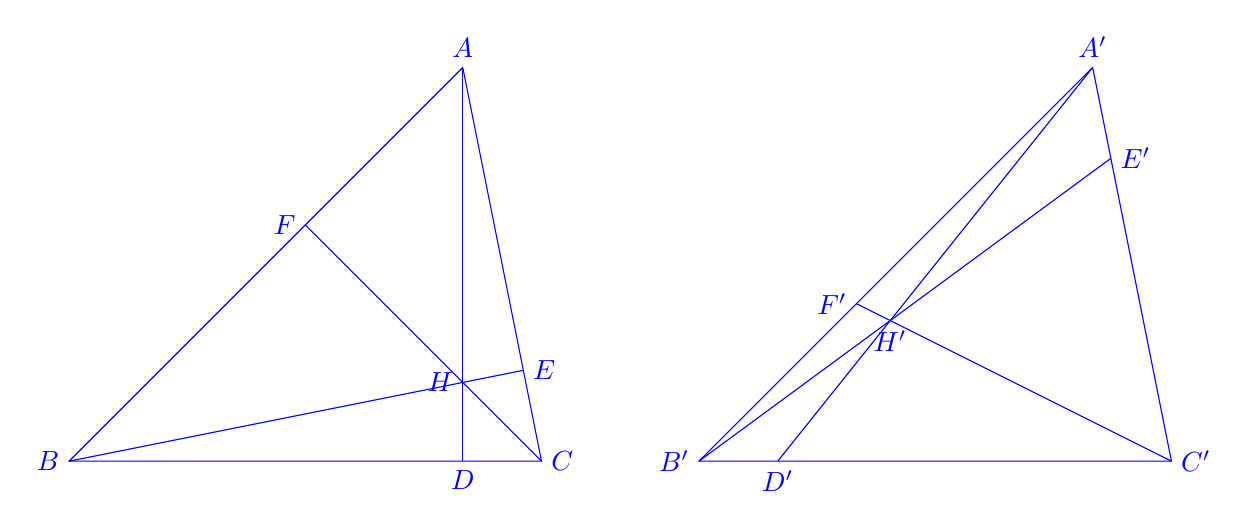
\begin{tikzpicture}
 \coordinate [label=above:\textcolor{blue}{$A$}] (A) at (5,5);
 \coordinate [label=left:\textcolor{blue}{$B$}] (B) at (0,0);
 \coordinate [label=right:\textcolor{blue}{$C$}] (C) at (6,0);
 \coordinate [label=below:\textcolor{blue}{$D$}] (D) at (5,0);
 \coordinate [label=left:\textcolor{blue}{$F$}](F) at (3,3);
 \coordinate [label=right:\textcolor{blue}{$E$}](E) at (150/26, 30/26);
 \coordinate [label=left:\textcolor{blue}{$H$}](H) at (5,1);
 
 \draw[blue] (A) -- (B) -- (C) -- (A);
 \draw[blue] (B) -- (E);
 \draw[blue] (C) -- (F);
 \draw[blue] (A) -- (D);
 
 \coordinate [label=above:\textcolor{blue}{$A'$}] (A') at (13,5);
 \coordinate [label=left:\textcolor{blue}{$B'$}] (B') at (8,0);
 \coordinate [label=right:\textcolor{blue}{$C'$}] (C') at (14,0);
 \coordinate [label=below:\textcolor{blue}{$D'$}] (D') at (9,0);
 \coordinate [label=left:\textcolor{blue}{$F'$}] (F') at (10,2);
 \coordinate [label=right:\textcolor{blue}{$E'$}] (E') at (172/13, 50/13);
 \coordinate [label=below:\textcolor{blue}{$H'$}] (H') at (73/7, 25/14);
 
  \draw[blue] (A') -- (B') -- (C') -- (A');
 \draw[blue] (B') -- (E');
 \draw[blue] (C') -- (F');
 \draw[blue] (A') -- (D');
\end{tikzpicture}
\ed

\bt{球面三角形余弦定理}{}
对于任给半径为$R$的球面三角形$\triangle ABC$, 其三边$a,b,c$和三角$\angle A, \angle B, \angle C$之间恒满足:
\begin{align*}
 \cos\frac{a}{R^2} & =\cos\frac{c}{R^2}\cos\frac{b}{R^2}+\sin\frac{b}{R^2}\sin\frac{c}{R^2}\cos\angle A,\\
 \cos\frac{b}{R^2} & =\cos\frac{a}{R^2}\cos\frac{c}{R^2}+\sin\frac{c}{R^2}\sin\frac{a}{R^2}\cos\angle B,\\
 \cos\frac{c}{R^2} & =\cos\frac{b}{R^2}\cos\frac{a}{R^2}+\sin\frac{a}{R^2}\sin\frac{b}{R^2}\cos\angle C.
\end{align*}
\et

\bt{球面三角形正弦定理}{}
条件同上, 有$\frac{\sin\angle A}{\sin\frac{a}{R^2}}=\frac{\sin\angle B}{\sin\frac{b}{R^2}}=\frac{\sin\angle C}{\sin\frac{c}{R^2}}$.
\et

\newpage

\section{不等式集}
\bq{}{}
已知$0\le a_k\le 1$($k=1,2,\cdots, 2002$), 记$a_{2003}=a_1$, $a_{2004}=a_2$, 求$\sum_{k=1}^{2002}(a_k-a_{k+1}\cdot a_{k+2})$的最大值.
\eq
\ba
\bee
\sum_{k=1}^{2002}(a_k-a_{k+1}\cdot a_{k+2})=\sum_{k=1}^{2002}(a_k-a_{k}a_{k+1})=\sum_{k=1}^{2002}a_{k}(1-a_{k+1}).
\eee
Cauchy不等式, 上式右端不超过
\bee
\sqrt{\left(\sum_{k=1}^{2002}a_k^2\right)\left(\sum_{k=1}^{2002}(1-a_{k+1})^2\right)}
\le \frac{\sum a_k^2 + \sum (1-a_{k+1})^2}{2}
=\frac{\sum a_k^2+\sum(1-a_k)^2}{2}
=\frac{\sum(2a_k^2-2a_k+1)}{2}.
\eee
因为$2a_k^2-2a_k+1\le1$, 所以原式不超过$\frac12\sum1=1001$, 当$a_k=0$或$1$时取等号, 即当$a_1=a_3=a_5=\cdots=a_{2001}=1$且$a_2=a_4=\cdots=a_{2002}=0$时取等号.
\ea
\ba
由$0\le a_k\le 1$, 得$(1-a_k)(1-a_{k+1})=1-(a_{k}+a_{k+1})+a_{k}a_{k+1}\ge0$($k=1,2,\cdots, 2002$), 所以$1\ge a_{k}+a_{k+1}-a_{k}a_{k+1}\ge a_{k}+a_{k+1}-2a_{k}a_{k+1}$,
从而$2002\ge\sum_{k=1}^{2002}(a_k+a_{k+1}-2a_{k}a_{k+1})=2\sum(a_k-a_{k+1}a_{k+2})$, 即$\sum(a_k-a_{k+1}a_{k+2})\le1001$.
\ea

\bq{}{}
求函数$y=x+\sqrt{x(2-x)}$的最值及此时$x$的值.
\eq
\ba
显然$x\in[0,2]$, 所以可设$x=2\sin^2\theta$($\theta\in\mathbb{R}$), 运用$|a\sin\theta+b\cos\theta|\le\sqrt{a^2+b^2}$即可.
\ea

\bq{}{}
设$n$是给定的正整数, $n\ge13$, 对$n$个给定的实数$a_1, a_2, \cdots, a_n$, 记$|a_i-a_j|$($1\le i < j\le n$)有最小值$m$, 求在$\sum_{i=1}^{n}a_i^2=1$的条件下, 
$m$的最大值.
\eq
\ba
不妨设$a_1\le a_2\le \cdots\le a_n$, 于是$a_2-a_1\ge m, a_3-a_2\ge m, \cdots, a_n-a_{n-1}\ge m$, $a_j-a_i\ge(j-i)m$($1\le i< j \le n$).
\bee
\sum_{1\le i<j\le n}(a_i-a_j)^2\ge m^2\times\sum_{1\le i<j\le n}(j-i)^2
=m^2\sum_{k=1}^{n-1}k(2k+1)(k+1)=\frac{m^2}{12}\cdot n^2(n^2-1).
\eee
另一方面, $\sum_{i=1}^{n}a_i^2=1$可得
\bee
\sum_{1\le i<j\le n}(a_i-a_j)^2=n-\left(\sum_{i=1}^{n}a_i\right)^2\le n.
\eee
故$n\ge\frac{m^2}{12}n^2(n^2-1)$, 所以$m\le\sqrt{\frac{12}{n^2(n^2-1)}}$, 当且仅当$\sum_{i=1}^{n}a_i=0$,
且$a_1, a_2, \cdots, a_n$成等差数列时取等号.
\ea

\bq{}{}
若$x,y,z>0$且$x^2+y^2+z^2=1$, 则$S=\frac{(z+1)^2}{2xyz}$取最小值时, $x$的值是多少?
\eq
\ba
$\sqrt{\sqrt{2}-1}$.
\ea

\bl{}{}
设$T\ge0$, $x, y, z\ge0$, 则$T\ge\sum x$的充要条件为:
\begin{align}
 & (T^2-\sum x^2)^2-8\prod x\cdot T-4\sum y^2z^2\ge0\label{20170327001}\\
 & T^2\ge\sum x^2.\label{20170327002}
\end{align}
\el
\ba
若$T\ge\sum x$, 则\ref{20170327002}式明显成立, 且
\bee
(T+\sum x)(T^2-\sum x^2+2\sum yz)-8\prod x
\ge2\sum x\cdot 4\sum yz-8\prod x
\ge0.
\eee
根据
\be
(T^2-\sum x^2)^2-8\prod x\cdot T-4\sum y^2z^2
=(T-\sum x)\left[(T+\sum x)(T^2-\sum x^2+2\sum yz)-8\prod x\right]\label{20170327003}
\ee
知\ref{20170327001}式成立. 若\ref{20170327001}, \ref{20170327002}式成立, 则
\bee
(T+\sum x)(T^2-\sum x^2+2\sum yz)-8\prod x
\ge (\sqrt{\sum x^2}+\sum x)\cdot 2\sum yz-8\prod x
\ge (\sqrt{3}+3)(\prod x)^{\frac13}\cdot6(\prod x)^{\frac23}-8\prod x\ge0.
\eee
根据\ref{20170327003}式知$T\ge\sum x$.
\ea
由引理即得
\bt{}{20170328001}
设$T\ge0$, $x,y,z\ge0$, 记$f=(T^2-\sum x^2)^2-8\prod x\cdot T-4\sum y^2z^2$, 则
\begin{enumerate}[(i)]
 \item 若$f\ge0$, $\sum x^2\le T^2$, 则$\sum x\le T$;
 \item 若$f\le 0$, 则$\sum x\ge T$.
\end{enumerate}
\et

\bq{}{}
\bee
\sum\cos\frac{A}{2}\le2+\frac{s}{4R}+\frac{9\sqrt{3}-16}{4R}r.
\eee
\eq
\ba
设$m=\frac{s}{4R}$, $n=\frac{r}{2R}$. 则$\sum\cos^2\frac{A}{2}=2+n$, $\prod\cos\frac{A}{2}=\frac{m}{2}$. 进而
\bee
\sum\cos^2\frac{A}{2}\cos^2\frac{B}{2}=\frac14(4+4n+m^2+n^2).
\eee
令$T=2+\frac{m}{2}+\frac{9\sqrt{3}-16}{2}n$, $x=\cos\frac{A}{2}$, $y=\cos\frac{B}{2}$, $z=\cos\frac{C}{2}$,
用定理\ref{th:20170328001}中结论(i).
\ea

\bq{}{}
设实数$a,b,c,d$, 满足$a^2+b^2+c^2+d^2=5$, 求$(a-b)^2+(a-c)^2+(a-d)^2+(b-c)^2+(b-d)^2+(c-d)^2$的最大值.
\eq
\ba
设$f=(a-b)^2+(a-c)^2+(a-d)^2+(b-c)^2+(b-d)^2+(c-d)^2=15-2(ab+ac+ad+bc+bd+cd)+\lambda(a^2+b^2+c^2+d^2-5)$,
所以$f_a=-2(b+c+d)+2a\lambda$, $f_b=-2(a+c+d)+2b\lambda$, $f_c=-2(a+b+d)+2c\lambda$, $f_d=-2(a+c+d)+2b\lambda$,
$f_{\lambda}=a^2+b^2+c^2+d^2-5$, 令$f_a=f_b=f_c=f_d=f_{\lambda}=0$, 解得$\lambda=-1$或$a=b=c=d$.
当$\lambda=-1$时, $a+b+c+d=0$得$f=20$.
当$a=b=c=d$时, $f=0$, 所以$f_{\max}=20$.
\ea

\bq{}{}
如果$x>0$, $y>0$, $z>0$且$x^2+y^2+z^2=1$, 求$\frac{yz}{x}+\frac{xz}{y}+\frac{xy}{z}$的最小值.
\eq
\ba
设$\frac{yz}{x}=a$, $\frac{xz}{y}-b$, $\frac{xy}{z}=c$, 则
$ab+bc+ca=1$, 所以$a^2+b^2+c^2\ge ab+bc+ca=1$, 所以$(a+b+c)^2=a^2+b^2+c^2+2(ab+bc+ca)\ge3$,
另外令$f=a+b+c+\lambda(ab+bc+ca-1)$, 令
$f_a=1+(b+c)\lambda=0$, $f_b=1+(a+c)\lambda=0$, $f_c=1+(a+b)\lambda=0$, 所以
$a=b=c$时最小.
\ea

\bq{}{}
设$a_0, a_1, a_2, \cdots, a_n$满足$a_0=\frac12$, $a_{k+1}=a_k+\frac{1}{n}a_k^2$, $k=0,1,2,\cdots, n-1$,
其中$n$是一个给定的正整数, 试证: $1-\frac{1}{n}<a_n<1$.
\eq
\ba
$a_n>a_{n-1}>a_{n-2}>\cdots>a_2>a_1>a_0=\frac{1}{2}$,
\begin{align*}
 \frac{1}{a_k}-\frac{1}{a_{k+1}}=\frac{1}{n+a_k}<\frac{1}{n} \Longrightarrow\frac{1}{a_0}-\frac{1}{a_n}<1,\\
 \frac{1}{a_k}-\frac{1}{a_{k+1}}=\frac{1}{n+a_k}>\frac{1}{n+1} \Longrightarrow\frac{1}{a_0}-\frac{1}{a_n}>\frac{n}{n+1}.
\end{align*}
\ea

\bq{}{}
当$a>1$时, 若不等式$\frac{1}{n+1}+\frac{1}{n+2}+\cdots+\frac{1}{2n}>\frac{7}{12}\left[\log_{a+1}x-\log_{a}x+1\right]$对于不小于2的正整数$n$恒成立,
求$x$的取值范围.
\eq
\ba
$a_{n}=\frac{1}{n+1}+\frac{1}{n+2}+\cdots+\frac{1}{2n}$递增, $x$的取值范围为$(1, +\infty)$.
\ea

\bq{}{}
实数集$\{a_0, a_1, a_2, \cdots, a_n\}$, 满足以下条件: 
\begin{enumerate}[(1)]
 \item $a_1=a_n=0$.
 \item 对$1\le k\le n-1$, 有$a_k=c+\sum_{i=k}^{n-1}a_{i-k}(a_i+a_{i+1})$.
\end{enumerate}
证明: $c\le\frac{1}{4n}$.
\eq
\ba
定义$S_k=\sum_{i=0}^ka_i$($k=0,1,2,\cdots, n$), 则
\begin{align*}
 S_n
 & =\sum_{k=0}^{n}a_k
 =\sum_{k=0}^{n-1}a_{k-1}
 =nc+\sum_{k=0}^{n-1}\sum_{i=k}^{n-1}a_{i-k}(a_i+a_{i+1})\\
 & =nc+\sum_{i=0}^{n-1}(a_i+a_{i+1})\cdot\sum_{k=0}^{i}a_{i-k}\\
 & =nc+\sum_{i=0}^{n-1}(a_i+a_{i+1})\sum_{t=0}^{i}a_t, (t=i-k)\\
 & =nc+\sum_{i=0}^{n-1}(a_i+a_{i+1})\cdot S_i\\
 & =nc+\left[S_1S_0+(S_2-S_0)S_1+(S_3-S_1)S_2+\cdots+(S_n-S_{n-2})S_{n-1}\right]
\end{align*}
即$S_n^2-S_n+nc=0$, $\Delta\ge0\Longrightarrow c\le\frac{1}{4n}$.
\ea

\bq{}{}
若关于$x$的不等式$\log_{\frac{1}{a}}(\sqrt{x^2+ax+5}+1)\cdot\log_{5}(x^2+ax+6)+\frac{1}{\log_{3}a}\ge0$,
求$a$的取值范围.
\eq
\ba
令$u=x^2+ax+5$, $\frac{\log_3(\sqrt{u}+1)}{-\log_3a}\cdot\log_5(u+1)+\frac{1}{\log_3a}\ge0$.
因为$f(4)=1$, 所以$a=2$.
\ea

\bq{}{}
设$a_1, a_2, \cdots, a_{2002}>0$且$\sum\frac{1}{2+a_i}=\frac12$, 求$\prod a_i$的最小值.
\eq
\ba
令$x_i=\frac{2}{2+a_i}$, 则$\sum x_i=1$, 则$a_i=2\cdot\frac{1-x_i}{x_i}$, 
因为
\begin{align*}
 \prod a_i
 & =2^{2002}\prod\frac{1-x_i}{x_i}\\
 & =2^{2002}\cdot\frac{1}{x_1x_2\cdots x_{2002}}\prod(x_1+x_2+\cdots+x_{i-1}+x_{i+1}+\cdots+x_{2002})\\
 & \ge2^{2002}\cdot\frac{1}{x_ix_2\cdots x_{2002}}\cdot2001^{2002}\cdot\prod\sqrt[2001]{x_1x_2\cdots x_{i-1}x_{i+1}\cdots x_{2002}}\\
 &=4002^{2002}.
\end{align*}
\ea

\bq{}{}
求最小的正数$\lambda$, 使得对任意正整数$n$, $a_i$和$b_i$, $b_i\in[1,2]$($i=1,2,\cdots, n$), 且$\sum_{i=1}^{n}a_{i}^2=\sum b_i^2$, 
都有$\sum\frac{a_i^3}{b_i}\le\lambda\cdot\sum a_i^2$.
\eq
\ba
对任意$c_i, b_i\in[1,2]$, 有$\frac{1}{2}\le\frac{c_i}{b_i}\le 2$, 即$\frac{1}{2}b_i\le c_i\le2b_i$,
从而$\left(\frac{1}{2}b_i-c_i\right)(2b_i-c_i)\le0$, 即$c_i^2+b_i^2\le\frac{5}{2}c_ib_i$,
两边对$i$从1到$n$求和, 得$\sum c_i^2+\sum b_i^2\le\frac{5}{2}\sum c_ib_i$,
设$a_i, b_i\in\left[1, \frac{2}{3}\right]$, 因$a_i^2=\frac{a_i^{\frac{3}{2}}}{b_i^{\frac{1}{2}}}\cdot a_i^{\frac{1}{2}}\cdot b_i^{\frac{1}{2}}$.
又
\bee
\frac{1}{2}\le\frac{\frac{a_i^{\frac{3}{2}}}{b_{i}^{\frac{1}{2}}}}{a_i^{\frac{1}{2}}\cdot b_i^{\frac{1}{2}}}\le 2.
\eee
故有$\frac{5}{2}\sum a_i^2\ge\sum\frac{a_i^3}{b_i}+\sum a_ib_i\ge\sum\frac{a_i^3}{b_i}+\frac{2}{5}(\sum a_i^2+\sum b_i^2)=\sum\frac{a_i^3}{b_i}+\frac{4}{5}\sum a_i^2$,
即$\sum\frac{a_i^3}{b_i}\le\frac{17}{10}\sum a_i^2$, 当$n=2$, $a_1=1$, $a_2=2$, $b_1=2$, $b_2=1$时取等号.
\ea

\bq{}{}
已知: $x,y,z\in\mathbb{R}^*$, 有$xyz=1$且满足$x(1+z)>1$, $y(1+x)>1$, $z(1+y)>1$, 
求证: $2(x+y+z)\ge\frac{1}{x}+\frac{1}{y}+\frac{1}{z}+3$.
\eq
\ba
令$x=\frac{a}{b}$, $y=\frac{b}{c}$, $z=\frac{c}{a}$, 则$a+c>b$, $a+b>c$, $b+c>a$, 要证$2(x+y+z)\ge\frac1x+\frac1y+\frac1z+3$, 只需证
\bee
2\left(\frac{a}{b}+\frac{b}{c}+\frac{c}{a}\right)\ge\frac{b}{a}+\frac{c}{b}+\frac{a}{c}+3\Longleftrightarrow
  2(a^2c+b^2a+c^2b)\ge b^2c+c^2a+a^2b+3abc.
\eee
因为
\bee
(a+b-c)(b-c)^2\ge0, \quad (b+c-a)(c-a)^2\ge0, \quad (c+a-b)(a-b)^2\ge0
\eee
展开相加, 即得.
\ea

\bq{}{}
已知正整数$n\ge 2$, 若对同时满足条件:
\begin{enumerate}[(1)]
 \item $a_1a_2\cdots a_n=b_1 b_2\cdots b_n$;
 \item $\sum_{1\le i<j\le n}|a_i-a_j|\le \sum_{1\le i<j\le n}|b_i-b_j|$的任意正数$a_1,\cdots, a_n$与$b_1,\cdots, b_n$,
 总有$\sum_{i=1}^{n}a_i\le\lambda\sum_{i=1}^{n}b_i$. 试求正数$\lambda$的最小值.
\end{enumerate}
\eq
\ba
一方面, 取$(a_1,\cdots, a_n)=(1,1,\cdots,(1+x)x^{n-1})$, $(b_1,\cdots,b_n)=(1+x,x,x,\cdots, x)$, 满足(1)与(2), 
此时$\lambda\ge\frac{\sum a_i}{\sum b_i}=\frac{n-1+x^{n-1}+x^n}{1+nx}$, 令$x\to0$, 则$\lambda\ge n-1$.

以下证明$\lambda=n-1$时, 不等式成立.

不妨设$a_1\ge a_2\ge\cdots\ge a_n$, $b_1\ge b_2\ge \cdots\ge b_n$, $n=2$时, 显然成立.

设$n\ge3$,

(1) 若$a_1\le\frac{n-1}{n}b_1$, 则$\sum a_i\le na_1\le(n-1)b_1\le(n-1)\sum b_i$.

(2) 若$a_1>\frac{n-1}{n}b_1$, 则
\begin{align*}
 2(b_2+\cdots+b_n) & \ge 2(n-1)\cdot(b_2\cdots b_n)^{\frac{1}{n-1}}=2(n-1)\left(\frac{a_1}{b_1}a_2\cdots a_n\right)^{\frac{1}{n-1}}\\
  & \ge 2(n-1)\left(\frac{a_1}{b_1}\right)^{\frac{1}{n-1}}\cdot a_n>2(n-1)\cdot\left(\frac{n-1}{n}\right)^{\frac{1}{n-1}}\cdot a_n\\
  & \ge na_n.
\end{align*}
所以
\begin{align*}
 (n-1)\sum b_i &= (n-1)b_1+(n-3)\sum_{i=2}^{n}b_i+2\sum_{i=2}^{n}b_i\\
  &\ge(n-1)b_1+(n-3)\sum_{i=2}^{n}b_i+na_n\ge[(n-1)b_1+(n-3)b_2+\cdots-(n-1)b_n]+na_n\\
  &=\sum_{1\le i<j\le n}|b_i-b_j|+na_n\ge\sum_{1\le i<j\le n}|a_i-a_j|+na_n\\
  &=[(n-1)a_1+(n-3)a_2+\cdots-(n-1)a_n]+na_n\\
  &\ge(n-1)a_1+a_n\ge a_1+a_2+\cdots+a_{n-1}+a_n.
\end{align*}
\ea

\bq{1998年上海市高中数学竞赛}{}
设非零多项式$f(x)=a_nx^n+a_{n-1}x^{n-1}+\cdots+a_0$, $g(x)=c_{n+1}x^{n+1}+c_nx^n+\cdots+c_0$, 满足$g(x)=(x+r)f(x)$, 其中$r$为一实数,
设$a=\max(|a_{n}|, |a_{n-1}|,\cdots,|a_0|)$, $c=\max(|c_{n+1}|,|c_{n}|,\cdots,|c_0|)$, 求证: $\frac{a}{c}\le n+1$.
\eq
\ba
设$|r|\le1$, 由$\sum_{i=0}^{n+1}c_ix^i=(x+r)\sum_{i=0}^{n}a_ix^i=a_nx^{n+1}+\sum_{i=1}^{n}(ra_i+a_{i-1})x^i+ra_0$. 
故
\bee
\begin{dcases}
 c_{n+1}=a_n\\
 c_{n}=ra_n+a_{n-1}\\
 \cdots\\
 c_{1}=ra_1+a_0\\
 c_0=ra_0
\end{dcases}
\Longrightarrow
\begin{dcases}
 a_{n}=c_{n+1}\\
 a_{n-1}=-rc_{n+1}+c_n\\
 a_{n-2}=(-r)^2c_{n+1}+(-r)c_n+c_{n-1}\\
 \cdots\\
 a_0=(-r)^nc_{n+1}+(-r)^{n-1}c_n+\cdots+c_1,
\end{dcases}
\eee
故$|a|=|a_i|=|(-r)^{n-i}c_{n+1}+\cdots+c_{i+1}|\le|c_{n+1}|+\cdots+|c_{i+1}|\le(n-i+1)c\le(n+1)c$.

如果$|r|>1$, 令$x=\frac{1}{x}$, 代入$g(x)=(x+r)f(x)$, 则转化为上述情形, 仍有$a\le(n+1)c$.

另外
\bee
  |a|=|a_i|\le|r|^{n-i}|c_{n+1}|+\cdots+|c_{i+1}|\le(|r^n|+|r^{n-1}|+\cdots+1)c\le\frac{|r|^{n+1}-1}{|r|-1}c
\eee
而
\bee
\frac{|r|^{n+1}-1}{|r|-1}\le n+1
\Longleftrightarrow |r|^{n+1}\ge n|r|-n+|r|
\Longleftrightarrow |r|^n+\frac{n}{|r|}\ge n+1
\Longleftrightarrow |r|^n+\frac{1}{|r|}+\cdots+\frac{1}{|r|}\ge n+1
\eee

($|r|=0$时, 命题显然成立).
\ea

\bq{}{}
若$a,b,c\in\mathbb{R}$, 且$5a^4+4b^4+6c^4=90$, 求$5a^3+2b^3+3c^3$的最大值.
\eq
\ba
只需考虑$a,b,c\in\mathbb{R}^*$. 因$a^3=\frac12(a\cdot a\cdot a\cdot2)\le\frac{1}{8}(a^4+a^4+a^4+2^4)=\frac38a^4+2$,
同理$b^3\le\frac34b^4+\frac14$, $c^3\le\frac34c^4+\frac14$, 所以所求最大值为$45$.
\ea

\bq{}{}
若$x,y,z$为实数, $0<x<y<z<\frac{\pi}{2}$, 证明: $\frac{\pi}{2}+2\sin x\cos y+2\sin y\cos z>\sin 2x+\sin 2y+\sin 2z$.
\eq
\ba
原不等式等价于证明$\frac{\pi}{4}>\sin x(\cos x-\cos y)+\sin y(\cos y-\cos z)+\sin z\cos z$. 如图所示
\begin{center}
 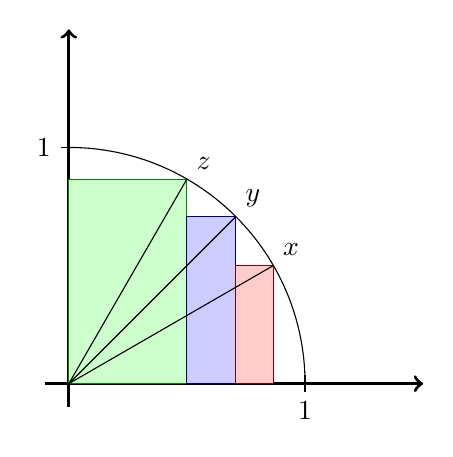
\begin{tikzpicture}[scale=3]
  \draw[->,very thick] (-.1,0) -- (1.5,0) coordinate (x axis);
  \draw[->,very thick] (0,-0.1) -- (0,1.5) coordinate (y axis);
  \draw (1,0) arc [start angle=0,end angle=90,x radius=1cm,y radius=1cm];
  let x=30;
  let y=45;
  let z=60;
  \filldraw[fill=green!20, draw=green!50!black] (0,0) -- (0.5,0) -- (0.5,0.866) -- (0,0.866) -- cycle;
  \filldraw[fill=blue!20, draw=blue!50!black] (0.5,0) -- (0.707,0) -- (0.707,0.707) -- (0.5,0.707) -- cycle;
  \filldraw[fill=red!20, draw=red!50!black] (0.707,0) -- (0.866,0) -- (0.866,0.5) -- (0.707,0.5) -- cycle;
  \draw (0,0) -- (0.866,0.5) node [anchor=south west] {$x$};
  \draw (0,0) -- (0.707,0.707) node [anchor=south west] {$y$};
  \draw (0,0) -- (0.5,0.866) node [anchor=south west] {$z$};
  \draw (1,1pt) -- (1,-1pt) node [anchor=north] {$1$};
  \draw (1pt,1) -- (-1pt,1) node [anchor=east] {$1$};
  \end{tikzpicture}
\end{center}
\ea

\bq{1987年第21届全苏MO}{}
正数$a,b,c,A,B,C$满足条件$a+A=b+B=c+C=k$, 求证: $aB+bC+cA<k^2$.
\eq
\ba
主试委员会给出的解答是$k^3=(a+A)(b+B)(c+C)$, 利用放缩的技巧给出证明, 北京四中的袁峰同学给出了如下构造性证明.

如图: $S_{\triangle LRM}+S_{\triangle PNM}+S_{\triangle QLN}<S_{\triangle PQR}$, 化简即得.
\begin{center}
 \begin{tikzpicture}[scale=3]
  \coordinate [label=left:$Q$] (Q) at (0,0);
  \coordinate [label=above:$P$] (P) at (0.5,0.866);
  \coordinate [label=right:$R$] (R) at (1,0);
  \draw (P) -- (Q) -- (R) -- cycle;
  \coordinate [label=below:$L$] (L) at ($ (R) !0.7! (Q) $);
  \coordinate [label=right:$M$] (M) at ($ (P) !0.4! (R)$);
  \coordinate [label=left:$N$] (N) at ($ (P) !0.5! (Q)$);
  \draw (L) -- (M) -- (N) -- cycle;
  \node (A) [label=below:$A$] at ($ (Q) !0.5! (L) $) {};
  \node (a) [label=below:$a$] at ($ (R) !0.5! (L) $) {};
  \node (B) [label=right:$B$] at ($ (M) !0.5! (R) $) {};
  \node (b) [label=right:$b$] at ($ (P) !0.5! (M) $) {};
  \node (C) [label=left:$C$] at ($ (P) !0.5! (N) $) {};
  \node (c) [label=left:$c$] at ($ (N) !0.5! (Q) $) {};
  
  \foreach \point in {P,Q,R,L,M,N}
    \fill [blue,opacity=.75] (\point) circle (1pt);
 \end{tikzpicture}

\end{center}

\ea
\ba
如图:
\begin{center}
 \begin{tikzpicture}[scale=3]
  \coordinate[label=225:$P$] (P) at (0,0);
  \coordinate[label=315:$Q$] (Q) at (1,0);
  \coordinate[label=45:$R$] (R) at (1,1);
  \coordinate[label=135:$S$] (S) at (0,1);
  
  \draw (P) -- (Q) -- (R) -- (S) -- cycle;
  \filldraw[fill=yellow!80!black,opacity=0.5] (P) rectangle (0.6,0.4);
  \filldraw[fill=red!80!black,opacity=0.5] (0.6,0) rectangle (1,0.7);
  \filldraw[fill=blue!80!black,opacity=0.5] (1,0.7) rectangle (0.3,1);
  
  \node [label=below:$B$] at ( $ (P) !0.5! (0.6,0) $) {};
  \node [label=below:$b$] at ( $ (Q) !0.5! (0.6,0) $) {};
  \node [label=right:$C$] at ( $ (Q) !0.5! (1,0.7) $) {};
  \node [label=right:$c$] at ( $ (R) !0.5! (1,0.7) $) {};
  \node [label=above:$A$] at ( $ (R) !0.5! (0.3,1) $) {};
  \node [label=left:$a$] at ( $ (P) !0.5! (0,0.4) $) {};
  
  \foreach \point in {P,Q,R,S}
    \fill [blue,opacity=.75] (\point) circle (1pt);
 \end{tikzpicture}

\end{center}

\ea

\bq{第31届IMO预选题}{}
设集合$\{a_1,a_2,\cdots,a_n\}=\{1,2,\cdots,n\}$, 求证:
\bee
\frac12+\frac23+\cdots+\frac{n-1}{n}\le\frac{a_1}{a_2}+\frac{a_2}{a_3}+\cdots+\frac{a_{n-1}}{a_n}.
\eee
\eq
\ba
设$b_1,b_2,\cdots,b_{n-1}$是$a_1,a_2,\cdots,a_{n-1}$的一个排列, 且$b_1<b_2<\cdots<b_{n-1}$, 
$c_1,c_2,\cdots,c_{n-1}$是$a_2,a_3,\cdots,a_{n}$的一个排列, 且$c_1<c_2<\cdots<c_{n-1}$, 则
\bee
\frac1{c_1}>\frac1{c_2}>\cdots>\frac1{c_{n-1}}.
\eee
且$b_1\ge1$, $b_2\ge2$, $\cdots,b_{n-1}\ge n-1$, $c_1\le 2,c_2\le3,\cdots,c_{n-1}\le n$,
由排序不等式得:
\bee
\frac{a_1}{a_2}+\frac{a_2}{a_3}+\cdots+\frac{a_{n-1}}{a_n}
  \ge \frac{b_1}{c_1}+\frac{b_2}{c_2}+\cdots+\frac{b_{n-1}}{c_{n-1}}
  \ge \frac12+\frac23+\cdots+\frac{n-1}{n}.
\eee
这是南斯拉夫提给第31届IMO的一道试题, 原证法是利用加强命题的手法, 用数学归纳法给出证明.
一则加强命题很难想到, 二则归纳法证明要对足标进行讨论, 比较麻烦. 在当年国家集训队里姚建钢同学(第35届IMO金牌得主)的证法,
更是干脆, 漂亮, 出人意料.
\ea
\ba
易证
\bee
\prod_{k=1}^{n-1}(a_k+1)\ge\prod_{k=1}^na_k,
\eee
故
\begin{align*}
 \sum_{k=1}^{n-1}\frac{a_k}{a_{k+1}}+\paren{\sum_{k=1}^n\frac1k}
  &=\frac{1}{a_1}+\sum_{k=1}^{n-1}\frac{a_k+1}{a_{k+1}}\\
  &\ge n \sqrt[n]{\frac{\prod_{k=1}^{n-1}(a_k+1)}{\prod_{k=1}^na_k}}\ge n\\
  &=\sum_{k=1}^{n}\frac{1}{k}+\sum_{k=1}^{n-1}\frac{k}{k+1}
\end{align*}

\ea

\bq{第24届IMO}{}
设$a,b,c$分别为一个三角形的三边之长, 求证:
\bee
a^2b(a-b)+b^2c(b-c)+c^2a(c-a)\ge0.
\eee
并指出等号成立的条件.
\eq
\ba
原联邦德国选手伯恩哈德$\cdot$里普只用了一个等式:
\bee
a^2b(a-b)+b^2c(b-c)+c^2a(c-a)
  = a(b-c)^2(b+c-a)+b(a-b)(a-c)(a+b-c)
\eee
由轮换对称性, 不妨设$a\ge b, c$, 即得欲证不等式成立, 而且显然等号成立的充要条件是$a=b=c$.

里普的证法新颖, 巧妙, 简洁, 与主试委员会提供的参考答案不同, 他因此获得了该届的特别奖.
\ea

\bq{1980年芬兰, 英国, 匈牙利, 瑞典四国联赛}{}
设数列$a_0,a_1,\cdots,a_n$满足$a_0=\frac12$及$a_{k+1}=a_k+\frac1na_k^2$($k=0,1,2,\cdots,n-1$),
其中$n$是一个给定的正整数, 试证:
\bee
1-\frac1n<a_n<1.
\eee
\eq
\ba
该题是该次竞赛得分率最低的一道试题, 主试委员会所给出的解法也相当繁琐, 前后共用了四次归纳法, 译成中文后有4000多字,
中国科技大学白志东先生对此题采用了大胆的处理方法, 加强命题, 出奇制胜给出一个简洁的证明.

由于$a_1=a_0+\frac1na_0^2=\frac12+\frac1{4n}=\frac{2n+1}{4n}$, 所以
\bee
\frac{n+1}{2n+1}<a_1<\frac{n}{2n-1}.
\eee
我们来用归纳法证: 对于一切$1\le k\le n$, 都有
\be\label{20180704001}
\frac{n+1}{2n-k+2}<a_k<\frac{n}{2n-k}.
\ee
假设(\ref{20180704001})对于$k<n$成立, 则
\bee
a_{k+1}=a_k\paren{1+\frac1na_k}
  <\frac{n}{2n-k}\paren{1+\frac1{2n-k}}
  =\frac{n(2n-k+1)}{(2n-k)^2}
  <\frac{n}{2n-(k+1)}.
\eee
所以
\begin{align*}
 a_{k+1} & = a_k+\frac1na_k^2>\frac{n+1}{2n-k+2}+\frac{(n+1)^2}{n(2n-k+2)^2}\\
  &>\frac{n+1}{2n-(k+1)+2}
\end{align*}
于是(\ref{20180704001})式对于一切$1\le k\le n$均成立, 特别在$k=n$时,
\bee
1-\frac1n<\frac{n+1}{n+2}<a_n<\frac{n}{n}=1.
\eee

{\bf{说明}} 这里所证的不等式(\ref{20180704001})式比题目所要证明的不等式强, 却收到了事半功倍之效,
下面给出一种直接了当的证明.
\ea
\ba
由已知, 
\bee
\frac1{a_{k-1}}-\frac1{a_k}=\frac1{n+a_{k-1}},
\eee
从而$a_n>a_{n-1}>\cdots>a_1>a_0=\frac12$. 所以
\bee
\frac1{a_{k-1}}-\frac1{a_k}<\frac1n,\quad k=1,2,\cdots,n.
\eee
累加得$\frac1{a_0}-\frac1{a_n}>\frac{n}{n+1}$, 所以$\frac{1}{a_n}<2-\frac{n}{n+1}=\frac{n+2}{n+1}$.
\ea

\bq{}{}
已知函数$f(x)$的定义域为$\RR$, 对于任意实数$m,n$均有$f(m+n)=f(m)+f(n)-1$, 且$f\paren{\frac12}=2$, 
当$x>-\frac12$时, 恒有$f(x)>0$, 求证: $f(x)$单调递增.
\eq
\ba
证明: 令$x_1>x_2$, 所以
\bee
f(x_1)-f(x_2)=f(x_1-x_2)-1
  =f\paren{\paren{x_1-x_2-\frac12}+\frac12}-1
  =f\paren{x_1-x_2-\frac12}+f\paren{\frac12}-1-1
  =f\paren{x_1-x_2-\frac12}
\eee
因为$x_1-x_2-\frac12>-\frac12$, 所以$f\paren{x_1-x_2-\frac12}>0$, 
所以$f(x_1)>f(x_2)$, 得证.
\ea

\bq{}{}
已知: 正数$x,y,z$均小于$1$且$x+y+z=2$, $w=xy+yz+zx$, 求$w$的取值范围.
\eq
\ba
易得$w\le\frac43$, 令$x(1-x)=a^2$, $y(1-y)=b^2$, $z(1-z)=c^2$, 因为
\bee
w=xy+z(2-z)=xz+y(2-y)=yz+x(2-x)
\eee
所以
\bee
3w=w+2\times2-x^2-y^2-z^2=w+4+a^2+b^2+c^2-2
\eee
所以$2w=2+a^2+b^2+c^2\ge2$, 即$w\ge1$.
仅当$a,b,c=0$时取$w=1$, 但$a,b,c\ne0$, 所以$w>1$.
\ea

\bq{}{}
已知$\frac{a^2+b^2}{4}+c^2=1$, 求$a+b+c$的最大值.
\eq
\ba
\begin{align*}
 (a+b+c)^2 = & a^2+b^2+c^2+2bc+2ab+2ac\\
  \le & a^2+b^2+c^2+(a^2+b^2)+\paren{\frac{b^2}{4}+4c^2}+\paren{\frac{a^2}{4}+4c^2}\\
  = & 9\paren{\frac{a^2+b^2}{4}}=9.
\end{align*}
\ea

\bq{}{}
已知$a,b>0$, $a+b=1$, 证明: $\frac32<\frac1{a^2+1}+\frac1{b^2+1}\le\frac85$.
\eq
\ba
原式等价于证明:
\begin{align*}
 15(a^2+1)(b^2+1)<10(a^2+b^2+2)\le16(a^2+1)(b^2+1)
  & \Longleftrightarrow 15a^2b^2+5a^2+5b^2-5<0\le16a^2b^2+6a^2+6b^2-4\\
  & \Longleftrightarrow 3a^2b^2+a^2+b^2-1<0\le8a^2b^2+3a^2+3b^2-2.
\end{align*}
因$a+b=1$, 所以$a^2+b^2-1=-2ab$. 所以上式等价于
\bee
3a^2b^2-2ab<0\le8a^2b^2-6ab+1.
\eee
又由$a^2+b^2+2ab=1\ge4ab$, 所以$0<ab\le\frac14$, 所以上式成立.
\ea
\ba
令$a=\sin^2\theta, b=\cos^2\theta$, $\paren{0<\theta<\frac{\pi}{2}}$, 所以
\begin{align*}
\frac1{a^2+1}+\frac1{b^2+1}
  &=\frac1{1+\sin^4\theta}+\frac1{1+\cos^4\theta}\\
  &=\frac4{5-2\cos2\theta+\cos^22\theta}+\frac4{5+2\cos2\theta+\cos^22\theta}\\
  &=\frac{16(11+\cos4\theta)}{(11+\cos4\theta)^2-8(11+\cos4\theta)+80}\\
  &=\frac{16y}{y^2-8y+80}=\frac{16}{y+\frac{80}{y}-8}
\end{align*}
因$0<\theta<\frac{\pi}{2}$, 所以$0<4\theta<2\pi$. 所以$10<y\le12$, 并有$\frac32<\frac{16}{y+\frac{80}{y}-8}\le\frac85$.
\ea

\bq{}{}
已知数列$\{a_n\}$, $\{b_n\}$, $\{c_n\}$满足: $b_n=a_n-a_{n+2}$, $c_n=a_n+2a_{n+1}+3a_{n+2}$, ($n=1,2,3,\cdots$),
若$\{c_n\}$为等差数列且$b_n\le b_{n+1}$, 证明: $b_n=b_{n+1}$.
\eq
\ba
由于$a_n-a_{n+2}=b_{n}\le b_{n+1}\le b_{n+2}=a_{n+2}-a_{n+4}$, 所以$2a_{n+2}\ge a_n+a_{n+4}$.
因为$2c_{n+1}=c_n+c_{n+2}$, 所以$4a_{n+3}=a_{n}+3a_{n+4}\le 2a_{n+2}+2a_{n+4}$, 
所以$2a_{n+3}\le a_{n+2}+a_{n+4}$. 所以$a_{n+3}-a_{n+2}\le a_{n+4}-a_{n+3}\le a_{n+5}-a_{n+4}$, 
所以$a_{n+3}-a_{n+5}\le a_{n+2}-a_{n+4}$, 所以$b_{n+3}\le b_{n+2}\le b_{n+3}$,
所以$b_{n+3}=b_{n+2}$, ($n\ge1$). 所以$b_3=b_4=b_5=\cdots=-2d=a_3-a_5=a_4-a_6=a_5-a_7$, 
所以
\begin{align*}
 4a_5-3a_6=a_2\le a_3-a_5+a_4
 &\Longrightarrow 5a_5\le a_3+a_4+3a_6\\
 &\Longrightarrow 5(a_3+2d)\le a_3+a_4+3(a_4+2d)\\
 &\Longrightarrow 2a_3\le2a_4-2d=2a_4+a_3-a_5\\
 &\Longrightarrow a_3+a_5\le 2a_4.
\end{align*}
因$a_3+a_5\ge2a_4$, 所以$a_2=a_3-a_5+a_4$, 同理$a_1=a_2-a_4+a_3$,
即$b_1=b_2=b_3=\cdots$.

两个正数$a,b$的和一定时, 它们的积
\be
ab=\frac14\paren{(a+b)^2-(a-b)^2}
\ee
随着差$\abs{a-b}$的增大而减小;
其平方和
\be
a^2+b^2=\frac12\paren{(a+b)^2+(a-b)^2}
\ee
随着差$\abs{a-b}$的增大而增大.
\ea

\bq{}{}
已知$\triangle ABC$的三边, $a, b,c$成等比数列, 则$\sin B+\cos B$的取值范围为\underline{$\qquad$}.
\eq
\ba
命题等价于$a+b>c$, $a+c>b$, $b+c>a$, $b^2=ac$,
\bee
b^2=ac=a^2+c^2-2ac\cos B\ge2ac-2ac\cos B,
\eee
所以$\cos B\ge\frac12$, $0<B\le60^{\circ}$, 由$\frac12\le\cos B<1$及$0<\sin B\le\frac{\sqrt{3}}{2}$,
所以
\be\label{20180705001}
\frac12<\cos B+\sin B<\frac{\sqrt{3}}{2}+1,
\ee
另一方面, $\sin B+\cos B=\sqrt{2}\sin(B+45^{\circ})$, 而$45^{\circ}<B+45^{\circ}<105^{\circ}$,
故
\be\label{20180705002}
1<\sin B+\cos B\le \sqrt{2}.
\ee
综合(\ref{20180705001}), (\ref{20180705002})有$1<\sin B+\cos B\le\sqrt{2}$.
\ea

\bq{}{}
设$a,b,c$是直角$\triangle ABC$的三边长, $c$为斜边, 求使不等式
\bee
a^2(b+c)+b^2(c+a)+c^2(a+b)\ge kabc
\eee
恒成立的$k$的最大值.
\eq
\ba
$a>0, b>0, c>0$, $c^2=a^2+b^2$, 所以
\begin{align*}
 LHS&=(a^2+b^2)c+a\paren{b^2+\frac{c^2}{2}}+b\paren{\frac{c^2}{2}+a^2}+\frac{c}{2}\cdot c(a+b)\\
  &\ge 2abc+\sqrt{2}abc+\sqrt{2}abc+\frac{c}{2}\sqrt{a^2+b^2}\cdot2\sqrt{ab}\\
  &\ge (2+2\sqrt{2})abc+c\cdot\sqrt{2ab}\cdot\sqrt{ab}=(2+3\sqrt{2})abc,
\end{align*}
仅当$a=b$时上式取等号.
\bee
(a+b+c)\paren{\frac1a+\frac1b+\frac1c}\ge5+3\sqrt{2}.
\eee
\ea

\bq{}{}
设$x_1$是方程$\sqrt{3}\sin x-3\cos x=2a-1$的最大负根, $x_2$是方程$2\cos^2 x-2\sin^2x=a$的最小正根,
求使不等式$\abs{x_1}\le x_2$成立的实数$a$的取值范围.
\eq
\ba
方程$\sqrt{3}\sin x-3\cos x=2a-1$等价于$\sin\paren{x-\frac{\pi}{3}}=\frac{2a-1}{2\sqrt{3}}$, 
从而得到$-1\le \frac{2a-1}{2\sqrt{3}}\le 1$. 解得$\frac12-\sqrt{3}\le a\le \frac12+\sqrt{3}$, 而且
\bee
x_1=
\begin{cases}
	\frac{\pi}{3}+\arcsin\frac{2a-1}{2\sqrt{3}}, & \paren{\frac12-\sqrt{3}\le a<-1}\\
	-\frac{2\pi}{3}-\arcsin\frac{2a-1}{2\sqrt{3}}, & \paren{-1\le a\le\frac12+\sqrt{3}}
\end{cases}
\eee
其图像如图, 位于$a$轴下方, 方程$2\cos^2x-2\sin^2x=a$等价于$\cos 2x=\frac{a}{2}$,
其中$-1\le\frac{a}{2}\le 1$, 所以$-2\le a\le 2$, 解得
\bee
x_2=
\begin{cases}
	\frac12\arccos\frac{a}{2}, & (-2<a\le 2)\\
	\pi, & (a=2).
\end{cases}
\eee
其图像如图, 它位于$a$轴上方, 比较两个函数的图像, 不难看出$|x_1|\le x_2$的充要条件是$\frac12-\sqrt{3}\le a\le -1$或$a=2$.
\begin{center}
 \begin{tikzpicture}
  \begin{axis}[
    axis equal,
    axis lines=middle,
    axis line style={->},
    xlabel={$a$},
    ylabel={$x$},
    ]
   \addplot[blue,thick] gnuplot [domain=-1.232:-1,samples=120] {pi/3+asin((2*x-1)/(2*sqrt(3)))};
   \addplot[blue,thick] gnuplot [domain=-1:2.232,samples=120] {-2*pi/3-asin((2*x-1)/(2*sqrt(3)))};
   \addplot[blue,thick] gnuplot [domain=-2:2,unbounded coords=jump,samples=120] {0.5*acos(x/2)};
   \addplot[
    scatter,
    only marks,
    nodes near coords,
    point meta=explicit symbolic,
    scatter/classes={
      o={mark=*,fill=white},
      c={mark=*,blue}},
   ] table[meta=label] {
      x		y	label
      2	3.14	c
      2	0	o
      -2	1.57	c
      -1	0	o
      -1.232	-0.52	c
      -1	-1.04	c
      2.232	-3.66	c
    };
    \addplot [color=blue, thick, dashed] coordinates {(2,0) (2,3.14) (0,3.14)};
    \addplot [color=blue, thick, dashed] coordinates {(-2,0) (-2,1.57) (0,1.57)};
    \addplot [color=blue, thick, dashed] coordinates {(-1.232,0) (-1.232,-0.52) (0,-0.52)};
    \addplot [color=blue, thick, dashed] coordinates {(-1,0) (-1,-1.04) (0,-1.04)};
    \addplot [color=blue, thick, dashed] coordinates {(2.232,0) (2.232,-3.66) (0,-3.66)};
    \addplot+[only marks,nodes near coords,blue,point meta=explicit symbolic] coordinates {
      (-2,1.57) [$(-2,\frac{\pi}{2})$]
      (2,3.14) [$(2,\pi)$]
    };
  \end{axis}
 \end{tikzpicture}
\end{center}
\ea

\bq{}{}
函数$y=\sqrt{8x-x^2}-\sqrt{14x-x^2-48}$的最大值为\underline{$2\sqrt{3}$}, 最小值为\underline{0}.
\eq
\ba
$x$的定义域为$6\le x \le 8$, 而
\bee
f(x)=\frac{6\sqrt{8-x}}{\sqrt{x}+\sqrt{x-6}}
\eee
在$[6,8]$上递减.
\ea

\bq{}{}
已知$a,b,c,d\in\RR$, 满足$a+b+c+d=3$, $a^2+2b^2+3c^2+6d^2=5$, 
则$a$的最小值与最大值的和是\underline{3}.
\eq
\ba
\bee
5-a^2=2b^2+3c^2+6d^2=\frac16(3+2+1)(2b^2+3c^2+6d^2)\ge(b+c+d)^2=(3-a)^2.
\eee
\ea

\bq{}{}
用$\delta(S)$表示非零整数集$S$中所有元素的和, 设$A=\{a_1,a_2,\cdots,a_{11}\}$是正整数集,
且$a_1<a_2<\cdots<a_{11}$, 若对每个正整数$n\le1500$, 存在$A$的子集$S$, 使得$\delta(S)=n$,
求满足上述要求的$a_{10}$的最小值.
\eq
\ba
令$S_k=a_1+a_2+\cdots+a_k$, ($1\le k\le 11$), 若$a_k>S_{k-1}+1$,
则不存在$S\subset A$, 使$\delta(S)=S_{k-1}+1$, 所以$S_k=S_{k-1}+a_k\le2S_{k-1}+1$.
又由题设得$S_1=a_1=1$, 于是由归纳法易得$S_k\le2^k-1$, ($1\le k\le m$).
若$S_{10}<750$, 则$a_{11}\le750$, (否则$750$无法用$\delta(S)$表出),
$S_{11}=S_{10}+a_{11}<1500$, 所以$S_{10}\ge750$.
又$S_{8}\le2^8-1=255$, 所以$2a_{10}\ge a_{9}+a_{10}=S_{10}-S_8\ge495$,
$a_{10}\ge248$, 另一方面, 令$A=\{1,2,4,8,16,32,64,128,247,248,750\}$合题意.
\ea

\bq{}{}
$a,b,c>0$, $l^2=a^2+b^2+c^2$, 证明: $(l^4-a^4)(l^4-b^4)(l^4-c^4)\ge512a^4b^4c^4$.
\eq
\ba
\begin{align*}
 LHS & = (l^2+a^2)(l^2+b^2)(l^2+c^2)(l^2-a^2)(l^2-b^2)(l^2-c^2)\\
  &=(2a^2+b^2+c^2)(a^2+2b^2+c^2)(a^2+b^2+2c^2)(b^2+c^2)(c^2+a^2)(a^2+b^2)\\
  &\ge 4\sqrt[4]{a^4b^2c^2}\cdot4\sqrt[4]{a^2b^4c^2}\cdot4\sqrt[4]{a^2b^2c^4}\cdot2\sqrt{b^2c^2}\cdot2\sqrt{c^2a^2}\cdot2\sqrt{a^2b^2}\\
  &=RHS.
\end{align*}
\ea
\ba
问题等价于证明
\bee
\paren{\frac{l^4}{a^4}-1}\paren{\frac{l^4}{b^4}-1}\paren{\frac{l^4}{c^4}-1}\ge512
\eee
设$x=\frac{a^2}{l^2}$, $y=\frac{b^2}{l^2}$, $z=\frac{c^2}{l^2}$, 则$x+y+z=1$, 所以上式等价于证明
\bee
\paren{\frac1{x^2}-1}\paren{\frac1{y^2}-1}\paren{\frac1{z^2}-1}\ge512.
\eee
因
\bee
\frac{1}{x^2}-1=\frac{(1-x)(1+x)}{x^2}=\frac{(y+z)(x+y+z+x)}{x^2}
  \ge\frac{2\sqrt{yz}(2x+2\sqrt{yz})}{x^2}
  \ge\frac{2\sqrt{yz}\cdot4\sqrt{x\sqrt{yz}}}{x^2}
  =\frac{8\sqrt[4]{x^2y^3z^3}}{x^2}.
\eee
等号当且仅当$x=y=z$时取得, 同理$\frac1{y^2}-1\ge8\frac{\sqrt[4]{x^3y^2z^3}}{y^2}$, 
$\frac{1}{z^2}-1\ge8\frac{\sqrt[4]{x^3y^3z^2}}{z^2}$, 以上三式相乘即得.
\ea

\bq{}{}
在锐角$\triangle ABC$中, $a<b<c$, 记$P=\frac{a+b+c}{2}$, $Q=a\cos C+b\cos B+c\cos A$, 则$P,Q$的关系是?
\eq
\ba
\begin{align*}
 P-Q &= \frac{a+b+c}{2}-b-b\cos B\\
  &=\frac{a+b+c}{2}-b\paren{1+\frac{a^2+c^2-b^2}{2ac}}\\
  &=\frac{a+b+c}{2}-b\cdot\frac{(a+c-b)(a+c-b)}{2ac}\\
  &=\frac12(a+b+c)\paren{1-\frac{b(a+c-b)}{2ac}}\\
  &=\frac12(a+b+c)\paren{\frac{b^2-ab-bc+ac}{ac}}\\
  &=\frac{1}{2ac}(a+b+c)(b-c)(b-a)<0
\end{align*}
另外$a<b<c$有$\cos C<\cos B<\cos A$, 根据排序不等式, 
\begin{align*}
a\cos C+b\cos B+c\cos A&>a\cos B+b\cos C+c\cos A\\
a\cos C+b\cos B+c\cos A&>a\cos C+b\cos A+c\cos B.
\end{align*}
相加得$2(a\cos C+b\cos B+c\cos A)>a+b+c$.
\ea

\bq{}{}
设$x,y\in\RR^+$, $x+y=3952$, 则(\qquad).

\begin{enumerate}[A.]
 \item $x^{1949}\cdot y^{2003}\ge1949^{1949}\cdot2003^{2003}$.
 \item $x^{1949}\cdot y^{2003}\le1949^{1949}\cdot2003^{2003}$.
 \item $y^{1949}\cdot x^{2003}\ge1949^{1949}\cdot2003^{2003}$.
 \item 以上都不对.
\end{enumerate}
\eq
\ba
由于$x+y=3952$, 所以
\bee
1949+2003=\sum_{i=1}^{1949}\frac{x}{1949}+\sum_{i=1}^{2003}\frac{y}{2003}
  \ge(1949+2003)\sqrt[3952]{\paren{\frac{x}{1949}}^{1949}\cdot\paren{\frac{y}{2003}}^{2003}}
\eee
所以$\sqrt[3952]{\paren{\frac{x}{1949}}^{1949}\cdot\paren{\frac{y}{2003}}^{2003}}\le1$.
\ea

\bq{}{}
设$x,y$是不相等的正数, $n,m$是正整数, 且$n>m$, 令$a=\sqrt[m]{x^m+y^m}$, $b=\sqrt[n]{x^n+y^n}$, 
则$a$与$b$的大小关系为\underline{$a>b$}.
\eq
\ba
\begin{align*}
 a>b&\Longleftrightarrow (x^m+y^m)^{m+1}>(x^{m+1}+y^{m+1})^m\\
  &\Longleftrightarrow (x^m+y^m)^m>\frac{(x^{m+1}+y^{m+1})^{m}}{x^m+y^m}=\paren{\frac{x^{m+1}}{\sqrt[m]{x^m+y^m}}+\frac{y^{m+1}}{\sqrt[m]{x^m+y^m}}}^m\\
  &\Longleftrightarrow x^m+y^m>\frac{x^{m+1}}{\sqrt[m]{x^m+y^m}}+\frac{y^{m+1}}{\sqrt[m]{x^m+y^m}}
\end{align*}
因$x^m=\frac{x^{m+1}}{\sqrt[m]{x^m}}>\frac{x^{m+1}}{\sqrt[m]{x^m+y^m}}$, 
同理$y^m=\frac{y^{m+1}}{\sqrt[m]{y^m}}>\frac{y^{m+1}}{\sqrt[m]{x^m+y^m}}$,
所以不等式成立, 由幂平均不等式可知$2b>a$.
\ea

\bq{}{}
已知$0<\alpha<\frac{\pi}{2}$, $0<\beta<\frac{\pi}{2}$, 且$\sin\frac{\alpha}{2}=a\cos \beta$, 
当$0<\alpha+\beta<\frac{\pi}{2}$时, 求$a$的取值范围.
\eq
\ba
显然$a=\frac{\sin\frac{\alpha}{2}}{\cos\b}>0$, 因为$-\frac{\b}{2}<\frac12\alpha<\frac{\pi}{4}-\frac{\b}{2}$,
所以$\sin\frac{\a}{2}<\sin\paren{\frac{\pi}{4}-\frac{\b}{2}}=\frac{\sqrt{2}}{2}\paren{\cos\frac{\b}{2}-\sin\frac{\b}{2}}$.
所以
\bee
a<\frac{\frac{\sqrt{2}}{2}\paren{\cos\frac{\b}{2}-\sin\frac{\b}{2}}}{\paren{\cos\frac{\b}{2}+\sin\frac{\b}{2}}\paren{\cos\frac{\b}{2}-\sin\frac{\b}{2}}}
  =\frac{\sqrt{2}}{2\paren{\cos\frac{\b}{2}+\sin\frac{\b}{2}}}
  \ge\frac12,
\eee
其中等号取不到, 所以$a\le\frac12$.
\ea

\bq{}{}
设$b_1,b_2,\cdots,b_n$是正数$a_1,a_2,\cdots,a_n$的一个排列, 证明$\sum_{k=1}^{n}\frac{a_k}{b_k}\ge n$.
\eq
\ba
不妨设$a_1\ge a_2\ge\cdots\ge a_n$, 因$a_k\in\RR^+$, 所以$\frac1{a_1}\le\frac1{a_2}\le\cdots\le\frac1{a_n}$,
又$\frac1{b_1},\frac1{b_2},\cdots,\frac1{b_n}$是$\frac1{a_1},\frac1{a_2},\cdots,\frac1{a_n}$的一个排列,
于是$n= \sum_{k=1}^{n}a_k\cdot\frac1{a_k}\le\sum_{k=1}^{n}a_k\cdot\frac1{b_k}$, 另外
\bee
\sum_{k=1}^n\frac{a_k}{b_k}\ge n\sqrt[n]{\frac{a_1a_2\cdots a_n}{b_1b_2\cdots b_n}}=n.
\eee
\ea

\bq{}{}
若$x,y,z,w>0$, 且$x+y+z+w=70$, 
求函数$\mu=\sqrt[4]{2(x+1)}+\sqrt[4]{16(y+2)}+\sqrt[4]{54(z+3)}+\sqrt[4]{128(w+4)}$的最大值.
\eq
\ba
\bee
 \mu\le\frac14\paren{\paren{\frac{x+1}{4}+2+2+2}+\paren{\frac{y+2}{4}+4+4+4}+\paren{\frac{z+3}{4}+6+6+6}+\paren{\frac{w+4}{4}+8+8+8}}=20
\eee
所以
\bee
\paren{\frac{\mu}{\sqrt[4]{2}}}^2=\paren{\sum\sqrt[4]{i^3(x_i+i)}}^2
  \le\paren{\sum\sqrt{i^2}}\paren{\sum\sqrt{i(x_i+i)}}
  =10\sum\sqrt{i(x_i+i)}
  \le10\sqrt{\sum i\sum(x_i+i)}
  =400\cdot\frac1{\sqrt{2}}
\eee
所以$\mu\le 20$.
\ea

\bq{}{}
若$A=a\sin^2x+b\cos^2x$, $B=a\cos^2x+b\sin^2x$, ($a,b\in\RR$), 
证明$m=AB, n=ab$, $P=A^2+B^2$, $Q=a^2+b^2$满足$m+Q\ge P+n$.
\eq
\ba
$AB=ab+\sin^2x\cos^2x(a-b)^2$, 所以$AB-ab=(a-b)^2\sin^2x\cos^2x\ge0$, 
而$(A+B)^2=(a+b)^2$, 所以$A^2+B^2\le a^2+b^2$, 又因为$m\ge n$, $P\le Q$, 
所以$P+n\le m+Q$.
\ea

\bq{}{}
已知$x,y,z\in\RR^+$, 且满足$xyz(x+y+z)=1$, 求$t=(x+y)(x+z)$的最小值.
\eq
\ba
$x^2+xy+xz=\frac{1}{yz}$, 所以$t=yz+\frac1{yz}\ge2$, 当$y=z=1$, $x=\sqrt{2}-1$时取等号.
\ea

\bq{}{}
如果$a_{n}=\sum_{k=1}^n\frac1k$, ($n\in\NN$), 证明: 对于任意的$n\ge2$, 
都有$a_n^2>2\paren{\frac{a_2}{2}+\frac{a_3}{3}+\cdots+\frac{a_n}{n}}$.
\eq
\ba
用数学归纳法, 简证
\bee
a_{n+1}^2=\paren{a_n+\frac1{n+1}}^2
  =a_n^2+\frac{2a_n}{n+1}+\frac1{(n+1)^2}
  >a_n^2+\frac{2a_{n+1}}{n+1}-\frac1{(n+1)^2}
  >2\sum_{k=2}^{n+1}\frac{a_k}{k}-\frac1{(n+1)^2}.
\eee
由此应给结论加强为$a_n^2>2\paren{\frac{a_2}{2}+\frac{a_3}{3}+\cdots+\frac{a_n}{n}}+\frac1n$. 所以
\bee
a_{n+1}^2=a_{n}^2+\frac{2a_{n+1}}{n+1}-\frac1{(n+1)^2}
  > 2\sum_{k=2}^{n+1}\frac{a_k}{k}+\frac1n-\frac1{(n+1)^2}
  =2\sum_{k=2}^{n+1}\frac{a_k}{k}+\frac{n^2+n+1}{n(n+1)^2}
  >2\sum\frac{a_k}{k}+\frac{n^2+n}{n(n+1)^2}=RHS
\eee
成立.
\ea
\ba
裂项, 放缩法
\bee
a_n^2=\sum_{k=2}^{n}(a_k^2-a_{k-1}^2)+a_1^2
  = \sum_{k=2}^n\frac{2a_k-\frac1k}{k}+1
  =2\sum\frac{a_k}{k}+1-\sum_{k=2}^{n}\frac1{k^2}
  >2\sum\frac{a_k}{k}+1-\sum_{k=2}^n\paren{\frac{1}{k-1}-\frac1k}
  =2\sum\frac{a_k}{k}+\frac1n.
\eee
\ea

\bq{}{}
若$n\in\NN$, $n>1$, 求证: $1-\frac12+\frac13-\frac14+\cdots+\frac1{2n-1}-\frac1{2n}>\frac47$.
\eq
\ba
因$n=2$时上式成立, 记$f(n)=LHS$. 因为$f(n)-f(n-1)=\frac1{2n-1}-\frac1{2n}>0$, ($n\ge3$), 
所以$f(n)$递增, 所以$f(n)>\frac47$.
\ea
\ba
用数学归纳法, 加强命题为$f(n)>\frac47+\frac{n}{3n+1}-\frac{17}{42}$.
\ea
\ba
\bee
2n+f(n) = 2+\frac12+\frac43+\frac34+\cdots+\frac{2n}{2n-1}+\frac{2n-1}{2n}
  = \frac52+\frac{25}{12}+\cdots
  \ge \frac{55}{12}+2n-4=2n+\frac{7}{12}>\frac47+2n, \quad (n\ge3).
\eee
\ea
\ba
\bee
f(n)=\sum_{k=1}^{2n}\frac1k-2\sum_{k=1}^{n}\frac{1}{2k}
  = \sum_{k=1}^{2n}\frac1k-\sum_{k=1}^n\frac1k
  = \sum_{k=1+n}^{2n}\frac1k
\eee
由均值不等式有$\frac{(n+1)+(n+2)+\cdots+2n}{n}>\frac{n}{\frac1{n+1}+\frac1{n+2}+\cdots+\frac1{2n}}$,
所以$\frac1{n+1}+\frac1{n+2}+\cdots+\frac1{2n}>\frac{n^2}{n(3n+1)}$, 
又因为$n\in\NN_+$, $n>1$, 所以$3n+1\le3n+\frac{n}{2}=\frac{7n}{2}$, 
所以$\frac{2n}{3n+1}\ge\frac47$, 得证.
\ea

\bq{}{}
已知$\a,\b$为锐角, 且$\frac{\cos^4\a}{\sin^2\b}+\frac{\sin^4\a}{\cos^2\b}=1$, 求$\a+\b$.
\eq
\ba
\bee
LHS=(\sin^2\b+\cos^2\b)\paren{\frac{\cos^4\a}{\sin^2\b}+\frac{\sin^4\a}{\cos^2\b}}
  \ge (\cos^2\a+\sin^2\a)^2=1
\eee
当且仅当$\frac{\cos^4\a}{\sin^4\b}=\frac{\sin^4\a}{\cos^4\b}$时, 即$\frac{\cos\a}{\sin\b}=\frac{\sin\a}{\cos\b}$时取等号.
这等价于$\cos(\a+\b)=0$, 即$\a+\b=\frac{\pi}{2}$.
\ea

\bq{}{}
设$a,d$为非负实数, $b,c$为正实数, 且$b+c\ge a+d$, 求$\frac{b}{c+d}+\frac{c}{a+b}$的最小值.
\eq
\ba
因为$b+c\ge a+d$, 所以$b+c\ge\frac12(a+b+c+d)$, 由$b+c\ge a+d$, 不妨设$b\ge c$, $a\ge d$, $a+b\ge c+d$,
所以$\frac1{c+d}\ge\frac1{a+b}$, 因此
\begin{align*}
 \frac{b}{c+d}+\frac{c}{a+b}&=\frac{b+c}{c+d}-c\paren{\frac1{c+d}-\frac1{a+b}}\\
  &\ge\frac12\frac{a+b+c+d}{c+d}-(c+d)\paren{\frac1{c+d}-\frac1{a+b}}\\
  &=\frac12\cdot\frac{a+b}{c+d}+\frac{c+d}{a+b}-\frac12\\
  &\ge2\sqrt{\frac12}-\frac12\\
  &=\sqrt{2}-\frac12.
\end{align*}
当且仅当$\frac12\cdot\frac{a+b}{c+d}=\frac{c+d}{a+b}$时, 取等号, 此处要以$q\cdot\frac{a+b}{c+d}\cdot{c+d}{a+b}$为常数去联想.
\ea

\bq{}{}
设$f(x)=x^2+px+q$, $p,q\in\RR$, 若$\abs{f(x)}$在$x\in[-1,1]$上的最大值$M$, 求$M$的最小值.
\eq
\ba
设$M=\max_{-1\le x\le 1}\abs{f(x)}$, 则$M\ge\abs{f(1)}=\abs{1+p+q}$,
\bee
M\ge\abs{f(-1)}=\abs{1-p+q},\quad M\ge\abs{f(0)}=\abs{q},
\eee
则$4M\ge\abs{1+p+q}+\abs{1-p+q}+2\abs{-q}\ge\abs{(1+p+q)+2(-q)+(1-p+q)}=2$, 故$M\ge\frac12$.
\ea

\bq{}{}
若$5x_1+6x_2-7x_3+4x_4=1$, 求$3x_1^2+2x_2^2+5x_3^2+x_4^2$的最小值.
\eq
\ba
用Cauchy不等式
\bee
\paren{\frac{25}{3}+18+\frac{49}{5}+16}\paren{3x_1^2+2x_2^2+5(-x_3)^2+x_4^2}
  \ge(5x_1+6x_2-7x_3+4x_4)^2=1,
\eee
即$\frac{782}{15}\paren{3x_1^2+2x_2^2+5x_3^2+x_4^2}\ge1$.
\ea

\bq{}{}
设$x,y,z\ge0$且$xy+yz+zx=1$, 若$A=x(1-y^2)(1-z^2)+y(1-z^2)(1-x^2)+z(1-x^2)(1-y^2)$, 求$A$的最大值.
\eq
\ba
\begin{align*}
 A&=x+y+z-xy^2-xz^2-yz^2-yx^2-zx^2-zy^2+xyz(yz+zx+xy)\\
  &=x+y+z-xy(y+x)-zx(z+x)-yz(y+z)+xyz\\
  &=x+y+z-(xy+zx+yz)(x+y+z)+3xyz+xyz\\
  &=4xyz
\end{align*}
因为$xy+yz+zx=1\ge3\sqrt[3]{x^2y^2z^2}$, 所以$A\le\frac{4\sqrt{3}}{9}$.
\ea

\bq{}{}
设$a,b,c,d$是满足$ab+bc+cd+da=1$的正实数, 求证:
\bee
\frac{a^3}{b+c+d}+\frac{b^3}{a+c+d}+\frac{c^3}{a+b+d}+\frac{d^3}{a+b+c}\ge\frac13.
\eee
\eq
\ba
令$R=a+b+c+d$, 则
\bee
\frac{a^3}{b+c+d}+\frac{b+c+d}{36R}+\frac{R}{48}\ge\frac{a}{4}, \quad a+b+c+d\ge2\sqrt{(a+c)(b+d)}=2.
\eee
所以
\bee
\sumcyc\paren{\frac{a^3}{b+c+d}+\frac{b+c+d}{36R}+\frac{R}{48}}+\sumcyc a\ge\sumcyc\frac{a}{4}+2
\eee
化简即得.
\ea
\ba
这是一个轮换对称式, 令$a=b=c=d=\frac12$, 此条件确实使不等式成立, 此时$\frac{a^3}{b+c+d}=\frac{b^3}{a+c+d}=\frac{c^3}{a+b+d}=\frac{d^3}{a+b+c}=\frac1{12}$,
因为
\bee
\frac{a^3}{b+c+d}+\frac{a(b+c+d)}{9}\ge\frac23a^2,
\eee
所以
\begin{align*}
\sumcyc\frac{a^3}{b+c+d}&\ge23(a^2+b^2+c^2+d^2)-\frac29(ab+bc+cd+ad+ac+bd)\\
  &=\frac59(a^2+b^2+c^2+d^2)-\frac29(ab+bc+cd+da)+\frac19(a^2+c^2-2ac+b^2+d^2-2bd)\\
  &\ge\frac59(a^2+b^2+c^2+d^2)-\frac29(ab+bc+cd+da)\\
  &\ge\frac59(ab+bc+cd+da)-\frac29(ab+bc+cd+da)\\
  &=\frac13(ab+bc+cd+da)=\frac13.
\end{align*}
\ea

\bq{}{}
函数$f(x)=\abs{x^2-a}$在区间$[-1,1]$内的最大值$M(a)$的最小值为\underline{$\frac12$}.
\eq
\ba
显然$M(a)=\max\{|a|,|1-a|\}=\max\{|a|,|a-1|\}$, 画图即可.
\ea

\bq{}{}
求方程$x^2-2x\sin\frac{\pi x}{2}+1=0$的所有实数根.
\eq
\ba
对于$x^2+a(x)x+b(x)=0$, 同二次方程求根公式有
\bee
\paren{x+\frac{a(x)}{2}}^2=\frac{a^2(x)}{4}-b(x)\ge0
\eee
即$\Delta=a^2(x)-4b(x)\ge0$, 于是此题为$\{x:x=\pm1\}$.
\ea

\bq{}{}
设$x,y,z,w$是不全为$0$的实数, 且满足$xy+2yz+zw\le A(x^2+y^2+z^2+w^2)$, 求$A$的最小值.
\eq
\ba
引进参数$\a,\b,\g>0$, 则$\frac{\a}{2}x^2+\frac{y^2}{2\a}\ge xy$, $\b y^2+\frac{z^2}{\b}\ge2yz$, $\frac{\g z^2}{2}+\frac{w^2}{2\g}\ge zw$, 
将以上三式相加得
\bee
\frac{\a}{2}x^2+\paren{\frac1{2\a}+\b}y^2+\paren{\frac1{\b}+\frac{\g}{2}}z^2+\frac{w^2}{2\g}\ge xy+2yz+zw
\eee
令$\frac{\a}{2}=\frac1{2\a}+\b=\frac1{\b}+\frac{\g}{2}=\frac1{2\g}$, 所以$\a=\sqrt{2}+1$, 于是
\bee
xy+2yz+zw\le\frac{1+\sqrt{2}}{2}(x^2+y^2+z^2+w^2),
\eee
当且仅当$x=w=1$, $y=z=\sqrt{2}+1$时, 上式等号成立, 所以$A$的最小值为$\frac{1+\sqrt{2}}{2}$
\ea

\bq{}{}
已知$a,b,c\in\RR^+$, 求$\frac{(a+1)^3}{b}+\frac{(b+1)^3}{c}+\frac{(c+1)^3}{a}$的最小值.
\eq
\ba
\bee
\sumcyc\paren{\l b+\mu+\frac{(a+1)^3}{b}}\ge\sumcyc\paren{3\sqrt[3]{\l\mu}(a+1)}.
\eee
令$\l=3\sqrt[3]{\l\mu}$, $3\l a=3\mu=\frac{(a+1)^3}{b}=\frac{(b+1)^3}{c}=\frac{(c+1)^3}{a}$, 
解得$\l=\frac{27}{2}$, $\mu=\frac{27}{4}$, 所以$\frac{27}{2}b+\frac{27}{4}+\frac{(a+1)^3}{b}\ge\frac{27}{2}(a+1)$,
于是$\sum\ge\frac{81}{4}=3\sqrt[3]{\l\mu}\times3-3\mu$.
\ea

\bq{}{}
已知$\a,\b,\g$是钝角三角形的三个内角, 求$\frac{1}{\a^2}+\frac1{\b^2}+\frac1{\g^2}$的最小值.
\eq
\ba
由$f(x)=\frac1{x^2}$在$[0,\pi)$上的凸性, 由$\frac1{x_1^2}+\frac1{x_2^2}\ge\frac2{x_1x_2}\ge\frac2{\paren{\frac{x_1+x_2}{2}}^2}$,
已知$f(x)$为下凸函数, 有$f(\a)+f(\b)+f(\g)\ge3f\paren{\frac{\a+\b+\g}{3}}$, 即$\sumcyc\frac1{\a^2}\ge\frac3{\paren{\frac{\a+\b+\g}{3}}^2}=\frac{27}{\pi^2}$.
\ea

\bq{}{}
设$x,y,z\in\RR^+$, 且$x^4+y^4+z^4=1$, 求$u=\sumcyc\frac{x^3}{1-x^8}$的最小值.
\eq
\ba
\begin{align*}
u & =\sumcyc\frac{x^3}{1-x^8}=\sumcyc\frac{x^4}{x(1-x^8)}\\
  &=\sumcyc\frac{x^4}{\sqrt[8]{\frac18\cdot8x^8(1-x^8)^8}}\\
  &\ge\sumcyc\frac{x^4}{\sqrt[8]{\frac18\cdot\paren{\frac89}^9}}\\
  &=\frac{1}{\sqrt[8]{\frac18\cdot\paren{\frac89}^9}}=\frac98\cdot\sqrt[4]{3}.
\end{align*}
\ea

\bq{}{}
给定正数$a_1<a_2<\cdots<a_n$, $b_1,b_2,\cdots,b_n$是它的一个排列, 
则\underline{\qquad}使得乘积$\prod_{i=1}^{n}\paren{a_i+\frac1{b_i}}$取最大值.
\eq
\ba
$a>b>0$, $c>d>0$时易得$\paren{a+\frac1c}\paren{b+\frac1d}>\paren{a+\frac1d}\paren{b+\frac1c}$.
\ea

\bq{}{}
设$n$为自然数, $x,y\in\RR^+$, 且$x+y=2$, 求$3+\frac{1}{1+x^n}+\frac{1}{y^n}$的最小值.
\eq
\ba
方法一: 用幂平均不等式和调和平均不等式
\ea
\ba
$\frac{x+y}{2}\ge\sqrt{xy}$, 所以$xy\le1$, $x^ny^n\le1$, 因为
\bee
3+\frac{1}{1+x^n}+\frac{1}{1+y^n}=\frac{1+x^n+y^n+1}{1+x^n+y^n+x^ny^n}+3
  \ge\frac{1+x^n+y^n+x^ny^n}{1+x^n+y^n+x^ny^n}+3=4.
\eee
\ea

\bq{}{}
若一个序列$a_0,a_1,\cdots$它的每一项均为正数, $a_0=1$, 并且$a_n-a_{n+1}=a_{n+2}$($n=0,1,2,\cdots$), 
则这样的序列有几个?
\eq
\ba
用叠加$a_0-a_n=a_2+\cdots+a_{n+1}>na_{n+1}$, 所以$a_0>(n+1)a_{n+1}$, 所以$a_{n+1}<\frac{1}{n+1}$,
所以$a_n\to0$($n\to+\infty$). 易得
\bee
a_n=A\paren{\frac{-1+\sqrt{5}}{2}}^n+\paren{\frac{-1-\sqrt{5}}{2}}^n(1-A)
\eee
因为$A\cdot\paren{\frac{-1+\sqrt{5}}{2}}^n\to0$, $\paren{\frac{-1-\sqrt{5}}{2}}^n\to\pm\infty$,
所以$1-A=0\Longrightarrow A=1$, 于是$a_n$唯一.
\ea

\bq{}{}
求函数$y=x+3+\sqrt{-3x^2+6x+12}$的值域.
\eq
\ba
令$x=1+\sqrt{5}\sin\alpha$, $\a\in\left[-\frac{\pi}{2}, \frac{\pi}{2}\right]$, 所以$y=\sqrt{5}\sin\a+\sqrt{15}\cos\a+4=2\sqrt{5}\sin\paren{\a+\frac{\pi}{3}}+4$, 
进而得到$y\in[4-2\sqrt{5}, 4+2\sqrt{5}]$.
\ea

\bq{}{}
长方形的一边长为$1$, 设它被两条互相垂直的直线分成四个小长方形, 其中三个的面积不小于$1$, 第四个的面积不小于$2$,
求长方形的另一边至少要多长?
\eq
\ba
如下左图, 
\begin{center}
\begin{tikzpicture}[scale=3]
\tkzDefPoint(0,0){A}
\tkzDefPoint(1,0){B}
\tkzDefPoint(1,1){C}
\tkzDefPoint(0,1){D}
\tkzDefPoint(0.4,0){E}
\tkzDefPoint(0.4,1){F}
\tkzDefPoint(0,0.6){G}
\tkzDefPoint(1,0.6){H}
\tkzDrawSegments[red](A,B B,C C,D D,A E,F G,H)
\tkzLabelSegment[above](D,F){$a$}
\tkzLabelSegment[above](F,C){$b$}
\tkzLabelSegment[right](C,H){$c$}
\tkzLabelSegment[right](H,B){$d$}
\end{tikzpicture}\qquad\qquad\qquad\qquad
\begin{tikzpicture}[scale=3]
\tkzDefPoint(0,0){A}
\tkzDefPoint(1,0){B}
\tkzDefPoint(1,1){C}
\tkzDefPoint(0,1){D}
\tkzDefPoint(0.4,0){E}
\tkzDefPoint(0.4,1){F}
\tkzDefPoint(0,0.6){G}
\tkzDefPoint(1,0.6){H}
\tkzDrawSegments[red](A,B B,C C,D D,A E,F G,H)
\tkzLabelSegment[left](A,G){$1-a$}
\tkzLabelSegment[left](G,D){$a$}
\draw[<->] ([yshift=+0.5mm]D) -- ([yshift=+0.5mm]F) node[midway, above]{$b$};
\draw[<->] ([yshift=+0.15cm]D) -- ([yshift=+0.15cm]C) node[midway, above]{$c$};
\end{tikzpicture}
\end{center}
由题意:
\bee
\begin{cases}
a+b=1\\
ac\ge1\\
ad\ge1\\
cb\ge1\\
bd\ge1
\end{cases}
\eee
要求$c+d$的最小值, 由题设, $(c+d)(a+b)=ac+bd+ad+bc\ge1+2+2\sqrt{acbd}\ge3+2\sqrt{2}$, 
当且仅当$a=\sqrt{2}-1$, $b=2-\sqrt{2}$, $c=\sqrt{2}+1, d=2+\sqrt{2}$时等号成立.

最后再如上右图, 
\bee
\begin{cases}
 (1-a)b\ge2\\
 ab\ge1\\
 a(c-b)\ge1\\
 (1-a)(c-b)\ge1
\end{cases}
\eee
令$(1-a)b=2+x^2$, $ab=1+y^2$, $x,y\in\RR$, 则$a=\frac{1+y^2}{3+x^2+y^2}$, 
$b=3+x^{2}+y^{2}$, 所以从上式第三个式子得出
\be\label{20181006003}
c\ge\frac{(y^{2}+2)(x^{2}+y^{2}+3)}{y^{2}+1},
\ee
从上式第四个式子得出
\be\label{20181006004}
c\ge\frac{(x^{2}+3)(x^{2}+y^{2}+3)}{x^{2}+2},
\ee
因为(\ref{20181006003})式不小于$3+2\sqrt{2}$, (\ref{20181006004})式不小于$4$.
所以$c\ge3+2\sqrt{2}$, 当$x^2=0$, $y^2=\sqrt{2}-1$时取$c=3+2\sqrt{2}$这一等号.
\ea

\bq{}{}
边长为$a,b,c$的三角形, 其面积为$\frac{1}{4}$, 外接圆半径是$1$, 
若$S=\sqrt{a}+\sqrt{b}+\sqrt{c}$, $t=\frac{1}{a}+\frac{1}{b}+\frac{1}{c}$, 
求$S$与$t$的大小关系.
\eq
\ba
易得: $abc=1$, 所以$t=ab+bc+ca$, 
\bee
t^{2}=(ab+bc+ca)\paren{\frac{1}{a}+\frac{1}{b}+\frac{1}{c}}
  \ge(\sqrt{b}+\sqrt{c}+\sqrt{a})^{2}
  =S^{2}.
\eee
\ea

\bq{}{}
非负实数$a,b,c$满足$a+b+c=1$, 求$(1-a^{2})^{2}+(1-b^{2})^{2}+(1-c^{2})^{2}$的最小值.
\eq
\ba
令$f(x)=(1-x^{2})^{2}$, $x\in[0,1]$, 问题实际上是求当$a+b+c=1$时, $f(a)+f(b)+f(c)$的最小值,
$f''(x)=12x^{2}-4$, 所以$x\in\left[0,\frac{\sqrt{3}}{3}\right]$时,
$f$上凸; $x\in\left[\frac{\sqrt{3}}{3},1\right]$时, $f$下凸, 
现在$a,b,c$中至多有一个数在区间$\left[\frac{\sqrt{3}}{3},1\right]$中,
必有两个数在$\left[0,\frac{\sqrt{3}}{3}\right]$, 通过调整将一个数变为$0$时, $f(a)+f(b)+f(c)$变小,
不妨设$c=0$, 则
\begin{align*}
(1-a^{2})^{2}+(1-b^{2})^{2} 
  & =2-2(a^{2}+b^{2})+a^{4}+b^{4}\\
  & =2-2(1-2ab)+(a^{2}+b^{2})^{2}-2a^{2}b^{2}\\
  & =1+2a^{2}b^{2}\ge1
\end{align*}
所以$f(a)+f(b)+f(c)\ge2$.
\ea

\bq{}{}
设正整数数列$a_{1}$, $a_{2}$, $a_{3}$, $a_{4}$等比, 公比$r\not\in\ZZ$,
且$r\ge1$, 求$a_{4}$的最小值.
\eq
\ba
$r$为有理数, 令$r=q/p$, ($q>p\ge2$), $a_{4}=a_{1}r^{3}=\frac{a_{1}q^{3}}{p^{3}}$,
因为$a_{4}\in\ZZ$, 所以$p^{3}\mid a_{1}$, 所以$a_{1}=kp^{3}$($k\in\pNN$),
$a_{4}=kq^{3}$, $q>p\ge2$, 所以$k=1$, $q=3$.
\ea

\bq{}{}
设关于$x$的方程$a^{3}=\sqrt[4]{2+x}-\sqrt{7-x}$有实根, 求$a$的取值范围为$[-\sqrt[3]{3},\sqrt[6]{3}]$.
\eq
\ba
用函数单调性.
\ea

\bq{}{}
设$a,b>0$, 满足$\frac{1}{a^{2}}+\frac{3}{b^{2}}=1$, 求$a+b+\frac{b}{a}$的最小值.
\eq
\ba
由均值不等式, $\frac{1}{a^{2}}+\frac{3}{b^{2}}=\frac{1}{a^{2}}+\frac{1}{b^{2}}+\frac{1}{b^{2}}+\frac{1}{b^{2}}\ge4\sqrt[4]{\frac{1}{a^{2}b^{6}}}>0$,
再由已知, 则有$ab^{3}\ge16$, 而$a+b+\frac{b}{a}=\frac{a}{2}+\frac{a}{2}+\frac{b}{2}+\frac{b}{2}+\frac{b}{a}\ge5\sqrt[5]{\frac{ab^{3}}{16}}\ge5$,
当且仅当$a=b=2$时取等号.
\ea

\bq{}{}
求函数$y=\sqrt{4x-1}+\sqrt{2-x}$的值域.
\eq
\ba
令$m=\sqrt{4x-1}$, $n=\sqrt{2-x}$, 则$m^{2}+4n^{2}=7$, $y=m+n$,
利用椭圆参数方程求解.
\ea

\bq{}{}
已知$a,b,c,d$为非负实数, 且$ab+bc+cd+da=1$, 求$\frac{a^{3}}{b+c+d}+\frac{b^{3}}{c+d+a}+\frac{c^{3}}{d+a+b}+\frac{d^{3}}{a+b+c}$的最小值.
\eq
\ba
设$S=\frac{a^{3}}{b+c+d}+\frac{b^{3}}{c+d+a}+\frac{c^{3}}{d+a+b}+\frac{d^{3}}{a+b+c}$,
则
\bee
[a(b+c+d)+b(c+d+a)+c(d+a+b)+d(a+b+c)]S\ge(a^{2}+b^{2}+c^{2}+d^{2})^{2}
\eee
又
\bee
[a(b+c+d)+b(c+d+a)+c(d+a+b)+d(a+b+c)]\le3(a^{2}+b^{2}+c^{2}+d^{2})
\eee
所以$S\ge\frac{1}{3}(a^{2}+b^{2}+c^{2}+d^{2})\ge\frac{1}{3}(ab+bc+cd+da)=\frac{1}{3}$.
\ea

\bq{}{}
设$a=\lg z+\lg[x(yz)^{-1}+1]$, $b=\lg x^{-1}+\lg(xyz+1)$, $c=\lg y+\lg[(xyz)^{-1}+1]$,
记$a,b,c$中最大数为$m$, 求$m$的最小值.
\eq
\ba
$a=\lg(xy^{-1}+z)$, $b=\lg(yz+x^{-1})$, $c=\lg[(xz)^{-1}+y]$, 设$N$为$xy^{-1}+z$,
$yz+x^{-1}$, $(xz)^{-1}+y$中最大的, 则$M=\lg N$, 因为$x,y,z\in\RR^{+}$,
所以$N^{2}\ge(xy^{-1}+z)[(xz)^{-1}+y]=[(yz)^{-1}+yz]+\paren{x+\frac{1}{x}}\ge2+2=4$,
所以$N\ge2$, 当且仅当$x=y=z=1$时取等号, 所以$M=\lg N=\lg2$.
\ea

\bq{}{}
在三角形$ABC$中设$\cot A+\cot B+\cot C=\sqrt{3}$, 判断$\triangle ABC$的形状.
\eq
\ba
因为$A+B+C=\pi$, $\cot A=-\cot(B+C)=\frac{\cot B\cot C-1}{\cot B+\cot C}$,
所以原条件可以化为
\bee
-\frac{\cot B\cot C-1}{\cot B+\cot C}+\cot B+\cot C=\sqrt{3},
\eee
整理得
\bee
\cot^{2}B+(\cot C-\sqrt{3})\cot B+(\cot^{2}C-\sqrt{3}\cot C+1)=0,
\eee
因为$\cot B\in\RR$, 所以$\Delta\ge0$, 但是$\Delta=(\cot C-\sqrt{3})^{2}-4(\cot^{2}C-\sqrt{3}\cot C+1)=-(\sqrt{3}\cot C-1)^{2}\le0$,
所以$\sqrt{3}\cot C-1=0$, $C=60\degree$.
\ea
\ba
因为$(\cot A+\cot B+\cot C)^{2}=(\sqrt{3})^{2}$, 所以$\cot^{2}A+\cot^{2}B+\cot^{2}C+2(\cot A\cot B+\cot B\cot C+\cot C\cot A)=3$,
但是$A+B+C=\pi$, 所以$\tan A+\tan B+\tan C=\tan A\tan B\tan C$, 两边同乘$\cot A\cot B\cot C$得,
$\cot A\cot B+\cot B\cot C+\cot C\cot A=1$, 将此式代入前式得:$\cot^{2}A+\cot^{2}B+\cot^{2}C-1=0$,
所以$\cot^{2}A+\cot^{2}B+\cot^{2}C=(\cot A\cot B+\cot B\cot C+\cot C\cot A)$,
即$\cot A=\cot B=\cot C$.
\ea

\bq{}{}
设二次函数$f(x)=ax^{2}+bx+c$, ($a>0$且$b\ne0$), 已知$|b|\le a$, $|f(0)|\le1$,
$|f(-1)|\le1$, $|f(1)|\le1$, 当$|x|\le1$时, 证明: $|f(x)|\le\frac{5}{4}$.
\eq
\ba
易得$|b|\le1$, 而$|2b|=|(a+b+c)-(a-b+c)|\le|f(1)|+|f(-1)|\le2$. 由于$|b|\le a$,
所以$\left|\frac{b}{a}\right|\le1$, $\left|-\frac{b}{2a}\right|\le\frac{1}{2}<1$,
又$|c|=|f(0)|\le1$, $f\left(-\frac{b}{2a}\right)=c-\frac{b^{2}}{4a}$,
所以$\left|f\left(-\frac{b}{2a}\right)\right|\le|c|+\left|\frac{b^{2}}{4a}\right|=|c|+\frac{1}{4}\left|\frac{b}{a}\right|\cdot|b|\le\frac{5}{4}$,
而$f(x)$得图像开口向上, 且$|x|\le1$, $|f(x)|$的最大值应在$x=1$, $x=-1$或$x=-\frac{b}{2a}$处取得,
且$|f(1)|\le1$, $|f(-1)|\le1$, $\left|f\left(-\frac{b}{2a}\right)\right|\le\frac{5}{4}$,
从而$|f(x)|\le\frac{5}{4}$.
\ea
\ba
注意到, $a=\frac{f(1)+f(-1)}{2}-f(0)$, $b=\frac{f(1)-f(-1)}{2}$, $c=f(0)$. 所以
\bee
\abs{f(x)} = \abs{f(1)-\frac{x^2+x}{2}+f(-1)\cdot\frac{x^2-x}{2}+f(0)(1-x^2)}
	\le \frac{|x|(x+1)}{2}+\frac{|x|(1-x)}{2}+(1-x^2)
	= |x|+1-|x|^2\le\frac54.
\eee
\ea

\bq{}{}
已知数列$\{a_{n}\}$, 其中$a_{1}=1$, $a_{2}=\frac{1}{a_{1}}+a_{1}$, $\cdots$,
$a_{n}=\frac{1}{a_{n-1}}+a_{n-1}$, 证明: $\sqrt{2n-1}\le a_{n}\le\sqrt{3n-2}$.
\eq
\ba
显然$1=a_{1}<a_{2}<\cdots<a_{n}$, 由于$(a_{k})^{2}=\paren{\frac{1}{a_{k-1}}}^{2}+a_{k-1}^{2}+2$,
所以
\bee
a_{k-1}^{2}+2<a_{k}^{2}<a_{k-1}^{2}+3
  \Longrightarrow2(n-1)+\sum_{k=2}^{n}a_{k-1}^{2}<\sum_{k=2}^{n}a_{k}^{2}<3(n-1)+\sum_{k=2}^{n}a_{k-1}^{2}
  \Longrightarrow2n-1<a_{n}^{2}<3n-2.
\eee
\ea

两个正数$a,b$的和一定时, 它们的积$ab=\frac{1}{4}[(a+b)^{2}-(a-b)^{2}]$随着差$|a-b|$的增大而减小;
其平方和$a^{2}+b^{2}=\frac{1}{2}[(a+b)^{2}+(a-b)^{2}]$随着差$|a-b|$的增大而增大.

局部调整法(叫局部扰动法)也是解决最值问题的一种行之有效的方法, 尤其是离散变量最值问题常常需要用这种方法. 其基本思路是: 对于问题所涉及的多个变量,
先对少数变量进行调整, 其它变量暂时不变, 从而化难为易, 取得问题在局部上的进展, 经过若干次这样的局部上的调整, 不断缩小范围,
最终得到问题的圆满解决. 利用局部调整法求值的过程中, 常常需要用上一段的基本结论.

当然, 局部调整法也可用于解决其它数学问题(如存在性问题等).

几何不等式: 由于三角形总有内切圆存在, 因而它的三条边总可以表示为$a=x+y$, $b=y+z$, $c=z+x$($x,y,z>0$);
反之若三个正数$a,b,c$可以表示为上述形式, 则$a,b,c$一定是某个三角形的三边, 并且相应的三角形的其它元素(如外接圆半径,
内切圆半径, 面积等)也可以通过上述变换用$x,y,z$表示, 有关三角形的一些不等式都可以化为$x,y,z$的代数不等式.

\bq{}{}
设$\alpha,\beta\in\left(0,\frac{\pi}{2}\right)$, 证明: 
\bee
\frac{\sin^{2005}\alpha}{\sin^{2003}\beta}+\frac{\cos^{2005}\alpha}{\cos^{2003}\beta}\ge1+2003[1-\cos(\alpha-\beta)]
\eee
当且仅当$\alpha=\beta$时等号成立.
\eq
\ba
令$A=2003$, 原不等式等价于
\bee
\frac{\sin^{A+2}\alpha}{\sin^{A}\beta}+\frac{\cos^{A+2}\alpha}{\cos^{A}\beta}\ge1+A-A\cos\a\cos\b-A\sin\a\sin\b.
\eee
因为$\sin\a\sin\b+\cdots+\sin\a\sin\b+\frac{\sin^{A+2}\a}{\sin^{A}\b}\ge(A+1)\sqrt[A+1]{\sin^{2A+2}\a}=(A+1)\sin^{2}\a$,
其中$\sin\a\sin\b$有$A$个. 原不等式得证.
\ea

\bq{}{}
定义在$x>0$上的函数$f(x)$满足:
\begin{enumerate}
\item 存在$a>1$使得$f(a)\ne0$;
\item 对于任意的$b\in\RR$, 有$f(x^{b})=bf(x)$.
\end{enumerate}
求证: 对于任意的$x>2$有$f(x-1)f(x+1)<[f(x)]^{2}.$
\eq
\ba
先证$f(1)=0$, 再利用第二个条件证明$f(x)$在$x>1$时不变号. 令$x=\ue^{t}$, 则$f\left(\ue^{b_{1}}\right)+f\left(\ue^{b_{2}}\right)=f\left(\ue^{b_{1}+b_{2}}\right)$.
所以
\bee
f(x-1)f(x+1)\le\left(\frac{f(x-1)+f(x+1)}{2}\right)^{2}=\left(\frac{f(x^{2}-1)}{2}\right)^{2}
\eee
再证$f(x)$在$x>1$时为增函数便得.
\ea

\bq{}{}
设平面上的凸$n$边形$A_{1}A_{2}A_{3}\cdots A_{n}$的各边依次为$a_{1},a_{2},a_{3},\cdots,a_{n}$,
其面积为$\Delta_{n}$, 试证: 
\bee
\sum_{i=1}^{n}a_{i}^{2}\ge4\Delta_{n}\tan\frac{\pi}{n}
\eee
等号成立当且仅当$n$边形$A_{1}A_{2}A_{3}\cdots A_{n}$为正多边形.
\eq
\ba
均值不等式$\sum_{i=1}^{n}a_{i}^{2}\ge\frac{1}{n}\left(\sum_{i=1}^{n}a_{i}\right)^{2}$当且仅当$a_{1}=a_{i}$($2\le i\le n$)时等号成立,
令$\sum_{i=1}^{n}a_{i}=l$, 以$l$为周长的正$n$边形面积$\Delta_{\text{正}}=\frac{l^{2}}{4n}\cot\frac{\pi}{n}$,
所以$l^{2}=4n\Delta_{\text{正}}\tan\frac{\pi}{n}$, 用等周定理知$\Delta_{\text{正}}\ge\Delta_{n}$,
有$\sum_{i=1}^{n}a_{i}^{2}\ge\frac{l^{2}}{n}\ge4\Delta_{n}\tan\frac{\pi}{n}$,
等号成立当且仅当$n$边形为正$n$边形时成立.

另外, 我们可得到其它结论, 如: 设此凸$n$边形的被覆盖的最小的圆半径为$R$, 则
\bee
2\Delta_{n}\le\frac{R}{2}\sum\sqrt{a_{i}^{2}+a_{i+1}^{2}-2a_{i}a_{i+1}\cos A_{i+1}}
\eee
其中$a_{n+1}=a_{1}$, $A_{n+1}=A_{1}$, 
\bee
2R\le\sum\sqrt{\frac{a_{i}^{2}+a_{i+1}^{2}-2a_{i}a_{i+1}\cos A_{i+1}}{\sin^{2}A_{i+1}}}
\eee
所以
\bee
2\Delta_{n}\le\frac{1}{4}\sum\frac{\sqrt{a_{i}^{2}+a_{i+1}^{2}-2a_{i}a_{i+1}\cos A_{i+1}}}{\sin A_{i+1}}\sum\sqrt{a_{i}^{2}+a_{i+1}^{2}-2a_{i}a_{i+1}\cos A_{i+1}}.
\eee
\ea

\bq{}{}
求证: 
\bee
|a|+|b|\le\sqrt{a^{2}\cos^{2}\theta+b^{2}\sin^{2}\theta}+\sqrt{a^{2}\sin^{2}\theta+b^{2}\cos^{2}\theta}\le\sqrt{2(a^{2}+b^{2})}.
\eee
\eq
\ba
后者用平方平均不等式易得. 下面证明前者, 令$z_{1}=a\cos\theta+\ui b\sin\theta$, $z_{2}=a\sin\theta+\ui b\cos\theta$,
$u=|z_{1}|+|z_{2}|$, 则
\begin{align*}
u^{2} & =|z_{1}|^{2}+|z_{2}|^{2}+2|z_{1}|\cdot|z_{2}|\\
 & =a^{2}\cos^{2}\theta+b^{2}\sin^{2}\theta+a^{2}\sin^{2}\theta+b^{2}\cos^{2}\theta+\left|(a^{2}-b^{2})\sin2\theta+2ab\ui\right|\\
 & =a^{2}+b^{2}+\sqrt{(a^{2}-b^{2})^{2}\sin^{2}2\theta+4a^{2}b^{2}}\\
 & \le a^{2}+b^{2}+\sqrt{(a^{2}+b^{2})^{2}}\\
 & =2(a^{2}+b^{2})
\end{align*}
又因为$u^{2}=a^{2}+b^{2}+\sqrt{(a^{2}-b^{2})^{2}\sin^{2}2\theta+4a^{2}b^{2}}\ge a^{2}+b^{2}+\sqrt{4a^{2}b^{2}}=(|a|+|b|)^{2}$,
即$u\ge|a|+|b|$. 左边不等式还可以通过分析法解得, 通过去根号.
\ea

\bq{}{}
设$x,y,z\in\RR^{+}$, 求证
\bee
\sumcyc\frac{x^{2}}{y^{2}+z^{2}+yz}\ge1.
\eee
\eq
\ba
\begin{align*}
\sumcyc\frac{x^{2}}{y^{2}+z^{2}+yz} & \ge\sumcyc\frac{x^{2}}{y^{2}+z^{2}+\frac{y^{2}+z^{2}}{2}}\\
 & =\sumcyc\frac{2x^{2}}{3(y^{2}+z^{2})}\\
 & =\frac{2}{3}\sumcyc\frac{x^{2}}{y^{2}+z^{2}}\\
 & =\frac{2}{3}\left[\sumcyc\left(\frac{x^{2}}{y^{2}+z^{2}}+1\right)-3\right]\\
 & =\frac{2}{3}(x^{2}+y^{2}+z^{2})\sumcyc\frac{1}{y^{2}+z^{2}}-2\\
 & =\frac{1}{3}\left(\sumcyc x^{2}+y^{2}\right)\left(\sumcyc\frac{1}{x^{2}+y^{2}}\right)-2\\
 & \ge\frac{1}{3}\left(\sum1\right)^{2}-2=1.
\end{align*}
\ea
\ba
不妨设$x\ge y\ge z\ge0$, 所以$x^{2}\ge y^{2}\ge z^{2}\ge0$, $xy\ge xz\ge yz$.
\bee
x^{2}+y^{2}+xy\ge x^{2}+z^{2}+xz\ge y^{2}+z^{2}+yz.
\eee
用排序不等式
\bee
\sumcyc\frac{x^{2}}{y^{2}+z^{2}+yz}\ge\sumcyc\frac{z^{2}}{y^{2}+z^{2}+yz}\ge\sumcyc\frac{y^{2}}{y^{2}+z^{2}+yz}\ge\sumcyc\frac{yz}{y^{2}+z^{2}+yz},
\eee
由此不等式组生成$3$个不等式, 相加即得.
\ea

\bq{}{}
已知$a,b\in\RR^{+}$, $n\in\pNN$, 且$\frac{\sin^{4}\a}{a^{n}}+\frac{\cos^{4}\a}{b^{n}}=\frac{1}{a^{n}+b^{n}}$,
求证:
\bee
\frac{\sin^{8}\a}{a^{3n}}+\frac{\cos^{8}\a}{b^{3n}}=\frac{1}{(a^{n}+b^{n})^{3}}.
\eee
\eq
\ba
用Cauchy不等式, 
\bee
(a^{n}+b^{n})\left(\frac{\sin^{8}\a}{a^{3n}}+\frac{\cos^{8}\a}{b^{3n}}\right)\ge\left(\frac{\sin^{4}\a}{a^{n}}+\frac{\cos^{4}\a}{b^{n}}\right)^{2}=\frac{1}{(a^{n}+b^{n})^{2}},
\eee
当且仅当$\frac{a^{n}}{\sin^{2}\a}=\frac{b^{n}}{\cos^{2}\a}$时等号成立, 又
\bee
(a^{n}+b^{n})\left(\frac{\sin^{4}\a}{a^{n}}+\frac{\cos^{4}\a}{b^{n}}\right)\ge(\sin^{2}\a+\cos^{2}\a)^{2}=1,
\eee
即$\frac{\sin^{4}\a}{a^{n}}+\frac{\cos^{4}\a}{b^{n}}\ge\frac{1}{a^{n}+b^{n}}$,
等号成立, 则$\frac{a^{n}}{\sin^{2}\a}=\frac{b^{n}}{\cos^{2}\a}$.
\ea

\bq{}{}
设$x_{1},x_{2},\cdots,x_{n}>0$, $x_{1}+x_{2}+\cdots+x_{n}=1$, $n\ge2$,
且$n\in\pNN$, 求证:
\bee
\sum_{i=1}^{n}\frac{x_{i}}{\sqrt{1-x_{i}}}\ge\frac{\sum_{i=1}^{n}\sqrt{x_{i}}}{\sqrt{n-1}}.
\eee
\eq
\ba
\begin{align*}
LHS & =\sum\frac{1}{\sqrt{1-x_{i}}}-\sum\sqrt{1-x_{i}}\\
 & \ge\frac{n^{2}}{\sum\sqrt{1-x_{i}}}-\sum\sqrt{1-x_{i}}\\
 & \ge\frac{n^{2}}{\paren{\sum1}^{1/2}\paren{\sum(1-x_{i})}^{1/2}}-\paren{\sum1}^{1/2}\paren{\sum(1-x_{i})}^{1/2}\\
 & =\frac{n^{2}}{\sqrt{n(n-1)}}-\sqrt{n(n-1)}=\frac{\sqrt{n}}{\sqrt{n-1}}\\
 & \ge\frac{\sum\sqrt{x_{i}}}{\sqrt{n-1}}
\end{align*}
\ea
\ba
\begin{align*}
\left[\left[\left(\sum(1-x_{i})\right)^{1/2}\left(\sum\frac{x_{i}}{\sqrt{1-x_{i}}}\right)^{1}\right]^{2/3}\right]^{3/2} & =\left[\left(\sum(1-x_{i})\right)^{1/3}\left(\sum\frac{x_{i}}{\sqrt{1-x_{i}}}\right)^{2/3}\right]^{3/2}(\text{Holder不等式})\\
 & \ge\left[\sum(1-x_{i})^{1/3}\cdot\left(\frac{x_{i}}{\sqrt{1-x_{i}}}\right)^{2/3}\right]^{3/2}\\
 & =\left(\sum x_{i}^{2/3}\right)^{3/2}(\text{幂平均不等式})\\
 & \ge n^{3/2}\cdot\frac{\sum x_{i}}{n}=\sqrt{n}\ge\sum\sqrt{x_{i}}
\end{align*}
\ea
\ba
不妨设$x_1\le x_2\le\cdots\le x_n$, 显然
\bee
\frac{1}{\sqrt{1-x_1}}\le\frac1{\sqrt{1-x_2}}\le\cdots\le\frac1{\sqrt{1-x_n}},
\eee
利用Chebyshev不等式和幂平均不等式有
\begin{align*}
	\sum_{i=1}^{n}\frac{x_{i}}{\sqrt{1-x_{i}}} & \ge\frac{1}{n}\paren{\sum x_{i}}\cdot\paren{\sum\frac{1}{\sqrt{1-x_{i}}}}\\
	& =\frac{1}{n}\sum\frac{1}{\sqrt{1-x_{i}}}\ge\left[\frac{1}{n}\sum\paren{\frac{1}{\sqrt{1-x_{i}}}}^{-2}\right]^{-1/2}\\
	& =\left[\frac{1}{n}\sum(1-x_{i})\right]^{-1/2}=\sqrt{\frac{n}{n-1}}.
\end{align*}
由Cauchy不等式得
\bee
\sum\sqrt{x_i}\le\sqrt{\sum1}\sqrt{\sum x_i}=\sqrt{n}
\eee
所以
\bee
\sum\frac{x_i}{1-x_i}\ge\sqrt{\frac{n}{n-1}}\ge\frac{\sum\sqrt{x_i}}{n-1}.
\eee
\ea

\bq{}{}
设$a_{1},a_{2},\cdots,a_{n}\in\RR^{+}$, 且满足$a_{1}+a_{2}+\cdots+a_{n}<1$,
求证:
\bee
\frac{a_{1}a_{2}\cdots a_{n}[1-(a_{1}+a_{2}+\cdots+a_{n})]}{(a_{1}+a_{2}+\cdots+a_{n})(1-a_{1})(1-a_{2})\cdots(1-a_{n})}\le\frac{1}{n^{n+1}}.
\eee
\eq
\ba
令$\sum a_{i}=A$, 则
\bee
1-a_{i}=1-A+a_{1}+\cdots+a_{i-1}+a_{i+1}+\cdots+a_{n}\ge n\sqrt[n]{(1-A)a_{1}\cdots a_{i-1}a_{i+1}\cdots a_{n}}.
\eee
所以
\bee
\prod(1-a_{i})\ge n(1-A)\sqrt[n]{\left(\prod a_{i}\right)^{n-1}}.
\eee
因为$A\ge n\sqrt[n]{\prod a_{i}}$, 所以
\bee
A\cdot\prod\left(1-a_{i}\right)\ge n^{n+1}\left(1-A\right)\prod a_{i}
\eee
所以
\bee
\frac{\left(\prod a_{i}\right)\left(1-A\right)}{A\cdot\prod(1-a_{i})}\le\frac{1}{n^{n+1}}\qquad(n\ge2)
\eee
最后说明一下$n=1$时的情况成立便可.
\ea
\ba
设$a_{n+1}=1-\sum a_{i}$, 所以$a_{n+1}>0$, 所以$\sum_{i=1}^{n+1}a_{i}=1$,
不等式变为
\bee
n^{n+1}\prod_{i=1}^{n+1}a_{i}\le\prod_{i=1}^{n+1}(1-a_{i})
\eee
对于每一个$i$($i=1,2,\cdots,n+1$), 由均值不等式有
\bee
1-a_{i}=a_{1}+\cdots+a_{i-1}+a_{i+1}+\cdots+a_{n+1}\ge n\sqrt[n]{a_{1}\cdots a_{i-1}a_{i+1}\cdots a_{n+1}}=n\sqrt[n]{\frac{1}{a_{i}}\prod_{k=1}^{n+1}a_{k}},
\eee
所以$\prod_{k=1}^{n+1}(1-a_{k})\ge n^{n+1}\prod_{k=1}^{n}a_{k}$. 如果$n\ge2$,
等号成立. 当且仅当$a_{1}=a_{2}=\cdots=a_{n}$时成立, 即$a_{i}=\frac{1}{n+1}$,
若$n=1$时, 对$a_{1}\in(0,1)$等式均成立.
\ea

\bq{}{}
固定正整数$n\ge2$, $n$个非负实数$x_{1},x_{2},\cdots,x_{n}$满足$\sum_{i=1}^{n}x_{i}=1$,
试求
\bee
\sum_{i=1}^{n}(x_{i}^{5}-x_{i}^{4})
\eee
的最大值和最小值.
\eq
\ba
因为$x_{i}^{5}\le x_{i}^{4}$, 所以$\sum_{i=1}^{n}(x_{i}^{5}-x_{i}^{4})\le0$,
令$x_{1}=1$, $x_{2}=\cdots=x_{n}=0$即得等号. 令$f(x)=x^{5}-x^{4}$, $f''(x)=20x^{3}-12x^{2}$,
所以$f$在$\left[0,\frac{3}{5}\right]$上是上凸函数, 在$\left[\frac{3}{5},1\right]$上是下凸函数,
将落在$\left[0,\frac{3}{5}\right]$中两数保持和不变向两边``拉'', 可使$\sum_{i=1}^{n}f(x_{i})$变小,
调整到最后$x_{1},x_{2},\cdots,x_{n}$中有$(n-2)$个$0$, 另外两数记为$a,b$, 则
\bee
\sum f(x_{i})\ge(n-2)f(0)+f(a)+f(b)=f(a)+f(b)=-ab(a^{3}+b^{3})=-ab(a+b)(a^{2}+b^{2}-ab)=-ab(1-3ab).
\eee
而$0\le ab\le1/4$, 于是当$ab=1/6$时, 取最小值$-1/12$, 此时$a,b=\frac{1}{2}\left(1\pm\sqrt{1/3}\right)$.
所以$\sum f(x_{i})$的最小值为$-1/12$.
\ea

\bq{}{}
设$x_{1},x_{2},\cdots,x_{1997}$是实数, 满足下述条件:
\begin{enumerate}
\item $-\frac{1}{\sqrt{3}}\le x_{i}\le\sqrt{3}$, $i=1,2,\cdots,1997$;
\item $x_{1}+x_{2}+\cdots+x_{1997}=-318\sqrt{3}$.
\end{enumerate}
确定$\sum_{i=1}^{1997}x_{i}^{12}$的最大值.
\eq
\ba
设$f(x)=x^{12}$, 则$f''(x)=132x^{10}\ge0$, 于是$f(x)$在$\left[-\frac{1}{\sqrt{3}},\sqrt{3}\right]$上是下凸的,
当$x_{i},x_{j}\in\left(-\frac{1}{\sqrt{3}},\sqrt{3}\right)$时, 保持其和不变,
向两边``拉'', 可使$\sum_{i=1}^{1999}x_{i}^{12}$增加, 于是最终将调整到至多一个数落在区间$\left(-\frac{1}{\sqrt{3}},\sqrt{3}\right)$内,
设有$a$个$-\frac{1}{\sqrt{3}}$, $b$个$\sqrt{3}$, 另一个数记为$c$, $a+b=1996$,
$-\frac{1}{\sqrt{3}}\le c\le\sqrt{3}$, 则$-\frac{1}{\sqrt{3}}a+\sqrt{3}b+c=-318\sqrt{3}$,
$-a+3b+\sqrt{3}c=-954$. 于是$4b=1042-c\sqrt{3}$, $1039\le4b\le1043$,
所以$b=260$, $a=1736$, $c=2/\sqrt{3}$. 于是$\sum_{i=1}^{1997}x_{i}^{12}$的最大值为$a\left(-\frac{1}{\sqrt{3}}\right)^{12}+b\left(\sqrt{3}\right)^{12}+\left(\frac{2}{\sqrt{3}}\right)^{12}=189548$.
\ea

\bq{}{}
$m$个互不相同的正偶数与$n$个互不相同的正奇数的总和为$2000$, 对于所有的这样的$m$与$n$, 问$3m+4n$的最大值是多少?
证明你的结论.
\eq
\ba
$2000=\left(2+4+\cdots+2m\right)+\left[1+3+\cdots+\left(2n-1\right)\right]+a\ge m\left(m+1\right)+n^{2}$.
所以$m,n$满足$\left(m+\frac{1}{2}\right)^{2}+n^{2}\le2000\frac{1}{4}$,
由Cauchy不等式有
\[
3m+4n=3\left(m+\frac{1}{2}\right)+4n-\frac{3}{2}\le5\sqrt{\left(m+\frac{1}{2}\right)^{2}+n^{2}}-\frac{3}{2}\le5\sqrt{2000\frac{1}{4}}-\frac{3}{2}\le222,
\]
又因为$m,n\in\NN$, 所以$\left(3m+4n\right)_{\mathrm{max}}=222$, 其中$m=26$,
$n=36$.
\ea

\bq{}{}
设实数$x,y$, 满足: $x\ge1$, $y\ge1$. $\left(\log_{a}x\right)^{2}+\left(\log_{a}y\right)^{2}=\log_{a}\left(ax^{2}\right)+\log_{a}\left(ay^{2}\right)$,
($a>1$), 当$a$在$\left(1,+\infty\right)$范围内变化时, 求$\log_{a}\left(xy\right)$的取值范围.
\eq
\ba
令$\log_{a}x=s$, $\log_{a}y=t$, 因为$a>1$, $x\ge1$, $y\ge1$,
所以$s\ge0$, $t\ge0$. 所以已知条件中的等式等价于$\left(s-1\right)^{2}+\left(t-1\right)^{2}=4$,
令
\[
\begin{cases}
s =1+2\cos\alpha\\
t =1+2\sin\alpha
\end{cases}\Longrightarrow\begin{cases}
\cos\alpha \ge-\frac{1}{2}\\
\sin\alpha \ge-\frac{1}{2}
\end{cases}
\]
所以$\alpha\in\left[0,\frac{2\pi}{3}\right]\bigcup\left[\frac{11\pi}{6},2\pi\right)$,
所以$k=s+t=\log_{a}\left(xy\right)=2+2\sqrt{2}\sin\left(\alpha+\frac{\pi}{4}\right)$,
所以$k_{\mathrm{max}}=2+2\sqrt{2}$, $k_{\mathrm{min}}=1+\sqrt{3}$.
\ea
\ba
如图, 令$\log_{a}x=s$, $\log_{a}y=t$, 因$a>1$, $x\ge1$, $y\ge1$,
所以$s\ge0$, $t\ge0$, 则等式等价于$\left(s-1\right)^{2}+\left(t-1\right)^{2}=4$,
$k=s+t$, $k$为直线$k=s+t$在$s$轴上的截距, 所以$k_{\mathrm{max}}=2+2\sqrt{2}$,
$k_{\mathrm{min}}=1+\sqrt{3}$.

\begin{center}
  \begin{tikzpicture}[
     scale=1, 
     domain=-0.2:3.2,
     label/.style={
       postaction={
	 decorate,
	 decoration={
	   markings, 
	   mark=at position .75 with \node #1;
	 }
       }
     },
     dot/.style={
       fill=blue, 
       circle, 
       size=1pt
     }
     ]
  \draw[->] (-.1,0) -- (3.5,0) coordinate (x axis);
  \draw[->] (0,-0.1) -- (0,3.5) coordinate (y axis);
  \draw (1,3pt) -- (1,-3pt) node [anchor=north] {$1$};
  \draw (3pt,1) -- (-3pt,1) node [anchor=east] {$1$};
  \draw[red,label={[above right]{$k=s+t$}}] plot (\x, 2.732 - \x);
  \draw[blue,label={[below right]{$(s-1)^2+(t-1)^2=4$}}] (3,1) arc (0:135:2 and 2);
  \draw[blue,label={[below right]{}}] (3,1) arc (0:-45:2 and 2);
  \draw[black, dashed] (1,0) -- (1,1) -- (0,1);
  \draw[black, dashed] (2.732,0) -- (1,1) -- (0,2.732);
  \fill [blue,opacity=.75] (1,1) circle (2pt);
  \end{tikzpicture}
\end{center}
\ea

\bq{}{}
设$a,b,c,d$是$4$个不同的实数, 使得$\frac{a}{b}+\frac{b}{c}+\frac{c}{d}+\frac{d}{a}=4$,
且$ac=bd$, 试求$\frac{a}{c}+\frac{b}{d}+\frac{c}{d}+\frac{d}{b}$的最大值.
\eq
\ba
设$x=\frac{a}{b}$, $y=\frac{b}{c}$, 因$ac=bd$, 得$\frac{c}{d}=\frac{b}{a}=\frac{1}{x}$,
$\frac{d}{a}=\frac{c}{b}=\frac{1}{y}$, 问题转化为约束条件$x\ne1$, $y\ne1$,
$x+y+\frac{1}{x}+\frac{1}{y}=4$下, 求$xy+\frac{y}{x}+\frac{1}{xy}+\frac{x}{y}$的最大值,
又设$x+\frac{1}{x}=e$, $y+\frac{1}{y}=f$, 则$ef=xy+\frac{y}{x}+\frac{1}{xy}+\frac{x}{y}$.

当$t>0$时, $t+\frac{1}{t}\ge2$; 当$t<0$时, $t+\frac{1}{t}\le-2$. 由$x+y+\frac{1}{x}+\frac{1}{y}=4$,
知$x,y$不同号, (否则有$x=y=1$).

不妨设, $x>0$, $y<0$, 则$f\le-2$, $e=4-f\ge6$, $ef\le-12$, 当且仅当$y=-1$,
$x=3\pm2\sqrt{2}$时等号成立. 特别地, 当$a=3+2\sqrt{3}=-d$, $b=-c=1$时, 等号成立,
为$-12$.
\ea

\bq{}{}
设$a_{i}\in\RR^{+}$, ($i=1,2,\cdots,n$), $\sum_{i=1}^{n}a_{i}=1$,
求
\[
S=\frac{a_{1}}{1+a_{2}+a_{3}+\cdots+a_{n}}+\frac{a_{2}}{1+a_{1}+a_{3}+\cdots+a_{n}}+\cdots+\frac{a_{n}}{1+a_{1}+a_{2}+\cdots+a_{n-1}}
\]
的最小值.
\eq
\ba
$S=\frac{a_{1}}{2-a_{1}}+\frac{a_{2}}{2-a_{2}}+\cdots+\frac{a_{n}}{2-a_{n}}$,
关于$a_{1},a_{2},\cdots,a_{n}$对称, 不妨设$1>a_{1}\ge a_{2}\ge\cdots\ge a_{n}>0$,
则$2-a_{1}\le2-a_{2}\le\cdots\le2-a_{n}$,
\[
\frac{1}{2-a_{1}}\ge\frac{1}{2-a_{2}}\ge\cdots\ge\frac{1}{2-a_{n}}>0,
\]
由基本不等式有
\[
S+n=\sum_{k=1}^{n}\frac{2}{2-a_{k}}\ge\frac{n^{2}}{\frac{1}{2}\sum_{k=1}^{n}\left(2-a_{k}\right)}=\frac{2n^{2}}{2n-1},
\]
所以$S\ge\frac{n}{2n-1}$.
\ea
\ba
用切比雪夫不等式有
\[
S\ge\frac{1}{n}\left(a_{1}+\cdots+a_{n}\right)\left(\frac{1}{2-a_{1}}+\cdots+\frac{1}{2-a_{n}}\right)=\frac{1}{n}\left(\frac{1}{2-a_{1}}+\cdots+\frac{1}{2-a_{n}}\right),
\]
由Cauchy不等式有
\[
\sum_{k=1}^{n}\left(2-a_{k}\right)\sum_{k=1}^{n}\frac{1}{2-a_{k}}\ge n^{2},
\]
而$\sum_{k=1}^{n}\left(2-a_{k}\right)=2n-1$, 所以$S\ge\frac{1}{n}\cdot\frac{n^{2}}{2n-1}=\frac{n}{2n-1}$,
当且仅当$a_{1}=\cdots=a_{n}=\frac{1}{n}$时, 取等号.
\ea

\bq{}{}
已知函数$f\left(x\right)=ax^{2}+bx+c$对于一切$x\in\left[-1,1\right]$, 都有$\left|f\left(x\right)\right|\le1$,
设
\[
g\left(x\right)=\left|acx^{4}+b\left(a+c\right)x^{3}+\left(a^{2}+b^{2}+c^{2}\right)x^{2}+b\left(a+c\right)x+ac\right|,\quad x\in\left[-1,1\right],
\]
求函数$g\left(x\right)$的最大值.
\eq
\ba
$g\left(x\right)=\left|ax^{2}+bx+c\right|\cdot\left|cx^{2}+bx+a\right|$,
设$h\left(x\right)=cx^{2}+bx+a$, $x\in\left[-1,1\right]$, 则$\left|h\left(1\right)\right|=\left|f\left(1\right)\right|\le1$,
$\left|h\left(-1\right)\right|=\left|f\left(-1\right)\right|\le1$,
$\left|f\left(0\right)\right|=\left|c\right|\le1$. 若$h\left(x\right)$在$\left[-1,1\right]$上严格单调,
由$\left|h\left(1\right)\right|\le1$, $\left|h\left(-1\right)\right|\le1$知,
对于一切$x\in\left[-1,1\right]$, 有$\left|h\left(x\right)\right|\le1$,
故$g\left(x\right)\le\left|f(x)\right|\le1$.

若$h\left(x\right)$在$\left[-1,1\right]$上不严格单调, 仍有两种情况:

(1) $h\left(x\right)=a$(常数), 即$b=c=0$, 此时, $\left|f\left(1\right)\right|=\left|a\right|\le1$,
$g\left(x\right)=a^{2}\left|x\right|^2\le1$;

(2) $h\left(x\right)$是二次函数, 即$c\ne0$, 如果扩展为定义在$\RR$上, 则$h\left(x\right)=cx^{2}+bx+a$的图像顶点为$\left(x_{0},h\left(x_{0}\right)\right)$,
则当$h\left(x\right)$在$\left[-1,1\right]$上不单调时, $x_{0}\in\left(-1,1\right)$,
不妨设$x_{0}\in\left(-1,0\right]$, 则$h\left(x\right)$可写成$h\left(x\right)=c\left(x-x_{0}\right)^{2}+h\left(x_{0}\right)$,
$x\in\left[-1,1\right]$, 所以$h\left(-1\right)=c\left(-1-x_{0}\right)^{2}+h\left(x_{0}\right)$,
所以$\left|h\left(x_{0}\right)\right|=\left|h\left(-1\right)-c\left(1+x_{0}\right)^{2}\right|\le\left|h\left(-1\right)\right|+\left|c\right|\cdot\left(1+x_{0}\right)^{2}$.
因$x_{0}\in\left(-1,0\right]$, 所以$0<1+x_{0}\le1$, $\left(1+x_{0}\right)^{2}\le1$,
可见$\left|h\left(x_{0}\right)\right|\le1+\left|c\right|\le2$. 

因$h\left(x\right)$在$\left[-1,x_{0}\right]$或$\left[x_{0},1\right]$上均严格单调,
故由$\left|h\left(x_{0}\right)\right|\le2$, $\left|h\left(1\right)\right|\le1$,
$\left|h\left(-1\right)\right|\le1$, 知对于任意的$x\in\left[-1,1\right]$,
均有$\left|h\left(x\right)\right|\le2$, 所以
\[
g\left(x\right)\le\left|f\left(x\right)\right|\cdot\left|h\left(x\right)\right|\le1\times2=2,
\]
另一方面, 取$f\left(x\right)=2x^{2}-1$, $x\in\left[-1,1\right]$, $h\left(x\right)=-x^{2}+2$,
$x\in\left[-1,1\right]$, 即
\[
g\left(x\right)=\left|-2x^{4}+5x^{2}-2\right|,\quad x\in\left[-1,1\right].
\]
则可知$g\left(0\right)=2$, 所以$g\left(x\right)$的最大值为$2$. 另外
\[
\begin{aligned}\left|h\left(x\right)\right| & =\left|cx^{2}+bx+a\right|=\left|-ax^{2}+bx-c+\left(c+a\right)\left(x^{2}-1\right)\right|\\
 & \le\left|a\left(-x^{2}\right)+b\left(-x\right)+c\right|+\left|c+a\right|\cdot\left|x^{2}-1\right|\\
 & \le1+\left|\frac{a+b+c}{2}+\frac{a-b+c}{2}\right|\cdot\left|x^{2}-1\right|\\
 & \le1+\left|\frac{f\left(1\right)}{2}+\frac{f\left(-1\right)}{2}\right|\le1+1=2.
\end{aligned}
\]
\ea

\bq{}{}
已知$x_{i}\in\RR$, ($i=1,2,\cdots,n$), ($n\ge2$), 且
\[
\sum_{i=1}^{n}x_{i}=0,\qquad\sum\left|x_{i}\right|=1.
\]
求证:
\[
\left|\sum\frac{x_{i}}{i}\right|\le\frac{1}{2}-\frac{1}{2n}.
\]
\eq
\ba
\[
\left|\sum\frac{x_{i}}{i}\right|\le\frac{1}{2}-\frac{1}{2n}\Longleftrightarrow-\frac{1}{2}+\frac{1}{2n}\le\sum\frac{x_{i}}{i}\le\frac{1}{2}-\frac{1}{2n}.
\]
由题设$x_{i}$中有正有负, 设$x_{k_{1}},\cdots,x_{k_{l}}$为正数, $x_{k_{l+1}},\cdots,x_{k_{n}}$为非正数,
则
\[
\sum x_{i}=0\Longrightarrow\sum_{i=1}^{l}x_{k_{i}}=-\sum_{i=l+1}^{n}x_{k_{i}},
\]
又由$\sum\left|x_{i}\right|=1$得$\sum_{i=1}^{l}x_{k_{i}}=\frac{1}{2}$,
$\sum_{i=l+1}^{n}x_{k_{i}}=-\frac{1}{2}$. 所以
\[
\sum\frac{x_{i}}{i}=\sum_{i=1}^{l}\frac{x_{k_{i}}}{k_{i}}-\sum_{i=l+1}^{n}\frac{\left|x_{k_{i}}\right|}{k_{i}}\le\sum_{i=1}^{l}x_{k_{i}}-\frac{1}{n}\sum_{i=l+1}^{n}\left|x_{k_{i}}\right|=\frac{1}{2}-\frac{1}{2n}
\]
且
\[
\sum\frac{x_{i}}{i}\ge\frac{1}{n}\sum_{i=1}^{l}x_{k}-\sum_{i=l+1}^{n}\left|x_{k_{i}}\right|=\frac{1}{2n}-\frac{1}{2},\cdots
\]
\ea
\ba
归纳法, 设$n=k\ge2$成立时, 当$n=k+1$时, 设$X_{1},X_{2},\cdots,X_{k+1}$为$x_{1},x_{2},\cdots,x_{k},x_{k+1}$的从大到小的排列,
因为
\[
\frac{1}{1}>\frac{1}{2}>\cdots>\frac{1}{k}>\frac{1}{k+1},
\]
所以, 由排序不等式
\[
\sum_{i=1}^{k+1}\frac{x_{i}}{i}\le\sum_{i=1}^{k+1}\frac{X_{i}}{i}.
\]
(若$X_{i}$中只有一个正值, 则至少有两个非正值, 取$X_{i}$的相反数得$X_{i}'$同样进行上述排列, 则可得至少两个非正值, 
即总可假设$X_{i}$中的最后两向是非正值. 目标如下)

\[
\sum_{i=1}^{k+1}\frac{X_{i}}{i}=\frac{X_{1}}{1}+\cdots+\frac{X_{k}+X_{k+1}}{k}-\frac{X_{k+1}}{k\left(k+1\right)}.
\]
因$X_{1}+\cdots+X_{k+1}=0$, $\left|X_{1}\right|+\cdots+\left|X_{k+1}\right|=\left|X_{1}\right|+\cdots+\left|X_{k}+X_{k+1}\right|=1$,
所以
\[
\sum_{i=1}^{k+1}\frac{X_{i}}{i}\le\frac{1}{2}-\frac{1}{2k}-\frac{X_{k+1}}{k\left(k+1\right)}\le\frac{1}{2}-\frac{1}{2k}+\frac{1}{2k\left(k+1\right)}=\frac{1}{2}-\frac{1}{2\left(k+1\right)},
\]
同样方式可得
\[
\sum_{i=1}^{k+1}\frac{x_{i}}{i}\ge\frac{1}{2\left(k+1\right)}-\frac{1}{2},
\]
其中$n=2$时不等式易证...
\ea

\bq{}{}
定义在自然数$\NN$上的函数
\[
f\left(n\right)=\frac{1}{n+1}+\frac{1}{n+2}+\cdots+\frac{1}{3n+1},
\]
求证: $f\left(n\right)>1$.
\eq
\ba
$f\left(n\right)>f\left(n-1\right)>\cdots>f\left(1\right)>1$,
即$f\left(n\right)$为增数列.
\ea
\ba
因为$\left(n+1\right)+\left(n+2\right)+\cdots+\left(3n+1\right)=\left(2n+1\right)^{2}$,
设
\[
\begin{aligned}f\left(t\right) & =\left(2n+1\right)^{2}t^{2}-2\left(2n+1\right)t+f\left(n\right)\\
 & =\left(\sqrt{n+1}t-\frac{1}{\sqrt{n+1}}\right)^{2}+\left(\sqrt{n+2}t-\frac{1}{\sqrt{n+2}}\right)^{2}+\cdots+\left(\sqrt{3n+1}t-\frac{1}{\sqrt{3n+1}}\right)^{2}
\end{aligned}
\]
因$\left(2n+1\right)^{2}>0$, $f\left(t\right)>0$恒成立, 所以
\[
\Delta=4\left(2n+1\right)^{2}-4f\left(n\right)\left(2n+1\right)^{2}<0,\cdots
\]
\ea
\ba
由以上证明是Cauchy不等式的证明过程: 由Cauchy不等式
\[
\left[\left(n+1\right)+\left(n+2\right)+\cdots+\left(3n+1\right)\right]f\left(n\right)\ge\left(1+1+\cdots+1\right)^{2}=\left(2n+1\right)^{2},
\]
所以$f\left(n\right)\ge1$不可取得等号.
\ea

\bq{}{}
已知数列$\left\{ a_{n}\right\} $中, $a_{1}=3$且$na_{n+1}=\left(n+2\right)a_{n}+n$,
($n\in\NN$), 证明: 当$n>1$时, 下列不等式
\[
\frac{7}{12}-\frac{1}{2\left(n+1\right)}<\sum_{k=1}^{n}\frac{1}{a_{k}}<\frac{2}{3}-\frac{1}{2n+1}
\]
成立.
\eq
\ba
设
\[
n\left(a_{n+1}+an+b\right)=\left(n+2\right)\left(a_{n}+an+b-a\right)
\]
所以$a=1$, $b=1$, 所以$n\left(a_{n+1}+n+1\right)=\left(n+2\right)\left(a_{n}+n\right)$,
可得$\left\{ a_{n}+n\right\} $的通项为$a_{n}=2n^{2}+n$, 另外令
\[
n\left(a_{n+1}+an^{2}+bn+c\right)=\left(n+2\right)\left(a_{n}+an^{2}-2an+a+bn-b+c\right)
\]
令$a=1$得$b=4$, $c=3$, 所以$a_{n+1}+\left(n+1\right)\left(n+3\right)=b_{n+1}$有$\frac{b_{n+1}}{b_{n}}=\frac{n+2}{n}$,
$a_{n}=2n^{2}+n$, 所以
\[
\frac{1}{2}\left(\frac{1}{n}-\frac{1}{n+1}\right)<\frac{1}{a_{n}}<\frac{1}{2}\left(\frac{1}{n-\frac{1}{2}}-\frac{1}{n+\frac{1}{2}}\right),
\]
所以
\[
\frac{7}{12}-\frac{1}{2n+2}=\frac{1}{3}+\frac{1}{2}\left(\frac{1}{2}-\frac{1}{n+1}\right)<\frac{1}{a_{1}}+\left(\frac{1}{a_{2}}+\frac{1}{a_{3}}+\cdots+\frac{1}{a_{n}}\right)<\frac{1}{3}+\frac{1}{2}\left(\frac{2}{3}-\frac{1}{n+\frac{1}{2}}\right)=\frac{2}{3}-\frac{1}{2n+1}.
\]
\ea
\ba
因$na_{n+1}=\left(n+2\right)a_{n}+n$等价于$\frac{a_{n+1}-1}{\left(n+1\right)\left(n+2\right)}=\frac{a_{n}}{n\left(n+1\right)}$,
令$c_{n}=\frac{a_{n}}{n\left(n+1\right)}$, 有$c_{n+1}-c_{n}=\frac{1}{n+1}-\frac{1}{n+2}$,
$c_{1}=\frac{3}{2}$, 所以
\[
\frac{a_{n}}{n\left(n+1\right)}=c_{n}=c_{1}+\sum_{k=1}^{n-1}\left(c_{k+1}-c_{k}\right)=2-\frac{1}{n+1},
\]
所以$a_{n}=n\left(2n+1\right)$...
\ea
\ba
若$g\left(n\right)-g\left(n+1\right)<b_{n}<f\left(n\right)-f\left(n+1\right)$,
则$g\left(1\right)-g\left(n+1\right)<\sum b_{i}<f\left(1\right)-f\left(n+1\right)$,
于是要证
\[
\frac{7}{12}-\frac{1}{2\left(n+1\right)}<\sum\frac{1}{a_{i}}<\frac{2}{3}-\frac{1}{2n+1},
\]
则可试证
\[
\frac{1}{2n}-\frac{1}{2\left(n+1\right)}<\frac{1}{a_{n}}<\frac{1}{2n-1}-\frac{1}{2n+1},\ldots
\]
\ea

\bq{}{}
若$x_{i}\in\RR^{+}$, ($i=1,2,\cdots,n$), $\sum x_{i}=1$, $x_{n+1}=x_{1}$,
$n>6$, 求证:
\[
\prod_{i=1}^{n}\frac{1}{x_{i}+x_{i+1}}>n!.
\]
\eq
\ba
$\prod\frac{1}{x_{i}+x_{i+1}}=\frac{1}{\prod\left(x_{i}+x_{i+1}\right)}\ge\frac{1}{\left(\frac{\sum\left(x_{i}+x_{i+1}\right)}{n}\right)^{n}}=\left(\frac{n}{2}\right)^{n}$,
于是只需证$\left(\frac{n}{2}\right)^{n}>n!$, 因$2\cdot\left(n-2\right)<\left(\frac{n}{2}\right)^{2}$;
$3\cdot\left(n-3\right)\le\left(\frac{n}{2}\right)^{2}$, ..., $\left(n-2\right)\cdot2\le\left(\frac{n}{2}\right)^{2}$,
所以$\left[\left(n-2\right)!\right]^{2}\le\left(\frac{n}{2}\right)^{\left(n-3\right)\times2}$,
所以$\left(n-2\right)!\le\left(\frac{n}{2}\right)^{n-3}$, 而$\left(n-1\right)n\le\left(\frac{n}{2}\right)^{3}$,
即$8n-8\le n^{2}$, 即$\left(n-4\right)^{2}\ge8$, 因$n\ge7$, 所以$\left(n-4\right)^{2}\ge9>8$,
所以$\left(n-2\right)!\left(n-1\right)n=n!\le\left(\frac{n}{2}\right)^{n}$.
\ea
\ba
$\prod\ge\left(\frac{n}{2}\right)^{n}$同以上证法, 用数学归纳法.

(1) 当$n=7$时, $7!\cdot2^{7}=3^{2}\cdot2^{11}\cdot5\cdot7=\left(3\cdot2^{4}\right)\left(5\cdot2^{3}\right)\left(3\cdot2^{4}\cdot7\right)<7^{2}\cdot7^{2}\cdot7^{2}\cdot7=7^{7}$成立.

(2) 当$n=k\ge7$有$2^{k}k!<k^{k}$成立, 则$\left(k+1\right)!2^{k+1}=k!2^{k}\left(k+1\right)\cdot2<k^{2}\left(k+1\right)\left(1+\frac{1}{k}\right)^{k}=\left(k+1\right)^{k+1}$,
所以命题对于$n=k+1$时也成立...
\ea

\bq{}{}
试求下面表达式的最大值:
\[
\left|\left|\cdots\left|\left|x_{1}-x_{2}\right|-x_{3}\right|-\cdots-\right|-x_{2002}\right|,
\]
其中$x_{1},x_{2},\cdots,x_{2002}$是由$1$到$2002$的不同自然数.
\eq
\ba
用$\max\left\{ a_{1},\cdots,a_{n}\right\} $表示$a_{1},\cdots,a_{n}$这$n$个数中的最大数.
易见, 对于任何非负整数$x,y$, 有$\left|x-y\right|\le\max\left\{ x,y\right\} $,
又由于$\max\left\{ \max\left\{ x,y\right\} ,z\right\} =\max\left\{ x,y,z\right\} $,
所以$\left|\left|x-y\right|-z\right|\le\max\left\{ x,y,z\right\} $,
依此类推, 可得原式不超过$\max\left\{ x_{1},\cdots,x_{n}\right\} $, 从而题设表达式的值不会超过$\max\left\{ x_{1},x_{2},\cdots,x_{2002}\right\} =2002$,
另一方面容易看出, 题设式子的奇偶性与数
\[
x_{1}+x_{2}+\cdots+x_{2002}=2003\cdot1001
\]
的奇偶性相同, 是奇数, 所以题设式子的值不会为偶数$2002$, 又
\[
\begin{aligned}\left|\left|\left|\left|\cdots\left|\left|\left|2-4\right|-5\right|-3\right|-\cdots-\left(4k+2\right)\right|-\left(4k+4\right)\right|-\left(4k+5\right)\right|-\left(4k+3\right)\right|-\cdots\\
-\left.1998\right|-\left.2000\right|-\left.2001\right|-\left.1999\right|-\left.2002\right|-\left.1\right| & =2001.
\end{aligned}
\]
综上所述, 可知所求的最大值为$2001$.
\ea

\bq{}{}
已知数列$a_{1},a_{2},\cdots,a_{n},\cdots$, 满足$a_{1}=\frac{1}{2}$, $a_{n+1}=a_{n}^{2}+a_{n}$,
则求
\[
S=\frac{1}{a_{1}+1}+\frac{1}{a_{2}+1}+\cdots+\frac{1}{a_{100}+1}
\]
的整数部分.
\eq
\ba
\[
\frac{1}{a_{n}+1}=\frac{a_{n}}{a_{n}\left(a_{n}+1\right)}=\frac{a_{n}}{a_{n+1}}=\frac{a_{n}^{2}}{a_{n+1}\cdot a_{n}}=\frac{a_{n+1}-a_{n}}{a_{n}a_{n+1}}=\frac{1}{a_{n}}-\frac{1}{a_{n+1}},
\]
所以$S=2-\frac{1}{a_{101}}$, 由$a_{1}=\frac{1}{2}$, $a_{2}=\frac{3}{4}$,
$a_{3}=\frac{21}{16}$, 知$a_{3}>1$, 所以$a_{101}>a_{100}>\cdots>a_{3}>1$,
所以$0<\frac{1}{a_{101}}<1$, $\left[S\right]=1$.
\ea

\bq{}{}
求最大的实数$\lambda$, 使得当实系数多项式$f\left(x\right)=x^{3}+ax^{2}+bx+c$的所有根都是非负实数时,
只要$x\ge\min\left\{ \text{三个根}\right\} $, 就有$f\left(x\right)\ge\lambda\left(x-a\right)^{3}$,
并且问上式中等号何时成立?
\eq
\ba
设$f\left(x\right)$的三个根为$\alpha,\beta,\gamma$, 并设$0\le\alpha\le\beta\le\gamma$,
则有$x-a=x+\alpha+\beta+\gamma$, $f\left(x\right)=\left(x-\alpha\right)\left(x-\beta\right)\left(x-\gamma\right)$,

(1). $0\le x\le\alpha$时, 因$-f\left(x\right)=\left(\alpha-x\right)\left(\beta-x\right)\left(\gamma-x\right)$,
则由A-G不等式,
\[
-f\left(x\right)\le\left(\frac{\alpha+\beta+\gamma-3x}{3}\right)^{3}\le\left(\frac{x+\alpha+\beta+\gamma}{3}\right)^{3},
\]
即$f\left(x\right)\ge-\frac{1}{27}\left(x+\alpha+\beta+\gamma\right)^{3}=-\frac{1}{27}\left(x-a\right)^{3}$,
上式等式成立的充要条件是
\[
\begin{cases}
\alpha-x=\beta-x=\gamma-x\\
\alpha+\beta+\gamma-3x=x+\alpha+\beta+\gamma
\end{cases}
\]
即$x=0$, $\alpha=\beta=\gamma$.

(2). 当$\beta\le x\le\gamma$时, 因
\[
-f\left(x\right)=\left(x-\alpha\right)\left(x-\beta\right)\left(\gamma-x\right)\le\left(\frac{x+\gamma-\alpha-\beta}{3}\right)^{3}\le\left(\frac{x+\alpha+\beta+\gamma}{3}\right)^{3}=\left(\frac{x-a}{3}\right)^{3}.
\]
则$f\left(x\right)\ge-\frac{1}{27}\left(x-a\right)^{3}$, 易知上式等号成立的充要条件为
\[
\begin{cases}
x-\alpha=x-\beta=\gamma-x\\
\alpha=\beta=0.
\end{cases}
\]
即$\alpha=\beta=0$, $\gamma=2x$.

(3). 当$\alpha\le x\le\beta$或$x>\gamma$时, $f\left(x\right)>0\ge-\frac{1}{27}\left(x-a\right)^{3}$,
综上可得所求的$\lambda=-\frac{1}{27}$, 且等号成立的充要条件是$x=0$, $\alpha=\beta=\gamma$或$\alpha=\beta=0$,
$\gamma=2x$. 不过若$\alpha=\beta=\gamma=0$时, $\lambda=1$, 这一点S10P50未注意到.
\ea

\bq{}{}
已知数列$\left\{ a_{n}\right\} $中, $a_{1}=\frac{1}{2}$, 且
\[
a_{n}=\frac{1}{3n-1}\left(a_{1}a_{n-1}+a_{2}a_{n-2}+\cdots+a_{n-2}a_{2}+a_{n-1}a_{1}\right),
\]
求证: $a_{n+1}<a_{n}$.
\eq
\ba
用数学归纳法, 设$a_{k}<a_{k-1}<\cdots<a_{1}$, 则
\[
\begin{aligned}a_{k+1} & =\frac{1}{3k+2}\sum_{i=1}^{k}a_{i}a_{k+1-i}\le\frac{1}{3k+2}\left(\sum_{i=1}^{k-1}a_{i}a_{k-i}+\frac{1}{2}a_{k}\right)\\
 & =\frac{3k-1}{3k+2}a_{k}+\frac{1}{3k+2}\times\frac{1}{2}a_{k}=\frac{6k}{2\left(3k+2\right)}a_{k}<a_{k}.
\end{aligned}
\]
\ea

\bq{}{}
设$a_{1},\cdots,a_{n}$($n\ge3$)是$n$个正整数, 把它们按顺序放在圆周上, 且满足每一个数去除相邻两数之和都是正整数,
令
\[
S_{n}=\frac{a_{1}+a_{3}}{a_{2}}+\frac{a_{2}+a_{4}}{a_{3}}+\cdots+\frac{a_{n-1}+a_{1}}{a_{n}}+\frac{a_{n}+a_{2}}{a_{1}},
\]
求证: $2n\le S_{n}<3n$.
\eq
\ba
不等式左边可用A-G不等式得出, 对于$S_{n}<3n$用归纳法.

(1) 当$n=3$时, $S_{3}=\frac{a_{1}+a_{3}}{a_{2}}+\frac{a_{2}+a_{1}}{a_{3}}+\frac{a_{3}+a_{2}}{a_{1}}$,
不妨设$a_{3}\ge a_{2}\ge a_{1}$. 所以$a_{3}=a_{1}+a_{2}$或$2a_{3}=a_{1}+a_{2}$.

若$a_{3}=a_{1}+a_{2}$, 则$S_{3}=\frac{2a_{1}}{a_{2}}+1+1+1+\frac{2a_{2}}{a_{1}}$,
而$a_{2}\mid2a_{1}$, $a_{1}\mid2a_{2}$, $a_{2}\ge a_{1}$, 所以$a_{2}=2a_{1}$或$a_{2}=a_{1}$或$2a_{2}=a_{1}$,
所以$S_{3}=7$或$8<9$.

若$2a_{3}=a_{1}+a_{2}$, 同样有$S_{3}<9$.

(2) 若$n=k$时成立, 则$n=k+1$时, 设$a_{k+1}$最大, $a_{1}=\min\left\{ a_{1},a_{k}\right\} $,
即$a_{k+1}\ge a_{k}\ge a_{1}$, 则$2a_{k+1}\ge a_{1}+a_{k}$, 所以
\[
\begin{aligned}S_{k+1} & =\frac{a_{1}+a_{3}}{a_{2}}+\frac{a_{2}+a_{4}}{a_{3}}+\cdots+\frac{a_{k+1}+a_{2}}{a_{1}}\\
 & <\frac{a_{1}+a_{3}}{a_{2}}+\frac{a_{2}+a_{4}}{a_{3}}+\cdots+\frac{a_{k-1}+a_{1}}{a_{k}}+1+1+1+\frac{a_{k}+a_{2}}{a_{1}}\\
 & =3+S_{k}\quad\left(a_{k+1}=a_{1}+a_{k}\right);
\end{aligned}
\]
或
\[
\begin{aligned}S_{k+1} & =\frac{a_{1}+a_{3}}{a_{2}}+\frac{a_{2}+a_{4}}{a_{3}}+\cdots+\frac{a_{k+1}+a_{2}}{a_{1}}\\
 & <\frac{a_{1}+a_{3}}{a_{2}}+\cdots+\frac{a_{k-1}+\frac{1}{2}a_{1}}{a_{k}}+\frac{1}{2}+2+\frac{1}{2}+\frac{\frac{1}{2}a_{k}+a_{2}}{a_{1}}\\
 & =3+S_{k}\quad\left(2a_{k+1}=a_{1}+a_{k}\right).
\end{aligned}
\]
所以$S_{k+1}\le3+S_{k}$可得$S_{k+1}\le S_{3}+3\left(k-2\right)<3\left(k+1\right)$.
\ea

\bq{}{}
$\triangle ABC$的$\angle A$, $\angle B$, $\angle C$的平分线分别交$\triangle ABC$的外接圆于点$A_{1},B_{1},C_{1}$,
记$m=AA_{1}+BB_{1}+CC_{1}$, $n=AB+BC+CA$, 则( ).

A. $m\ge n$; B. $m>n$; C. $m=n$; D. 不确定$m,n$之间的大小.
\eq
\ba
托勒密定理有$AA_{1}\cdot BC=AB\cdot A_{1}C+AC\cdot A_{1}B$, $A_{1}B=A_{1}C$,
$AB+AC>BC$, 所以
\[
2AA_{1}=\frac{\left(AB+AC\right)\cdot2A_{1}B}{BC}>AB+AC.
\]
同理$2BB_{1}>AB+BC$, $2CC_{1}>CA+CB$, 三式相加即得.

另外$A_{1}C=A_{1}B$, 所以$2A_{1}C>BC$, 内心为$I$, 则$IB+IC>BC$. 所以
\[
\begin{aligned}2A_{1}C+IB+IC>2BC, & 2A_{1}B+IB+IC>2BC\\
2IB_{1}+IC+IA>2AC, & IA+2IC_{1}+IB>2AB,
\end{aligned}
\]
相加即得.
\ea

\bq{}{}
$\mathrm{Rt}\triangle ABC$中, $D$为$BC$中点, $E\in AB$, $F\in AC$,
则$C_{\triangle DEF}>BC$.
\eq
\ba
做$\overrightarrow{DM}=\overrightarrow{CA}$, $\overrightarrow{DN}=\overrightarrow{BA}$,
所以$DF=NF$, $ED=EM$, $MN=BC$. 所以
\[
C_{\triangle DEF}=DE+DF+EF=NF+FE+EM>MN=BC.
\]
\ea

\bq{}{}
若直线$y=x\lg\left(ac\right)+m$和$y=x\lg\left(bc\right)+n$, ($a,b,c>0$)相互垂直,
求$\frac{a}{b}$的取值范围.
\eq
\ba
易知$\lg\left(ac\right)\cdot\lg\left(bc\right)=-1$, 所以
\[
\lg^{2}c+\left(\lg a+\lg b\right)\lg c+\lg a\lg b+1=0.
\]
于是由$\Delta\ge0$可得$\lg^{2}\frac{a}{b}\ge4$...

事实上($a,b,c>0$)是多余的, 我们只需用下列方法便可得知: 令$\frac{a}{b}=t$, 显然$a,b,c$三者同号,
则因$\lg\left(ac\right)\lg\left(bc\right)=-1$. 所以$\lg\left(bct\right)\lg\left(bc\right)=-1$,
所以$\lg^{2}\left(bc\right)+\lg t\lg\left(bc\right)+1=0$. 所以由$\Delta\ge0$可得$\lg^{2}t\ge4$.
\ea

\bq{}{}
给定$n+1$($n\ge2$)个正实数$x_{0},x_{1},\cdots,x_{n}$, 求证:
\[
\frac{x_{1}}{2\left(x_{0}^{2}+x_{1}^{2}\right)}+\frac{x_{2}}{3\left(x_{0}^{2}+x_{1}^{2}+x_{2}^{2}\right)}+\cdots+\frac{x_{n}}{\left(n+1\right)\left(x_{0}^{2}+x_{1}^{2}+x_{2}^{2}+\cdots+x_{n}^{2}\right)}<\frac{1}{x_{0}}
\]
或
\[
\sum_{k=1}^{n}\frac{x_{k}}{\left(k+1\right)\sum_{j=0}^{k}x_{j}^{2}}<\frac{1}{x_{0}}.
\]
\eq
\ba
\[
\frac{x_{i}}{\left(i+1\right)\left(x_{0}^{2}+\cdots+x_{i}^{2}\right)}\le\frac{x_{i}}{\left(x_{0}+\cdots+x_{i}\right)^{2}}<\frac{x_{i}}{\left(x_{0}+\cdots+x_{i-1}\right)\left(x_{0}+\cdots+x_{i}\right)}=\frac{1}{x_{0}+\cdots+x_{i-1}}-\frac{1}{x_{0}+\cdots+x_{i}}.
\]
\ea

\bq{优超不等式}{}
设两组实数$x_{1},\cdots,x_{n}$和$y_{1},\cdots,y_{n}$满足条件:

(i) $x_{1}\ge x_{2}\ge\cdots\ge x_{n}$; $y_{1}\ge y_{2}\ge\cdots\ge y_{n}$;

(ii) 
\[
\begin{aligned}
  x_{1} & \ge y_{1}\\
x_{1}+x_{2} & \ge y_{1}+y_{2}\\
& \vdots\\
x_{1}+x_{2}+\cdots+x_{n} & \ge y_{1}+y_{2}+\cdots+y_{n}.
\end{aligned}
\]
则对任意凸函数$f\left(x\right)$, 都有如下的不等式成立:
\[
f\left(x_{1}\right)+f\left(x_{2}\right)+\cdots+f\left(x_{n}\right)\ge f\left(y_{1}\right)+f\left(y_{2}\right)+\cdots+f\left(y_{n}\right).
\]
若$f\left(x\right)$为凹函数, 其他条件不变, 则上式不等号反向.
\eq

\bq{康托洛维奇不等式}{}
若$a_{i}>0$, ($i=1,2,\cdots,n$)且$\sum_{i=1}^{n}a_{i}=1$, 又$0<\lambda_{1}\le\lambda_{2}\le\cdots\le\lambda_{n}$,
则
\[
\left(\sum_{i=1}^{n}\lambda_{i}a_{i}\right)\left(\sum_{i=1}^{n}\frac{a_{i}}{\lambda_{i}}\right)\le\frac{\left(\lambda_{1}+\lambda_{n}\right)^{2}}{4\lambda_{1}\lambda_{n}}.
\]
\eq
\ba
因$0<\lambda_{1}\le\lambda_{2}\le\cdots\le\lambda_{n}$, 所以$\left(\lambda_{1}-\lambda_{i}\right)\left(\lambda_{i}-\lambda_{n}\right)\ge0$,
即
\[
\lambda_{i}\le\left(\lambda_{1}+\lambda_{n}\right)-\frac{\lambda_{1}\lambda_{n}}{\lambda_{i}},
\]
所以
\[
\begin{aligned}\sum_{i=1}^{n}\lambda_{i}a_{i} & \le\sum_{i=1}^{n}\left[\left(\lambda_{1}+\lambda_{n}\right)-\frac{\lambda_{1}\lambda_{n}}{\lambda_{i}}\right]a_{i}\\
 & =\left(\lambda_{1}+\lambda_{n}\right)-\lambda_{1}\lambda_{n}\sum_{i=1}^{n}\frac{a_{i}}{\lambda_{i}}.
\end{aligned}
\]
即$\sum_{i=1}^{n}\lambda_{i}a_{i}\le\left(\lambda_{1}+\lambda_{n}\right)-\lambda_{1}\lambda_{n}\sum_{i=1}^{n}\frac{a_{i}}{\lambda_{i}}$,
所以
\[
\begin{aligned}\left(\sum_{i=1}^{n}\lambda_{i}a_{i}\right)\left(\sum_{i=1}^{n}\frac{a_{i}}{\lambda_{i}}\right) & \le\left[\left(\lambda_{1}+\lambda_{n}\right)-\lambda_{1}\lambda_{n}\sum_{i=1}^{n}\frac{a_{i}}{\lambda_{i}}\right]\sum_{i=1}^{n}\frac{a_{i}}{\lambda_{i}}\\
 & =-\lambda_{1}\lambda_{n}\left(\sum_{i=1}^{n}\frac{a_{i}}{\lambda_{i}}-\frac{\lambda_{1}+\lambda_{n}}{2\lambda_{1}\lambda_{n}}\right)^{2}+\frac{\left(\lambda_{1}+\lambda_{n}\right)^{2}}{4\lambda_{1}\lambda_{n}}\\
 & \le\frac{\left(\lambda_{1}+\lambda_{n}\right)^{2}}{4\lambda_{1}\lambda_{n}}.
\end{aligned}
\]
\ea

\bq{用琴生不等式证明A-G不等式}{}
设$a_{i}\in\RR^{+}$($i=1,2,\cdots,n$), 求证:
\[
\frac{1}{n}\sum a_{i}\ge\sqrt[n]{\prod a_{i}},
\]
当$a_{1}=\cdots=a_{n}$时取等号.
\eq
\ba
设$y=\ln x$, 因$y'=\frac{1}{x}$, $y''=-\frac{1}{x^{2}}<0$, 所以$y$为上凸函数.
所以
\[
\frac{1}{n}\sum\ln a_{i}\le\ln\frac{\sum a_{i}}{n}.
\]
即得.
\ea

\bq{Cauchy不等式推导调和平均$\le$算术平均}{}
\[
\frac{n}{\sum\frac{1}{a_{i}}}\le\frac{\sum a_{i}}{n},\qquad\left(a_{i}>0\right).
\]
\eq
\ba
因$\sum a_{i}\sum\frac{1}{a_{i}}\ge\left(\underbrace{1+1+\cdots+1}_{n\text{个}1}\right)^{2}=n^{2}$,
由此不等式得到$\sum_{i=1}^{n}\frac{a_{i}a_{i+1}}{a_{i}+a_{i+1}}\le\frac{1}{2}\sum_{i=1}^{n}a_{i}$,
其中$a_{n+1}=a_{1}$.
\ea

\bq{贝努利不等式}{}
设$1+x>0$, $x\ne0$, $n\in\NN$, $n\ge2$, 求证: $\left(1+x\right)^{n}>1+nx$.
\eq
\ba
因$x\ne0$, $1+x>0$, 由均值不等式
\[
\left(1+x\right)^{n}+n-1=\left(1+x\right)^{n}+1+1+\cdots+1>n\cdot\sqrt[n]{\left(1+x\right)^{n}\cdot1\cdot1\cdots1}=n\left(1+x\right).
\]
所以$\left(1+x\right)^{n}>1+nx$, (可用归纳法)
\ea
注: 贝努利一般式为$\left(1+x\right)^{\alpha}>1+\alpha x$, $\alpha<0$或$\alpha>1$.

\bq{Abel不等式}{}
设$a_{i},b_{i}\in\RR$, ($i=1,2,\cdots,n$), $b_{1}\ge b_{2}\ge\cdots\ge b_{n}\ge0$.
\[
S_{k}=\sum_{i=1}^{k}a_{i}\quad\left(k=1,2,\cdots,n\right),
\]
又记$M=\max_{1\le k\le n}S_{k}$, $m=\min_{1\le k\le n}S_{k}$, 求证:
\[
mb_{1}\le\sum_{k=1}^{n}a_{i}b_{i}\le Mb_{1}.
\]
\eq
\ba
由Abel恒等式及$b_{i}$的单调性, 得
\[
\sum_{i=1}^{n}a_{i}b_{i}=\sum_{i=1}^{n-1}S_{i}\left(b_{i}-b_{i+1}\right)+S_{n}b_{n}\le M\left(\sum_{i=1}^{n-1}\left(b_{i}-b_{i+1}\right)+b_{n}\right)=Mb_{1},
\]
同理可证第一个不等式.
\ea

\bq{钟凯莱不等式}{}
设$a_{1},\cdots,a_{n}$和$b_{1},\cdots,b_{n}$都是正数, 且$b_{1}>b_{2}>\cdots>b_{n}$,
若对所有的$k=1,2,\cdots,n$有
\[
\sum_{i=1}^{k}b_{i}\le\sum_{i=1}^{k}a_{i},
\]
则
\[
\sum_{j=1}^{n}b_{j}^{2}\le\sum_{j=1}^{n}a_{j}^{2}.
\]
\eq
\ba
由Abel恒等变换公式
\[
\begin{aligned}\sum_{j=1}^{n}b_{j}^{2} & =b_{n}\sum_{j=1}^{n}b_{j}+\sum_{j=1}^{n-1}\left(\sum_{k=1}^{j}b_{k}\right)\left(b_{j}-b_{j+1}\right)\\
 & \le b_{n}\sum_{j=1}^{n}b_{j}+\sum_{j=1}^{n-1}\left(\sum_{k=1}^{j}a_{k}\right)\left(b_{j}-b_{j+1}\right)\\
 & =\sum_{j=1}^{n}a_{j}b_{j}
 \le\left(\sum_{j=1}^{n}a_{j}^{2}\right)^{1/2}\left(\sum_{j=1}^{n}b_{j}^{2}\right)^{1/2}.\quad\text{Cauchy不等式}
\end{aligned}
\]
即得.
\ea

\bq{W. Janous猜想}{}
设$x,y,z\in\RR^{+}$, 求证: $\frac{z^{2}-x^{2}}{x+y}+\frac{x^{2}-y^{2}}{y+z}+\frac{y^{2}-z^{2}}{z+x}\ge0$.
\eq
\ba
原不等式等价于
\[
\frac{z^{2}}{x+y}+\frac{y^{2}}{x+z}+\frac{x^{2}}{y+z}\ge\frac{x^{2}}{x+y}+\frac{y^{2}}{y+z}+\frac{z^{2}}{z+x},
\]
用排序不等式.
\ea
\ba
令$y+z=a$, $z+x=b$, $x+y=c$, 则$a,b,c>0$. 所以原式等价于
\[
\begin{aligned} & \frac{ac}{b}+\frac{ba}{c}+\frac{cb}{a}\ge a+b+c\\
 & \frac{ac}{b}+\frac{ba}{c}\ge2a,\\
 & \frac{bc}{c}+\frac{cb}{a}\ge2b,\cdots
\end{aligned}
\]
此结论可推广为: 若$x,y,z>0$, 求证:
\[
\frac{y\left(y^{2}-x^{2}\right)}{z+x}+\frac{z\left(z^{2}-y^{2}\right)}{x+y}+\frac{x\left(x^{2}-z^{2}\right)}{y+z}\ge0.
\]
用排序不等式可得.
\ea

\bq{闵可夫斯基不等式}{}
求证: 对于任意实数$x_{1},x_{2},\cdots,x_{n}$及$y_{1},y_{2},\cdots,y_{n}$有
\[
\sqrt{\sum_{k=1}^{n}\left(x_{k}+y_{k}\right)^{2}}\le\sqrt{\sum_{k=1}^{n}x_{k}^{2}}+\sqrt{\sum_{k=1}^{n}y_{k}^{2}}
\]
当且仅当$x_{1},x_{2},\cdots,x_{n}$与$y_{1},y_{2},\cdots,y_{n}$对应成比例时取到.
\eq
\ba
原式当且仅当
\[
\sum_{k=1}^{n}\left(x_{k}+y_{k}\right)^{2}\le\sum x_{k}^{2}+2\sqrt{\sum x_{k}^{2}\sum y_{k}^{2}}+\sum y_{k}^{2},
\]
而
\[
\sum x_{k}y_{k}\le\left(\sum x_{k}^{2}\right)^{1/2}\left(\sum y_{k}^{2}\right)^{1/2},
\]
所以不等式成立.
\ea

\bq{幂平均不等式}{}
若$\alpha>\beta>0$, $a_{i}\in\RR^{+}$, ($i=1,2,\cdots,n$), 则
\[
\left(\frac{a_{1}^{\alpha}+a_{2}^{\alpha}+\cdots+a_{n}^{\alpha}}{n}\right)^{1/\alpha}\ge\left(\frac{a_{1}^{\beta}+a_{2}^{\beta}+\cdots+a_{n}^{\beta}}{n}\right)^{1/\beta}.
\]
\eq
\ba
令$x_{i}=a_{i}^{\beta}$, 则$a_{i}=x_{i}^{1/\beta}$, 原不等式等价于
\[
\frac{1}{n}\sum x_{k}^{\alpha/\beta}\ge\left(\frac{1}{n}\sum x_{k}\right)^{\alpha/\beta},
\]
因为$\alpha>\beta>0$, 所以$\frac{\alpha}{\beta}>1$, $f\left(x\right)=x^{p}$,
($p>1$)是$\left(0,+\infty\right)$上的凸函数, 故由琴生不等式知上式成立, 从而命题成立.
\ea

\bq{赫尔德(H\"{o}lder)不等式}{}
设$a_{i},b_{i}\in\RR^{+}$, ($i=1,2,\cdots,n$), $\alpha>0$, $\beta>0$,
$\alpha+\beta=1$, 则
\[
\sum_{i=1}^{n}a_{i}^{\alpha}b_{i}^{\beta}\le\left(\sum_{i=1}^{n}a_{i}\right)^{\alpha}\left(\sum_{i=1}^{n}b_{i}\right)^{\beta}.
\]
\eq
\ba
令$A=\sum_{i=1}^{n}a_{i}$, $B=\sum_{i=1}^{n}b_{i}$, 则
\[
A^{-\alpha}B^{-\beta}\sum_{i=1}^{n}a_{i}^{\alpha}b_{i}^{\beta}=\sum_{i=1}^{n}\left(\frac{a_{i}}{A}\right)^{\alpha}\left(\frac{b_{i}}{B}\right)^{\beta},\quad\alpha+\beta=1.
\]
因$f\left(x\right)=\ln x$, ($x>0$)是上凸函数, 所以
\[
\begin{aligned}\alpha\ln\frac{a_{i}}{A}+\beta\ln\frac{b_{i}}{B} & =\frac{\alpha\ln\frac{a_{i}}{A}+\beta\ln\frac{b_{i}}{B}}{\alpha+\beta}\qquad\because\alpha+\beta=1\\
 & \le\ln\frac{\alpha\frac{a_{i}}{A}+\beta\frac{b_{i}}{B}}{\alpha+\beta}=\ln\left(\alpha\frac{a_{i}}{A}+\beta\frac{b_{i}}{B}\right)
\end{aligned}
\]
所以$\left(\frac{a_{i}}{A}\right)^{\alpha}\left(\frac{b_{i}}{B}\right)^{\beta}\le\alpha\frac{a_{i}}{A}+\beta\frac{b_{i}}{B}$,
两边取$\sum_{i=1}^{n}$有
\[
\sum_{i=1}^{n}\left(\frac{a_{i}}{A}\right)^{\alpha}\left(\frac{b_{i}}{B}\right)^{\beta}\le\frac{\alpha}{A}\sum a_{i}+\frac{\beta}{B}\sum b_{i}=\alpha+\beta=1.
\]
\ea

\bq{}{}
H\"{o}lder不等式推出Cauchy不等式.
\eq
\ba
令$\alpha=\beta=\frac{1}{2}$, 代入H\"{o}lder不等式, 并令$x_{i}^{2}=a_{i}$,
$y_{i}^{2}=b_{i}$, 即得.
\ea

\bq{}{}
优超不等式推出钟开莱不等式.
\eq
\ba
取$f\left(x\right)=x^{2}$, 则$f\left(x\right)$为下凸函数, 用钟开莱不等式中的符号,
因为$\left(a_{1},a_{2},\cdots,a_{n}\right)\succ\left(b_{1},b_{2},\cdots,b_{n}\right)$,
所以$\sum f\left(a_{k}\right)\ge\sum f\left(b_{k}\right)$.
\ea

\bq{}{}
优超不等式推出琴生不等式.
\eq
\ba
设$\sum_{k=1}^{n}a_{k}=\sum_{k=1}^{n}b_{k}$, $b_{1}=b_{2}=\cdots=b_{n}=\frac{1}{n}\sum a_{i}$,
不妨设$a_{1}\ge a_{2}\ge\cdots\ge a_{n}$, 则$\left(a_{1},a_{2},\cdots,a_{n}\right)\succ\left(b_{1},b_{2},\cdots,b_{n}\right)$.
若$f\left(x\right)$是$\left[a,b\right]$或$\left(a,b\right)$内的下凸函数,
则对于$\left[a,b\right]$或$\left(a,b\right)$中任意$n$个数$a_{1},a_{2},\cdots,a_{n}$有
\[
\frac{1}{n}\sum f\left(a_{k}\right)\ge f\left(\frac{1}{n}\sum a_{k}\right),
\]
当且仅当$x_{1}=\cdots=x_{n}$时取等号. 若$f\left(x\right)$为上凸函数, 命题反号.
\ea

\bq{}{}
求所有正整数$a_{1},a_{2},\cdots,a_{n}$, 使得
\[
\frac{99}{100}=\frac{a_{0}}{a_{1}}+\frac{a_{1}}{a_{2}}+\cdots+\frac{a_{n-1}}{a_{n}},
\]
其中$a_{0}=1$,
\[
\left(a_{k+1}-1\right)a_{k-1}\ge a_{k}^{2}\left(a_{k}-1\right),\quad k=1,2,\cdots,n.
\]
(S24P53).
\eq
\ba
设$a_{1},a_{2},\cdots,a_{n}$是满足条件的正整数, 由归纳法原理$a_{k+1}>a_{k}$,
$a_{k+1}\ge2$, ($k=0,1,2,\cdots,n-1$), 所以
\[
\left(a_{k+1}-1\right)a_{k-1}\ge a_{k}^{2}\left(a_{k}-1\right)\Longleftrightarrow\frac{a_{k-1}}{a_{k}\left(a_{k}-1\right)}\ge\frac{a_{k}}{a_{k+1}-1},
\]
即
\[
a_{k-1}\left(\frac{1}{a_{k}-1}-\frac{1}{a_{k}}\right)\ge\frac{a_{k}}{a_{k+1}-1}.
\]
即
\[
\frac{a_{k-1}}{a_{k}}\le\frac{a_{k-1}}{a_{k}-1}-\frac{a_{k}}{a_{k+1}-1}
\]
对于$k=i+1,i+2,\cdots,n$求和得:
\[
\sum_{k=i+1}^{n}\frac{a_{k-1}}{a_{k}}\le\frac{a_{i}}{a_{i+1}-1}-\frac{a_{n}}{a_{n+1}-1}<\frac{a_{i}}{a_{i+1}-1},
\]

当$i=0$时, 有$\frac{1}{a_{1}}\le\frac{99}{100}<\frac{1}{a_{1}-1}\Longleftrightarrow a_{1}=2$.

当$i=1$时, 有$\frac{a_{1}}{a_{2}}\le\frac{99}{100}-\frac{1}{a_{1}}<\frac{a_{1}}{a_{2}-1}\Longleftrightarrow a_{2}=5$.

当$i=2$时, 有$\frac{a_{2}}{a_{3}}\le\frac{99}{100}-\frac{1}{a_{1}}-\frac{a_{1}}{a_{2}}\le\frac{a_{2}}{a_{3}-1}\Longleftrightarrow a_{3}=56$.

同理, $i=3$时, 有$a_{4}=78400$. 又$\frac{1}{2}+\frac{2}{5}+\frac{5}{56}+\frac{56}{78400}=\frac{99}{100}$,
故方程有唯一解$a_{1}=2$, $a_{2}=5$, $a_{3}=56$, $a_{4}=78400$.
\ea

\bq{(2002年, 全国卷) S14, P182}{}
设数列$\left\{ a_{n}\right\} $满足
\[
a_{n+1}=a_{n}^{2}-na_{n}+1,\qquad n\in\NN_{+},
\]
当$a_{1}\ge3$时, 求证: $\forall n\in\NN_{+}$, 有
\[
\sum_{k=1}^{n}\frac{1}{1+a_{k}}\le\frac{1}{2}.
\]
\eq
\ba
令$b_{n}=a_{n}+1$, 则$b_{1}\ge4$, $b_{n+1}=b_{n}^{2}-\left(n+2\right)b_{n}+3+n$,
可归纳证明
\[
b_{n}\ge2^{n+1}.
\]
\ea

\bq{}{}
已知$a,b,c\in\RR$, $f\left(x\right)=ax^{2}+bx+c$, $g\left(x\right)=ax+b$,
当$-1\le x\le1$时, $\left|f\left(x\right)\right|\le1$. 证明: 当$\left|x\right|\le1$时,
$\left|g\left(x\right)\right|\le2$.
\eq
\ba
设$g\left(x\right)=f\left(x_{1}\right)+\mu f\left(x_{2}\right)=ax+b$,
所以$\mu=-1$, $x_{1}=\frac{x+1}{2}$, $x_{2}=\frac{x-1}{2}$, 所以
\[
\left|g\left(x\right)\right|=\left|f\left(\frac{x+1}{2}\right)-f\left(\frac{x-1}{2}\right)\right|\le\left|f\left(\frac{x-1}{2}\right)\right|+\left|f\left(\frac{x-1}{2}\right)\right|\le2.
\]
\ea

\bq{}{}
在$\triangle ABC$内任取一点, 求证:

(1) $\frac{PD}{AD}+\frac{PE}{BE}+\frac{PF}{CF}=1$.

(2) 若$AB$为三角形中最长边, 则$PD+PE+PF<AB$.
\eq
\ba
证明中的(1)用共边定理即得.

(2): 先证$AB>AD$, $AB>BE$, $AB>CF$, $\max\left(BC,AC\right)\le AB$,
设$\frac{PD}{AD}=k$, $\frac{PE}{BE}=n$, $\frac{PF}{CF}=m$, 则$k+m+n=1$,
$PD=kAD$, $PE=n\cdot BE$, $PF=m\cdot CF$. 所以
\[
PD+PE+PF<kAB+nAB+mAB.
\]
\ea

\bq{}{}
设非负实数$x_{1},x_{2},x_{3},x_{4},x_{5}$满足$\sum_{i=1}^{5}\frac{1}{1+x_{i}}=1$,
求证: $\sum\frac{x_{i}}{4+x_{i}^{2}}\le1$. (S8 P121, 3)
\eq
\ba
\[
\begin{aligned}\sum\frac{x_{i}}{4+x_{i}^{2}} & =\sum\frac{1}{\frac{4}{x_{i}}+\frac{x_{i}}{4}+\frac{3x_{i}}{4}}\le\sum\frac{1}{2+\frac{3x_{i}}{4}}\\
 & =\sum\frac{4}{3x_{i}+8}=\frac{4}{3}\sum\frac{1}{x_{i}+8/3}\\
 & =\frac{4}{3}\sum\frac{\frac{1}{x_{i}+1}}{1+\frac{5}{3}\cdot\frac{1}{x_{i}+1}}.
\end{aligned}
\]
因为$\frac{1}{x_{i}+1}>0$, 令$y=\frac{x}{1+\frac{5}{3}x}$, 易知$y''<0$,
所以
\[
\frac{1}{5}\left(\frac{4}{3}\sum\frac{\frac{1}{x_{i}+1}}{1+\frac{5}{3}\cdot\frac{1}{x_{i}+1}}\right)\le\frac{4}{3}\frac{\frac{1}{5}\sum\frac{1}{1+x_{i}}}{1+\frac{5}{3}\times\frac{1}{5}\sum\frac{1}{1+x_{i}}}=\frac{4}{3}\times\frac{\frac{1}{5}}{1+\frac{1}{3}}=\frac{1}{5}
\]
即得.
\ea
注: 若已知$x_{1},x_{2},\cdots,x_{t}$非负, 且$\sum_{i=1}^{t}\frac{1}{1+x_{i}}=1$,
求$\sum\frac{x_{i}}{4+x_{i}^{2}}$的最大值, 用上述方法时, 知当$t=4,5,6,7,8,9$时
\[
\sum\frac{x_{i}}{4+x_{i}^{2}}\le\frac{t\left(t-1\right)}{t^{2}-2t+5},
\]
当$x_{1}=\cdots=x_{t}=t-1$时取等.

$t=3$时, 在第一步用均值不等式放缩时便把$x_{i}$全部消去, 此时,
\[
\sum_{i=1}^{3}\frac{x_{i}}{4+x_{i}^{2}}\le\frac{3}{4}.
\]
当$x_{1}=x_{2}=x_{3}=2$时取等号, 

$t=2$时, 因为$\sum_{i=1}^{2}\frac{1}{1+x_{i}}=1=\frac{1}{1+x_{1}}+\frac{1}{1+x_{2}}$,
所以设$x_{1}=\frac{1}{x_{2}}=t$, 所以
\[
\begin{aligned}\sum^{2}\frac{x_{i}}{4+x_{i}^{2}} & =\frac{x_{1}}{4+x_{1}^{2}}+\frac{x_{2}}{4+x_{2}^{2}}=\frac{4x_{1}+4x_{2}+x_{1}+x_{2}}{16+1+4x_{1}^{2}+4x_{2}^{2}}\\
 & =\frac{5\left(t+\frac{1}{t}\right)}{17+4\left(t^{2}+\frac{1}{t}\right)}=\frac{5\left(t+\frac{1}{t}\right)}{9+4\left(t+\frac{1}{t}\right)^{2}}\\
\left(\text{令}t+\frac{1}{t}=s\ge2\right) & =\frac{5s}{9+4s^{2}}=\frac{5}{\frac{9}{s}+4s}\le\frac{2}{5}.
\end{aligned}
\]
当$s=2$时取等号.

\bq{(06. 浙江)}{}
$x_{n}>0$, $x_{n}^{2}+x_{n}=3x_{n+1}^{2}+2x_{n+1}$, $x_{1}=1$,
则
\[
\left(\frac{1}{2}\right)^{n-1}\le x_{n}\le\left(\frac{1}{2}\right)^{n-2}.
\]
\eq
\ba
因为$x_{n}^{2}+x_{n}>2\left(x_{n+1}^{2}+2x_{n+1}\right)$, 所以$x_{n}^{2}+x_{n}\le\frac{1}{2^{n-1}}\left(x_{1}^{2}+x_{1}\right)=\frac{1}{2^{n-2}}$,
($n\ge1$); 所以$x_{n}\le\frac{1}{2^{n-2}}$. 因$x_{n}^{2}+x_{n}<\left(2x_{n+1}\right)^{2}+\left(2x_{n+1}\right)$,
所以$\left(x_{n}-2x_{n+1}\right)\left(x_{n}+2x_{n+1}+1\right)<0$. 所以$x_{n+1}\ge\frac{1}{2}x_{n}$,
所以$x_{n}\ge\frac{1}{2^{n-1}}x_{1}=\frac{1}{2^{n-1}}$.
\ea

\bq{}{}
已知$\frac{b+c}{a}=1$, 求证: $b^{2}+4ac\ge0$.
\eq
\ba
构造$ax^{2}-bx-c=0$, ($a\ne0$), 因为有实根$x=1$, 所以$\Delta=b^{2}+4ac\ge0$.
\ea
\ba
因为$a=b+c$, 所以$b^{2}+4ac=b^{2}+4c\left(b+c\right)=\left(b+2c\right)^{2}\ge0$. 
\ea

\bq{}{}
$\triangle ABC$三边为$a,b,c$, $m\in\RR^{+}$, 证: $\frac{a}{a+m}+\frac{b}{b+m}>\frac{c}{c+m}$.
\eq
\ba
当$\frac{a}{b}<1$时, 用$\frac{a+m}{b+m}>\frac{a}{b}$, 
\[
\frac{a}{a+m}+\frac{b}{b+m}>\frac{a}{a+b+m}+\frac{b}{a+b+m}=\frac{a+b}{a+b+m}>\frac{c}{c+m}.
\]
\ea

\bq{}{}
已知: $x,y,z<1$的正数, 取$x,y,z,1-x,1-y,1-z$中的最大者, 设为$x$, 则$1-z\le x$,
$z<1$, 从而
\[
x\left(1-y\right)+y\left(1-z\right)+z\left(1-x\right)<x\left(1-y\right)+yx+1\cdot\left(1-x\right)=1.
\]
\eq

\bq{}{}
已知: $a<0$, $b\le0$, $c>0$, $\sqrt{b^{2}-4ac}=b^{2}-2ac$, 求$\sqrt{b^{2}-4ac}$的最小值.
\eq
\ba
因为$\sqrt{b^{2}-4ac}$的最小值为$\sqrt{b^{2}-4ac}=b^{2}-2ac$的最小值, 其中$b^{2}\ge0$,
$-2ac>0$, 所以$b^{2}-2ac$的最小值是$b=0$时, 此时$\sqrt{-4ac}=-2ac$, 所以$ac=-1$或$0$,
所以$\sqrt{b^{2}-4ac}\ge\sqrt{-4ac}=\sqrt{4}=2$.
\ea

\bq{}{}
已知$t\in\RR$, 证$t^{4}-t+\frac{1}{2}>0$. 
\eq
\ba
$t^{4}-t+\frac{1}{2}=\left(t^{2}-\frac{1}{2}\right)^{2}+\left(t-\frac{1}{2}\right)^{2}>0$恒成立.
\ea
\newpage
% \chapter{高中数学}

%%%%%%%%%%%%%%%%%%%%%%%%%%%%%%%%%%%%%%%%%%%%%%%%%%%%%%%%%%%%%%%%%%%%%%%%%%%%%%
%%%%%%%%%%%%%%%%%%%%%%%%%%%%%%%%%%%%%%%%%%%%%%%%%%%%%%%%%%%%%%%%%%%%%%%%%%%%%%
%%%%%%%%%%%%%%%%%%%%%%%%%%%%%%%%%%%%%%%%%%%%%%%%%%%%%%%%%%%%%%%%%%%%%%%%%%%%%%

\section{旧版笔记}

\bq{}{}
设集合$A=\{2,0,1,3\}$, 集合$B=\{x\mid -x\in A, 2-x^2\notin A\}$. 则集合$B$中所有元素的和为 $\underline{-5}$.
\eq

\bq{}{}
在平面直角坐标系$xOy$中, 点$A,B$在抛物线$y^2=4x$上, 满足$\overrightarrow{OA}\cdot\overrightarrow{OB}=-4$, $F$是抛物线的焦点. 则$S_{\triangle OFA}\cdot S_{\triangle OFB}=2$.
\eq

\bq{}{}
在$\triangle ABC$中, 已知$\sin A=10\sin B\sin C$, $\cos A=10\cos B\cos C$, 则$\tan A$的值为$\underline{11}$.
\eq
\ba
由于$\sin A-\cos A=10(\sin B\sin C-\cos B\cos C)=-10\cos A$, 所以$\tan A=11$.
\ea

\bq{}{}
已知正三棱锥$P-ABC$底面边长为$1$, 高为$\sqrt{2}$, 则其内切球半径为$\underline{\frac{\sqrt{2}}{6}}$.
\eq

\bq{}{}
设$a,b$为实数, 函数$f(x)=ax+b$满足: 对任意$x\in[0,1]$, 有$|f(x)|\le 1$, 则$ab$的最大值为$\underline{\frac14}$.
\eq
\ba
易知$a=f(1)-f(0)$, $b=f(0)$, 则
\bee
ab=f(0)\cdot(f(1)-f(0))=-\left(f(0)-\frac12f(1)\right)^{2}+\frac14(f(1))^2\le\frac14(f(1))^2\le\frac14.
\eee
当$2f(0)=f(1)=\pm1$, 即$a=b=\pm\frac12$时, $ab=\frac14$. 故$ab$的最大值为$\frac14$.
\ea

\bq{}{}
从$1,2,\cdots,20$中任取$5$个不同的数, 其中至少有两个是相邻数的概率为$\underline{\frac{232}{323}}$.
\eq
\ba
设$a_1<a_2<a_3<a_4<a_5$取自$1,2,\cdots,20$, 若$a_1,a_2,a_3,a_4,a_5$互不相邻, 则$1\le a_1 <a_2-1<a_3-2<a_4-3<a_5-4\le 16$, 
由此知从$1,2,\cdots,20$中取$5$个互不相邻的数的选法与从$1,2,\cdots,16$中取$5$个不同的数的选法相同, 即$\binom{16}{5}$种. 
所以, 从$1,2,\cdots,20$中任取$5$个不同的数, 
其中至少有两个是相邻的概率为$\frac{\binom{20}{5}-\binom{16}{5}}{\binom{20}{5}}$.
\ea

\bq{}{}
若实数$x,y$满足$x-4\sqrt{y}=2\sqrt{x-y}$, 则$x$的取值范围是$\underline{\left\{ 0\right\} \cup\left[4,20\right]}$.
\eq
\ba
令$\sqrt{y}=a$, $\sqrt{x-y}=b$, ($a,b\ge0$), 此时$x=y+(x-y)=a^{2}+b^{2}$,
且条件中等式化为$a^{2}+b^{2}-4a=2b$, 从而$a,b$满足方程$(a-2)^{2}+(b-1)^{2}=5$,
($a,b\ge0$). 如图所示, 在$aOb$平面内, 点$(a,b)$的轨迹是以$(1,2)$为圆心, $\sqrt{5}$为半径的圆在$a,b\ge0$的部分,
即点$O$与弧$\widearc{ACB}$的并集. 因此$\sqrt{a^{2}+b^{2}}\in\left\{ 0\right\} \cup\left[2,2\sqrt{5}\right]$,
从而$x=a^{2}+b^{2}\in\left\{ 0\right\} \cup\left[4,20\right]$.

\begin{center}
\begin{tikzpicture}
	\tkzInit[xmin=-2,xmax=4,ymin=-1,ymax=5]
	
	\tkzDefPoints{0/0/O,0/4/B,2/0/A,2/4/C,1/2/D}
	
	\tkzDrawX[label=$a$,noticks,>=latex]
	\tkzDrawY[label=$b$,noticks,>=latex]
%	\tkzDrawXY[noticks,>=latex]
	
	\tkzDrawPoints[red,size=6](O,A,B)
	\tkzDrawPoints[size=6](C)
	\tkzLabelPoints(O,A,B)
	\tkzLabelPoints[above right](C)
	\tkzShowPointCoord[xlabel=$1$,ylabel=$2$](D)
	\tkzDrawArc[line width=1pt,color=red,double](D,A)(B)
	\tkzDrawSegments[dashed](O,C)
	\tkzDrawArc[style=dashed](D,B)(A)
\end{tikzpicture}
\end{center}
\ea

\bq{}{}
已知数列$\{a_n\}$共有$9$项, 其中$a_1=a_9=1$, 且对每个$i\in\{1,2,\cdots,8\}$, 均有$\frac{a_{i+1}}{a_i}\in\left\{2,1,-\frac12\right\}$, 
则这样的数列的个数为$\underline{491}$.
\eq

\bq{}{}
给定正数数列${x_n}$满足$S_n\ge2S_{n-1}$, $n=2,3,\cdots$, 这里$S_n=x_1+\cdots+x_n$. 证明: 存在常数$C>0$, 使得$x_n\ge C\cdot 2^n$, $n=1,2,\cdots$.
\eq
\ba
用数学归纳法证明: $x_n\ge\frac14x_1\cdot 2^n$, $n=1,2,\cdots$.
\ea

\bq{}{}
在平面直角坐标系$xOy$中, 椭圆的方程为$\frac{x^2}{a^2}+\frac{y^2}{b^2}=1$, ($a>b>0$), $A_1,A_2$分别为椭圆的左右顶点, 
$F_1,F_2$分别为椭圆的左右焦点, $P$为椭圆上不同于$A_1$和$A_2$的任意一点. 若平面中两个点$Q,R$满足$QA_1\perp PA_1$, 
$QA_2\perp PA_2$, $RF_1\perp PF_1$, $RF_2\perp PF_2$, 试确定线段$QR$的长度与$b$的大小关系, 并给出证明.
\eq
\ba
$|QR|\ge b$, 等号成立当且仅当$P(0,\pm b)$.
\ea

\bq{}{}
求所有的正实数对$(a,b)$, 使得函数$f(x)=ax^2+b$满足: 对任意实数$x,y$, 有$f(xy)+f(x+y)\ge f(x)f(y)$.
\eq
\ba
\be\label{2022120401}
(ax^2y^2+b)+(a(x+y)^2+b)\ge(ax^2+b)(ay^2+b).
\ee
当$y=0$时, 有$(1-b)ax^2+b(2-b)\ge0$. 此时$1-b\ge 0$.

在(\ref{2022120401})中令$y=-x$, 得$g(x)\coloneqq (a-a^2)x^4-2abx^2+(2b-b^2)\ge 0$, 则$a-a^2\ne 0$. 
于是
\bee
g(x)=(a-a^2)\left(x^{2}-\frac{b}{1-a}\right)^{2}+\frac{b}{1-a}(2-2a-b)\ge 0
\eee
对一切实数$x$成立, 从而必有$a-a^2>0$. 因为$\frac{b}{1-a}>0$, 根据$g\left(\sqrt{\frac{b}{1-a}}\right)=\frac{b}{1-a}(2-2a-b)\ge0$.
所以$a,b$满足$0<b\le 1$, $0<a<1$, $2a+n\le 2$.

下面要证充分性. 利用$x^2 +y^2\ge -2xy$, 而不是$x^2+y^2\ge 2xy$.
\ea

\bq{}{}
如图, $AB$是圆$\omega$的一条弦, $P$为弧$AB$内一点, $E,F$为线段$AB$上两点, 满足$AE=EF=FB$. 连接$PE,PF$并延长, 与圆$\omega$分别相交于点$C,D$.
求证: $EF\cdot CD=AC\cdot BD$.
\eq

\bq{}{}
给定正整数 $u, v$, 数列 $\left\{a_n\right\}$ 定义如下: $a_1=u+v$. 对整数 $m \geq 1$,
$$
\begin{cases}
	a_{2 n}=a_n+u, &\\
	a_{2 n+1}=a_n+v. &
\end{cases}
$$
记 $S_n=a_1+a_2+\cdots+a_n$, ($m=1,2, \cdots$). 
证明: 数列 $\left\{S_n\right\}$ 中有无穷多项是完全平方数.
\eq
\ba
对于正整数 $n$, 有
\begin{align*}
	S_{2^{n+1}-1} & =a_1+\left(a_2+a_3\right)+\left(a_4+a_5\right)+\cdots+\left(a_{2^{n+1}-2}+a_{2^{n+1}-1}\right) \\
	& =u+v+\left(a_1+u+a_1+v\right)+\left(a_2+u+a_2+v\right)+\cdots+\left(a_{2^n-1}+u+a_{2^n-1}+v\right) \\
	& =2^n(u+v)+2 S_{2^n-1},
\end{align*}
所以
$$
S_{2^n-1}=(u+v) n \cdot 2^{n-1} .
$$
设 $u+v=2^k \cdot q$, 其中 $k$ 是非负整数, $q$ 是奇数. 取 $n=q \cdot l^2$, 其中 $l$ 为满足 $l \equiv k-1(\bmod 2)$ 的任意正整数, 
此时 $S_{2^n-1}=q^2 l^2 \cdot 2^{k-1+q \cdot l^2}$, 注意到 $q$ 是奇数, 故
$$
k-1+q \cdot l^2 \equiv k-1+l^2 \equiv k-1+(k-1)^2=k(k-1) \equiv 0 \quad(\bmod 2) .
$$
所以, $S_{2^n-1}$ 是完全平方数. 由于 $l$ 有无穷多个, 故数列 $\left\{S_n\right\}$ 中有无穷多项是完全平方数.
\ea

\bq{}{}
一次考试共有 $m$ 道试题, $n$ 个学生参加, 其中 $m, n \geq 2$ 为给定的整数. 每道题的得分规则是: 若该题恰有 $x$ 个学生没有答对, 
则每个答对该题的学生得 $x$ 分, 未答对的学生得零分. 每个学生的总分为其 $m$ 道题的得分总和. 将所有学生总分从高到低排列为 $p_1 \geq p_2 \geq \cdots \geq p_n$, 
求 $p_1+p_n$ 的最大可能值.
\eq
\ba
设第 $m$ 道题的第 $n$ 个学生的得分为 $a_{m n}$, 第 $m$ 道题有 $s_m$ 人做对. 则
\be\label{2022120402}
p_n=\sum_{i=1}^m a_{\text {in }}
\ee
和
\be\label{2022120403}
\sum_{i=1}^n a_{m i}=s_m\left(n-s_m\right)
\ee
因为 $p_1 \geq p_2 \geq \cdots \geq p_n$, 所以 $p_1 \leq \sum_{i=1}^m\left(n-s_i\right)=m n-\sum_{i=1}^m s_i$. 
(\ref{2022120402}) 和 (\ref{2022120403}) 可得 $\sum_{j=1}^n p_j=\sum_{i=1}^m \sum_{j=1}^n a_{i j}=\sum_{i=1}^m s_i\left(n-s_i\right)$
\begin{align*}
	p_1+p_n & \leq \frac{1}{n-1}\left(p_1+p_2+\cdots+p_n+(n-2) p_1\right) \\
	& \leq \frac{1}{n-1} \sum_{i=1}^m s_i\left(n-s_i\right)+\frac{n-2}{n-1}\left(m n-\sum_{i=1}^m s_i\right) \\
	& =\frac{1}{n-1}\left(2 \sum_{i=1}^m s_i-\sum_{i=1}^m s_i^2\right)+\frac{m n(n-2)}{n-1} \\
	& \leq \frac{1}{n-1}\left(2 \sum_{i=1}^m s_i-\frac{1}{m}\left(\sum_i^m s_i\right)^2\right)+\frac{m n(n-2)}{n-1} \\
	& =\frac{-1}{m(n-1)}\left(\sum_{i=1}^m s_i-m\right)^{2}+m(n-1) \\
	& \leq m(n-1)
\end{align*}
在只有一个学生答对了全部问题, 其它 $(n-1)$ 个学生全部答错时, $p_1+p_n$ 可取到最大值 $m(n-1)$.
\ea

\bq{}{}
设$n,k$为大于$l$的整数, $n<2^k$, 证明: 存在$2k$个不被$n$整除的整数, 若将它们任意分成两组, 则总有一组有若干个数的和被$n$整除.
\eq

\bq{}{}
正系数一元二次方程 $a x^2+b x+c=0$ 有实根, 证:

(1) $\max \{a, b, c\} \geq \frac{4}{9}(a+b+c)$,

(2) $\min \{a, b, c\} \leq \frac{1}{4}(a+b+c)$.
\eq
\ba
令 $a+b+c=t>0$. 

(1) 若 $b \geq \frac{4}{9} t$, 结论显然成立.

若 $b<\frac{4}{9} t$, 则
\be\label{2022120404}
\because \Delta \geq 0 \Longrightarrow a c \leq \frac{1}{4} b^2<\frac{4}{81} t^2
\ee
又 $a+c=t-b>t-\frac{4}{9} t=\frac{5}{9} t$, 即 $c>\frac{5}{9} t-a$, 由 (\ref{2022120404}) $\Longrightarrow \frac{4}{81} t^2>a c>a\left(\frac{5}{9} t-a\right)$, 即 $a^2-\frac{5}{9} t a+\frac{4}{81} t^2>0 \Longrightarrow a<\frac{1}{9} t$ 或 $a>\frac{4}{9} t$. 

若 $a>\frac{4}{9} t, \cdots$, 若 $a<\frac{1}{9} t$ 则 $c>\frac{5}{9} t-a>\frac{4}{9} t \cdots$.

(2) 若 $a \leq \frac{1}{4} t \cdots$, 若 $a>\frac{1}{4} t, \because \Delta \geq 0 \Longrightarrow b^2 \geq 4 a c>c t$, 即
\be\label{2022120405}
b>\sqrt{c t}
\ee
又 $b+c=t-a<\frac{3}{4} t$, 即
\be\label{2022120406}
b<\frac{3}{4} t-c
\ee
由 (\ref{2022120405}), (\ref{2022120406}), 得 $\frac{3}{4} t-c>\sqrt{c t}$, 
即 $\left(\sqrt{c}+\frac{3}{2} \sqrt{t}\right)\left(\sqrt{c}-\frac{1}{2} \sqrt{t}\right)<0$. 
$\because \sqrt{c}+\frac{3}{2} \sqrt{t}>0$, 
$\therefore \sqrt{c}-\frac{1}{2} \sqrt{t}<0$. 
$\therefore c<\frac{1}{4} t \cdots$.
\ea

\bq{}{}
在一张 $(n \times n$ 的)方格纸上画出一个每边有 11 个格子的方框, 掷硬币来决定谁先开始, 开始者用铅笔沿着方框内一个小方格的格子的一条边画一条线, 第二人接着线的一端在添上一条线, 照此进行. 两人轮流画线条, 直至其中一人把对方困死而获胜为止; 这也就是线条发生重合, 或者无法再添加新的线条.
\begin{center}
	\begin{tikzpicture}
		\draw[step=.5cm] (-1.1,-1.1) grid (1.1,1.1);
		\draw[->,line width=.5mm,red,-{Stealth[length=2mm]}] (-.5,.5) -- (-.5,0) -- (0,0) -- (0,.5) -- (.5,.5) -- (.5,0) -- (.5,-.5) -- (0,-.5);
	\end{tikzpicture}
\end{center}
\eq

\bq{}{}
设$a_{1},a_{2},a_{3},b_{1},b_{2},b_{3}$为互不相同的正整数, 满足
\bee
\left[(n+1)a_{1}^{n}+na_{2}^{n}+(n-1)a_{3}^{n}\right]\mid\left[(n+1)b_{1}^{n}+nb_{2}^{n}+(n-1)b_{3}^{n}\right]
\eee
对任何正整数$n$成立, 求证: 存在正整数$k$, 使得$b_{i}=ka_{i}$, ($i=1,2,3$).
\eq

\section{2016年中科大入学数学考试}
\bq{}{}
在四面体$ABCD$中, $AD=BD=CD$, $AB=BC=CA=1$. 若二面角$A-BC-D$等于$75\degree$, 求二面角$A-BD-C$的余弦值.
\eq
\ba
用空间余弦定理. 答案是: $\frac{3\sqrt{3}-2}{8}$.
\ea

\bq{}{}
设$m,n$非负整数, 证明$\frac{(2m)!(2n)!}{m!n!(m+n)!}$是整数.
\eq
\ba
记所讨论的数为$f(m,n)$, 对$m$归纳证明$f(m+1,n)=4f(m,n)-f(m,n+1)$.
\ea

\bq{}{}
设正数$a, b, c$满足$ab+bc+ca=1$. 求$\frac{a}{\sqrt{1+a^2}}+\frac{b}{\sqrt{1+b^2}}+\frac{c}{\sqrt{1+c^2}}$的取值范围.
\eq
\ba
联想到$\triangle ABC$中, $\tan A+\tan B+\tan C=\tan A\tan B\tan C$,
所以可取$a=\cot A$, $\sum\frac{a}{\sqrt{1+a^2}}=\sum\cos A$, 用琴生不等式证明
$\sum\cos A\le\frac32$. 另一方面, $\sum\cos A=1+4\sin\frac{A}{2}\sin\frac{B}{2}\sin\frac{C}{2}>1$.
故所求取值范围为$\left(1,\frac32\right]$.
\ea

\bq{}{}
正项数列$\{a_n\}$满足$a_1=1$, $f(a_n)=a_{n+1}(n>1)$, 其中$f(x)=\ue^x-\cos x$, 求证: 存在正整数$K$使得
$\sum\limits_{k=1}^{K}a_{k}>2016$.
\eq
\ba
函数$f(x)$的一次导数为正, 数列$\{a_{n}\}$是递增数列.
\ea

%%%%%%%%%%%%%%%%%%%%%%%%%%%%%%%%%%%%%%%%%%%%%%%%%%%%%%%%%%%%%%%%%%%%%%%%%%%%%%
%%%%%%%%%%%%%%%%%%%%%%%%%%%%%%%%%%%%%%%%%%%%%%%%%%%%%%%%%%%%%%%%%%%%%%%%%%%%%%
%%%%%%%%%%%%%%%%%%%%%%%%%%%%%%%%%%%%%%%%%%%%%%%%%%%%%%%%%%%%%%%%%%%%%%%%%%%%%%

\section{初中代数题}
\bq{}{}
设$a$是实数, 试确定多项式$x^4-2ax^2-x+a^2-a$的实根的个数.
\eq
\ba
把多项式看作$a$的多项式, 因式分解得$(x^2-x-a)(x^2+x-a+1)$.
\ea

\bq{}{20170518005}
设 $f(x)=a_nx^n+\cdots+a_1x+a_0\in\CC[x]$, $a_n\ne0$, $\alpha$ 是 $f(x)$ 任一根, 则
\bee
|\alpha|<1+\max_{0\le k\le n-1}\left|\frac{a_k}{a_n}\right|.
\eee
\eq
\ba
反证法, 由
\bee
 \left|\alpha^n+\frac{a_{n-1}}{a_{n}}\alpha^{n-1}+\cdots+\frac{a_1}{a_n}\alpha+\frac{a_0}{a_n}\right|
 \ge |\alpha|^n-\left|\frac{a_{n-1}}{a_n}\right|\cdot|\alpha|^{n-1}-\cdots-\left|\frac{a_1}{a_n}\right|\cdot|\alpha|+\left|\frac{a_0}{a_n}\right|
 \ge 1.
\eee
\ea
\ba
只证$|\alpha|>1$时的情况, 记$M=\max_{0\le k\le n-1}\left|\frac{a_k}{a_n}\right|$. 由$a_0+\cdots+a_{n-1}\alpha^{n-1}=-a_{n}\alpha^n$得
\bee
|\alpha|^n=\left|\frac{a_0}{a_n}+\cdots+\frac{a_{n-1}}{a_{n}}\alpha^{n-1}\right|
\le M(1+|\alpha|+\cdots+|\alpha|^{n-1})<M\frac{|\alpha|^n}{|\alpha|-1}.
\eee
\ea

\bq{}{20170518003}
设$f(x)=a_0x^n+a_1x^{n-1}+\cdots+a_{n-1}x+a_n$中, $0<a_0<a_1<\cdots<a_{n-1}<a_{n}$. 则$f(x)$的根的模均大于1.
\eq
\ba
反证法, 设$|\alpha|\le1$是$xf(x)-f(x)=a_0x^{n+1}+(a_1-a_0)x^n+\cdots+(a_{n}-a_{n-1})x-a_{n}$的零点. 所以
\bee
|a_{n}|=|a_{0}\alpha^{n+1}+(a_1-a_0)\alpha^n+\cdots+(a_{n}-a_{n-1})\alpha|\le a_0|\alpha|^{n+1}+(a_1-a_0)|\alpha|^n+\cdots\le a_n.
\eee
等号当且仅当$\alpha=1$时取到. 这不可能.
\ea

\bq{}{20170518004}
设多项式$f(x)=a_0x^n+a_1x^{n-1}+\cdots+a_{n-1}x+a_n\in\ZZ[x]$, 且满足
\begin{enumerate}[(i)]
 \item $0<a_0<a_1<\cdots<a_{n-1}<a_{n}$;
 \item $a_n=p^m$, 这里$p$是一个素数($m$是正整数), 且$p\nmid a_{n-1}$.
\end{enumerate}
证明: $f(x)$在$\ZZ$上不可约.
\eq
\ba
反证法, $f=gh$. $g=b_0x^r+\cdots+b_r$, $h=c_0x^s+\cdots+c_s$. 则由条件不妨设$p\nmid b_r$, $\abs{c_s}=p^m$, $\abs{b_r}=1$. 
由\ref{q:20170518003}可知, $f$的根的模均大于1, 所以$g$的根$\alpha_{1},\cdots,\alpha_{r}$的模均大于1.
$\abs{g(0)}=\abs{b_r}=\abs{b_0}\abs{\alpha_1}\cdots\abs{\alpha_r}>\abs{b_0}\ge1$, 与$\abs{b_r}=1$矛盾.
\ea

\bq{}{20170518006}
设$f(x)=a_nx^n+\cdots+a_1x+p\in\ZZ[x]$, $a_n\ne 0$, $p$是素数, 且
\bee
\abs{a_1}+\cdots+\abs{a_n}<p,
\eee
证明: $f(x)$在$\ZZ$上不可约.
\eq
\ba
反证, $f=gh$, $f$的根的模均大于1, 若$|g(0)|=1$, 则其实线性分解的模大于1. 矛盾.
\ea

\bq{}{}
设$f(x)=a_nx^n+\cdots+a_1x+a_0$是一个整系数多项式, $a_n\ne0$. 记
\bee
M=\max_{0\le i\le n-1}\abs{\frac{a_i}{a_n}}.
\eee
若有一个整数$m\ge M+2$, 使$|f(m)|$为素数, 则$f(x)$在$\ZZ$上不可约.
\eq
\ba
反证, $f=gh$, 由\ref{q:20170518005}知, 当$\abs{g(m)}=1$时, $\abs{g(m)}$的实线性分解的每项都大于1而导致矛盾.
\ea

\bq{}{}
判别$x^5+4x^4+2x^3+3x^2-x+5$在$\QQ$上是否可约.
\eq
\ba
让$x+6$代替$x$化简得$x^5+34x^4+458x^3+3063x^2+10187x+13499$, 由于$13499$是素数, 由\ref{q:20170518004}即得.
\ea
\ba
待定系数法分解为二次多项式与三次多项式的乘积.
\ea
\ba
用\ref{q:20170518006}.
\ea

\bq{}{20170518001}
设$f(x)=a_nx^n+\cdots+a_1x+a_0\in\ZZ[x]$, 其中$0\le a_i\le 9$($i=0,1,\cdots,n$), 且$a_n\ne0$. 如$\alpha$是$f(x)$的一个复根, 则
$\Re(\alpha)\le0$或$|\alpha|<4$.
\eq
\ba
若$\Re(\alpha)\le0$或$|\alpha|\le1$, 则无需证明. 对于$\Re(\alpha)>0$且$|\alpha|>1$, 有$\Re\left(\frac{1}{\alpha}\right)>0$, 故从
\bee
0=\abs{\frac{f(\alpha)}{\alpha^n}}\ge\abs{a_0+\frac{a_1}{\alpha}}-\frac{a_2}{|\alpha|^2}-\cdots-\frac{a_n}{|\alpha|^n}
  \ge \Re\left(a_0+\frac{a_1}{\alpha}\right)-\frac{9}{|\alpha|^2}-\cdots-\frac{9}{|\alpha|^n}>1-\frac{9}{|\alpha|^2-|\alpha|}.
\eee
可得.
\ea

\bq{}{20170518002}
设$f(x)$是$n$次整系数多项式($n\ge1$), $\alpha_1,\cdots,\alpha_n$是其全部复根. 若存在整数$k$, $k>1+\Re(\alpha_j)$, ($j=1,\cdots,n$), 
使$|f(k)|$是素数, 则$f(x)$在$\ZZ$上不可约.
\eq
\ba
反证, $f=gh$, 对$g$进行$\RR[x]$上的标准分解, 则有$\abs{g(k)}>1$, 同理$\abs{h(k)}>1$. 与$f(k)$素矛盾.
\ea

\bq{http://tieba.baidu.com/p/4811340691}{}
求证: $148<\sum\limits_{n=1}^{1000}\frac{1}{\sqrt[3]{n}}<150$.
\eq
\ba
由R-S积分, 
\bee
\sum_{n=1}^{1000}\frac{1}{\sqrt[3]{n}}=\int_{1^{-}}^{1000^{+}}\frac{1}{\sqrt[3]{x}}\ud[x]
  = \int_{1^{-}}^{1000^{+}}\frac{1}{\sqrt[3]{x}}\ud x-\int_{1^{-}}^{1000^{+}}\frac{1}{\sqrt[3]{x}}\ud\{x\}
  = 148.5-\frac13\int_{1^{-}}^{1000^{+}}\frac{\{x\}}{x^{4/3}}\ud x-\frac{\{x\}}{\sqrt[3]{x}}\Bigg|_{1^{-}}^{1000^{+}}.
\eee
求极限后得到
\bee
\sum_{n=1}^{1000}\frac{1}{\sqrt[3]{n}}=149.5-\frac13\int_{1}^{1000}\frac{\{x\}}{x^{4/3}}\ud x.
\eee
上式小于$150$是显然的, 然后利用$\{x\}<1$, 得到$\sum\limits_{n=1}^{1000}\frac{1}{\sqrt[3]{n}}>148.6$. 

贴吧答案: 先证放缩公式:
\bee
\frac{3}{2}\left(\sqrt[3]{(n+1)^2}-\sqrt[3]{n^2}\right)<\frac{1}{\sqrt[3]{n}}<\frac32\left(\sqrt[3]{n^2}-\sqrt[3]{(n-1)^2}\right)
\eee
由中值定理可证上式.
\ea

\bq{http://tieba.baidu.com/p/4932376161}{}
求
\bee
\sum_{k=1}^{2014}\left[\frac{-3+\sqrt{8k+1}}{4}\right]
\eee
\eq
\ba
令$t=\frac{-3+\sqrt{8k+1}}{4}$, 则$k=2t^2+3t+1$.
所以$\frac{-3+\sqrt{8k+1}}{4}=n$当且仅当$2n^2+3n+1\le k<2(n+1)^2+3(n+1)+1$, $n\in\mathbb{N}$.
另一方面$2\times30^2+3\times30+1=1891$, $2\times31^2+3\times31+1=2016$.
所以
\begin{align*}
\sum_{k=1}^{2014}\left[\frac{-3+\sqrt{8k+1}}{4}\right]
  & = \sum_{n=1}^{31}n[2(n+1)^2+3(n+1)+1-(2n^2+3n+1)]-30\\
  & = \sum_{n=1}^{31}(4n^2+50n)-30\\
  & = 4(1^2+2^2+\cdots+30^2)+5(1+2+3+\cdots+30)-30=40115.
\end{align*}

\ea

%%%%%%%%%%%%%%%%%%%%%%%%%%%%%%%%%%%%%%%%%%%%%%%%%%%%%%%%%%%%%%%%%%%%%%%%%%%%%%
%%%%%%%%%%%%%%%%%%%%%%%%%%%%%%%%%%%%%%%%%%%%%%%%%%%%%%%%%%%%%%%%%%%%%%%%%%%%%%
%%%%%%%%%%%%%%%%%%%%%%%%%%%%%%%%%%%%%%%%%%%%%%%%%%%%%%%%%%%%%%%%%%%%%%%%%%%%%%

\section{全国高中数学联赛}
\bq{陕西省第七次大学生高等数学竞赛复赛}{}
求函数$f(x,y)=\max\{|x-y|, |x+y|,|x-2|\}$的最小值.
\eq

\bq{}{}
设$n,a,b$是整数, $n>0$且$a\ne b$, 若$n\mid(a^n-b^n)$, 则$n\mid\frac{a^n-b^n}{a-b}$.
\eq
\ba
设$p^{\alpha}\| n$, 只需证$p^{\alpha}\mid\frac{a^n-b^n}{a-b}$. 记$t=a-b$, 如果$p\nmid t$,
则$(p^{\alpha}, t)=1$, 于是$p^{\alpha}\mid \frac{a^n-b^n}{a-b}$.
若$p\mid t$, 由二项式定理有
\bee
\frac{a^n-b^n}{t}=\sum_{i=1}^{n}\binom{n}{i}b^{n-i}t^{i-1}.
\eee
设$p^{\beta}\| i$, 则易知$\beta\le i-1$. 因此$\binom{n}{i}t^{i-1}=\frac{n}{i}\binom{n-1}{i-1}t^{i-1}$中所含的$p$的幂次至少是$\alpha$, 
即上式右边每一项均被$p^{\alpha}$整除.
\ea

\bq{2016年全国高中数学联赛四川预赛}{}
已知$a, b, c$为正实数, 求证:
\bee
abc\ge \frac{a+b+c}{\frac1{a^2}+\frac1{b^2}+\frac1{c^2}}\ge(a+b-c)(b+c-a)(c+a-b).
\eee
\eq
\ba
先证左边, 左边等价于$(ab)^2+(bc)^2+(ca)^2\ge abc(a+b+c)$, 而这等价于$x^2+y^2+z^2\ge xy+yz+zx$.

再证右边, 右边等价于$a+b+c\ge(a+b-c)(b+c-a)(c+a-b)\left(\frac1{a^2}+\frac1{b^2}+\frac1{c^2}\right)$. 不妨设$a=\max\{a,b,c\}$, 则只需考虑$b+c-a>0$的情况, 令$a=y+z$, 上式等价于$2(x+y+z)\ge8xyz\left(\frac1{(y+z)^2}+\frac1{(z+x)^2}+\frac1{(x+y)^2}\right)$. 即
\bee
\frac1{yz}+\frac1{zx}+\frac1{xy}\ge\frac4{(y+z)^2}+\frac4{(z+x)^2}+\frac4{(x+y)^2}.
\eee
最后用均值不等式.
\ea

\bq{2009年全国高中数学联赛加试}{}
证明:
\bee
-1<\sum_{k=1}^{n}\frac{k}{k^2+1}-\ln n\le\frac12, \quad n=1,2,\cdots.
\eee
\eq
\ba
利用不等式$\frac{x}{1+x}<\ln (1+x) < x$, $x_n=\sum_{k=1}^{n}\frac{k}{k^2+1}-\ln n$, 则$x_{n+1}<x_n<\cdots <x_1=\frac12$.
在由$\ln n=\sum_{k=1}^{n-1}\ln\left(1+\frac1k\right)$, $x_n>-\sum_{k=1}^{n-1}\frac{1}{k(k+1)}>-1$.
\ea

\bq{}{}
设集合$S_{k}=\{A_k\mid k\in\mathbb{N}_+\}$, 其中$A_{k}=\frac{2^{2^{k+1}}+1}{7^{7^k}+1}$, 求: $S_1, \cdots, S_{2015}$中任取两个数都是素数的概率.
\eq
\ba
用恒等式$\frac{x^7+1}{x+1}=(x+1)^6-7x(x^2+x+1)^2$, 当$x=7^{2m-1}$时, $(x+1)^6-7x(x^2+x+1)^2$有平方差公式.
\ea

\bq{IMO预选题}{20170117001}
证明: 对于任意正有理数$r$, 都存在正整数$a,b,c,d$满足$r=\frac{a^3+b^3}{c^3+d^3}$.
\eq
\ba
用恒等式$\frac{(x+y)^2+(2x-y)^2}{(x+y)^2+(2y-x)^2}=\frac{x}{y}$, $\frac{x}{y}\in\left(\frac12, 2\right)$. 推广见\ref{un:20170117002}.
\ea

\bq{Titu problem from book}{}
设$x_n$表示如下含有素数$2$的幂指数
\bee
\frac{2}{1}+\frac{2^2}{2}+\cdots+\frac{2^n}{n}. 
\eee
求证: $x_{2^n}\ge 2^n-n+1$.
\eq
\ba
用恒等式$\frac{2}{1}+\frac{2^2}{2}+\cdots+\frac{2^n}{n}=\frac{2^n}{n}\sum_{k=0}^{n-1}\frac1{\binom{n-1}{k}}$. 
由Lucas定理$\binom{2^n-1}{k}\equiv 1\pmod{2}$, $0\le k\le 2^n-1$. 故$\sum_{k=0}^{n-1}\frac1{\binom{n-1}{k}}\pmod{2}$意义下是$2^n$个奇数相加, 
所以一定是偶数. 那么$\frac{2^n}{n}\sum_{k=0}^{n-1}\frac1{\binom{n-1}{k}}$的和含有的$2$的指数至少为$2^n-n+1$, 故有$x_{2^n}\ge2^n-n+1$.
\ea

\bq{匈牙利征解}{}
设$P(x)$为次数不超过$2n$的多项式, 求证:
\bee
|P(n)|\le(2\sqrt{n}-1)\max(|P(0)|,|P(1)|, \cdots, |P(n-1)|, |P(n+1)|, \cdots, |P(2n)|).
\eee
\eq
\ba
用差分公式, 当$m\ge2n$时有, $\Delta^mP(0)=(E-I)^mP(0)=0$, $E$为移位算子$EP(x)=P(x+1)$, $I$为恒等算子, 得到
\bee
\sum_{k=0}^{m}(-1)^k\binom{m}{k}P(k)=0.
\eee
令$m=2n$. 并用绝对值的三角不等式可证命题. 其中需要用归纳法证明
\bee
\binom{2n}{n}\ge\frac{2^{2n-1}}{\sqrt{n}}.
\eee
\ea

%%%%%%%%%%%%%%%%%%%%%%%%%%%%%%%%%%%%%%%%%%%%%%%%%%%%%%%%%%%%%%%%%%%%%%%%%%%%%%
%%%%%%%%%%%%%%%%%%%%%%%%%%%%%%%%%%%%%%%%%%%%%%%%%%%%%%%%%%%%%%%%%%%%%%%%%%%%%%
%%%%%%%%%%%%%%%%%%%%%%%%%%%%%%%%%%%%%%%%%%%%%%%%%%%%%%%%%%%%%%%%%%%%%%%%%%%%%%

\section{数学竞赛}
\bq{Law of Tangents}{}
\bee
\frac{a-b}{a+b}=\frac{\tan\frac{A-B}{2}}{\tan\frac{A+B}{2}}.
\eee
\eq

\bq{}{}
求
\bee
(x+1)^x+(x+2)^x=(x+3)^x
\eee
的实解.
\eq
\ba
只能$x>-1$, 令$f(x)=\paren{1-\frac2{x+3}}^x+\paren{1-\frac1{x+3}}^x-1$,
\bee
f'(x)=\cdots(\textrm{用}\ln(1-x)<-x)<-\frac2{(x+1)(x+3)}\paren{1-\frac2{x+3}}^x-\frac2{(x+2)(x+3)}\paren{1-\frac1{x+3}}^x<0,
\eee
在$x>-1$时, $f(x)$单调递减, 而$f(2)=0$, 所以$x$只有实解$x=2$.
\ea

\bq{}{}
求满足如下恒等式的所有实函数$f(x):\RR\to\RR$,
\be\label{20170703}
f(f(x))f(y)-xy=f(x)+f(f(y))-1.
\ee
\eq
\ba
让$x,y$互换, 则有$f(f(y))f(x)-xy=f(y)+f(f(x))-1$. 将(\ref{20170703})式两边同时乘以$f(x)$与前式相加化简得
\bee
(f(x)f(f(x))-1)f(y)=xy(f(x)+1)+f^2(x)-f(x)+f(f(x))-1.
\eee
若存在$x$使$f(x)f(f(x))-1\ne0$, 则$f(y)=ay+b$, 代入\ref{20170703}知$a,b$无解;
若对于任意的$x$都有$f(x)f(f(x))=1$, 则
\bee
0=xy(f(x)+1)+f^2(x)-f(x)+f(f(x))-1.
\eee
于是对于$y$的系数, 在$x\ne0$时$f(x)=-1$, 这与上式矛盾.
\ea


\bq{2005年中国西部数学奥林匹克}{}
已知$\alpha^{2005}+\beta^{2005}$可以表示成以$\alpha+\beta$, $\alpha\beta$为变元的二元多项式, 求这个多项式的系数之和.
\eq
\ba
让$(\sigma_1, \sigma_2)=(\alpha+\beta, \alpha\beta)$, 用牛顿等幂公式, 并令$\sigma_1=\sigma_2=1$得结果为1.
\ea

\bq{2005年中国西部数学奥林匹克}{}
设正实数$a,b,c$满足$a+b+c=1$. 证明:
\bee
10(a^3+b^3+c^3)-9(a^5+b^5+c^5)\ge1.
\eee
\eq
\ba
令$S_k=a^k+b^k+c^k$($k\in\pNN$), $(\sigma_1,\sigma_2,\sigma_3)=(a+b+c,ab+bc+ca,abc)$. 用牛顿等幂公式,
$S_3=1-3\sigma_2+3\sigma_3$, $S_5=1-5\sigma_2+5\sigma_3+5\sigma_2^2-5\sigma_2\sigma_3$, 原式等价于
$(\sigma_2-\sigma_3)(1-3\sigma_2)\ge0$. 其中$1-3\sigma_2=\sigma_1^2-3\sigma_2\ge0$.
\ea

\bq{2006年全国高中数学联赛}{}
解方程组
\bee
\left\{
\begin{array}{l}
 x-y+z-w=2,\\
 x^2-y^2+z^2-w^2=6,\\
 x^3-y^3+z^3-w^3=20,\\
 x^4-y^4+z^4-w^4=66.
\end{array}
\right.
\eee
\eq
\ba
令$a_n=x^n+z^n$, $b_n=y^n+w^n$($n\in\pNN$). 由牛顿等幂公式, 
$a_3=\frac12a_1(3a_2-a_1^2)$, $a_4=\frac12(2a_1^2a_2-a_1^4+a_2^2)$,
$b_3=\frac12b_1(3b_2-b_1^2)$, $b_4=\frac12(2b_1^2b_2-b_1^4+b_2^2)$. 
解得$a_1=4$, $a_2=10$, $b_1=2$, $b_2=4$. 故原方程有4个解, $(x,y,z,w)=(1,2,3,0)$, $(1,0,3,2)$,
$(3,2,1,0)$, $(3,0,1,2)$.
\ea

\bq{25届IMO}{}
求一对正整数$a,b$满足:
\begin{enumerate}
 \item $7\nmid ab(a+b)$;
 \item $7^7\mid((a+b)^7-a^7-b^7)$.
\end{enumerate}
\eq
\ba
令$(x,y,z)=(a+b,-a,-b)$, $S_n=x^n+y^n+z^n$, $(\sigma_1,\sigma_2,\sigma_3)=(0,xy+yz+zx,xyz)=(0,-a^2-ab-b^2,ab(a+b))$.
由牛顿等幂公式, $S_7=7\sigma_2^2\sigma_3=7ab(a+b)(a^2+ab+b^2)^2$. 由(1), (2)知$7^3\mid a^2+ab+b^2$.
取$a^2+ab+b^2=7^3\ge3ab$, 则有$ab\le114$. 解出一个$(a,b)=(18,1), (1,18)$.
\ea

\bq{}{}
求$\cos^5\frac{\pi}{9}+\cos^5\frac{5\pi}{9}+\cos^5\frac{7\pi}{9}$的值.
\eq
\ba
令$(x_1, x_2, x_3)=(\cos\pi/9,\cos5\pi/9,\cos7\pi/9)$, 
则$(\sigma_1, \sigma_2, \sigma_3)=(\sum x_i,\sum x_ix_j, x_1x_2x_3)=(0,-3/4,1/8)$,
最后用牛顿等幂公式得$\frac{15}{32}$.
\ea

\bq{}{}
解方程组
\bee
\left\{
\begin{array}{l}
 x_1+x_2+\cdots+x_n=n,\\
 x_1^2+x_2^2+\cdots+x_n^2=n,\\
 \cdots,\\
 x_1^n+x_2^n+\cdots+x_n^n=n.
\end{array}
\right.
\eee
\eq
\ba
由牛顿等幂公式, $S_n=\sum x_i^n$, $S_1=S_2=\cdots=S_n=n$, 得
$\sigma_1-\sigma_2+\cdots+(-1)^{n-2}\sigma_{n-1}+(-1)^{n-1}\sigma_n=1$.
从而$x_1, \cdots, x_n$中必有一个是1. 不妨让$x_n=1$. 于是对剩下的$(n-1)$个方程重复以上过程得$x_{n-1}=1$,
如此下去知, $x_1=x_2=\cdots=x_n=1$.
\ea

\bq{}{}
已知实数$x,y,z,w$满足$x+y+z+w=x^7+y^7+z^7+w^7=0$. 求
\bee
f=w(w+x)(w+y)(w+z).
\eee
\eq
\ba
$S_n=w^n+x^n+y^n+z^n$, ($n\in\pNN$), 
由牛顿等幂公式有$S_7=7(\sigma_2^2-\sigma_4)\sigma_3$,
所以$\sigma_4=\sigma_2^2$或$\sigma_3=0$.

若$\sigma_4=\sigma_2^2$, 则$S_4=-2\sigma_2^2\le0$, 得$x=y=z=w=f=0$.

若$\sigma_3=0$, 则$x,y,z,w$是$t^4+\sigma_2t^2+\sigma_4=0$的四个实根,
$w$比为$x,y,z$之一的相反数, 故$f=0$.
\ea

\bq{}{}
求方程组
\bee
\left\{
\begin{array}{l}
 x+y+z=0,\\
 x^3+y^3+z^3=-18.
\end{array}
\right.
\eee
的整数解$(x,y,z)$.
\eq
\ba
由牛顿等幂公式得$xyz=-6$. 
故$(x,y,z)=(1,2,-3)$, $(2,1,-3)$,
$(1,-3,2)$, $(2,-3,1)$, $(-3,1,2)$,
$(-3,2,1)$.
\ea

\bq{第9届美国数学奥林匹克}{}
定义
\bee
f_n=x^n\sin nA+y^n\sin nB+z^n\sin nC\quad (n\in\pNN),
\eee
其中$\angle A, \angle B, \angle C\in \RR$, 且$\angle A+\angle B+\angle C=k\pi$,
($k\in\ZZ$), 如果$f_1=f_2=0$, 求证$f_n=0$对于一切$n\in\pNN$成立.
\eq
\ba
令$(\alpha, \beta, \gamma)=(x\ue^{\ui A}, y\ue^{\ui B}, z\ue^{\ui C})$,
$S_n=\alpha^n+\beta^n+\gamma^n$, ($n\in \NN$),
则$\Im(S_n)=f_n$. 补充定义$S_0=3$, 
由于$(\sigma_1, \sigma_2,\sigma_3)=(\alpha+\beta+\gamma,\alpha\beta+\beta\gamma+\gamma\alpha,\alpha\beta\gamma)\in\RR^3$,
所以$S_1,S_2\in\RR$. 由牛顿等幂公式得$S_n\in\RR$, 即得.
\ea

\bq{https://artofproblemsolving.com/community/c6h6319p534870}{}
For three sequences $(x_n),(y_n),(z_n)$ with positive starting elements $x_1,y_1,z_1$ we have the following formula:
\bee
x_{n+1}=y_n+\frac1{z_n},\quad y_{n+1}=z_n+\frac1{x_n},\quad z_{n+1}=x_n+\frac1{y_n},\quad (n=1,2,3,\cdots)
\eee
a). Prove that none of the three sequences is bounded from above.

b). At least one of the numbers $x_{200},y_{200},z_{200}$ is greater than $20$.
\eq
\ba
a). 反证法, 并用单调收敛定理, 由于$x_{n+1}+y_{n+1}+z_{n+1}=x_{n}+y_{n}+z_{n}+\frac{1}{x_{n}}+\frac{1}{y_{n}}+\frac{1}{z_{n}}$,
由H-A不等式,
\be\label{eq:2022120301}
x_{n+1}+y_{n+1}+z_{n+1}\ge x_{n}+y_{n}+z_{n}+\frac{9}{x_{n}+y_{n}+z_{n}}\ge x_{n}+y_{n}+z_{n},
\ee

所以数列$(x_{n}+y_{n}+z_{n})$不减, 若命题不成立, 则$\lim_{n\to\infty}x_{n}+y_{n}+z_{n}$存在,
对(\ref{eq:2022120301})取极限得$\lim_{n\to\infty}\frac{1}{x_{n}+y_{n}+z_{n}}=0$, 这与数列$\left(x_{n}+y_{n}+z_{n}\right)$非负不减矛盾.

b). 证明可以借助微分方程的解作为思路引导, 若令(\ref{eq:2022120301})中$T_{n}\coloneqq x_{n}+y_{n}+z_{n}$,
则有$T_{n+1}\ge T_{n}+\frac{9}{T_{n}}$. 若将此不等式看成等式, 则为$T_{n+1}=T_{n}+\frac{9}{T_{n}}$,
考虑到递推公式和微分方程的关系:
\bee
T_{n}\leftrightarrow f(n)\Longleftrightarrow n\leftrightarrow x,\ T\leftrightarrow f;
\eee
\bee
\frac{T_{n+1}-T_{n}}{1}=\frac{9}{T_{n}}\leftrightarrow\frac{\ud y}{\ud x}=\frac{9}{y}.
\eee
而上式右边有解$\ud y^{2}=\ud(9x)\leftrightarrow y=3\sqrt{x}$, 和微分方程解法相似,
并注意到$y^{2}\leftrightarrow T_{n}^{2}$, $\ud y^{2}\leftrightarrow T_{n+1}^{2}-T_{n}^{2}$,
所以有如下尝试:
\bee
T_{n+1}^{2}-T_{n}^{2}=(T_{n+1}+T_{n})(T_{n+1}-T_{n})\ge2T_{n}\frac{9}{T_{n}}=18.
\eee
又利用A-G不等式, 易得$T_{2}\ge6$, 所以$T_{n}^{2}\ge18n$, 所以$T_{200}^{2}\ge60^{2}$.
最后用抽屉原理(或叫鸽洞原理)即可.
\ea

\bq{}{}
$a_1=1$, $a_2=2$, $a_3=3$. for $i\ge 3$, $a_{i+1}=a_i-a_{i-1}+\frac{a_i^2}{a_{i-2}}$.
prove that, $a_i$ is a positive integer and is not divisible by $4$.
\eq
\ba
用归纳法证明: $a_{n-2}\mid a_n$, 并归纳证明: $a_{4n+1}\equiv 1\pmod{4}$, $a_{4n+2}\equiv 2\pmod{4}$, $a_{4n+3}\equiv 3\pmod{4}$和$a_{4n}\equiv 2\pmod{8}$.
\ea

\bq{2002年CMO}{}
平面上的全体有理点可分成$3$个两两不相交的集合, 满足下述两个条件:

(1) 在以每个有理点为圆心的任一圆内一定包含$3$个点分别属于这$3$个集合.

(2) 在任何一条直线上都不可能有三个点分别属于这$3$个集合.
\eq
\ba
任一有理点均可唯一地写成 $\left(\frac{u}{w}, \frac{v}{w}\right)$ 的形式, 这里 $u, v, w$ 都是整数, 且 $(u, v, w)=1$, 记 $A=\left\{\left(\frac{u}{w}, \frac{v}{w}\right): 2 \nmid u\right\}$, $B=\left\{\left(\frac{u}{w}, \frac{v}{w}\right): 2 \mid u, 2 \nmid v\right\}, C=\left\{\left(\frac{u}{w}, \frac{v}{w}\right): 2|u, 2| v\right\}$, 下面证明这 3 个集合满足本题条件(1)和(2).

该平面上的直线方程为 $a x+b y+c=0$, 如果其上有两个不同有理点 $\left(x_1, y_1\right)$ 和 $\left(x_2, y_2\right)$, 则有 $\left\{\begin{array}{l}a x_1+b y_1+c=0 \\ a x_2+b y_2+c=0\end{array}\right.$, 如果 $c=0$, 则可取 $a, b$ 为有理数. 如果 $c \neq 0$, 则可取 $c=1$, 则可从上面的联立方程组中求出 $a$ 和 $b$ 的值, 当然都是有理数, 再通分可使 $a, b, c$ 都是整数, 且满足 $(a, b, c)=1$, 令有理点 $\left(\frac{u}{w}, \frac{v}{w}\right)$ 在直线 $l: a x+b y+c=0$ 上, 则有 $a u+b v+c w=0$.

(1) 先证集合 $A, B, C$ 满足条件(2), 分以下 3 种情形讨论:

情形1: $2 \nmid c$, 若 $2|u, 2| v$, 则由(1)知 $2 \mid c w$, 从而 $2 \mid w$, 这与 $(u, v, w)=1$ 矛盾, 所以集合中 $C$ 的点都不能在直线 $l$ 上. 

情形2: $2|c, 2| b$, 由(1)得 $2 \mid a u$, 又因 $(a, b, c)=1$, 故 $2 \nmid a$, 所以 $2 \mid u$, 这表明集合 $A$ 中的点不在直线 $l$ 上.

情形3: $2 \mid c, 2 \nmid b$, 若 $2 \nmid v$, 则 $2 \nmid a u$, 从而 $2 \nmid u$, 从而集合 $B$ 中的点都不能在直线 $l$ 上. 

综上所述, $A, B, C$ 这 3 个集合满 足条件(2).

(2) 再证集合 $A, B, C$ 满足条件 (1), 设 $D$ 是以有理点 $\left(\frac{u_0}{w_0}, \frac{v_0}{w_0}\right)$ 为圆心, 以 $r$ 为半径的圆取正整数 $k$, 使得 $2^k>$ $\max \left\{w_0, \frac{1}{r}\left(\left|u_0\right|+\left|v_0\right|+1\right)\right\}$, 我们具体构造三个点分别属于集合 $A, B, C$, 它们是
$$
\left(\frac{u_0 \cdot 2^k+1}{w_0 \cdot 2^k}, \frac{v_0 \cdot 2^k}{w_0 \cdot 2^k}\right) \in A,\left(\frac{u_0 \cdot 2^k}{w_0 \cdot 2^k}, \frac{v_0 \cdot 2^k+1}{w_0 \cdot 2^k}\right) \in B,\left(\frac{u_0 \cdot 2^k}{u_0\left(2^k+1\right)}, \frac{v_0 \cdot 2^k}{w_0\left(2^k+1\right)}\right) \in C,
$$
它们都在 $\odot O$ 内部, 值的注意的是: 在上述 3 点中, $u, v, w$ 不一定互质, 但由于 $2^k>w_0$, 故约分不改变分子的奇偶性, 这表明条件(1)成立.
\ea
% \chapter{AOPS}
\section{2003}
\subsection{02}

\bq{USAMO 1996, Problem 5}{}
Let $ABC$ be a triangle, and $M$ an interior point such that $\angle MAB=10^\circ$, $\angle MBA=20^\circ$, $\angle MAC=40^\circ$ and $\angle MCA=30^\circ$. Prove that the triangle is isosceles.
\eq

\bq{Russian olympiad}{}
Let $A$ and $B$ be two sets such that $A \cup B = \{1,2,..,2n\}$ and $|A|=|B|=n$. Let $A = \{a_1,a_2,\ldots,a_n\}$ and $B=\{b_1,b_2,\ldots,b_n\}$ with $a_1<a_2<\cdots <a_n$ and $b_1>b_2>\cdots>b_n$. Prove that $|a_1-b_1| + |a_2-b_2| + \cdots + |a_n-b_n|=n^2$.
\eq

\newpage
\subsection{03}
\bq{Indian olympiad 2003}{}
consider triangle acute angled $ABC$ . let $BE$ and $CF$ be cevians with $E$ and $F$ on
$AC$ and $AB$ resp intersecting in $P$. join $EF$ and $AP$. denote the intersection of $AP$ and $EF$ by $D$. draw perpendicular on $CB$ from $D$ and denote the intersction of the perpendicular by $K$. Prove that $KD$ bisects $\angle EKF$.
\eq

\bq{IMO Shortlist 1997, Q7}{}
The lengths of the sides of a convex hexagon $ ABCDEF$ satisfy $ AB = BC$, $ CD = DE$, $ EF = FA$. Prove that:
\[ \frac {BC}{BE} + \frac {DE}{DA} + \frac {FA}{FC} \geq \frac {3}{2}. \]
\eq

\bq{Iran 1999}{}
Let $ABC$ be a triangle, and let $w$ be a circle passing through $A$ and $C$. Sides $AB$ and $BC$ meet $w$ again at $D$ and $E$, respectively. Let $q$ be the incircle of the circular triangle $EBD$, i. e. the circle which touches the segments $BD$ and $BE$ and internally touches the circle $w$. Suppose the circle $q$ touches the arc $DE$ at $M$. Prove that the line $MI$ is the angle bisector of the angle $AMC$, where $I$ is the incenter of triangle $ABC$.
\eq

\newpage
\subsection{05}

\newpage
\subsection{06}
\bq{NZ IMO 2003 Team}{}
Show that given a directed graph with $n$ nodes, where $n$ is even, such that:
vertex 1 is joined to vertex 2, vertex 2 is joined to vertex 3 and vertex 4, vertex 3 is joined to vertex 5 and vertex 6, ..., vertex $(n/2)$ joined to vertex $n-1$ and vertex $n$, vertex $(n/2) +1$ joined again to vertex $1$ and vertex $2$, ..., vertex $n$ joined to vertex $n-1$
[for each $k$ with $1 \leq k \leq n$, the vertex $k$ is joined to the vertices $2k$ and $2k-1 \bmod n$]
we can always find an Euler tour of the graph going along the edges in the right direction.
\eq

\newpage
\subsection{07}
\bq{}{}
We are given $n$ vertices (unjoined). How many trees can we form by joining them? A tree is a graph without cycles.
\eq

\bq{}{}
Let $ABC$ be a triangle. Prove that:
$R \sqrt{2pabc} \leq abc$.
\eq

\bq{IMO ShortList 2003, combinatorics problem 1}{}
Let $A$ be a $101$-element subset of the set $S=\{1,2,\ldots,1000000\}$. Prove that there exist numbers $t_1$, $t_2, \ldots, t_{100}$ in $S$ such that the sets \[ A_j=\{x+t_j\mid x\in A\},\qquad j=1,2,\ldots,100 \] are pairwise disjoint.
\eq

\bq{IMO ShortList 2003, number theory problem 3}{}
Determine all pairs of positive integers $(a,b)$ such that \[ \dfrac{a^2}{2ab^2-b^3+1} \] is a positive integer.
\eq

\bq{IMO ShortList 2003, geometry problem 6}{}
Each pair of opposite sides of a convex hexagon has the following property: the distance between their midpoints is equal to $\dfrac{\sqrt{3}}{2}$ times the sum of their lengths. Prove that all the angles of the hexagon are equal.
\eq

\bq{IMO ShortList 2003, geometry problem 1}{}
Let $ABCD$ be a cyclic quadrilateral. Let $P$, $Q$, $R$ be the feet of the perpendiculars from $D$ to the lines $BC$, $CA$, $AB$, respectively. Show that $PQ=QR$ if and only if the bisectors of $\angle ABC$ and $\angle ADC$ are concurrent with $AC$.
\eq

\bq{IMO ShortList 2003, algebra problem 4}{}
Let $n$ be a positive integer and let $x_1\le x_2\le\cdots\le x_n$ be real numbers.
Prove that

\[ \left(\sum_{i,j=1}^{n}|x_i-x_j|\right)^2\le\frac{2(n^2-1)}{3}\sum_{i,j=1}^{n}(x_i-x_j)^2. \]
Show that the equality holds if and only if $x_1, \ldots, x_n$ is an arithmetic sequence.
\eq

\bq{IMO ShortList 2003, number theory problem 6}{}
Let $p$ be a prime number. Prove that there exists a prime number $q$ such that for every integer $n$, the number $n^p-p$ is not divisible by $q$.
\eq

\bq{}{}
Prove that in every triangle $ABC$ with sides $a,b,c$ we have
\[a^2+b^2+c^2 \ge 4S\sqrt3\max\left\{\frac{m_a}{h_a}, \frac{m_b}{h_b}, \frac{m_c}{h_c} \right\}\]
where $S$ is the area of $\triangle ABC$ and $m_a, m_b, m_c$ and $h_a, h_b, h_c$ are the medians and altitudes of the triangle corresponding to the sides $a,b,c$ respectively.
\eq

\bq{}{}
Please mail names of greatest mathematical geniuses whose performance are sensational at IMOs.
\eq

\bq{Japan MO 1997, problem \#2}{}
Prove that

$ \frac{\left(b+c-a\right)^{2}}{\left(b+c\right)^{2}+a^{2}}+\frac{\left(c+a-b\right)^{2}}{\left(c+a\right)^{2}+b^{2}}+\frac{\left(a+b-c\right)^{2}}{\left(a+b\right)^{2}+c^{2}}\geq\frac35$

for any positive real numbers $ a$, $ b$, $ c$.
\eq

\bq{}{}
Let $N$ be a point on the longest side $AC$ of a triangle $ABC$. The perpendicular bisectors of $AN$ and $NC$ intersect $AB$ and $BC$ respectively in $K$ and $M$. Prove that the circumcenter $O$ of $\triangle ABC$ lies on the circumcircle of triangle $KBM$.
\eq

\bq{IMO Shortlist 1997, Q4}{}
An $ n \times n$ matrix whose entries come from the set $ S = \{1, 2, \ldots , 2n - 1\}$ is called a silver matrix if, for each $ i = 1, 2, \ldots , n$, the $ i$-th row and the $ i$-th column together contain all elements of $ S$. Show that:

(a) there is no silver matrix for $ n = 1997$;

(b) silver matrices exist for infinitely many values of $ n$.
\eq

\newpage
\subsection{08}
\bq{IMO Shortlist 2001, C1}{}
What is the largest number of subsequences of the form $n, n+1, n+2$ that a sequence of 2001 positive integers can have? For example, the sequence {1, 2, 2, 3, 3} of 5 terms has 4 such subsequences.
\eq

\bq{}{}
$a$ and $b$ are positive coprime integers. A subset $S$ of the non-negative integers is called admissible if $0$ belongs to $S$ and whenever $k$ belongs to $S$, so do $k + a$ and $k + b$. Find $f(a, b)$, the number of admissible sets.
\eq

\bq{IMO Shortlist 1999, C3}{}
A chameleon repeatedly rests and then catches a fly. The first rest is for a period of 1 minute. The rest before catching the fly $2n$ is the same as the rest before catching fly $n$. The rest before catching fly $2n+1$ is 1 minute more than the rest before catching fly $2n$.

How many flies does the chameleon catch before his first rest of 9 minutes?
How many minutes (in total) does the chameleon rest before catching fly 98?
How many flies has the chameleon caught after 1999 total minutes of rest?
\eq

\bq{IMO Shortlist 1999, C6}{}
Every integer is colored red, blue, green or yellow. $m$ and $n$ are distinct odd integers such that $m + n$ is not zero. Show that we can find two integers $a$ and $b$ with the same color such that $a - b = m$, $n$, $m + n$, or $m - n$.
\eq

\bq{IMO Shortlist 1994, C6}{}
Two players play alternatively on an infinite square grid. The first player puts a X in an empty cell and the second player puts a O in an empty cell. The first player wins if he gets 11 adjacent Xs in a line, horizontally, vertically or diagonally. Show that the second player can always prevent the first player from winning.
\eq

\bq{}{}
Lagrangia posted this problem a day or two ago and asked for some ideas :

A (2k+1) x (2k+1) chessboard in coloured in white and black in the usual way such that the four corners are black. For which k is it possible to cover some squares on the table with trominoes (L-shaped figures made up from 3 squares) such that all the black squares are covered ? For these values of k , what is the minimal number of trominoes ?

I have a solution but I will post it tonight because I don't have time now.Anybody else solved it?
\eq

\bq{CMO (Canada MO) 1999, problem 5}{}
Let $ x$, $ y$, and $ z$ be non-negative real numbers satisfying $ x + y + z = 1$. Show that
\[ x^2 y + y^2 z + z^2 x \leq \frac {4}{27} \]
and find when equality occurs.
\eq

\bq{}{}
Prove that in any choice of $n+1$ numbers from $\{1,2,..,2n\}$, there exist 2, $a$ and $b$, so that $a \mid b$.
\eq

\bq{}{}
Let E be a finite set of point(in the plane), no 3
of them colinear, no 4 of them concyclic. An unordered
pair of points {A,B} is called a good pair iff there exists
a disk which contains only A and B but no other point.
Let f(E) be the number of good pair in E.
->Prove that if E has 1003 points, then
2003<= f(E) <=3003
\eq

\bq{Romanian selection test 2002}{}
Let $n\geq 4$ be an integer, and let $a_1,a_2,\ldots,a_n$ be positive real numbers such that \[ a_1^2+a_2^2+\cdots +a_n^2=1 . \] Prove that the following inequality takes place \[ \frac{a_1}{a_2^2+1}+\cdots +\frac{a_n}{a_1^2+1} \geq \frac{4}{5}\left( a_1 \sqrt{a_1}+\cdots +a_n \sqrt{a_n} \right)^2 . \]
\eq

\bq{IMO Shortlist 2000, Problem G1}{}
In the plane we are given two circles intersecting at $ X$ and $ Y$. Prove that there exist four points with the following property:

(P) For every circle touching the two given circles at $ A$ and $ B$, and meeting the line $ XY$ at $ C$ and $ D$, each of the lines $ AC$, $ AD$, $ BC$, $ BD$ passes through one of these points.
\eq

\bq{}{}
Let $A = \{1, 2, 3, \ldots, 6003\}$. Let $B$ be a subset of $A$ such that $|B| = 4002$. Prove that $B$ has a subset $C$ which satisfies:
(i) $|C| = 2001$;
(ii) If you arrange the 2001 elements of $C$ in increasing order, then you get 2001 numbers which are even and odd in turn, i.e., even, odd, even, odd, ... or odd, even, odd, even, ...
\eq

\bq{}{}
Consider a circle with a radius of 16 cm. 650 points inside this circle are given.
A ring is the part of the plane that's included between two concentric circles of radius 2 cm and 3 cm respectively.
Show that a ring can be placed such that at least 10 of the 650 given points are covered by this ring.
\eq

\bq{}{}
Does there exist a function $f:\mathbb N\to\mathbb N$ such that
\[f(f(n-1)) = f(n+1) -f(n) \] for all $n \geq 2$?
\eq

\bq{IMO 1994, Problem 5, IMO Shortlist 1994, A3}{}
Let $ S$ be the set of all real numbers strictly greater than −1. Find all functions $ f: S \to S$ satisfying the two conditions:

(a) $ f(x + f(y) + xf(y)) = y + f(x) + yf(x)$ for all $ x, y$ in $ S$;

(b) $ \frac {f(x)}{x}$ is strictly increasing on each of the two intervals $ - 1 < x < 0$ and $ 0 < x$.
\eq

\bq{}{}
Each vertex of a regular $1997$-gon is labeled with an integer, such that the sum of the integers is $1$. Starting at some vertex, we write down the labels of the vertices reading counterclockwise around the polygon.
Can we always choose the starting vertex so that the sum of the first $k$ integers written down is positive for $k =1,...,1997$ ?
\eq

\newpage
\subsection{09}
\bq{}{}
An infinite arithmetic progression whose terms are positive integers contains the square of an integer and the cube of an integer. Show that it contains the sixth power of an integer.
\eq

\bq{}{}
Let S = {1, 2, 3, ..., 1982}.
Determine the maximum number of elements of a set A such that :
(1) A is a subset of S ;
(2) There do not exist numbers x, y, z in A such that xy = z.
\eq

\bq{IMO Shortlist 1997, Q22}{}
Does there exist functions $ f,g: \mathbb{R}\to\mathbb{R}$ such that $ f(g(x)) = x^2$ and $ g(f(x)) = x^k$ for all real numbers $ x$

a) if $ k = 3$?

b) if $ k = 4$?
\eq

\bq{}{}
On a blackboard we have the numbers $1, 2, 3, \ldots, 2001$. An operation is this: we erase $a$ and $b$ and we replace them with one number, $\frac{ab}{a+b+1}$. After 2000 operations, we are left with one number $k$. What is $k$?
\eq

\bq{}{}
(by positive i mean zero or more)

consider the equation a*x+b*y=c with a,b,c positive and a and b coprime

it can easily be proven that if c>a*b-a-b , positive solutions x and y can be found for the equation

but for some reason i can't seem to prove this fact :

exactly half of the integers :1,2,3,4,......a*b-a-b has positive solutions

some experiment suggest that k has positive solutions iff (a*b-a-b)-k has none

but how to prove that problem? anyone?
plz help me?
\eq

\bq{}{}
A recurrence relation is defined like that:
\begin{enumerate}[(1)]
 \item $a_1=1$;
 \item $a_n+1 = 1/16 \times (1 + 4a_n + \sqrt{1 + 24a_n})$, 
and $n \in N$
\end{enumerate}

Determine the explicit formula and prove that it is correct !
\eq

\bq{}{}
Let $n \in N$ and $M_n = {1, 2, 3, \ldots, n}$. $A$ subset $T$ of $M_n$ is called 'cool' if no element of $T$ is smaller than the number of elements of $T$. The number of cool subsets of $M_n$ is denoted by $f(n)$.

Determine a formula for $f(n)$. In particular calculate $f(32)$ !
\eq

\bq{}{}
The two mathematicians Lagrangia and Galois :D play the following game:
They select and take from the set {0,1,2,3,...,1024} 512, 256, 128, 64, 32, 16, 8, 4, 2, 1 numbers away alternately. Lagrangia starts and takes 512 numbers away, then Galois 256 numbers etc. Finally there are two remaining numbers a,b (a<b). Galois pays Lagrangia the following amount of money: abs(b-a).
Lagrangia wants to obtain as much money as possible. And vice versa Galois wants to loose at least money as possible.

Exlain how much money Lagrangia can earn at most ! Assume that they all try their best.
\eq

\bq{}{}
Feuerbach's theorem:
Prove that in any triangle, the inscribed circle and the 3 exinscribed circles are tangent to Euler's circle.
\eq

\bq{Bundeswettbewerb Mathematik 1988, stage 2, problem 4}{}
Provided the equation $xyz = p^n(x + y + z)$ where $p \geq 3$ is a prime and $n \in \mathbb{N}$. Prove that the equation has at least $3n + 3$ different solutions $(x,y,z)$ with natural numbers $x,y,z$ and $x < y < z$. Prove the same for $p > 3$ being an odd integer.
\eq

\bq{}{}
Prove that: \[ \left(\sum_{k=0}^{n} 2^k \binom{2n}{2k}\right)^2 - 2 \left(\sum_{k=0}^{n-1} 2^k \binom{2n}{2k+1}\right)^2=1 \]

$\binom{a}{b}$ denotes the binomial coefficient, $\frac{a!}{b!(a-b)!}$
\eq

\bq{IMO Shortlist 2000, Problem N2}{}
For a positive integer $n$, let $d(n)$ be the number of all positive divisors of $n$. Find all positive integers $n$ such that $d(n)^3=4n$.
\eq

\bq{}{}
Let $a, b, c$ be positive real numbers with $abc = 1$. Prove that
\[\sum_{cyc} (a+ bc) \leq 3 + \frac{a}c+\frac{b}a+\frac{c}b\]
\eq

\bq{}{}
Suppose that each of the n guests at a party acquaited with exactly 8 other guests. Furthermore, suppose that each pair of guests who are acquainted with each other have four acquaintances in common at the party, and each pair of guests who are not acquainted have only two acquaintances in common. What are the possible values of n ?
\eq

\bq{USAMO 1997/5; also: ineq E2.37 in Book: Inegalitati; Authors:L.Panaitopol,V. Bandila,M.Lascu}{}
Prove that, for all positive real numbers $ a$, $ b$, $ c$, the inequality
\[ \frac {1}{a^3 + b^3 + abc} + \frac {1}{b^3 + c^3 + abc} + \frac {1}{c^3 + a^3 + abc} \leq \frac {1}{abc} \]
holds.
\eq

\bq{IMO 1996 Shortlist}{}
Suppose that $a, b, c > 0$ such that $abc = 1$. Prove that \[ \frac{ab}{ab + a^5 + b^5} + \frac{bc}{bc + b^5 + c^5} + \frac{ca}{ca + c^5 + a^5} \leq 1. \]
\eq

\bq{}{}
A nice one :
Let n be a positive integer. Ann writes down n different positive integers. Then Ivo deletes some numbers (possibly none, but not all). He puts + or - signs in front of each of the remaining numbers and sums them up. If the result is divisible by 2003, Ivo wins. Otherwise Ann wins. For which values of n Ivo has a winning strategy ? For which values of n Ann has a winning strategy ?
\eq

\bq{}{}
The sequence $\{u_n\}$ with $n$ being a positive integer is given by the recurrence

(1) $u_{0} = 0$
(2) $U_{2n} = u_{n}$
(3) $u_{2n+1} = 1 - u_{n}$

a.) Determine $u_{2002}$ and
b.) and $u_{m}$ with $m = (2^p-1)^2$ and $p$ a natural number !
\eq

\bq{JBMO 2002, Problem 4}{}

\eq

\bq{}{}
Show that
\[\frac{1+a^2}{1+b+c^2}+\frac{1+b^2}{1+c+a^2} +\frac{1+c^2}{1+a+b^2} \geq 2\]
for reals $a,b,c \geq -1$.
\eq

\bq{}{}
There are n girls and n boys at the party. Participants who belong to the same sex do not know each other. Moreover, there cannot be found two girls who know the same two boys. At most how many acquaintances can be among the participants of the party ?

a.) n = 5
b.) n = 7
\eq
% \chapter{抽象代数}
\bt{}{}
同类置换有相同的循环结构.
\et
\ba
$P,Q,T\in S_n$且$Q=TPT^{-1}$, $Q,P$属同类, 则$Q,P$有相同的循环结构.

$P(v)=(1^{v_1}2^{v_2}\cdots m^{v_m})$, $P=C_1C_2\cdots C_r$, $r=\sum_iv_i$, $n=\sum_iiv_i$.
$Q=TPT^{-1}=\prod_iTC_iT^{-1}=\prod_iC_i'$. 

$T$是一一映射, $(C_i')_i$两两不交, 因$(C_i)_i$两两不交,
$C_i'$与$C_i$同阶, 所以$Q(v)=P(v)$.
\ea

\bq{}{}
在环$R$中, 对于任意的$x\in R$, 都存在$n\in\pNN$, 使得$x=x^{n+1}$, 证明: 对于任意的$y\in R$, $yx^n=x^ny$.
\eq
\ba
先证$x^n$是幂等的, $(x^n)^2=x^n$.

再证, 若$ab=0$, 则$ba=(ba)^{\tilde{n}+1}=b(ab)^{\tilde{n}}a=0$.

再证, $x=x^{n+1}$, 则$yx^n=yx^{2n}$, 所以$(y-yx^n)x^n=0$, 所以$x^n(y-yx^n)=0$, 即$x^ny=x^nyx^n$.

最后, 同上面的做法, 由$x^ny=x^{2n}y$, 有$yx^n=x^nyx^n$, 所以$x^ny=yx^n$.
\ea

\bq{AMM, E.C.Johnsen, D.L. Outcalt and Adil Yaqub, An Elementary Commutativity Theorem For Rings, Vol. 75, No. 3, 288-289}{}
有幺元的非结合环$R$中, 若对于任意的$x,y\in R$, 有$(xy)^2=x^2y^2$, 则$R$是交换环.
\eq
\ba
由$(xy)^2=x^2y^2$, $(x(y+1))^2=x^2y^2+2x^2y+x^2$, 而$(x(y+1))^2=(xy+x)^2=(xy)^2+(xy)x+x(xy)+x^2$, 
所以$xyx+xxy+2x^2y$, 将$x+1$代换$x$的位置, 有$xyx+yx+xxy=2x^2y+xy$, 即得$xy=yx$.

注. 含幺性不可省, $R=\left\{
\begin{pmatrix}
 a & b\\
 0 & 0
\end{pmatrix}
\vert
a,b\in\ZZ
\right\}$, 或$\left\{
\begin{pmatrix}
 0 & 0\\
 0 & 0
\end{pmatrix},
\begin{pmatrix}
 0 & 1\\
 0 & 1
\end{pmatrix},
\begin{pmatrix}
 1 & 0\\
 1 & 0
\end{pmatrix},
\begin{pmatrix}
 1 & 1\\
 1 & 1
\end{pmatrix}
\right\}\le \GF(2)$
有左幺元.

注2. $(xy)^k=x^ky^k$在$k>2$时有反例, $k\ge3$固定, $p$素且满足: $k$奇时, $p\mid k$, $k$偶时, $p\mid\frac{k}{2}$.
\bee
R=\left\{
\begin{pmatrix}
 a & b & c\\
 0 & a & d\\
 0 & 0 & a
\end{pmatrix}:
a,b,c d\in\GF(p)
\right\}\le\GF(p),
\eee
这里的$R$不可交换.
\ea

\bq{}{}
$R$是含幺环, 若对于任意的$x,y\in R$, 存在$m,n\in \NN$, 使得$x^{m+1}y^{n+1}=x^myxy^n$, 则$R$是交换环.
\eq
\ba
$x^m(xy-yx)y^n=0$, $x^l(xy-yx)(y+1)^k=0$, 定义$r=\max\{m,l\}$, 则
\bee
{\color{red}{x^r(xy-yx)y^n=0}},\ x^r(xy-yx)(y+1)^k=0, \ (y,y+1)=1\Longrightarrow (y^n, (y+1)^k)=1.
\eee
所以$(y^{2n-1}, (y+1)^ky^{n-1})=y^{n-1}$, 所以存在$A(y),B(y)$使得$Ay^{2n-1}+B(y+1)^ky^{n-1}=y^{n-1}$, 
所以{\color{red}{$x^r(xy-yx)y^{n-1}=0$}}, 注意到红色部分的$y^{n}$得到了降次, 所以存在$s$满足$x^s(xy-yx)=0$.

再设$(x+1)^t(xy-yx)=0$, 同样辗转相除得到$xy-yx=0$, 即$R$可交换.
\ea
% \chapter{矩阵论}
\section{矩阵迭代法}
研究对象: $Ax=b$, 求$x$. 设$A=B-C$, 其中$B$非奇异, 则$Ax=b\Longleftrightarrow Bx=b+Cx$. 其迭代形式为
\bee
Bx^{(k+1)}=Cx^{(k)}+b,\quad k=0,1,2,\cdots
\eee
若$Ax=b$有解, 则其解也满足$Bx=Cx+b$, 从而
\bee
B(x^{(k+1)}-x)=C(x^{(k)}-x)
\eee
即$x^{(k+1)}-x=L(x^{(k)}-x)$, $L=B^{-1}C$, 从而$(x^{(k)}-x)=L^k(x^{(0)}-x)$, 所以要使迭代式收敛, 则需要
\bee
\lim_{k\to\infty}x^{(k)}-x=0,
\eee
即$\lim_{k\to\infty}L^k=0$.

设$L$的特征根为$l_1, l_2, \cdots, l_n$且有可逆阵$T$使$L=T \cdot \diag(l_1, l_2, \cdots, l_n) \cdot T^{-1}$. 所以
\bee
L^{(k)}\to 0, k\to\infty \Longleftrightarrow |l_i|<1, i=1,2,\cdots, n \Longleftrightarrow \|L\|<1, \|L\|=\max_i\{|l_i|\}
\eee

设
\bee
{\tiny{
A =
\begin{pmatrix}
  a_{11} & a_{12} & \cdots & a_{1n} \\
  a_{21} & a_{22} & \cdots & a_{2n} \\
  \vdots  & \vdots  & \ddots & \vdots  \\
  a_{n1} & a_{n2} & \cdots & a_{nn} 
\end{pmatrix},
D=
\begin{pmatrix}
 a_{11} & & & \\
  & a_{22} & & \\
  & & \ddots & \\
  & & & a_{nn}
\end{pmatrix},
E=
\begin{pmatrix}
  0 & 0 & \cdots & 0\\
  -a_{21} & 0 & \cdots & 0\\
  \vdots & \vdots & \ddots & \vdots \\
  -a_{n1} & -a_{n2} & \cdots & 0
\end{pmatrix},
F=
\begin{pmatrix}
 0 & -a_{12} & \cdots & -a_{1n}\\
 0 & 0 & \cdots & -a_{2n}\\
 \vdots & \vdots & \ddots & \vdots \\
 0 & 0 & \cdots & 0
\end{pmatrix}
}}
\eee
则$A=D-E-F$.

\bt{Gauss-Seidel迭代}{}
\bee
\begin{dcases}
 B=D-E\\
 C=F
\end{dcases}
\Longrightarrow (D-E)x^{(k+1)}=Fx^{(k)}+b 
\Longrightarrow x^{(k+1)}=D^{-1}\left[Ex^{(k+1)}+Fx^{(k)}+b\right].
\eee
\et

\bt{Jacobi迭代}{}
\bee
\begin{dcases}
 B=D\\
 C=E+F
\end{dcases}
\Longrightarrow x^{(k+1)}=B^{-1}(Cx^{(k)}+b)=D^{-1}\left[(E+F)x^{(k)}+b\right].
\eee
\et

\bt{Newton-Ralphson迭代}{}
函数$f(z)=0$的根可以根据迭代$z_{k+1}=z_{k}-\frac{f(z_k)}{f'(z_k)}$, $k=0, 1, 2, \cdots$.
\et
设$f(z)=a-z^{-1}$有根$a^{-1}$, $f'=z^{-2}$, 则$z_{k+1}=z_k(2-az_k)$且可以期望$\lim_{k\to\infty}z_k=a^{-1}$.
对于线性方程$Ax=b$, 可以考虑用此方法解得``$A^{-1}$", 尽管$A$可能不是方阵.
给定初始矩阵$x_0$, 则有迭代$x_{k+1}=x_k(2I-Ax_k)$, $k=0, 1, 2, \cdots$, 并期望$\lim_{k\to\infty}x_k=A^{-1}$.
定义``误差"矩阵$E_k=I-A x_k$, 则
\bee
E_{k+1}=I-Ax_{k+1}=I-Ax_k(2I-Ax_k)=I-(I-E_k)(2I-(I-E_k))=E_k^2
\eee
若$E_0$的所有特征根的模均小于$1$, 则必有$\lim_{k\to\infty}E_0^k=0$.
最后$x_kb$逼近方程$Ax=b$的解.

% \chapter{数学分析}

\bq{}{}
证明:
\bee
\lim_{n\to\infty}\left(\frac12\cdot\frac34\cdots\frac{2n-1}{2n}\right)=0.
\eee
\eq
\ba
用$\frac12\cdot\frac34\cdots\frac{2n-1}{2n}<\frac1{\sqrt{2n+1}}$.
\ea

\bq{}{}
证明:
\bee
0<\ue-\left(1+\frac1n\right)^n<\frac{3}{n}.
\eee
\eq
\ba
先证: $x_n=\left(1+\frac1n\right)^n$单调上升且有界. ($1\cdot x_n\le\left(\frac{1+n(1+1/n)}{n+1}\right)^{n+1}=x_{n+1}$), 则
\begin{align*}
 x_n & = \sum_{k=0}^{n}\binom{n}{k}\frac1{n^k}=1+1+\binom{n}{2}\frac1{n^2}+\cdots\\
 &= 2+\frac1{2!}\left(1-\frac1n\right)+\frac1{3!}\left(1-\frac1n\right)\left(1-\frac2n\right)+\cdots+\frac1{n!}\left(1-\frac1n\right)\cdots\left(1-\frac{n-1}{n}\right)\\
 &< 2+\frac1{2\cdot 1}+\frac1{3\cdot 2}+\cdots+\frac1{n(n-1)}=3.
\end{align*}
再证$y_n=\left(1+\frac1n\right)^{n+1}$单调下降且有界. (用$(1+x)^n>1+nx$, $x>-1$证单调性).

由$\ue=\lim_{n\to\infty}x_n=\lim_{n\to\infty}y_n$, $x_n<\ue<y_n$, (这可以证得{\color{red}{$\frac1{n+1}<\ln\left(1+\frac1n\right)<\frac1n$}}).

故$\ue-x_n<y_n-x_n=\frac{x_n}{n}<\frac3n$.
\ea

\bq{}{}
证明不等式
\bee
\left(\frac{n}{\ue}\right)^n<n!<\ue\left(\frac{n}{2}\right)^n.
\eee
\eq
\ba
用$2<\left(1+\frac1n\right)^n<\ue$及归纳法.
\ea

\bq{}{}
设$a^{[n]}=a(a-h)\cdots[a-(n-1)h]$及$a^{[0]}=1$, 证明:
\bee
(a+b)^{[n]}=\sum_{m=0}^{n}\binom{n}{m}a^{[n-m]}b^{[m]}.
\eee
并由此推出牛顿二项式公式.
\eq

\bq{}{}
证明不等式
\bee
n!<\left(\frac{n+1}{2}\right)^n\quad (n>1).
\eee
\eq
\ba
用均值不等式.
\ea
\ba
用伯努利不等式证$\left(\frac{n+2}{n+1}\right)^{n+1}=\left(1+\frac1{n+1}\right)^{n+1}>2$, ($n\in\pNaturals$).
\ea

\bq{}{}
设$p_n$($n\in\pNaturals$)为趋于正无穷的任意数列, 而$q_n$($n\in\pNaturals$)为趋于负无穷的任意数列($p_n, q_n\not\in[-1,0]$), 求证:
\bee
\lim_{n\to\infty}\left(1+\frac1{p_n}\right)^{p_n}=\lim_{n\to\infty}\left(1+\frac1{q_n}\right)^{q_{n}}=\ue.
\eee
\eq
\ba
用$[x]\le x<[x]+1$证明.
\ea

\bq{}{201805317}
已知$\lim_{n\to\infty}\left(1+\frac1n\right)^n=\ue$, 求证:
\bee
\lim_{n\to\infty}\left(1+1+\frac{1}{2!}+\frac{1}{3!}+\cdots+\frac{1}{n!}\right)=\ue.
\eee
并推出
\bee
\ue=1+1+\frac{1}{2!}+\frac{1}{3!}+\cdots+\frac{1}{n!}+\frac{\t_n}{n!n},
\eee
其中$0<\t_n<1$.
\eq

\bq{}{}
证明: $\ue$是无理数.
\eq
\ba
用反证法及\ref{q:201805317}有, 对于任意的$n$, $n!n\cdot\ue$不是整数.
\ea

\bq{}{}
证明不等式:
\begin{enumerate}[(a)]
 \item $\frac{1}{n+1}<\ln\left(1+\frac1n\right)<\frac1n$, ($n\in\pNaturals$);
 \item $1+\a<\ue^{\a}$, ($\a\ne0, \a\in\Reals$).
\end{enumerate}
\eq
\ba
\begin{enumerate}[(a)]
 \item 原式等价于$\left(1+\frac1n\right)^n<\ue<\left(1+\frac1n\right)^{n+1}$;
 \item $\a>-1$时, 用伯努利不等式, $\ue^{\a}>\left(1+\frac1n\right)^{\a n}>1+\a$.
\end{enumerate}
\ea

\bq{}{2018053110}
证明: (在以下各极限军存在的情况下)
\begin{enumerate}[(a)]
 \item $\liminf_{n\to\infty}x_n+\liminf_{n\to\infty}y_n\le\liminf_{n\to\infty}(x_n+y_n)\le\liminf_{n\to\infty}x_n+\limsup_{n\to\infty}y_n$;
 \item $\liminf_{n\to\infty}x_n+\limsup_{n\to\infty}y_n\le\limsup_{n\to\infty}(x_n+y_n)\le\limsup_{n\to\infty}x_n+\limsup_{n\to\infty}y_n$.
\end{enumerate}
\eq
\ba
用$\liminf_{n\to\infty}x_n=-\limsup_{n\to\infty}(-x_n)$.
\ea

\bq{}{}
证明: 若$\lim_{n\to\infty}x_n$存在, 则对于任何数列$y_n$($n\in\pNaturals$), $\limsup_{n\to\infty}y_n$有限且有:
\begin{enumerate}[(a)]
 \item $\limsup_{n\to\infty}(x_n+y_n)=\lim_{n\to\infty}x_n+\limsup_{n\to\infty}y_n$;
 \item $\limsup_{n\to\infty}x_ny_n=\lim_{n\to\infty}x_n\cdot\limsup_{n\to\infty}y_n$, ($x_n\ge0$).
\end{enumerate}
\eq
\ba
用\ref{q:2018053110}.
\ea

\bq{}{}
证明: 若对于某数列$x_n$($n\in\pNaturals$), 无论数列$y_n$($n\in\pNaturals$)如何选取, 以下两个等式中都至少有一个成立:
\begin{enumerate}[(a)]
 \item $\limsup_{n\to\infty}(x_n+y_n)=\limsup_{n\to\infty}x_n+\limsup_{n\to\infty}y_n$.
 \item $\limsup_{n\to\infty}(x_ny_n)=\limsup_{n\to\infty}x_n\cdot\limsup_{n\to\infty}y_n$, ($x_n\ge0$).
\end{enumerate}
则数列$x_n$收敛或发散于正无穷.
\eq

\bq{}{}
证明: 若$x_n>0$($n\in\pNaturals$)及
\bee
\limsup_{n\to\infty}x_n\cdot\limsup_{n\to\infty}\frac1{x_n}=1.
\eee
则数列$x_n$是收敛的.
\eq

\bq{}{}
证明: 若数列$x_n$($n\in\pNaturals$)有界, 且
\bee
\lim_{n\to\infty}(x_{n+1}-x_n)=0.
\eee
则此数列的子列极限充满于下极限和上极限
\bee
l=\liminf_{n\to\infty}x_n\  \textrm{和}\ L=\limsup_{n\to\infty}x_n
\eee
之间.
\eq

\bq{}{2018053117}
证明: 若$x_n>0$($n\in\pNaturals$)且$\lim_{n\to\infty}\frac{x_{n+1}}{x_n}$存在, 则
\bee
\lim_{n\to\infty}\sqrt[n]{x_n}=\lim_{n\to\infty}\frac{x_{n+1}}{x_n}.
\eee
\eq
\ba
用结论: 若$\{x_n\}\to x$, $x_n>0$, 则$\lim_{n\to\infty}\sqrt[n]{x_1x_2\cdots x_n}=\lim_{n\to\infty}x_n=x$.
\ea

\bq{}{}
证明: $\lim_{n\to\infty}\frac{n}{\sqrt[n]{n!}}=\ue$.
\eq
\ba
用\ref{q:2018053117}.
\ea

\bq{数$a$和$b$的算术几何平均值}{}
证明: 由下列各式
\bee
x_1=a,\quad y_1=b,\quad x_{n+1}=\sqrt{x_ny_n},\quad y_{n+1}=\frac{x_n+y_n}{2},
\eee
确定的数列$x_n$和$y_n$($n\in\pNaturals$)有共同的极限.
\bee
\m(a,b)=\lim_{n\to\infty}x_n=\lim_{n\to\infty}y_n.
\eee
\eq
\ba
用幂平均不等式, $\sqrt{x_{n+1}+y_{n+1}}=\frac{\sqrt{x_n}+\sqrt{y_{n}}}{\sqrt{2}}\le\sqrt{x_n+y_n}$.
即$\{y_n\}$单调有界, 从而有极限, 从而$x_n=2y_{n+1}-y_n$有相同的极限.
\ea

\bq{}{}
设
\bee
f\left(x+\frac1x\right)=x^2+\frac1{x^2}\quad(\abs{x}\ge2),
\eee
求$f(x)$.
\eq
\ba
$x^2-2$, ($\abs{x}\ge\frac52$).
\ea

\bq{}{}
证明: 若
\begin{enumerate}[(1)]
 \item 函数$f(x)$定义于区域$x>a$;
 \item $f(x)$在每一个有限区间$a<x<b$内是有界的;
 \item 对于某一个整数$n$, 存在有限的或无穷的极限
 \bee
 \lim_{x\to+\infty}\frac{f(x+1)-f(x)}{x^n}=l,
 \eee
\end{enumerate}
则
\bee
\lim_{x\to+\infty}\frac{f(x)}{x^{n+1}}=\frac{l}{n+1}.
\eee
\eq
{\color{red}{\bf{能否用Cauchy定理\ref{th:cauchy-theorem}证明它.}}}

\bq{}{}
利用定理
\bt{}{}
设
\bee
\lim_{x\to 0}\frac{\phi(x)}{\psi(x)}=1,
\eee
其中$\psi(x)>0$, 再设当$n\to\infty$时$\a_{mn}\rightrightarrows0$($m=1,2,\cdots,n$), 
换言之, 对于任意$\varepsilon>0$, 存在正整数$N(\varepsilon)$, 当$m=1,2,\cdots,n$且$n>N(\varepsilon)$时, 
$0<\abs{\a_{mn}}<\varepsilon$. 证明:
\bee
\lim_{n\to\infty}[\phi(\a_{1n})+\phi(\a_{2n})+\cdots+\phi(\a_{mn})]
=\lim_{n\to\infty}[\psi(\a_{1n})+\psi(\a_{2n})+\cdots+\psi(\a_{mn})],
\eee
此处同时还要假设上式右端的极限存在.
\et
求:
\begin{enumerate}[(1)]
 \item $\lim_{n\to\infty}\sum_{k=1}^{n}\left(\sqrt[n]{1+\frac{k}{n^2}}-1\right)$;
 \item $\lim_{n\to\infty}\sum_{k=1}^{n}\left(\sin\frac{ka}{n^2}\right)$;
 \item $\lim_{n\to\infty}\sum_{k=1}^{n}\left(a^{\frac{k}{n^2}}-1\right)$, ($a>0$);
 \item $\lim_{n\to\infty}\prod_{k=1}^{n}\left(1+\frac{k}{n^2}\right)$;
 \item $\lim_{n\to\infty}\prod_{k=1}^{n}\cos\frac{ka}{n\sqrt{n}}$.
\end{enumerate}
\eq

\bq{}{}
设函数$f(x)$在区间$(x_0,+\infty)$上连续并有界. 证明: 对于任何数$T$, 可求得数列$x_n\to+\i$, 
使
\bee
\lim_{n\to\infty}[f(x_n+T)-f(x_n)]=0.
\eee
\eq

\bq{}{}
证明: 在有限区间$(a,b)$上有定义且连续的函数$f(x)$, 可用连续的方法延拓到闭区间$[a,b]$上, 
其充分必要条件是函数$f(x)$在区间$(a,b)$上一致连续.
\eq

\bq{}{}
$x_n$满足$x_n^n+x_n-1=0$, $0<x_n<1$, 求$\lim_{n\to\infty}x_n$.
\eq
\ba
$y=x^n+x-1$则有$y'>0$, $y\vert_{x=0}=-1<0$, $y\vert_{x=1}=1>0$.

$x_n$是$x^n+x-1$的唯一零点. 由于
\bee
x_{n}^{n+1}+x_n-1=(x_n-1)(1-x_n)<0
\eee
及$y$的单调性, 知$x_{n+1}$在$x_n$与$1$之间, 故$\{x_n\}$单调有界.
反证$\{x_n\}$的极限$A=1$, 否则$0\le A<1$矛盾.
\ea
\ba
$y^x+y-1=0$是隐函数, 确定$y=f(x)$, $x_n=f(n)$, 求导
\bee
y'=-y^x\cdot\frac{\ln y}{\left(1+\frac{x}{y}\cdot y^x\right)}
\eee
当$x\ge1$时, $y'>0$, $y$单调增加, 以下同上.
\ea

\bq{}{}
若级数$\sum_{n=1}^{\infty}a_n^2$, $\sum_{n=1}^{\infty}b_n^2$都收敛, 则以下不成立的是?

A. $\sum_{n=1}^{\infty}(a_n+b_n)^2$收敛;\qquad\qquad B.$\sum_{n=1}^{\infty}\frac{|a_n|}{n}$收敛;\\
C. $\sum_{n=1}^{\infty}a_nb_n$收敛;\qquad\qquad\qquad D. $\sum_{n=1}^{\infty}a_nb_n$发散.
\eq

\bq{}{}
设$f(x,y)$与$\varphi(x,y)$均为可微函数, 且$\varphi'_y(x,y)\ne0$. 已知$(x_0,y_0)$是$f(x,y)$在约束条件$\varphi(x,y)=0$下的一个极值点,
下列选项正确的是(D)

(A) 若$f'_x(x_0,y_0)=0$, 则$f'_y(x_0,y_0)=0$;\quad (B) 若$f'_{x}(x_0,y_0)=0$, 则$f'_{y}(x_0,y_0)\ne0$;\\
(C) 若$f'_{x}(x_0,y_0)\ne0$, 则$f'_{y}(x_0,y_0)=0$;\quad (D) 若$f'_{x}(x_0,y_0)\ne0$, 则$f'_{y}(x_0,y_0)\ne0$.
\eq

\bq{}{}
\bee
\frac{\int_0^1\frac{1}{\sqrt{1-t^4}}\ud t}{\int_0^1\frac{1}{\sqrt{1+t^4}}\ud t}=\sqrt{2}
\eee
\eq
\ba
用Beta函数.
\ea

\bq{陕西省第七次大学生高等数学竞赛复赛}{}
计算$I=\int_{\pi/8}^{3\pi/8}\frac{\sin^2x}{x(\pi-2x)}\ud x$.
\eq

\bq{陕西省第七次大学生高等数学竞赛复赛}{}
设$\varphi(x)$在$(-\infty, 0]$可导, 且函数
\bee
f(x)=\begin{cases}
      \int_{x}^{0}\frac{\varphi(t)}{t}\ud t, & x<0,\\
      \lim_{n\to\infty}\sqrt[n]{(2x)^n+x^{2n}}, & x\ge0.
     \end{cases}
\eee
在点$x=0$可导, 求$\varphi(0)$, $\varphi'(0^-)$, 并讨论$f'(x)$的存在性.
\eq

\bq{陕西省第七次大学生高等数学竞赛复赛}{}
已知函数$f(x)$与$g(x)$满足$f'(x)=g(x)$, $g'(x)=2\ue^x-f(x)$, 且$f(0)=0$, 求
\bee
\int_0^{\pi}\left(\frac{g(x)}{1+x}-\frac{f(x)}{(1+x)^2}\right)\ud x.
\eee
\eq

\bq{陕西省第七次大学生高等数学竞赛复赛}{}
设$y_1$和$y_2$是方程$y''+p(x)y'+2\ue^xy=0$的两个线性无关解, 而且$y_2=(y_1)^2$. 若有$p(0)>0$,
求$p(x)$及此方程的通解.
\eq

\bq{陕西省第七次大学生高等数学竞赛复赛}{}
设$f(x)$在$\left[-\frac1a,a\right]$($a>0$)上非负可积, 且$\int_{-1/a}^{a}xf(x)\ud x=0$. 求证:
\bee
\int_{-1/a}^{a}x^2f(x)\ud x\le\int_{-1/a}^{a}f(x)\ud x.
\eee
\eq
\ba
分$0<a\le1$和$a>1$两种情况讨论.
\ea

\bq{陕西省第七次大学生高等数学竞赛复赛}{}
设在点$x=0$的某邻域$U$内, $f(x)$可展成泰勒级数, 且对任意正整数$n$, 皆有
\bee
f\left(\frac1n\right)=\frac1{n^2}.
\eee
证明: 在$U$内, 恒有$f(x)=x^2$.
\eq

\bq{陕西省第七次大学生高等数学竞赛复赛}{}
设$\frac{\ud y}{\ud x}=\frac1{1+x^2+y^2}$, 证明: $\lim_{x\to+\infty}y(x)$和$\lim_{x\to-\infty}y(x)$都存在.
\eq
\ba
用单调有界定理.
\ea

\bq{陕西省第七次大学生高等数学竞赛复赛}{}
求幂级数$\sum_{n=1}^{\infty}\left(1+\frac12+\frac13+\cdots+\frac1n\right)x^n$的收敛域与和函数.
\eq

\bq{陕西省第七次大学生高等数学竞赛复赛}{}
求极限
\bee
\lim_{n\to\infty}\sum_{i=1}^n\left(\frac1{(n+i+1)^2}+\frac1{(n+i+2)^2}+\cdots+\frac1{(n+i+i)^2}\right).
\eee
\eq
\ba
用重积分得$\ln\frac{2}{\sqrt{3}}$.
\ea

\bq{}{20170404012}
设$\{f_n(x)\}_{n=1}^{\infty}\subset C_{[a,b]}$, 且$f_n(x)$在$[a,b]$上一致收敛于$f(x)$, 则$\lim_{n\to\infty}\int_{a}^{b}f_n(x)\ud x=\int_a^bf(x)\ud x$.
\eq
\ba
因$f_n(x)\rightrightarrows f(x)$, $x\in[a,b]$, 所以$f\in C_{[a,b]}$且$\forall \varepsilon>0$, $\exists N$, 当$n>N$时, $\forall x\in[a,b]$均有$|f_n(x)-f(x)|<\varepsilon$.
$f(x), f_n(x)$连续必可积, 有
\bee
\left|\int_a^b f_{n}(x)\ud x-\int_a^bf(x)\ud x\right| < (b-a)\varepsilon.
\eee
其实当$a\le x\le b$时, 有$\left|\int_a^xf_n(t)\ud t-\int_a^xf(t)\ud t\right|<(b-a)\varepsilon$对$x$一致成立, 
所以$\int_a^xf_n(x)\ud t\rightrightarrows\int_a^xf(t)\ud t$.
\ea

\bq{}{}
$f_n(x)$在$[a,b]$上都有连续导数, 且$f_n(x)\to f(x)$, $f'_n(x)\rightrightarrows g(x)$, 则$f'(x)=g(x)$, 
即$\frac{\ud}{\ud x}\left(\lim_{n\to\infty}f_n(x)\right)=\lim_{n\to\infty}\frac{\ud}{\ud x}f_n(x)$.
\eq
\ba
因$f'_n\rightrightarrows g$, 所以$g$连续, 可积, 由\ref{q:20170404012}, $\int_a^xg(t)\ud t=\lim_{n\to\infty}\int_a^xf'_n(t)\ud t=f(x)-f(a)$,
所以$f'(x)=g(x)$. 其实$f_n(x)=f_n(a)+\int_a^xf'_n(t)\ud t$在$[a,b]$上也一致收敛.

若\ref{q:20170404012}和本问题中的$f_n(x)$视为函数项级数$\sum_{k=1}^{\infty}u_k(x)$的前$n$项部分和, 就有函数项级数的相应命题.
\begin{enumerate}[(1). ]
 \item 若$[a,b]$上$\sum_{k=1}^{\infty}u_k(x)$中每项$u_k$均连续, 且$\sum_{k=1}^{\infty} u_k(x)\rightrightarrows f(x)$, 则$f(x)\in C_{[a,b]}$且
 \bee
 \sum_{k=1}^{\infty}\int_a^bu_k(x)\ud x=\int_a^bf(x)\ud x.
 \eee
 \item 若$[a,b]$上, $\sum_{k=1}^{\infty}u_k(x)$的每项都有连续导数$u'_k(x)$且$\sum_{k=1}^{\infty}u'_k(x)\rightrightarrows g(x)$, 
 而$\sum_{k=1}^{\infty}u_k(x)\to f(x)$. 则
 \bee
 \frac{\ud}{\ud x}\left(\sum_{k=1}^{\infty}u_k(x)\right)=\sum_{k=1}^{\infty}u'_k(x).
 \eee
\end{enumerate}
\ea

\bq{}{}
举反例:
\begin{enumerate}[(1)]
 \item 积分的极限不等于极限的积分的函数列.
 \item 导数的极限不等于极限的导数的函数列.
\end{enumerate}
\eq
\ba
(1). 在$[0,1]$上极限函数为0, 但$f_n$在$\left[0,\frac1n\right]$上面积为1的脉冲函数.

(2). $f_n(x)=\frac{x}{1+n^2x^2}$, $x\in[-1,1]$.
\ea

\bq{http://math.stackexchange.com/questions/2143014}{}
证明: 对于任意的$\alpha\in\mathbb{Q}\setminus\mathbb{Z}$, $\sum_{n=1}^{\infty}\ln\left|\frac{\alpha-n}{\alpha+n}\right|$发散.
\eq

\bq{http://math.stackexchange.com/questions/472007}{}
判断$\sum_{n=10}^{\infty}\frac{\sin n}{n+10\sin n}$的敛散性.
\eq
\ba
其实, 若$f(n)$是有界函数, 且级数$\sum_{n=1}^{n}\frac{f(n)}{n}$收敛, $a$是使任意的$n$都有$n+af(n)\ne 0$, 则$\sum_{n=1}^{\infty}\frac{f(n)}{n+af(n)}$.

这是因为
\bee
\sum_{n=1}^{m}\frac{f(n)}{n+af(n)}
  = \sum_{n=1}^{m}\frac{f(n)}{n}+\sum_{n=1}^{m}\frac{-af^2(n)}{n(n+af(n))}
\eee
后一个和式用比较判别法.
\ea

\bq{http://math.stackexchange.com/questions/273559}{}
判断$\sum_{n=1}^{\infty}\frac{\sin^2(n)}{n}$的敛散性.
\eq
\ba
比较判别法, $[k\pi+\frac{\pi}{6}, (k+1)\pi-\frac{\pi}{6}]$中总有至少一个整数.

或用$\sum\frac{\sin^2(n)}{n}=\sum\frac{1}{2n}-\sum\frac{\cos(2n)}{2n}$, 前者发散, 后者用Dirichlet判别法.
\ea

\bq{http://math.stackexchange.com/questions/991652}{}
证明$\int_0^1\left|\frac{1}{x}\sin\frac{1}{x}\right|\ud x$发散.
\eq
\ba
变量替换, 积分化为$\int_1^{\infty}\frac{|\sin x|}{x}\ud x$, 然后在子区间$(k\pi, (k+1)\pi)$上求下界. 
\ea

\bq{http://math.stackexchange.com/questions/620449}{}
证明: 求$p\in\mathbb{R}$, 使积分$\int_0^{\infty}\frac{x^p}{1+x^p}\ud x$发散.
\eq
\ba
$p\ge-1$.
\ea

\bq{http://math.stackexchange.com/questions/596511}{}
计算
\bee
\int_0^{\infty}\frac{\ue^{-x}-\ue^{-2x}}{x}\ud x
\eee
\eq
\ba
用Frullani积分. 结果为$\log 2$. 或用重积分: $\ue^{-x}-\ue^{-2x}=x\int_1^2\ue^{-xt}\ud t$. 这里给出Frullani积分证明过程的做法.
\begin{align*}
 \int_a^b\frac{\ue^{-x}-\ue^{-2x}}{x}\ud x
  & =\int_a^b\frac{\ue^{-x}}{x}\ud x - \int_{2a}^{2b}\frac{\ue^{-x}}{x}\ud x\\
  & =\left(\int_a^b-\int_{2a}^{2b}\right)\frac{\ue^{-x}}{x}\ud x\\
  & = \left(\int_a^{2a}-\int_{b}^{2b}\right)\frac{\ue^{-x}}{x}\ud x\to\log(2)-0, \quad a\to0, b\to\infty
\end{align*}
上式最后一步用$\ue^{-2c}\log(2)\le\int_c^{2c}\frac{\ue^{-x}}{x}\ud x\le\ue^{-c}\log(2)$.
\ea

\bq{http://math.stackexchange.com/questions/590774}{}
已知$a>b>0$, 求$\lim_{t\to0^+}(a^{-t}-b^{-t})\Gamma(t)$.
\eq
\ba
注意到$\Gamma(t)=a^t\int_0^{\infty}\frac{\ue^{-as}}{s^{1-t}}\ud s$, 所以
\bee
\lim_{t\to0^+}(a^{-t}-b^{-t})\Gamma(t)
  = \int_0^{\infty}\frac{\ue^{-ax}-\ue^{-bx}}{x}\ud x
\eee
然后用Frullani积分算得$\log\frac{a}{b}$.
\ea

\bq{http://math.stackexchange.com/questions/590774}{20170626001}
已知$a>b>0$, 求$\int_0^{\infty}\frac{\ue^{-ax}-\ue^{-bx}}{x}\ud x$.
\eq
\ba
可以用Frullani积分. 这里用含参积分求导的方法, 定义$I(t)=\int_0^{\infty}\frac{\ue^{-x}-\ue^{-tx}}{x}\ud x$, 被积函数记为$f(x,t)$, 
由$f(x,t)$和$f_t(x,t)$在定义域均连续, $I(t)$关于$t$收敛且$\int_0^{\infty}f_t(x,t)\ud x$关于$t$一致收敛, 则满足积分号下求导条件, 
所以$\frac{\ud I}{\ud t}=-\frac{1}{a}$, $I=-\log t$.
\ea
\ba
\begin{align*}
\int_{0}^{\infty}\frac{\exp(-ax) - \exp(-bx)}{x}dx &= \lim_{\epsilon\to 0}\int_{\epsilon}^{\infty}\frac{\exp(-ax) - \exp(-bx)}{x}dx\\
&=\lim_{\epsilon\to 0}\left[\int_{\epsilon}^{\infty}\frac{\exp(-ax)}{x}dx - \int_{\epsilon}^{\infty}\frac{\exp(-bx)}{x}dx\right]\\
&=\lim_{\epsilon\to 0}\left[\int_{a\epsilon}^{\infty}\frac{\exp(-t)}{t}dt - \int_{b\epsilon}^{\infty}\frac{\exp(-t)}{t}dt\right]\\
&=\lim_{\epsilon\to 0}\int_{a\epsilon}^{b\epsilon}\frac{\exp(-t)}{t}dt=\lim_{\epsilon\to 0}\int_{a}^{b}\frac{\exp(-\epsilon u)}{u}du
\end{align*}
最后的被积函数一致收敛到$\frac{1}{u}$.
\ea
\ba
用Laplace变换, $F(s)=\int_0^{\infty}f(x)\ue^{-sx}\ud x$, 则
\bee
F(s) = \int_{0}^{\infty} \frac{e^{-bx}-e^{-ax}}{x} e^{-sx} dx \implies  F'(s) = -\int_{0}^{\infty} ({e^{-bx}-e^{-ax}}) e^{-sx} dx.
\eee
计算最后一个积分, 然后求积分并令$s\to0$, 其中积分出来的积分常数用极限$\lim_{s\to\infty}F(s)=0$计算.
\ea

\bq{http://math.stackexchange.com/questions/164400}{}
求$\int_{0}^{\infty}\frac{\ue^{-x}-\ue^{-xt}}{x}\ud x=\log t$, 其中$t>0$.
\eq
\ba
让$u=\ue^{-x}$, 得
\bee
\int_{0}^{1}\frac{u^{t-1}-1}{\log u}\ud u = \int_{0}^{1}\int_{1}^{t}u^{s-1}\ud s\ud u
  =\int_{1}^{t}\int_{0}^{1}u^{s-1}\ud u\ud s=\log t.
\eee
\ea
\ba
同\ref{q:20170626001}的解法一.
\ea
\ba
用重积分求解, $I(t)=\int_{0}^{\infty}\frac{\ue^{-x}-\ue^{-xt}}{x}\ud x=\int_{0}^{\infty}\int_{1}^{t}\ue^{-xs}\ud s\ud x$.
这里验证积分次序可交换, 则
\bee
LHS=\int_{1}^{t}\int_{0}^{\infty}\ue^{-xs}\ud x\ud s=\ln t.
\eee
\ea
\ba
用Laplace变换, $g(s)=L[f(x)]=L\left[\frac{\ue^{-ax}-\ue^{-bx}}{x}\right]$, 则$-g'(s)=L[xf(x)]=\frac{1}{s+a}-\frac{1}{s+b}$.
所以$g(s)=\log\frac{s+b}{s+a}+c$, 由于$g(\infty)=0$, 所以$c=0$. 从而
\bee
\int_{0}^{\infty}\frac{\ue^{-ax}-\ue^{-bx}}{x}\ue^{-sx}\ud x=\log\frac{s+b}{s+a}.
\eee
令$s=0$即可.
\ea
\ba
用Laplace变换, $L[1]=\int_{0}^{\infty}\ue^{-st}\ud t=\frac1s$, 则
\bee
LHS = \int_{0}^{\infty}\int_{0}^{\infty}(\ue^{-x}-\ue^{-xt})\ue^{-xs}\ud s\ud x
  = \int_{0}^{\infty}\left(\frac{1}{s+1}-\frac{1}{s+t}\right)
  = \ln\frac{s+1}{s+t}\Big\vert_{0}^{\infty}
  = \ln t
\eee
\ea

\bq{http://tieba.baidu.com/p/2686576086}{}
设$f(x)$在实轴$\mathbb{R}$上有二阶导数, 且满足方程
\bee
2f(x)+f''(x)=-xf'(x).
\eee
求证$f(x)$和$f'(x)$都在$\mathbb{R}$上有界.
\eq
\ba
构造$L=f^2+\frac12f'^2$, 研究$L'$. 方程可改成$f''(x)+\frac{x}{2}f'(x)+f(x)=0$.
\ea

\bq{http://tieba.baidu.com/p/3846349760}{}
证明: $\sum_{n=1}^{\infty}\frac{1}{n}$发散.
\eq
\ba
由于$\lim_{n\to\infty}\left(1+\frac{1}{n}\right)^n=\ue$, 且$\left(1+\frac{1}{n}\right)^n$单调增加, 则$\left(1+\frac{1}{n}\right)^n<\ue$, 
于是$\ln\left(1+\frac{1}{n}\right)<\frac{1}{n}$, 从而$1+\frac12+\frac13+\cdots+\frac1n>\ln2+\ln\frac32+\cdots+\ln\left(1+\frac{1}{n}\right)=\ln(n+1)>\ln n$, 
即得.
\ea

\bq{http://tieba.baidu.com/p/4931607145}{}
设$f(x)$在$[a,b]$上可导, $f'(x)$在$[a,b]$上可积. 令
\bee
A_{n}=\sum_{i=1}^{n}f\left(a+i\cdot \frac{b-a}{n}\right)-\int_{a}^{b}f(x)\ud x.
\eee
试证
\bee
\lim_{n\to\infty}nA_n=\frac{b-a}{2}[f(b)-f(a)].
\eee
\eq
\ba
令$x_i=a+i\cdot\frac{b-a}{n}$, 则
\begin{align*}
nA_n & = n\left[\sum_{i=1}^{n}f(x_i)\cdot\frac{b-a}{n}-\sum_{i=1}^{n}\int_{x_{i-1}}^{x_{i}}f(x)\ud x\right]\\
  & = n\sum_{i=1}^{n}\int_{x_{i-1}}^{x_{i}}[f(x_i)-f(x)]\ud x\\
  & = n\sum_{i=1}^{n}\int_{x_{i-1}}^{x_{i}}\frac{f(x_{i})-f(x)}{x_{i}-x}(x_i-x)\ud x.
\end{align*}
在$[x_{i-1}, x_{i}]$上, $(x_i-x)$保号, 而$g(x)=\frac{f(x_i)-f(x)}{x_i-x}$连续(补充定义$g(x_i)=f'(x_i)$). 由积分第一中值定理知, 
存在$\eta_{i}\in(x_{i-1},x_i)$, 使得
\bee
\int_{x_{i-1}}^{x_{i}}\frac{f(x_{i})-f(x)}{x_i-x}(x_i-x)\ud x = g(\eta_i)\int_{x_{i-1}}^{x_i}(x_i-x)\ud x.
\eee
再由Lagrange中值定理, 以上$g(\eta_i)=\frac{f(x_{i})-f(\eta_i)}{\eta_{i}-x}=f'(\xi_{i})$, ($\xi_i\in(\eta_i, x_i)\subset(x_{i-1},x_i)$). 
于是
\begin{align*}
nA_n & = n\sum_{i=1}^{n}f'(\xi_{i})\int_{x_{i-1}}^{x_i}(x_i-x)\ud x = \frac{n}{2}\sum_{i=1}^{n}f'(\xi_i)(x_i-x_{i-1})^2\\
  & = \frac{n}{2}\cdot\frac{b-a}{n}\sum_{i=1}^{n}f'(\xi_i)(x_i-x_{i-1})=\frac{b-a}{2}\sum_{i=1}^{n}f'(\xi_i)(x_i-x_{i-1})\\
  & \to \frac{b-a}{2}\int_a^bf'(x)\ud x = \frac{b-a}{2}(f(b)-f(a)), \textrm{当}n\to\infty.
\end{align*}
\ea

\bq{}{}
$\int_0^1\frac{\sqrt[4]{x(1-x)^3}}{(1+x)^3}\ud x = \frac{3}{64}\sqrt[4]{2}\pi$.
\eq

\bq{}{}
求证:
\bee
\int_0^{\infty}\frac{\sin^3x}{x^3}\ud x=\frac{3\pi}{8}
\eee
\eq
\ba
让$f(y)=\int_{0}^{\infty}\frac{\sin^3yx}{x^3}\ud x$, 判断积分号下可求导, 有
\bee
f''(y)=\frac{3}{4}\int_{0}^{\infty}\frac{-\sin yx+3\sin 3yx}{x}\ud x=\frac{3\pi}{4}\mathrm{sign} y.
\eee
\ea
\ba
用$\sum_{k=1}^{\infty}\frac{\sin k x}{k}=\frac{\pi-x}{2}$, 由
\bee
\frac{\ud^2}{\ud x^2}\frac{\sin^3(kx)}{k^3}=\frac{9\sin(3kx)-3\sin(kx)}{4k}.
\eee
则
\bee
\sum_{k=1}^{\infty}\frac{9\sin(3kx)-3\sin(kx)}{4k}=\frac{3\pi}{4}-3x.
\eee
积分后得:
\bee
\sum_{k=1}^{\infty}\frac{\sin^3(kx)}{k^3}=\frac{3\pi}{8}x^2-\frac{1}{2}x^3.
\eee
取$x=\frac{1}{n}$后两边同乘$n^2$得
\bee
\sum_{k=1}^{\infty}\frac{\sin^3\frac{k}{n}}{(k/n)^3}\frac{1}{n}=\frac{3\pi}{8}-\frac{1}{2n}.
\eee
而广义 Riemann 和显示
\bee
\lim_{n\to\infty}\sum_{k=1}^{\infty}\frac{\sin^3\frac{k}{n}}{(k/n)^3}\frac{1}{n}=\int_{0}^{\infty}\frac{\sin^3x}{x^3}\ud x.
\eee
广义 Riemann 和成立的条件是 $\sum_{k=0}^{\infty}\sup_{x\in[k,k+1]}|f'(x)|<\infty$? 这不等式蕴含 
$\int_{0}^{\infty}|f'|\ud x<+\infty$, $f'\in L^1(0,\infty)$.
\ea
\ba
用 Parseval 定理
\bee
\int_{-\infty}^{\infty}f(x)g(x)\ud x=\frac{1}{2\pi}\int_{-\infty}^{\infty}F(s)G(s)\ud s,
\eee
其中$F(s)=\mathcal{F}[f]$, $G(s)=\mathcal{F}[g]$, $\mathcal{F}[f]=\int_{\mathbb{R}}f(x)\ue^{\ui sx}\ud x$.
若$f(x)=\frac{\sin x}{x}$, 则
\bee
F(s)=
\begin{dcases}
 \pi, \quad |s|\le 1\\
 0, \quad |s|>1,
\end{dcases}
\eee
若$g(x)=\frac{\sin^2x}{x^2}$, 则
\bee
G(s)=
\begin{dcases}
 \pi\left(1-\frac{|s|}{2}\right), |s|\le 2\\
 0, |s|>2,
\end{dcases}
\eee
所以$\int_{\mathbb{R}}\frac{\sin^3x}{x^3}\ud x=\frac{1}{2\pi}\int_{-1}^{1}\pi^2\left(1-\frac{|s|}{2}\right)\ud s=\frac{3\pi}{4}$.
即$\int_{0}^{\infty}\frac{\sin^3x}{x^3}\ud x=\frac{3\pi}{8}$.
\ea
\ba
用 Laplace 变换 $F(s)=\mathcal{L}[f]=\int_{0}^{\infty}f(x)\ue^{-sx}\ud x$, 对于$f(x)=\frac{\sin^3x}{x^3}$有
\bee
F(s)=\frac{\pi s^2}{8}+\frac{3\pi}{8}-\frac{3(s^2-1)}{8}\arctan s+\frac{s^2-9}{8}\arctan\frac{s}{3}+\frac{3s}{8}\ln\frac{s^2+1}{s^2+9}.
\eee
\ea
\ba
用 Laplace 恒等式
\bee
\int_{0}^{\infty}F(u)g(u)\ud u=\int_{0}^{\infty}f(u)G(u)\ud u, F(s)=\mathcal{L}[f(t)], G(s)=\mathcal{L}[g(t)].
\eee
让 $G(u)=\frac{1}{u^3}$ 得 $g(u)=\frac{u^2}{2}$, 让 $f(u)=\sin^3 u$ 得 $F(u)=\frac{6}{(u^2+1)(u^2+9)}$, 则
\bee
\int_{0}^{\infty}\frac{\sin^3 x}{x^3}\ud x=\frac{6}{2}\int_{0}^{\infty}\frac{u^2}{(u^2+1)(u^2+9)}\ud u = \frac{3\pi}{8}.
\eee
\ea
\ba
留数定理, 由 $\sin^3 x=\frac{3\sin x-\sin(3x)}{4}$ 得 $\int_{\mathbb{R}}\left(\frac{\sin x}{x}\right)^3\ud x=\int_{\mathbb{R}}\frac{3\sin x-\sin(3x)}{4x^3}\ud x$.
围道 $\gamma=\gamma_1\cup\gamma_2\cup\gamma_3\cup\gamma_4$, $\gamma_1=[r,R]$, $\gamma_2$ 是以 $(0,0)$ 为心 $R$ 为径的上半圆,
$\gamma_3=[-R,-r]$, $\gamma_4$ 为以 $(0,0)$ 为心 $r$ 为径的上半圆, $\gamma$ 取逆时针方向为正方向. 取 $f(z)=\frac{3\ue^{\ui z}-\ue^{3\ui z}}{z^3}$, 
则 $f$ 在 $\gamma$ 内解析, 由 Cauchy-Goursat 公式 
\be
\oint_{\gamma}f(z)=0\label{Cauchy}, 
\ee
并用 Laurent 展开或留数定理得
\bee
\int_{\gamma_4}f(z)\ud z=-\frac{3\pi\ui}{4}, 
\lim_{R\to\infty}\int_{\gamma_2}f(z)\ud z=0, 
\lim_{{r\to0}\atop{R\to\infty}}\int_{\gamma_1\cup\gamma_3}f(z)\ud z=2\ui\int_{0}^{\infty}\left(\frac{\sin x}{x}\right)^3\ud x.
\eee
代入\ref{Cauchy}即得.
\ea

\bq{}{}
设函数$f:(a,b)\to\mathbb{R}$连续可微, 又设对于任意的$x,y\in(a,b)$, 存在唯一的$z\in(a,b)$使得$\frac{f(y)-f(x)}{y-x}=f'(z)$.
证明: $f(x)$严格凸或严格凹.
\eq
\ba
反证法, 构造$\lambda$的函数
\bee
\Lambda(\lambda)=f(\lambda\alpha+(1-\lambda)\beta)-\lambda f(\alpha)-(1-\lambda)f(\beta), \quad \lambda\in(0,1)
\eee
若结论不真, 则存在$\alpha, \beta\in(a,b)$使$\Lambda(\lambda)$在$(0,1)$的某两点异号, 由于$f$连续, 所以存在$\lambda_0\in(0,1)$使$\Lambda(\lambda_0)=0$. 

设$\gamma=\lambda_0\alpha+(1-\lambda_0)\beta$, 则$\gamma\in(\alpha,\beta)\subset(a,b)$且
$\frac{f(\gamma)-f(\alpha)}{\gamma-\alpha}=\frac{f(\beta)-f(\gamma)}{\beta-\gamma}$. 再由拉格朗日中值定理得出矛盾.
\ea

\newpage
\bq{}{}
设函数$f(x)$在$\mathbb{R}$上无限可微, 且:
\begin{enumerate}[a)]
 \item 存在$L>0$, 使得对于任意的$x\in\mathbb{R}$及$n\in\mathbb{N}$有$|f^{(n)}(x)|\le L$.
 \item $f\left(\frac1n\right)=0$, 对所有$n=1,2,3\cdots$.
\end{enumerate}
求证: $f(x)\equiv 0$.
\eq
\ba
由$f$在$\mathbb{R}$上无限次可微, 且由a)知$f$有在$x=0$处的Taylor展开
\bee
f(x)=f(0)+\frac{f'(0)}{1!}x+\frac{f''(0)}{2!}x^2+\cdots.
\eee
设$N$是使$f^{(N)}(0)\ne0$的最小者, 取正整数$M>1$使$|f^{(N)}(0)|>\frac{L}{M-1}$.
则
\begin{align*}
 0=\left|f\left(\frac{1}{M}\right)\right| &= \left|f^{(N)}(0)\frac{x^N}{N!}+f^{(N+1)}(0)\frac{x^{N+1}}{(N+1)!}+\cdots\right|\\
    &\ge |f^{(N)}(0)|\frac{1}{N!M^N}-L\left(\frac{1}{(N+1)!M^{N+1}}+\frac{1}{(N+2)!M^{N+2}}+\cdots\right)\\
    &\ge |f^{(N)}(0)|\frac{1}{N!M^N}-L\left(\frac{1}{N!M^{N+1}}+\frac{1}{N!M^{N+2}}+\cdots\right)\\
    &= |f^{(N)}(0)|\frac{1}{N!M^N}-\frac{L}{N!}\frac{1}{M^{N+1}}\frac{1}{1-\frac1M}\\
    &= \left(|f^{(N)}(0)|-\frac{L}{M-1}\right)\frac{1}{N!M^N}>0.
\end{align*}
这导致矛盾, 即所有$f^{(n)}(0)=0$, $f(x)\equiv0$.
\ea

\bq{}{20170404012}
设$\{f_n(x)\}_{n=1}^{\infty}\subset C_{[a,b]}$, 且$f_n(x)$在$[a,b]$上一致收敛于$f(x)$, 则$\lim_{n\to\infty}\int_{a}^{b}f_n(x)\ud x=\int_a^bf(x)\ud x$.
\eq
\ba
因$f_n(x)\rightrightarrows f(x)$, $x\in[a,b]$, 所以$f\in C_{[a,b]}$且$\forall \varepsilon>0$, $\exists N$, 当$n>N$时, $\forall x\in[a,b]$均有$|f_n(x)-f(x)|<\varepsilon$.
$f(x), f_n(x)$连续必可积, 有
\bee
\left|\int_a^b f_{n}(x)\ud x-\int_a^bf(x)\ud x\right| < (b-a)\varepsilon.
\eee
其实当$a\le x\le b$时, 有$\left|\int_a^xf_n(t)\ud t-\int_a^xf(t)\ud t\right|<(b-a)\varepsilon$对$x$一致成立, 
所以$\int_a^xf_n(x)\ud t\rightrightarrows\int_a^xf(t)\ud t$.
\ea

\bq{}{}
$f_n(x)$在$[a,b]$上都有连续导数, 且$f_n(x)\to f(x)$, $f'_n(x)\rightrightarrows g(x)$, 则$f'(x)=g(x)$, 
即$\frac{\ud}{\ud x}\left(\lim_{n\to\infty}f_n(x)\right)=\lim_{n\to\infty}\frac{\ud}{\ud x}f_n(x)$.
\eq
\ba
因$f'_n\rightrightarrows g$, 所以$g$连续, 可积, 由\ref{q:20170404012}, $\int_a^xg(t)\ud t=\lim_{n\to\infty}\int_a^xf'_n(t)\ud t=f(x)-f(a)$,
所以$f'(x)=g(x)$. 其实$f_n(x)=f_n(a)+\int_a^xf'_n(t)\ud t$在$[a,b]$上也一致收敛.

若\ref{q:20170404012}和本问题中的$f_n(x)$视为函数项级数$\sum_{k=1}^{\infty}u_k(x)$的前$n$项部分和, 就有函数项级数的相应命题.
\begin{enumerate}[(1). ]
 \item 若$[a,b]$上$\sum_{k=1}^{\infty}u_k(x)$中每项$u_k$均连续, 且$\sum_{k=1}^{\infty} u_k(x)\rightrightarrows f(x)$, 则$f(x)\in C_{[a,b]}$且
 \bee
 \sum_{k=1}^{\infty}\int_a^bu_k(x)\ud x=\int_a^bf(x)\ud x.
 \eee
 \item 若$[a,b]$上, $\sum_{k=1}^{\infty}u_k(x)$的每项都有连续导数$u'_k(x)$且$\sum_{k=1}^{\infty}u'_k(x)\rightrightarrows g(x)$, 
 而$\sum_{k=1}^{\infty}u_k(x)\to f(x)$. 则
 \bee
 \frac{\ud}{\ud x}\left(\sum_{k=1}^{\infty}u_k(x)\right)=\sum_{k=1}^{\infty}u'_k(x).
 \eee
\end{enumerate}
\ea

\bq{}{}
举反例:
\begin{enumerate}[(1)]
 \item 积分的极限不等于极限的积分的函数列.
 \item 导数的极限不等于极限的导数的函数列.
\end{enumerate}
\eq
\ba
(1). 在$[0,1]$上极限函数为0, 但$f_n$在$\left[0,\frac1n\right]$上面积为1的脉冲函数.

(2). $f_n(x)=\frac{x}{1+n^2x^2}$, $x\in[-1,1]$.
\ea

\bq{http://math.stackexchange.com/questions/2143014}{}
证明: 对于任意的$\alpha\in\mathbb{Q}\setminus\mathbb{Z}$, $\sum_{n=1}^{\infty}\ln\left|\frac{\alpha-n}{\alpha+n}\right|$发散.
\eq

\bq{http://math.stackexchange.com/questions/472007}{}
判断$\sum_{n=10}^{\infty}\frac{\sin n}{n+10\sin n}$的敛散性.
\eq
\ba
其实, 若$f(n)$是有界函数, 且级数$\sum_{n=1}^{n}\frac{f(n)}{n}$收敛, $a$是使任意的$n$都有$n+af(n)\ne 0$, 则$\sum_{n=1}^{\infty}\frac{f(n)}{n+af(n)}$.

这是因为
\bee
\sum_{n=1}^{m}\frac{f(n)}{n+af(n)}
  = \sum_{n=1}^{m}\frac{f(n)}{n}+\sum_{n=1}^{m}\frac{-af^2(n)}{n(n+af(n))}
\eee
后一个和式用比较判别法.
\ea

\bq{http://math.stackexchange.com/questions/273559}{}
判断$\sum_{n=1}^{\infty}\frac{\sin^2(n)}{n}$的敛散性.
\eq
\ba
比较判别法, $[k\pi+\frac{\pi}{6}, (k+1)\pi-\frac{\pi}{6}]$中总有至少一个整数.

或用$\sum\frac{\sin^2(n)}{n}=\sum\frac{1}{2n}-\sum\frac{\cos(2n)}{2n}$, 前者发散, 后者用Dirichlet判别法.
\ea

\bq{http://math.stackexchange.com/questions/991652}{}
证明$\int_0^1\left|\frac{1}{x}\sin\frac{1}{x}\right|\ud x$发散.
\eq
\ba
变量替换, 积分化为$\int_1^{\infty}\frac{|\sin x|}{x}\ud x$, 然后在子区间$(k\pi, (k+1)\pi)$上求下界. 
\ea

\bq{http://math.stackexchange.com/questions/620449}{}
证明: 求$p\in\mathbb{R}$, 使积分$\int_0^{\infty}\frac{x^p}{1+x^p}\ud x$发散.
\eq
\ba
$p\ge-1$.
\ea

\bq{http://math.stackexchange.com/questions/596511}{}
计算
\bee
\int_0^{\infty}\frac{\ue^{-x}-\ue^{-2x}}{x}\ud x
\eee
\eq
\ba
用Frullani积分. 结果为$\log 2$. 或用重积分: $\ue^{-x}-\ue^{-2x}=x\int_1^2\ue^{-xt}\ud t$. 这里给出Frullani积分证明过程的做法.
\begin{align*}
 \int_a^b\frac{\ue^{-x}-\ue^{-2x}}{x}\ud x
  & =\int_a^b\frac{\ue^{-x}}{x}\ud x - \int_{2a}^{2b}\frac{\ue^{-x}}{x}\ud x\\
  & =\left(\int_a^b-\int_{2a}^{2b}\right)\frac{\ue^{-x}}{x}\ud x\\
  & = \left(\int_a^{2a}-\int_{b}^{2b}\right)\frac{\ue^{-x}}{x}\ud x\to\log(2)-0, \quad a\to0, b\to\infty
\end{align*}
上式最后一步用$\ue^{-2c}\log(2)\le\int_c^{2c}\frac{\ue^{-x}}{x}\ud x\le\ue^{-c}\log(2)$.
\ea

\bq{http://math.stackexchange.com/questions/590774}{}
已知$a>b>0$, 求$\lim_{t\to0^+}(a^{-t}-b^{-t})\Gamma(t)$.
\eq
\ba
注意到$\Gamma(t)=a^t\int_0^{\infty}\frac{\ue^{-as}}{s^{1-t}}\ud s$, 所以
\bee
\lim_{t\to0^+}(a^{-t}-b^{-t})\Gamma(t)
  = \int_0^{\infty}\frac{\ue^{-ax}-\ue^{-bx}}{x}\ud x
\eee
然后用Frullani积分算得$\log\frac{a}{b}$.
\ea

\bq{http://math.stackexchange.com/questions/590774}{20170626001}
已知$a>b>0$, 求$\int_0^{\infty}\frac{\ue^{-ax}-\ue^{-bx}}{x}\ud x$.
\eq
\ba
可以用Frullani积分. 这里用含参积分求导的方法, 定义$I(t)=\int_0^{\infty}\frac{\ue^{-x}-\ue^{-tx}}{x}\ud x$, 被积函数记为$f(x,t)$, 
由$f(x,t)$和$f_t(x,t)$在定义域均连续, $I(t)$关于$t$收敛且$\int_0^{\infty}f_t(x,t)\ud x$关于$t$一致收敛, 则满足积分号下求导条件, 
所以$\frac{\ud I}{\ud t}=-\frac{1}{a}$, $I=-\log t$.
\ea
\ba
\begin{align*}
\int_{0}^{\infty}\frac{\exp(-ax) - \exp(-bx)}{x}dx &= \lim_{\epsilon\to 0}\int_{\epsilon}^{\infty}\frac{\exp(-ax) - \exp(-bx)}{x}dx\\
&=\lim_{\epsilon\to 0}\left[\int_{\epsilon}^{\infty}\frac{\exp(-ax)}{x}dx - \int_{\epsilon}^{\infty}\frac{\exp(-bx)}{x}dx\right]\\
&=\lim_{\epsilon\to 0}\left[\int_{a\epsilon}^{\infty}\frac{\exp(-t)}{t}dt - \int_{b\epsilon}^{\infty}\frac{\exp(-t)}{t}dt\right]\\
&=\lim_{\epsilon\to 0}\int_{a\epsilon}^{b\epsilon}\frac{\exp(-t)}{t}dt=\lim_{\epsilon\to 0}\int_{a}^{b}\frac{\exp(-\epsilon u)}{u}du
\end{align*}
最后的被积函数一致收敛到$\frac{1}{u}$.
\ea
\ba
用Laplace变换, $F(s)=\int_0^{\infty}f(x)\ue^{-sx}\ud x$, 则
\bee
F(s) = \int_{0}^{\infty} \frac{e^{-bx}-e^{-ax}}{x} e^{-sx} dx \implies  F'(s) = -\int_{0}^{\infty} ({e^{-bx}-e^{-ax}}) e^{-sx} dx.
\eee
计算最后一个积分, 然后求积分并令$s\to0$, 其中积分出来的积分常数用极限$\lim_{s\to\infty}F(s)=0$计算.
\ea

\bq{http://math.stackexchange.com/questions/164400}{}
求$\int_{0}^{\infty}\frac{\ue^{-x}-\ue^{-xt}}{x}\ud x=\log t$, 其中$t>0$.
\eq
\ba
让$u=\ue^{-x}$, 得
\bee
\int_{0}^{1}\frac{u^{t-1}-1}{\log u}\ud u = \int_{0}^{1}\int_{1}^{t}u^{s-1}\ud s\ud u
  =\int_{1}^{t}\int_{0}^{1}u^{s-1}\ud u\ud s=\log t.
\eee
\ea
\ba
同\ref{q:20170626001}的解法一.
\ea
\ba
用重积分求解, $I(t)=\int_{0}^{\infty}\frac{\ue^{-x}-\ue^{-xt}}{x}\ud x=\int_{0}^{\infty}\int_{1}^{t}\ue^{-xs}\ud s\ud x$.
这里验证积分次序可交换, 则
\bee
LHS=\int_{1}^{t}\int_{0}^{\infty}\ue^{-xs}\ud x\ud s=\ln t.
\eee
\ea
\ba
用Laplace变换, $g(s)=L[f(x)]=L\left[\frac{\ue^{-ax}-\ue^{-bx}}{x}\right]$, 则$-g'(s)=L[xf(x)]=\frac{1}{s+a}-\frac{1}{s+b}$.
所以$g(s)=\log\frac{s+b}{s+a}+c$, 由于$g(\infty)=0$, 所以$c=0$. 从而
\bee
\int_{0}^{\infty}\frac{\ue^{-ax}-\ue^{-bx}}{x}\ue^{-sx}\ud x=\log\frac{s+b}{s+a}.
\eee
令$s=0$即可.
\ea
\ba
用Laplace变换, $L[1]=\int_{0}^{\infty}\ue^{-st}\ud t=\frac1s$, 则
\bee
LHS = \int_{0}^{\infty}\int_{0}^{\infty}(\ue^{-x}-\ue^{-xt})\ue^{-xs}\ud s\ud x
  = \int_{0}^{\infty}\left(\frac{1}{s+1}-\frac{1}{s+t}\right)
  = \ln\frac{s+1}{s+t}\Big\vert_{0}^{\infty}
  = \ln t
\eee
\ea

\bq{http://tieba.baidu.com/p/2686576086}{}
设$f(x)$在实轴$\mathbb{R}$上有二阶导数, 且满足方程
\bee
2f(x)+f''(x)=-xf'(x).
\eee
求证$f(x)$和$f'(x)$都在$\mathbb{R}$上有界.
\eq
\ba
构造$L=f^2+\frac12f'^2$, 研究$L'$. 方程可改成$f''(x)+\frac{x}{2}f'(x)+f(x)=0$.
\ea

\bq{http://tieba.baidu.com/p/3846349760}{}
证明: $\sum_{n=1}^{\infty}\frac{1}{n}$发散.
\eq
\ba
由于$\lim_{n\to\infty}\left(1+\frac{1}{n}\right)^n=\ue$, 且$\left(1+\frac{1}{n}\right)^n$单调增加, 则$\left(1+\frac{1}{n}\right)^n<\ue$, 
于是$\ln\left(1+\frac{1}{n}\right)<\frac{1}{n}$, 从而$1+\frac12+\frac13+\cdots+\frac1n>\ln2+\ln\frac32+\cdots+\ln\left(1+\frac{1}{n}\right)=\ln(n+1)>\ln n$, 
即得.
\ea

\bq{http://tieba.baidu.com/p/4931607145}{}
设$f(x)$在$[a,b]$上可导, $f'(x)$在$[a,b]$上可积. 令
\bee
A_{n}=\sum_{i=1}^{n}f\left(a+i\cdot \frac{b-a}{n}\right)-\int_{a}^{b}f(x)\ud x.
\eee
试证
\bee
\lim_{n\to\infty}nA_n=\frac{b-a}{2}[f(b)-f(a)].
\eee
\eq
\ba
令$x_i=a+i\cdot\frac{b-a}{n}$, 则
\begin{align*}
nA_n & = n\left[\sum_{i=1}^{n}f(x_i)\cdot\frac{b-a}{n}-\sum_{i=1}^{n}\int_{x_{i-1}}^{x_{i}}f(x)\ud x\right]\\
  & = n\sum_{i=1}^{n}\int_{x_{i-1}}^{x_{i}}[f(x_i)-f(x)]\ud x\\
  & = n\sum_{i=1}^{n}\int_{x_{i-1}}^{x_{i}}\frac{f(x_{i})-f(x)}{x_{i}-x}(x_i-x)\ud x.
\end{align*}
在$[x_{i-1}, x_{i}]$上, $(x_i-x)$保号, 而$g(x)=\frac{f(x_i)-f(x)}{x_i-x}$连续(补充定义$g(x_i)=f'(x_i)$). 由积分第一中值定理知, 
存在$\eta_{i}\in(x_{i-1},x_i)$, 使得
\bee
\int_{x_{i-1}}^{x_{i}}\frac{f(x_{i})-f(x)}{x_i-x}(x_i-x)\ud x = g(\eta_i)\int_{x_{i-1}}^{x_i}(x_i-x)\ud x.
\eee
再由Lagrange中值定理, 以上$g(\eta_i)=\frac{f(x_{i})-f(\eta_i)}{\eta_{i}-x}=f'(\xi_{i})$, ($\xi_i\in(\eta_i, x_i)\subset(x_{i-1},x_i)$). 
于是
\begin{align*}
nA_n & = n\sum_{i=1}^{n}f'(\xi_{i})\int_{x_{i-1}}^{x_i}(x_i-x)\ud x = \frac{n}{2}\sum_{i=1}^{n}f'(\xi_i)(x_i-x_{i-1})^2\\
  & = \frac{n}{2}\cdot\frac{b-a}{n}\sum_{i=1}^{n}f'(\xi_i)(x_i-x_{i-1})=\frac{b-a}{2}\sum_{i=1}^{n}f'(\xi_i)(x_i-x_{i-1})\\
  & \to \frac{b-a}{2}\int_a^bf'(x)\ud x = \frac{b-a}{2}(f(b)-f(a)), \textrm{当}n\to\infty.
\end{align*}
\ea

\bq{}{}
$\int_0^1\frac{\sqrt[4]{x(1-x)^3}}{(1+x)^3}\ud x = \frac{3}{64}\sqrt[4]{2}\pi$.
\eq

\bq{}{}
求证:
\bee
\int_0^{\infty}\frac{\sin^3x}{x^3}\ud x=\frac{3\pi}{8}
\eee
\eq
\ba
让$f(y)=\int_{0}^{\infty}\frac{\sin^3yx}{x^3}\ud x$, 判断积分号下可求导, 有
\bee
f''(y)=\frac{3}{4}\int_{0}^{\infty}\frac{-\sin yx+3\sin 3yx}{x}\ud x=\frac{3\pi}{4}\mathrm{sign} y.
\eee
\ea
\ba
用$\sum_{k=1}^{\infty}\frac{\sin k x}{k}=\frac{\pi-x}{2}$, 由
\bee
\frac{\ud^2}{\ud x^2}\frac{\sin^3(kx)}{k^3}=\frac{9\sin(3kx)-3\sin(kx)}{4k}.
\eee
则
\bee
\sum_{k=1}^{\infty}\frac{9\sin(3kx)-3\sin(kx)}{4k}=\frac{3\pi}{4}-3x.
\eee
积分后得:
\bee
\sum_{k=1}^{\infty}\frac{\sin^3(kx)}{k^3}=\frac{3\pi}{8}x^2-\frac{1}{2}x^3.
\eee
取$x=\frac{1}{n}$后两边同乘$n^2$得
\bee
\sum_{k=1}^{\infty}\frac{\sin^3\frac{k}{n}}{(k/n)^3}\frac{1}{n}=\frac{3\pi}{8}-\frac{1}{2n}.
\eee
而广义 Riemann 和显示
\bee
\lim_{n\to\infty}\sum_{k=1}^{\infty}\frac{\sin^3\frac{k}{n}}{(k/n)^3}\frac{1}{n}=\int_{0}^{\infty}\frac{\sin^3x}{x^3}\ud x.
\eee
广义 Riemann 和成立的条件是 $\sum_{k=0}^{\infty}\sup_{x\in[k,k+1]}|f'(x)|<\infty$? 这不等式蕴含 
$\int_{0}^{\infty}|f'|\ud x<+\infty$, $f'\in L^1(0,\infty)$.
\ea
\ba
用 Parseval 定理
\bee
\int_{-\infty}^{\infty}f(x)g(x)\ud x=\frac{1}{2\pi}\int_{-\infty}^{\infty}F(s)G(s)\ud s,
\eee
其中$F(s)=\mathcal{F}[f]$, $G(s)=\mathcal{F}[g]$, $\mathcal{F}[f]=\int_{\mathbb{R}}f(x)\ue^{\ui sx}\ud x$.
若$f(x)=\frac{\sin x}{x}$, 则
\bee
F(s)=
\begin{dcases}
 \pi, \quad |s|\le 1\\
 0, \quad |s|>1,
\end{dcases}
\eee
若$g(x)=\frac{\sin^2x}{x^2}$, 则
\bee
G(s)=
\begin{dcases}
 \pi\left(1-\frac{|s|}{2}\right), |s|\le 2\\
 0, |s|>2,
\end{dcases}
\eee
所以$\int_{\mathbb{R}}\frac{\sin^3x}{x^3}\ud x=\frac{1}{2\pi}\int_{-1}^{1}\pi^2\left(1-\frac{|s|}{2}\right)\ud s=\frac{3\pi}{4}$.
即$\int_{0}^{\infty}\frac{\sin^3x}{x^3}\ud x=\frac{3\pi}{8}$.
\ea
\ba
用 Laplace 变换 $F(s)=\mathcal{L}[f]=\int_{0}^{\infty}f(x)\ue^{-sx}\ud x$, 对于$f(x)=\frac{\sin^3x}{x^3}$有
\bee
F(s)=\frac{\pi s^2}{8}+\frac{3\pi}{8}-\frac{3(s^2-1)}{8}\arctan s+\frac{s^2-9}{8}\arctan\frac{s}{3}+\frac{3s}{8}\ln\frac{s^2+1}{s^2+9}.
\eee
\ea
\ba
用 Laplace 恒等式
\bee
\int_{0}^{\infty}F(u)g(u)\ud u=\int_{0}^{\infty}f(u)G(u)\ud u, F(s)=\mathcal{L}[f(t)], G(s)=\mathcal{L}[g(t)].
\eee
让 $G(u)=\frac{1}{u^3}$ 得 $g(u)=\frac{u^2}{2}$, 让 $f(u)=\sin^3 u$ 得 $F(u)=\frac{6}{(u^2+1)(u^2+9)}$, 则
\bee
\int_{0}^{\infty}\frac{\sin^3 x}{x^3}\ud x=\frac{6}{2}\int_{0}^{\infty}\frac{u^2}{(u^2+1)(u^2+9)}\ud u = \frac{3\pi}{8}.
\eee
\ea
\ba
留数定理, 由 $\sin^3 x=\frac{3\sin x-\sin(3x)}{4}$ 得 $\int_{\mathbb{R}}\left(\frac{\sin x}{x}\right)^3\ud x=\int_{\mathbb{R}}\frac{3\sin x-\sin(3x)}{4x^3}\ud x$.
围道 $\gamma=\gamma_1\cup\gamma_2\cup\gamma_3\cup\gamma_4$, $\gamma_1=[r,R]$, $\gamma_2$ 是以 $(0,0)$ 为心 $R$ 为径的上半圆,
$\gamma_3=[-R,-r]$, $\gamma_4$ 为以 $(0,0)$ 为心 $r$ 为径的上半圆, $\gamma$ 取逆时针方向为正方向. 取 $f(z)=\frac{3\ue^{\ui z}-\ue^{3\ui z}}{z^3}$, 
则 $f$ 在 $\gamma$ 内解析, 由 Cauchy-Goursat 公式 
\be
\oint_{\gamma}f(z)=0\label{Cauchy}, 
\ee
并用 Laurent 展开或留数定理得
\bee
\int_{\gamma_4}f(z)\ud z=-\frac{3\pi\ui}{4}, 
\lim_{R\to\infty}\int_{\gamma_2}f(z)\ud z=0, 
\lim_{{r\to0}\atop{R\to\infty}}\int_{\gamma_1\cup\gamma_3}f(z)\ud z=2\ui\int_{0}^{\infty}\left(\frac{\sin x}{x}\right)^3\ud x.
\eee
代入\ref{Cauchy}即得.
\ea

\bq{}{}
设函数$f:(a,b)\to\mathbb{R}$连续可微, 又设对于任意的$x,y\in(a,b)$, 存在唯一的$z\in(a,b)$使得$\frac{f(y)-f(x)}{y-x}=f'(z)$.
证明: $f(x)$严格凸或严格凹.
\eq
\ba
反证法, 构造$\lambda$的函数
\bee
\Lambda(\lambda)=f(\lambda\alpha+(1-\lambda)\beta)-\lambda f(\alpha)-(1-\lambda)f(\beta), \quad \lambda\in(0,1)
\eee
若结论不真, 则存在$\alpha, \beta\in(a,b)$使$\Lambda(\lambda)$在$(0,1)$的某两点异号, 由于$f$连续, 所以存在$\lambda_0\in(0,1)$使$\Lambda(\lambda_0)=0$. 

设$\gamma=\lambda_0\alpha+(1-\lambda_0)\beta$, 则$\gamma\in(\alpha,\beta)\subset(a,b)$且
$\frac{f(\gamma)-f(\alpha)}{\gamma-\alpha}=\frac{f(\beta)-f(\gamma)}{\beta-\gamma}$. 再由拉格朗日中值定理得出矛盾.
\ea

\bq{}{}
设函数$f(x)$在$\mathbb{R}$上无限可微, 且:
\begin{enumerate}[a)]
 \item 存在$L>0$, 使得对于任意的$x\in\mathbb{R}$及$n\in\mathbb{N}$有$|f^{(n)}(x)|\le L$.
 \item $f\left(\frac1n\right)=0$, 对所有$n=1,2,3\cdots$.
\end{enumerate}
求证: $f(x)\equiv 0$.
\eq
\ba
由$f$在$\mathbb{R}$上无限次可微, 且由a)知$f$有在$x=0$处的Taylor展开
\bee
f(x)=f(0)+\frac{f'(0)}{1!}x+\frac{f''(0)}{2!}x^2+\cdots.
\eee
设$N$是使$f^{(N)}(0)\ne0$的最小者, 取正整数$M>1$使$|f^{(N)}(0)|>\frac{L}{M-1}$.
则
\begin{align*}
 0=\left|f\left(\frac{1}{M}\right)\right| &= \left|f^{(N)}(0)\frac{x^N}{N!}+f^{(N+1)}(0)\frac{x^{N+1}}{(N+1)!}+\cdots\right|\\
    &\ge |f^{(N)}(0)|\frac{1}{N!M^N}-L\left(\frac{1}{(N+1)!M^{N+1}}+\frac{1}{(N+2)!M^{N+2}}+\cdots\right)\\
    &\ge |f^{(N)}(0)|\frac{1}{N!M^N}-L\left(\frac{1}{N!M^{N+1}}+\frac{1}{N!M^{N+2}}+\cdots\right)\\
    &= |f^{(N)}(0)|\frac{1}{N!M^N}-\frac{L}{N!}\frac{1}{M^{N+1}}\frac{1}{1-\frac1M}\\
    &= \left(|f^{(N)}(0)|-\frac{L}{M-1}\right)\frac{1}{N!M^N}>0.
\end{align*}
这导致矛盾, 即所有$f^{(n)}(0)=0$, $f(x)\equiv0$.
\ea
% \chapter{实变函数}
\bq{}{}
构造一个从$\mathbb{N}^{\mathbb{N}}$到$\mathbb{R}$的单射.
\eq
\ba
This is slightly more complicated. If you understand why $\mathbb{N}^{\mathbb{N}}$ and $2^{\mathbb{N}}$ have the 
same cardinality, it's enough to observe that the map defined above had range $2^{\mathbb{N}}$; if you haven't seen that
yet, then here's a straightforward (if somewhat unnatural) injection: given $\alpha=(a_i)_{i\in\mathbb{N}}\in\mathbb{N}^{\mathbb{N}}$,
let $f(\alpha)$ be the real with binary expansion
\bee
0.0\ldots010\ldots010\ldots01\ldots
\eee
where the $i$th block of zeroes has length $a_i+1$.
\ea

\bq{}{}
设$\{f_n(x)\}_{n=1}^{\infty}$是$E=[a,b]$上实函数列, 满足: $f_1(x)\le f_2(x)\le\cdots\le f_n(x)\le\cdots$, 且$\lim_{n\to\infty}f_{n}(x)=f(x)$, $\forall x\in E$.
求证: 对任意$c\in\mathbb{R}$,
\begin{enumerate}[(I)]
 \item $E(f(x)>c)=\bigcup_{n=1}^{\infty}E(f_n(x)>c)$.
 \item $E(f(x)\le c)=\bigcap_{n=1}^{\infty}E(f_n(x)\le c)$.
\end{enumerate}
\eq
\ba
(I). 对于任意的$x_0\in E(f(x)>c)$, 有$f(x_0)>c$且$x_0\in E$, 因为$\lim_{n\to\infty}f_n(x_0)=f(x_0)$, 所以存在$n_0$, 使得$f_{n_0}(x_0)>c$, 
故$x_0\in E(f_{n_0}(x_0)<c)$, 于是$x_0\in\bigcup_{n=1}^{\infty}E(f_{n}(x)>c)$. 反之, 若$x_0\in\bigcup_{n=1}^{\infty}E(f_n(x)>c)$, 则存在$n_0$,
使得$f_{n_0}(x_0)>c$且$x_0\in E$, 由单调性, $f(x_0)\ge f_{n_0}(x_0)>c$. 故$x_0\in E(f(x)>c)$, 得证.

(II). 对(I)式取基本集$E=[a,b]$上的补集.
\ea

\bq{}{}
设$A_1, A_2, \cdots, A_n, \cdots$为一列集合, 定义
\begin{align*}
 \limsup_{n\to\infty}A_n & :=\{x:x\textrm{属于}A_n(n\ge1)\textrm{中的无穷多个}\};\\
 \liminf_{n\to\infty}A_n & :=\{x:x\textrm{至多不属于}A_n(n\ge1)\textrm{中的有限个}\};\\
\end{align*}
试证:
\begin{enumerate}[(I)]
 \item $\limsup_{n\to\infty}A_n=\bigcap_{n=1}^{\infty}\bigcup_{k=n}^{\infty}A_k$.
 \item $\liminf_{n\to\infty}A_{n}=\bigcup_{n=1}^{\infty}\bigcap_{k=n}^{\infty}A_k$.
\end{enumerate}
\eq
\ba
(I). 由定义
\begin{align*}
 x\in\limsup_{n\to\infty}A_n & \Longleftrightarrow x\textrm{属于}A_n(n\ge1)\textrm{中的无穷多个}\\
 & \Longleftrightarrow \forall n\ge 1, \textrm{总有}k_n\ge n\textrm{使}x\in A_k\\
 & \Longleftrightarrow \forall n\ge 1, \textrm{有}x\in\bigcup_{k=n}^{\infty}A_k\\
 & \Longleftrightarrow x\in\bigcap_{n=1}^{\infty}\bigcup_{k=n}^{\infty}A_k.
\end{align*}

(II). 
\begin{align*}
 x\in\liminf_{n\to\infty}A_n & \Longleftrightarrow \exists n_0\textrm{使}x\in A_k(k\ge n)\\
 & \Longleftrightarrow \exists n_0\textrm{使}x\in\bigcap_{k=n_0}^{\infty}A_k\\
 & \Longleftrightarrow x\in\bigcup_{n=1}^{\infty}\bigcap_{k=n}^{\infty}A_k.
\end{align*}
\ea

\bq{}{}
\begin{enumerate}[(I)]
 \item 若$A_1\subset A_2\subset \cdots\subset A_n\subset\cdots$, 则$\lim_{n\to\infty}A_n=\bigcup_{n=1}^{\infty}A_n$.
 \item 若$A_1\supset A_2\supset \cdots\supset A_n\supset\cdots$, 则$\lim_{n\to\infty}A_n=\bigcap_{n=1}^{\infty}A_n$.
\end{enumerate}
\eq
\ba
(I) 由条件, $\{A_{n}\}_{n=1}^{\infty}$单调上升, 有$\bigcap_{k=n}^{\infty}A_{k}=A_n$($\forall n\ge 1$), 
于是$\bigcup_{n=1}^{\infty}\bigcap_{k=n}^{\infty}A_k=\bigcup_{n=1}^{\infty}A_n\supset\bigcap_{n=1}^{\infty}\bigcup_{k=n}^{\infty}A_k$.
即$\bigcup_{n=1}^{\infty}A_n=\liminf_{n\to\infty}A_n\supset\limsup_{n\to\infty}A_n\supset\liminf_{n\to\infty}A_n$.

(II). 用对偶律.
\ea

\bq{}{20170404004}
设$A\subset\mathbb{R}$且被开区间集$G=\{I_{\lambda}:\lambda\in\Lambda\}$所覆盖, 证明存在$G$的可列子集$G^{*}$覆盖$A$.
\eq
\ba
对于任意的$x\in A$, 由条件存在$I_x\in G$, $x\in I_x$, 因为$x$为$I_x$的内点, 则有$x$的邻域$V_{\delta}(x)\subset I_x$且$V_{\delta}(x)$的端点均为有理数.
于是$\{V_{\delta}(x):x\in A\}$覆盖$A$且至多可列. 不妨设$\{V_{\delta}(x):x\in A\}=\{V_1, V_2,\cdots,V_n,\cdots\}$, 而由$V_n$的构造可在$G$中找到对应的$I_n$.
于是$G^{*}=\{I_1, I_2,\cdots, I_n,\cdots\}$即为所求.
\ea

\bq{}{}
$E_n$是$\mathbb{R}$上单调降的可测集列, 对于任意的$n\in\mathbb{N}$, 均有$E_{n+1}\supset E_n$, 且$m(E_1)<+\infty$, 
则$m\left(\bigcap_{k=1}^{\infty}E_k\right)=\lim_{n\to\infty}m(E_n)$.
\eq
\ba
让$E=\bigcap_{k=1}^{\infty}E_k$, $F_k=E_k-E_{k+1}$, 则$E_1-E=\bigcup_{k=1}^{\infty}F_k$, 且$F_k$两两不交, 则
\bee
m(E_1)-m(E)=m(E_1-E)=\sum_{k=1}^{\infty}m(E_k-E_{k+1})=\lim_{n\to\infty}\sum_{k=1}^n(mE_k-mE_{k+1})=mE_1-\lim_{n\to\infty}mE_n.
\eee
所以$\lim_{n\to\infty}mE_n=m(E)$. 其中$m(E_1)<+\infty$不能省, 如取$E_n=(-n, n)^c$.
\ea

\bq{等测覆盖定理}{20170404016}
证明: 对任意集合$A\subset \mathbb{R}$恒有$G_{\delta}$型集$G$, 使$G\supset A$且$mG=m^*A$
\eq
\ba
任取$\varepsilon_n=\frac1n$, 由外测度定义及下确界定义知, 必有开区间集列$\{I_k^{(n)}: k=1,2,\cdots\}$满足
\bee
A\subset\bigcup_{k=1}^{\infty}I_k^{(n)}\textrm{且}\sum_{k=1}^{\infty}m(I_{k}^{(n)})<m^*A+\frac1n.
\eee
令$G_n=\bigcup_{k=1}^{\infty}I_k^{(n)}$, $G=\bigcap_{n=1}^{\infty}G_n$, 则由外测度次可列可加性, 
$m(G_n)\le\sum_{k=1}^{\infty}m(I_k^{(n)})<m^*(A)+\frac1n$. 显然$G_n$为开集. $G$为$G_{\delta}$型集, 且$A\subset G\subset G_{n}$,
($n=1,2,\cdots$). 故有
\bee
m^*(A)\le m^*G\le m^*G_n< m^*(A)+\frac1n.
\eee
于是$mG=m^*G=m^*A$.
\ea

\bq{等测核心定理}{20170404017}
证明: 若$A$为有界(有界可去掉)可测集, 必有$F_{\sigma}$型集$F$, 使$F\subset A$且$mF=mA$.
\eq
\ba
存在$E=[\alpha, \beta]\supset A$, 设$S=E-A$, 由\ref{q:20170404016}, 存在$G_{\delta}$型集$G$使$G\supset S$, $m^*S=mG$,
$G=\bigcap_{n=1}^{\infty}G_n$, $G_n$开, 令$F_n=E-G_n$, 则$F_n$闭, 令$F=E\cap G^c=\bigcup_{n=1}^{\infty}(E\cap G_n^c)=\bigcup_{n=1}^{\infty}F_n$,
故$F$为$F_{\sigma}$型集, 且$F=E\cap G^c=E-G\subset E-S\subset A$, 及
\bee
mF=m(E\cap G^c)=m(E-G)\ge mE-mG=mE-m^*S=mE-m^*(E-A)=m_*A=mA, F\subset A\Rightarrow mF\le mA.
\eee
所以$mF=mA$.
\ea

\bq{}{}
设$E$可测, $mE<+\infty$, 证明: $\forall \varepsilon>0$, 有闭集$F$使$F\subset E$且$m(E-F)<\varepsilon$.
\eq
\ba
由等测核心定理, 存在$F\in F_{\sigma}$型集, 使$F\subset E$且$mE=mF$, 设$F=\bigcup_{k=1}^{\infty}F_k$, $F_k$闭, 
记$S_n=\bigcup_{k=1}^{n}F_k$, 则$S_n$闭且$S_n\subset E$, 由$S_n$单调且$F=\bigcup_{n=1}^{\infty}S_n=\lim_{n\to\infty}S_n$, 
所以$\forall\varepsilon>0$, $\exists N$使得当$n>N$时, 有$mE-mS_n<\varepsilon$, 而$S_n\subset E$, $mS_n<+\infty$得证.
\ea

\bq{}{}
设$\{f_n(x)\}_{n=1}^{\infty}$是可测集$E$上定义的可测函数列, 证明$\sup_{n}f_n(x)$与$\inf_{n}f_{n}(x)$都是$E$上可测函数.
\eq
\ba
其实$E(\sup_nf_n(x)>c)=\bigcup_{n=1}^{\infty}E(f_n(x)>c)$, 只证$LHS\subset RHS$.
若$x_0\in LHS$, 则$\sup_nf_n(x_0)>c$, 记$\varepsilon=\sup_nf_n(x_0)-c$, 则对于任意的$\delta\in(0,\varepsilon)$, 
存在$N$使得$f_N(x_0)>\sup_nf_n(x_0)-\delta>c$, 所以$x_0\in\bigcup_{n=1}^{\infty}E(f_n(x)>c)$.
\ea

\bq{}{}
设$mE\ne0$, $f$在$E$上可积, 若对任何有界可测函数$\varphi(x)$, 都有$\int_{E}f\varphi\ud x=0$, 则$f=0, a.e. E$.
\eq
\ba
取$\varphi(x)=(\chi_{E(f\ge0)}-\chi_{E(f<0)})(x)$, 则$0=\int_Ef\varphi\ud x=\int_E|f|\ud x$, 即得.
\ea

\bq{}{}
设$mE<+\infty$, $f(x)$在$E$上可积, $E_n$单调上升可测, $E=\bigcup_{n=1}^{\infty}E_n$, 证明:
\bee
\lim_{n\to\infty}\int_{E_n}f\ud x=\int_Ef\ud x.
\eee
\eq
\ba
因$E_n$可测, 所以$E$可测, 令$F_1=E_1$, $F_2=E_2-E_1, \cdots, F_n=E_n-E_{n-1}, \cdots$, 则$E=\bigcup_{n=1}^{\infty}F_n$, 
且对任意$i\ne j$, $F_i\cap F_j=\emptyset$. 于是
\bee
\int_Ef(x)\ud x=\int_{\cup F_n}f\ud x=\sum_{n=1}^{\infty}\int_{F_n}f\ud x=\lim_{n\to\infty}\sum_{k=1}^{\infty}\int_{F_k}f\ud x
  =\lim_{n\to\infty}\int_{\cup_{k=1}^{n}F_k}f\ud x=\lim_{n\to\infty}\int_{E_n}f\ud x.
\eee
\ea

\bq{}{}
证明:
\bee
(L)\int_0^1\frac{x^p}{1-x}\ln\frac1x\ud x=\sum_{k=1}^{\infty}\frac1{(p+k)^2}, \quad (p>-1).
\eee
\eq
\ba
让$f(x)=\frac{x^p}{1-x}\ln\frac1x=\sum_{n=1}^{\infty}x^{p+n-1}\ln\frac1x$, 用Levi定理, $(L)\int_0^1f\ud x=\sum_{n=1}^{\infty}(L)\int_0^1x^{p+n-1}\ln\frac1x\ud x$.
\ea

\bq{}{20170405023}
试证, 当$f$在$(a,+\infty)$上有界, 非负, $(R)$可积时, 则$f$在$(a, +\infty)$上$(L)$可积, 且
\bee
(L)\int_{(0,+\infty)}f\ud x=(R)\int_a^{\infty}f\ud x.
\eee
\eq
\ba
由$f$有界$(R)$可积, 对任一有限区间$(a, A)$有$(L)\int_{(a,A)}f\ud x=(R)\int_a^Af(x)\ud x$. 于是
\bee
(L)\int_{(a,+\infty)}f\ud x=\lim_{A\to\infty}(L)\int_{(a,A)}f(x)\ud x=\lim_{A\to\infty}(R)\int_a^Af\ud x=(R)\int_a^{\infty}f\ud x<+\infty,
\eee
即得.
\ea

\bq{}{}
$f, |f|$在$(a,+\infty)$上有界, $(R)$可积, 则$f$在$(a, +\infty)$上$(L)$可积, 且
\bee
(L)\int_{(a, +\infty)}f\ud x=(R)\int_a^{\infty}f\ud x.
\eee
\eq
\ba
由\ref{q:20170405023}知, $|f|$在$(a, +\infty)$上$(R)$可积, 有$|f|$在$(a, +\infty)$上$(L)$可积, 且积分值相等, 于是(取$E=(a,+\infty)$)
\bee
(L)\int_Ef^+\ud x\le (L)\int_E|f|\ud x=(R)\int_E|f|\ud x<+\infty.
\eee
同理$(L)\int_Ef^-\ud x<+\infty$. 则$f^+, f^-$的$(L)$积分和$(R)$积分相等. 从而$f$的$(L)$积分和$(R)$积分相等.

反例, $|f|$在$E$上$(R)$可积不可省, 否则考虑$\frac{\sin x}{x}$在$(0,+\infty)$上$(R)$可积, 但
\bee
(L)\int_{(0,+\infty)}\left|\frac{\sin x}{x}\right|\ud x=(R)\int_0^{+\infty}\left|\frac{\sin x}{x}\right|\ud x=+\infty.
\eee
从而$\frac{\sin x}{x}$在$(0,+\infty)$上必$(L)$不可积.
\ea

% \chapter{泛函分析}
\bq{}{}
设$X=\{f(z): f\textrm{在}|z|<1\textrm{内解析, 且在}|z|\le1\textrm{上连续}\}$, 令
\bee
d(f,g)=\max_{|z|=1}|f(z)-g(z)|,\quad f,g\in X.
\eee
求证: $(X, d)$是度量空间.
\eq
\ba
正则性: $d(f,g)=0\Longleftrightarrow\max_{|z|=1}|f(z)-g(z)|=0$, 而由最大模原理对于任意的$|z|\le 1$, 有$|f(z)-g(z)|\le\max_{|z|=1}|f(z)-g(z)|=0$, 
所以$f\equiv g, \forall |z|\le 1$.
\ea

\bq{}{}
求证: $l^1\subsetneqq l^p\subsetneqq l^q\subsetneqq c\subsetneqq l^{\infty}$, ($1<p<q<+\infty$).
\eq

\bq{}{}
求证: $C[a,b]\subsetneqq L^{\infty}[a,b]\subsetneqq L^p[a,b]\subsetneqq L^q[a,b]\subsetneqq L[a,b]$, ($1<q<p<+\infty$).
\eq

\bq{}{}
$x,y\in\mathbb{R}^n$或$l^1$, $x=(\xi_i)$, $y=(\eta_i)$, 
\bee
d_p(x,y)=\left(\sum|\xi_i-\eta_i|^p\right)^{1/p}.
\eee
则$d_p(x,y)\ge d_q(x,y)$, $\forall 1\le p\le q<+\infty$.
\eq

\bq{}{}
设$X(n)=\{P(D)=p_nD^n+p_{n-1}D^{n-1}+\cdots+p_1D+p_0: p_n,\cdots, p_0\in\mathbb{R}\}$, 其中$D=\frac{\ud}{\ud t}$, 令
\bee
d(P(D), Q(D))=\sum_{i=0}^{n}|p_i-q_i|
\eee
其中$Q(D)=\sum_{i=0}^{n}q_iD^i$, $D^0=1$, 求证: $(X(n), d)$是度量空间.
\eq

\bq{}{}
求证: 若$\rho: X\times X\to \mathbb{R}$满足
\begin{enumerate}[(I)]
 \item $\rho(x,x)=0$, $\forall x\in X$, $\rho(x,y)>0$, $\forall x\ne y$.
 \item $\rho(x,y)\le\rho(x,z)+\rho(y,z)$, $\forall x,y,z\in X$.
\end{enumerate}
则$(X, \rho)$是度量空间.
\eq

\bq{}{}
求证: 度量空间中的闭球,
\bee
V[x_0, r]=\{x\in X: d(x, x_0)\le r\}, r>0, x_0\in X
\eee
总是闭集, 球面$S(x_0, r)=\{x\in X: d(x, x_0)=r\}$也是闭集, 试问: 是否恒有$V[x_0, r]=\overline{V(x_0, r)}$, 
及$V[x_0, r]-V(x_0, r)=S(x_0, r)\ne\emptyset$?
\eq
\ba
通常的离散拓扑, 取$r=1$.
\ea

\bq{}{}
设$A\subset(X, d)$, 令$F(x)=d(x, A)=\inf_{y\in A}d(x,y)$, 求证: $F: X\to\mathbb{R}$是连续泛函且一致连续.
\eq
\ba
设$x_1, x_2\in X$, 由$d(x_1, A)\le d(x_1, x_2)+d(x_2, A)\Longrightarrow |F(x_1)-F(x_2)|\le d(x_1, x_2)$, 
于是$F(x)$是$X$上 Lipschitz 连续的, 从而一致连续.
\ea

\bq{}{}
求证: $K: C[a,b]\to C[a,b]$, $x(t)\mapsto\int_{a}^{t}x(\tau)\ud \tau$一致连续.
\eq
\ba
$\|Kx-Ky\|_C=\max_{t\in[a,b]}\left|\int_{a}^{t}(x(\tau)-y(\tau))\ud \tau\right|\le(b-a)\|x-y\|_C$.
\ea

\bq{}{}
设$E_1, E_2$为赋范空间$X$的子集, 则
\begin{enumerate}[(1)]
 \item 若$E_1$紧, $E_2$闭, 则$E_1+E_2$闭.
 \item $E_1, E_2$闭, 则$E_1+E_2$不一定闭.
\end{enumerate}
\eq
\ba
\begin{enumerate}[(1)]
 \item 设$z\in\overline{E_1+E_2}$, 则有$z_n\to z$, $z_{n}=x_n+y_n$, $x_n\in E_1$, $y_n\in E_2$, $x_{n_{k}}\to x\in E_1$,
 故$y_{n_{k}}=z_{n_k}-x_{n_k}\to z-x\in\overline{E_2}=E_2$, $x\in E_1$, 所以$z=x+(z-x)\in E_1+E_2$, 
 所以$\overline{E_1+E_2}\subset E_1+E_2$.
 \item $E_1=\left\{n+\frac1n: n\in\NN\right\}$, $E_2=\{-n: n\in \NN\}$, 对于任意的$p, n\ge1$, 
 \bee
 p+\frac1{n+p}=\paren{n+p+\frac1{n+p}}+(-n)\in E_1+E_2\Longrightarrow p\in \overline{E_1+E_2}, 
 \eee
 若$p\in E_1+E_2$, 则$p=\paren{n+\frac1n}+(-m)$, 于是$n(m+p-n)=1$, 当$n=1$, $m=2-p$时才可能成立, $p\ge2$时, $p\not\in E_1+E_2$, 不闭.
\end{enumerate}
\ea

\bq{}{}
设$E_1, E_2$是赋范空间$X$的子集, $E_1$紧, $E_2$闭, $E_1\cap E_2=\emptyset$, 证存在$r>0$使得$(E_1+U(0,r))\cap E_2=\emptyset$, 
$U(0,r)=\{x\in X: \norm{x}<r\}$.
\eq
\ba
令$g(x)=d(x,E_2)$, ($x\in X$). 因$E_1$紧, 则$E_1$上存在$x_1\in E_1$使得$g(x_1)\le g(x)$, ($x\in E_1$). 则$x_1\not\in E_2$.

由$E_2$闭, 所以$d(x_1, E_2)>0$, 所以$g(x_1)>0$, 设$0<r<g(x_1)$, $x\in (E_1+U(0,r))\cap E_2$, 于是$x\in E_2$且$x=y+z$,
$y\in E_1$, $z\in U(0,r)$, 所以$g(y)=d(y,E_2)\le d(y,x)=\norm{x-y}=\norm{z}<r<g(x_1)$, 而$y\in E_1$与$g(x_1)\le g(y)$矛盾.
\ea

\bq{}{}
$\mathrm{BV}[a,b]$是$[a,b]$上所有有界变差函数的集合, $x\in \mathrm{BV}[a,b]$, 令$\norm{x}=\abs{x(a)}+V(x)$, 
则$\norm{\cdot}$是$\mathrm{BV}[a,b]$上的范数.
\eq
\ba
$x\in\mathrm{BV}[a,b]$, $k\in K$, $K$是$\mathrm{BV}[a,b]$所在的数域, 若$P=(t_0, \cdots, t_n)$是$[a,b]$的任一划分,
\bee
S(kx,P)=\sum\abs{kx(t_i)-kx(t_{i+1})}=\abs{k}\cdot S(x,P)\le\abs{k}\cdot V(x).
\eee
所以$V(kx)\le\abs{k}V(x)$, 即$\norm{kx}\le \abs{k}\norm{x}$.

当$k\ne0$时, $\norm{x}=\norm{\frac1k\cdot kx}\le\abs{\frac1k}\cdot\norm{kx}\le\abs{\frac1k}\cdot\abs{k}\cdot\norm{x}=\norm{x}$, 
故$\norm{kx}=\abs{k}\cdot\norm{x}$.

$k=0$时, 显然.
\ea

\bq{}{}
求证: 度量空间$(X,d)$中互不相交的闭集$A,B$, 必有互不相交的开集$G, V$使得$A\subset G$, $B\subset V$.
\eq
\ba
$A\subset B^c$故$x\in A$必有$\delta_x>0$使$V(x, \delta_x)\subset B^c$, 所以$A\subset\bigcup_{x\in A}V(x, \delta_x)\subset B^c$, 故
\bee
A\subset\bigcup_{x\in A}V(x, \frac12\delta_x)\subset\overline{\bigcup_{x\in A}V(x, \frac12\delta_x)}\subset\bigcup_{x\in A}V(x, \delta_x)\subset B^c
\eee
令$G=\bigcup_{x\in A}V(x,\frac12\delta_x)$, $V=\left(\bigcup_{x\in A}V(x,\frac12\delta_x)\right)^c$.
\ea
\ba
$F(x)=d(x, A)$是连续泛函, 令$G=\{x\in X; d(x, A)< d(x,B)\}$, 则$G=G^{-1}((-\infty,0))$, 其中$G(x)=d(x, A)-d(x, B)$是$X$上的连续泛函, 从而$G$开且$A\subset G$.
同理$B\subset V=\{x\in X: d(x, B)< d(x, A)\}$开于$X$.
\ea

\bq{}{}
设$Y=\{f; f:(X,d)\to\mathbb{R}\textrm{为有界连续泛函}\}$, 令
\bee
\rho(f,g)=\sup_{x\in X}|f(x)-g(x)|,
\eee
设$x_0$为$X$中固定点, 令$G: X\to(Y,\rho)$, $y\mapsto d(x,y)-d(x, x_0)$, 求证:
$G:(X,d)\to(G(x), \rho)$是等距映射.
\eq
\ba
先证$G(X)$是$(Y,\rho)$的子空间, 然后证$\rho(G(y), G(z))=d(y,z)$.
\ea

\bq{}{}
设$A, M\subset(X,d)$, 求证: $A$在$M$中稠密, 即$\overline{A}\supset M$的充要条件为如下任何一条成立:
\begin{enumerate}[(I)]
 \item $\forall x\in M$的任一邻域$V_{\varepsilon}(x)$有$A\cap V_{\varepsilon}(x)\ne\emptyset$.
 \item $\forall x\in M$, 存在$\{y_n\}\subset A$, 使$y_n\to x$.
 \item 若$A$在$B$中稠密, 且$B$在$M$中稠密.
\end{enumerate}
\eq
\ba
(I).  若$x\in M$, $\forall \varepsilon>0$, $A\cap V_{\varepsilon}(x)\ne \emptyset$, 必有$x\in\overline{A}$, 即$M\subset\overline{A}$.

(II). 因$x\in\overline{A}\Longleftrightarrow\exists y_n\in A$, 使得$y_n\to x$, 故若$\forall x\in M$, $\exists y_n\in A$使得$y_n\to x$, 则$x\in\overline{A}$.

(III). 因$A$在$B$中稠密, 故$\overline{A}\supset B$, $B$在$M$中稠密, 故$\overline{B}\supset M$, 从而$\overline{A}\supset M$.
\ea

\bq{}{}
求证: $l^p$($1\le p<+\infty$)是可分的.
\eq
\ba
首先$\mathbb{R}^n$是可分的, 稠子集为$\mathbb{Q}^n=\{r=(r_1,\cdots,r_n):r_i\in\mathbb{Q},i=1,\cdots n\}$, 
令
\bee
M=\{r=(r_1, \cdots, r_n, 0, 0,\cdots): n\in \mathbb{N}, r_i\in \mathbb{Q}, i=1,2,\cdots, n\}, 
\eee
则$M$是$l^p$的可列子集,
然后证$\overline{M}=l^p$.
\ea

\bq{}{}
求证: $l^{\infty}$是不可分的.
\eq
\ba
令$K=\{x=(x_1, x_2,\cdots, x_n, \cdots): x_i\textrm{或为}0\textrm{或为}1\}$, 则$K$不可数且$K$中人两个不同元素$x\ne y$, 
有$d_{\infty}(x,y)=1$, 若$l^{\infty}$可分且其稠子集为$B$, $B$可数, 作集类
\bee
\left\{V\left(x,\frac13\right): x\in K\right\}.
\eee
则它为不可列集, 且两两不交, 但对于任意的$x\in K$必有$B\cap V\left(x,\frac13\right)\ne\emptyset$, 从而$B$不可数, 矛盾.
\ea

\bq{}{}
设$(X, d)$是离散度量空间, 求证: 任一映射$F: (X, d)\to(Y, \rho)$都是一致连续的.
\eq

\bq{}{}
设$(X, d)$为度量空间, $Y=\{f; f: X\to \mathbb{R}\}\textrm{为 Lipschitz 连续泛函}\}$, 即
\bee
f\in Y\Longleftrightarrow\textrm{存在常数}k\textrm{使}|f(x)-f(y)|\le kd(x,y), \forall x,y\in X.
\eee
\begin{enumerate}[(I)]
 \item $Y$是线性空间.
 \item 问$\sigma(f,g)=\inf\{k:|f(x)-g(x)-f(y)+g(y)|\le kd(x,y), \forall x,y\in X\}$是否为$Y$上的度量?
 \item 设$Y_0=\{f: f\in Y, f(x_0)=0\}$, 其中$x_0$为$X$中定点, 问$\sigma$是否为$Y_0$上的度量.
\end{enumerate}
\eq
\ba
(II). $\sigma(f,g)=0$未必有$f=g$, 设$f\in Y$, 令$g=f(x)+c$($c$非零常数), 则$g\in Y$但$\sigma(f,g)=0$, 因此$\sigma$不是$Y$上的度量(称为$Y$上的拟度量).

(III). 因
\bee
\sigma(f,g)=\sup_{x\ne y}\frac{|f(x)-g(x)-f(y)+g(y)|}{d(x,y)},
\eee
故$\sigma(f,g)=0\Longleftrightarrow f(x)-g(x)=f(y)-g(y)=f(x_0)-g(x_0)$, 对于任意的$x,y\in X$成立, 即$f(x)\equiv g(x)$, 对于任意的$x\in X$, 
即$f=g$, 从而易得$\sigma$是$Y_0$上的度量.
\ea

\bq{}{}
设$f_n, f\in C[a,b]$且$d(f_n, f)\to0$, $t_n\in[a,b]$, $t_n\to t_0$, 求证:
\bee
\lim_{n\to\infty}f_n(t_n)=f(t_0).
\eee
\eq

\bq{}{}
设$f:X\to X$连续, $(X, d)$为度量空间, 设$X\times X$中度量为
\bee
d((x_1, y_1),(x_2, y_2))=d(x_1,x_2)+d(y_1,y_2),\quad (x_i,y_i)\in X\times X.
\eee
定义$X\times X$的对角线集为
\bee
\Delta=\{(x,x): x\in X\},
\eee
令
\bee
g:\Delta\to \mathrm{Graph}(f),\quad (x,x)\mapsto (x,f(x)).
\eee
求证: $g$连续, 可逆, $g^{-1}$也连续.
\eq
\ba
$x_n, x\in X$, 因$(x_n, x_n)\to (x, x)\Longleftrightarrow d(x_n, x)\to 0$, 
所以由$f: X\to X$连续, 故$(x_n, x_n)\to(x,x)$时, $d(x_n,x)\to0$, 从而$d(f(x_n),f(x))\to0$, 从而
\bee
d((x_n, f(x_n)), (x,f(x)))=d(x_n, x)+d(f(x_n),f(x))\to 0
\eee
所以$g$连续. 然后证$g$是双射, 所以可逆.
\bee
g^{-1}: \mathrm{Graph}(f)\to \Delta,\quad (x,f(x))\mapsto (x,x),
\eee
于是
\bee
(x_n, f(x_n))\to(x,f(x))
  \Longleftrightarrow d((x_n, f(x_n)), (x,f(x)))\to 0
  \Longleftrightarrow d(x_n, x)\to0\ \textrm{且}\ d(f(x_n), f(x))\to 0
  \Longrightarrow (x_n, x_n)\to(x,x)
\eee
所以$g^{-1}$连续.
\ea

\bq{}{}
求证: 同胚映射$F:(X,d)\to(Y,\rho)$, 若$(X,d)$可分, 则$(Y,\rho)$可分.
\eq

\bq{}{}
设 Hilbert 立方体 $A=\{x=(\xi_1,\cdots,\xi_n,\cdots): |\xi_n|\le\frac{1}{n}, \forall n\}$, 
求证$A$闭于$l^2$.
\eq
\ba
显然$A\subset l^2$, 设$x_0\in \overline{A}$, 
则存在$x_k=\left(\xi_i^{(k)}\right)\in A$使得$d(x_k, x_0)\to 0$,
即$\forall i$, $\left|\xi_i^{(k)}-\xi_i^{(0)}\right|\to 0$, 
从而$\left|\xi_i^{(0)}\right|\le\frac{1}{i}$, 
于是$x_0\in A$. 其实, $A$闭于$l^p$($1<p\le+\infty$).
\ea

\bq{http://math.stackexchange.com/questions/1087885}{}
定义: 设$(S,\rho)$是一距离空间, $T: S\to S$, 若存在$\beta\in(0,1)$使对于任意$x,y\in S$, 有$\rho(Tx, Ty)\le\beta\rho(x,y)$称$T$为压缩映射.
\bt{Blackwell's 压缩映射的充分条件}{}
让$X\subset \mathbb{R}^l$, $B(X)$是带有上确界范数的有界函数 $f: X\to \mathbb{R}$ 的全体组成的空间, 让 $T: B(X)\to B(X)$ 满足
\begin{enumerate}[1)]
 \item (单调性), $f,g\in B(X)$ 且若 $f\le g$, $\forall x\in X$ 则 $Tf\le Tg$, $\forall x\in X$.
 \item (discounting) 存在 $\beta\in(0,1)$ 使 $\forall f\in B(X)$, $a\ge 0$, $x\in X$ 有 $[T(f+a)](x)\le(Tf)(x)+\beta a$, 其中 $(f+a)(x):= f(x)+a$.
\end{enumerate}
则 $T$ 是模 $\beta$ 的压缩映射.
\et
\eq
\ba
若 $f\le g$, $\forall x\in X$, 则 $\forall f,g\in B(X)$, $f\le g+\|f-g\|$, 从而
\bee
Tf\le T(g+\|f-g\|)\le Tg+\beta \|f-g\|.
\eee
交换 $f,g$的位置, 从而有 $\|Tf-Tg\|\le\beta\|f-g\|$.
\ea

\bq{http://math.stackexchange.com/questions/1125691}{}
让 $A=(a_{ij})$ 为一 $n\times n$ 实矩阵, $b\in\mathbb{R}^n$, 并有 $\|A-I\|_2<1$, 证明映射 $T:\mathbb{R}^n\to\mathbb{R}^n$, $x\mapsto x-Ax+b$ 是压缩映射,
其中距离定义为普通 Euclid 距离.
\eq
\ba
$Tx=b-(A-I)x$, 所以 $Tx-Ty=(A-I)(y-x)$, 又因为 $\|A-I\|_2<1$, 所以存在 $\alpha\in(0,1)$ 使 $\|A-I\|_2\le \alpha<1$, 
\bee
\|Tx-Ty\|\le \|A-I\|_2\cdot\|y-x\|<\alpha\|y-x\|.
\eee
所以 $T$ 是压缩映射.
\ea

\bq{http://math.stackexchange.com/questions/1124660}{}
让$(S,\rho)$为一紧距离空间, 映射$T:S\to S$使对于任意$x\ne y$, 有$\rho(Tx, Ty)<\rho(x,y)$.
证明: $\phi(x)=\rho(x,Tx)$连续, 且$T$有唯一不动点.
\eq
\ba
因$|\rho(x, Tx)-\rho(y,Ty)|\le \rho(x,y)+\rho(Tx, Ty)<2\rho(x,y)$, 所以$\phi(x)$连续. 任取$x\in S$, 构造点列$\{T^nx\}$, 并利用$S$的紧性.
唯一性用反证法.
\ea

% \chapter{复变函数}
\bq{http://math.stackexchange.com/questions/294383}{20170405001}
求$\int_0^{+\infty}\left(\frac{x}{\ue^x-\ue^{-x}}-\frac12\right)\frac1{x^2}\ud x$.
\eq
\ba
留数法. 首先
\bee
\int_0^{\infty}\left(\frac{x}{\ue^x-\ue^{-x}}-\frac{1}{2}\right)\frac1{x^2}\ud x
  =\frac{1}{2}\int_0^{\infty}\frac{x-\sinh x}{x^2\sinh x}\ud x.
\eee
被积函数记为$f(x)$, $f(x)$是奇函数, 故
\bee
LHS=\frac{1}{4}\int_{-\infty}^{+\infty}\frac{x-\sinh x}{x^2\sinh x}\ud x
  = \frac{1}{4}\sum_{n=1}^{\infty}2\pi\ui\Res\left(\frac{x-\sinh x}{x^2\sinh x}, \ui n\pi\right)
  = -\frac{\ln 2}{2}.
\eee
另见\ref{un:20170405un1}.
\ea

\bq{}{}
设$2\times 2$矩阵$A=\paren{\begin{matrix}
                  a & b \\
                  -b & \overline{a}
                 \end{matrix}}
$, 其中$b\in\RR$, 且$|a|^2+b^2=1$. 试计算$A^n$.
\eq
\ba
设$a=\cos\alpha+\ui\sin\alpha\cos\beta$, $b=\sin\alpha\beta$, 于是
\begin{equation*}
 E=\paren{\begin{matrix}
           1 & 0\\
           0 & 1
          \end{matrix}
},\quad
I=\paren{\begin{matrix}
          \ui\cos\beta & \sin\beta\\
          -\sin\beta & -\ui\cos\beta
         \end{matrix}
},\quad
A=\cos\alpha E+\sin\alpha I, 
E^2=E, EI=IE=I, I^2=-E.
\end{equation*}
所以$I$是$2\times2$矩阵中的虚单位. 所以用二项式定理可得
\begin{equation*}
 A^n=\cos n\alpha E+\sin n\alpha I.
\end{equation*}
\ea

\bq{}{}
区域$D$内单叶解析函数$f(z)$的导数必不为零.
\eq

% \chapter{初等数论}
\bq{}{}
求所有的多项式$f(x)$, 满足$f(x^2+1)=f^2(x)+1$, 且$f(0)=0$.
\eq
\ba
求导并让$x=0$.
\ea
\ba
定义数列$\{x_n\}$为$x_0=0$, $x_{n+1}=x_{n}^2+1$, 则$f(x)-x=0$有无穷多个根$\{x_n\}$.
\ea

\bq{}{}
设$f(x)\in\RR[x]$, 如果对任意实数$x$有$f(x)\ge0$, 则$f(x)$是两个实系数多项式的平方和.
\eq
\ba
由于$f=\prod_{b,c}\left[(x-b)^2+c\right]$和$(x^2+y^2)(z^2+w^2)=(xz-yw)^2+(xw+yz)^2$.
\ea

\bq{}{}
证明多项式$x^{2n}-2x^{2n-1}+3x^{2n-2}-\cdots-2nx+(2n+1)$没有实根.
\eq
\ba
当$x\le0$时, $f(x)=x^{2n}-2x^{2n-1}+3x^{2n-2}-\cdots-2nx+(2n+1)>0$; 若$x>0$, 
$(1+x)f(x)=f(x)+xf(x)=x\frac{x^{2n+1}+1}{x+1}+2n+1>0$, 所以对$x>0$时亦有$f(x)>0$.
\ea

\bq{}{}
设$f(x)$是一个整系数多项式, 首项系数为1, 且$f(0)\ne0$. 若$f(x)$仅有一个单根$\alpha$使得$|\alpha|\ge1$, 则$f(x)$在$\ZZ$上不可约.
\eq
\ba
反证, $f=gh$, 设$h(\alpha)=0$, 则$|g(0)|\ge1$是其根的模之积, 又小于1, 矛盾.
\ea

\bq{}{}
设$a_1,\cdots,a_n$是互不相同的整数, 证明: 多项式
\bee
(x-a_1)\cdots(x-a_n)-1
\eee
在$\ZZ$上不可约.
\eq
\ba
反证, $f=gh$, 因$f(a_i)=-1$, 知$g(a_i)+h(a_i)=0$, 由次数限制而导致矛盾.
\ea

\bq{}{}
给定$2n$个互不相同的复数$a_1, \cdots, a_n, b_1,\cdots, b_n$, 将其按下列规则填入$n\times n$方格中: 
第$i$行第$j$列相交处方格内填$a_i+b_j$, ($i,j=1,\cdots,n$), 证明: 若各列数乘积相等, 则各行数的积也相等.
\eq
\ba
设各列的积都为$c$, 则$f(x)=(x+a_1)\cdots(x+a_n)-c$, 有$n$个根$b_1,\cdots, b_n$.
所以$f(x)=\prod_{j}(x-b_j)$, 所以$f(-a_i)=(-1)^n\prod_{j}(a_{i}+b_j)=-c$,
即$\prod_j(a_i+b_j)=(-1)^{n+1}c$, ($\forall i$).
\ea

\bq{}{}
设$a,b,c$为整数, $abc\ne0$, 求证:
\bee
[(a,b),(b,c),(c,a)]=([a,b],[b,c],[c,a]).
\eee
\eq

\bq{}{}
设$\{F_n\}$是符合$F_1=F_2=1$的裴波那契数列, 若$(m,n)=d$, 则$(F_m,F_n)=F_d$;
反之, 若$(F_m, F_n)=F_d$, 则$d=(m,n)$或$d=1$, $(m,n)=2$或$d=2$, $(m,n)=1$.
\eq
\ba
先证$F_q=F_kF_{q-k+1}+F_{k-1}F_{q-k}$, 后证$m=nq+r$, $q\ge0$, $1\le r\le n-1$时, 
$(F_m,F_n)=(F_n,F_r)$, 即$(F_m,F_n)=F_{(m,n)}$, 于是$F_d=F_{(m,n)}$的解即为结论的三种情况.
\ea

\bq{}{}
当$a,b$满足什么条件时, $3\mid n(an+1)(bn+1)$对任意$n$成立.
\eq
\ba
根据同余理论, 只需让$n$分别取$1,2,3$分别代入上式, 可得$3\mid ab+1$, 即$ab\equiv 2\pmod 3$
\ea

\bq{}{}
$a,b$正整数, $d=(a,b)$, 证$S=\{ma+nb\}$, ($m,n$遍历正整数)包含$d$的大于$ab$的所有倍数.
\eq
\ba
设$t>ab$是$d$的倍数且$ax+by=t$, 由B\'{e}zout等式, 左式有解$x=x_0+br$, $y=y_0-ar$, 调整$r$使$0<x<b$, 得$-\frac{x_0}{b}<r<\frac{b-x_0}{b}$,
于是$y=y_0-ar>y_0-a\frac{b-x_0}{b}=\frac{t-ab}{b}>0$.
\ea

\bq{}{}
$4k-1$形素数无穷.
\eq
\ba
反证: $p_1, p_2, \cdots, p_r$为$r$个有限$4k-1$形素数, 考虑$p_1^2p_2^2\cdots p_r^2-1$的因子中必有$4k-1$形素因子.
另外也可考虑$4p_1p_2\cdots p_r-1$.
\ea

\bq{}{}
$6k-1$形素数无穷.
\eq
\ba
想法同上, 考虑$6p_1p_2\cdots p_{r}-1$中必有$6k-1$形素数, 却不是$p_1,p_2,\cdots p_r$中的一个.
\ea

\bq{}{}
$4k+1$形素数无穷.
\eq
\ba
$4(p_1p_2\cdots p_r)^2+1$的素因子均可写成$4k+1$形素数, 但不是$p_1, \cdots, p_r$中的任一个.
\ea

\bq{}{20170116002}
假设自然数$N$有形如$4n-1$的因子, 则$N$必有形如$4n-1$的素因子.
\eq

\bq{}{20170116003}
对每个素数$p=4n-1$和整数$a$, $p^2$不可能整除$a^2+1$.
\eq
\ba
反证, 若$p^2\mid a^2+1$, $a^2\equiv-1\pmod{p^2}$, 说明$a$的阶等于$4$. $a$可以看成群$\mathbb{Z}_{p^2}^{*}$中的元素, 
由Euler定理, 群$\mathbb{Z}_{p^2}^{*}$的阶为$p(p-1)=2(4n-1)(2n-1)$. 在由Cauchy定理, 群中元素的阶必整除群的阶, 
所以有$4\mid2(4n-1)(2n-1)$. 矛盾.
\ea

\bq{}{}
证明$a^2+1$没有$4n-1$的因子, $a, n$是任何正整数.
\eq
\ba
假设自然数$N=a^2+1$有形如$4n-1$形因子, 则由问题\ref{q:20170116002}知$N$必有形如$4n-1$的素因子, 记为$p$.
而$N$可以写成两个整数的平方和($N=a^2+1^2$), 所以由问题\ref{un:20170116001}知$N$的素因子分解中$p$出现次数为偶数.
从而必有$p^2$整除$N=a^2+1$, 与问题\ref{q:20170116003}矛盾. 所以$N$不可能有形如$4n-1$的因子.
\ea

\bq{}{}
$a,b$正整数, $a+b=57$, $[a,b]=680$, 求$a,b$.
\eq
\ba
用$(a,b)[a,b]=ab=(a+b,b)[a,b]$, 所以$(57,b)\cdot 680=ab$, 然后$57=3\times19$, 分四种情况讨论$(57,b)$的值,
并计算出$ab$的值联合$a+b$的值用Vieta定理.
\ea

\bq{}{}
$a,b,c,d\in\mathbb{Z}$, $a-c\mid ab+cd$, 则$a-c\mid ad+bc$.
\eq

\bq{}{}
$a,b\in\mathbb{Z}$且$\frac{b+1}{a}+\frac{a+1}{b}\in\mathbb{Z}$, 则$(a,b)\le\sqrt{a+b}$.
\eq

\bq{}{}
$a,b$为大于$1$的正整数, $(a,b)=1$, 则有唯一一对整数$r,s$使得$ar-bs=1$, 且$0<r<b$, $0<s<a$.
\eq

\bq{}{}
$q$-进表示$n$中. $n=\sum_{i=0}^{k}a_iq^i$, 有$a_{i}=\left[\frac{n}{q^i}\right]-q\left[\frac{n}{q^{i+1}}\right]$.
\eq

\bq{}{}
$p^{\alpha_{p}}\| n!$, 则$\alpha_p=\sum_{i=1}^{\infty}\left[\frac{n}{p^i}\right]$, 设$n=\sum_{i=0}^{k}a_iq^i$, 则$a_{i}=\left[\frac{n}{q^i}\right]-q\left[\frac{n}{q^{i+1}}\right]$.
而$S_{p}(n)=\sum_{i=0}^{\infty}a_{i}=(n+\alpha_{p})-q\alpha_{p}$, 所以$\alpha_{p}=\sum_{i=1}^{\infty}\left[\frac{n}{p^i}\right]=\frac{n-S_{p}(n)}{p-1}$.
其中$S_{p}(n)$为$n$的$p$-进展开的各个数字值之和.
\eq

\bq{}{}
若$2^m+1$是素数, 则$m$是$2$的幂, 从而是Fermat数$F_{n}$.

$a,m>1$, $a^m-1$是素数, 则$a=2$且$m$是素数. 从而是梅森Mersenne数.
\eq

\bq{偶完全数}{}
$\sigma(n)=2n$则称$n$是完全数, 证明偶完全数形如$2^k(2^{k+1}-1)$.
\eq
\ba
$\sigma$是积性函数, 设$n=2^p\cdot q$, 则$(2^{p+1}-1)\sigma(q)=2^{p+1}q$, 即$\frac{q}{\sigma(q)}=\frac{2^{p+1}-1}{2^{p+1}}$且$2^{p+1}-1\mid q$.
设$q=(2^{p+1}-1)k$.

(1). 若$2^{p+1}-1$是合数, $q$的最小质因子$p_1<2^{p+1}-1$, 所以$q=p_{1}^{\alpha_1}w$. 这与$\frac{q}{\sigma(q)}=\frac{p_1^{\alpha_1}w}{\sum_{i}p^{i}f(w)}<\frac{p_1}{p_1+1}<\frac{2^{p+1}-1}{2^{p+1}}$.

(2). 若$2^{p+1}-1$是素数, 若$k=1$, 命题显然成立. 否则$q=(2^{p+1}-1)^{\alpha}w$.
\begin{itemize}
 \item 若$w=1$, $\alpha>1$, $\frac{q}{\sigma(q)}=\frac{(2^{p+1}-1)^{\alpha}}{\sum_{i}(2^{p+1}-1)^i}<\frac{2^{p+1}-1}{2^{p+1}}$. 这导致矛盾.
 \item 若$w>1$, 则$\frac{q}{\sigma(q)}=\frac{(2^{p+1}-1)^{\alpha}}{\sum_{i}(2^{p+1}-1)^i}\frac{w}{\sigma(w)}<\frac{2^{p+1}-1}{2^{p+1}}$, 又矛盾.
\end{itemize}
故$w=1$, $\alpha=1$.
\ea

\bq{}{}
若$m>2$, 则$\varphi(m)$是偶数.
\eq
\ba
由Euler公式, $(-1)^{\varphi(m)}\equiv1\pmod{m}$.
\ea
\ba
若$i$与$m$互素, 则$m-i$与$m$也互素, 所以与$m$互素的数总是成对出现. 若有$i=m-i$, 这表明$m$是$i$的倍数, 则$i$不可能是与$m$互素的$\varphi(m)$个数的任一个.
\ea

\bq{}{}
设$a,b\in\mathbb{Z}$, 且$p$为素数, 若$a^p\equiv b^p\pmod{p}$, 则$a^p\equiv b^p\pmod{p^2}$.
\eq
\ba
Fermat定理$a\equiv b\pmod(p)$, 所以$a\equiv b\pmod{p}$, 于是可设$a=b+mp$, 并用二项式定理证得.
\ea

\bq{}{}
设$p$是素数, $k\in\mathbb{N}_{+}$, 则
\begin{itemize}
 \item $p\vert \binom{p}{k}$, $k=1,\cdots, p-1$.
 \item $\binom{p-1}{k}\equiv(-1)^k\pmod{p}$, $k=0,\cdots,p-1$.
 \item $\binom{k}{p}\equiv\left[\frac{k}{p}\right]\pmod{p}$.
\end{itemize}
\eq
\ba
\begin{itemize}
 \item $p\vert k\binom{p}{k}=p\binom{p-1}{k-1}$, $(k,p)=1$.
 \item $\binom{p}{k}-\binom{p-1}{k}=\binom{p-1}{k-1}\Longrightarrow\binom{p-1}{k}\equiv-\binom{p-1}{k-1}\pmod{p}$, 用归纳法.
 \item $\binom{k}{p}=\frac{k(k-1)\cdots(k-p+1)}{p!}$, $k, k-1, \cdots, k-p+1$中必有$p$的倍数, 设为$k-i$, \\
 则$\binom{k}{p}=\frac{k-i}{p}\cdot\frac{k(k-1)\cdots(k-p+1)}{(k-i)(p-1)!}=\left[\frac{k}{p}\right]\frac{k(k-1)\cdots(k-p+1)}{k-i}\cdot\frac1{(p-1)!}\equiv\left[\frac{k}{p}\right]\frac{-1}{-1}\pmod{p}$.

 最后一步用Wilson公式.
\end{itemize}
\ea

\bq{}{20170513001}
素数$p\ge5$, 则$\frac1{1^2}+\frac1{2^2}+\cdots+\frac1{(p-1)^2}\equiv0\pmod{p}$.
\eq
\ba
$1,2,\cdots, p-1$是模$p$的缩系. 所以$\frac11,\frac12,\cdots,\frac1{p-1}$也是模$p$的缩系.
故对$p\ge5$有
\bee
\sum_{k=1}^{p-1}\left(\frac1{k}\right)^2\equiv\sum_{k=1}^{p-1}k^2=\frac{(p-1)p(2p-1)}{6}\equiv0\pmod{p}.
\eee
\ea
\ba
$\frac11, \frac12, \cdots, \frac1{p-1}$是模$p$的缩系, 对任意$a$, $p\nmid a$, $\frac{a}{1}, \frac{a}{2}, \cdots, \frac{a}{p-1}$也是模$p$的缩系. 故
\bee
\sum_{k=1}^{p-1}\left(a\cdot\frac1{k}\right)^2\equiv\sum_{k=1}^{p-1}\left(\frac{1}{k}\right)^2\pmod{p}\Longrightarrow(a^2-1)\sum_{k=1}^{p-1}\left(\frac{1}{k}\right)^2\equiv0\pmod{p}.
\eee
对$p\ge5$可取$a$满足$p\nmid a$且$p\nmid a^2-1$即得.
\ea

\bq{}{}
若 $p>3$, 证明
\bee
p^2\mid(p-1)!\left(1+\frac{1}{2}+\cdots+\frac{1}{p-1}\right).
\eee
\eq
\ba
用\ref{q:20170513001}, 知
\bee
\sum_{i=1}^{p-1}\frac{1}{i(p-i)}\equiv\sum_{i=1}^{\frac{p-1}{2}}\frac{2}{i(p-i)}\equiv 0\pmod{p}.
\eee
从而
\bee
(p-1)!\sum_{i=1}^{p-1}\frac{1}{i}\equiv(p-1)!\sum_{i=1}^{\frac{p-1}{2}}\frac{p}{(p-i)i}\equiv0\pmod{p^2}.
\eee
\ea
\ba
设
\be\label{20170513002}
(x-1)(x-2)\cdots(x-p+1)=x^{p-1}-s_1x^{p-2}+\cdots+s_{p-1},
\ee
其中 $s_{p-1}=(p-1)!$, $s_{p-2}=(p-1)!\left(1+\frac{1}{2}+\cdots+\frac{1}{p-1}\right)$. 因
\bee
s_1x^{p-2}+\cdots+s_{p-2}x=(x-1)(x-2)\cdots(x-p+1)-x^{p-1}+1\equiv0\pmod{p}
\eee
有 $p-1$ 个根, 所以 $s_1, \cdots, s_{p-2}$ 都是 $p$ 的倍数. 对\ref{20170513002}中取 $x=p$ 有
\bee
p^{p-2}-s_1p^{p-3}+\cdots+s_{p-3}p-s_{p-2}=0.
\eee
所以 $p^2\mid s_{p-2}$.
\ea

\bq{}{}
$n$是偶数, $a_1, \cdots, a_n$与$b_1,\cdots, b_n$都是模$n$的完系, 证$a_1+b_1,\cdots, a_n+b_n$不是模$n$的完系.
\eq
\ba
反证法, $\sum a_i\equiv\frac{n(n-1)}{2}\equiv\sum b_i\pmod{n}$, 若$a_1+b_1,\cdots, a_n+b_n$是模$n$的完系.
则$\sum (a_i+b_i)\equiv\frac{n(n-1)}{2}$, 于是$n(n-1)\equiv\frac{n(n-1)}{2}\pmod{n}$, 由于$n(n-1)\equiv0\pmod{n}$,
故$\frac{n(n-1)}{2}\equiv0\pmod{n}$, 即$n\vert\frac{n(n-1)}{2}$, 但$(n,n-1)=1$, 所以$n\lvert\frac{n}{2}$不可能.
\ea

\bq{}{}
设$a,b$为正整数, $n$是正整数, 证明
\bee
n!\mid b^{n-1}a(a+b)\cdots(a+(n-1)b).
\eee
\eq
\ba
只需证对任意的素数$p$, 若$p^{\alpha}\| n!$, 则$p^{\alpha}\mid b^{n-1}a(a+b)\cdots(a+(n-1)b)$.

(1). 若$p\mid b$, 则由于$\alpha=\sum_{i\ge1}\left[\frac{n}{p^i}\right]<\frac{n}{p-1}\le n$, 所以$p^{\alpha}|b^{n-1}$.

(2). 若$p\nmid b$, 则$(p,b)=1$,  从而有$b_1b\equiv 1\pmod{p}$, 于是
\bee
b_{1}^{n}a(a+b)\cdots(a+(n-1)b)\equiv ab_1(ab_1+1)\cdots(ab_1+n-1)\pmod{p}.
\eee
由于$n!\mid ab_1(ab_1+1)\cdots(ab_1+n-1)$, 所以$p^{\alpha}\mid ab_1(ab_1+1)\cdots(ab_1+n-1)$.
\ea

\bq{}{}
设$p$是一个奇素数, 证明
\begin{itemize}
 \item $1^2\cdot3^2\cdots(p-2)^2\equiv(-1)^{\frac{p+1}{2}}\pmod{p}$;
 \item $2^2\cdot4^2\cdots(p-1)^2\equiv(-1)^{\frac{p+1}{2}}\pmod{p}$.
\end{itemize}
\eq
\ba
用Wilson公式, 注意到$k\equiv -(p-k)\pmod{p}$.
\ea

\bq{}{}
求所有有理数$k$, 使得$0\le k\le\frac{1}{2}$, 且$\cos k\pi$是有理数.
\eq
\ba
$k$有三个值, $0,\frac{1}{3},\frac{1}{2}$使$\cos k\pi$为有理数, 设$\cos\theta=\frac{p}{q}$,
$q\ge3$, $p<q$, 且$p$与$q$互素, 那么$\cos2\theta=\frac{2p^{2}-q^{2}}{q^{2}}$,
其分子分母的公因子必整除$2p^{2}$及$q^{2}$, 故$2p^{2}-q^{2}$与$q^{2}$的最大公因数是$1$或$2$.
于是当$\frac{2p^{2}-q^{2}}{q^{2}}$写成最简形式时, 其分母至少是$\frac{q^{2}}{2}>q$,
因此$\cos2\theta\ne\cos\theta$. 且$\cos2\theta$, $\cos4\theta$, ...
都是有理数, 且其分母组成一个递增序列. 设$\theta=2^{i}\left(\frac{u}{v}\right)\pi$,
$u,v$是互素奇数, 由$v$是奇数, 存在正整数$w>\left|i\right|$, 使$v\mid\left(2^{w}-1\right)$,
故$2^{2w-i+1}\theta-2^{w-i+1}\theta=\frac{2^{w}-1}{v}2^{w}u\left(2\pi\right)$,
从而$\cos\left(2^{2w-i+1}\theta\right)=\cos\left(2^{w-i+1}\theta\right)$.
由前面所证得, 当$\theta=2^{i}\left(\frac{u}{v}\right)\pi$时, $\cos\theta$不能是分母超过$2$的有理数.
\ea

\bq{}{}
证明: 不存在正整数$a,b,c$, 使得$a^{2}+b^{2}+c^{2}=a^{2}b^{2}$.
\eq
\ba
模$4$下讨论奇偶性, 无穷递降法.
\ea

\bq{21届IMO}{} $\frac{m}{n}=1-\frac{1}{2}+\frac{1}{3}-\frac{1}{4}+\cdots-\frac{1}{1318}+\frac{1}{1319}$,
其中$m,n$都是正整数, 证明: $1979\mid m$.
\eq
\ba
\[
\frac{m}{n}=\frac{1}{660}+\frac{1}{661}+\cdots+\frac{1}{1319}=1979\times\left(\frac{1}{600\times1319}+\cdots+\frac{1}{661\times1318}+\cdots+\frac{1}{989\times990}\right)=\frac{1979k}{660\times\cdots\times1319}.
\]
其中$k$是整数, $1979$是素数.
\ea

\bq{39届IMO, T4}{}
已知$a,b$是正整数, 且$\left(ab^{2}+b+7\right)\mid\left(a^{2}b+a+b\right)$,
求$a,b$. 
\eq
\ba
$\left(ab^{2}+b+7\right)\mid a\left(ab^{2}+b+7\right)-b\left(a^{2}b+a+b\right)=7a-b^{2}$. 

(1) 若$7a=b^{2}$, $\left(a,b\right)=\left(7k^{2},7k\right)$, ($k\in\NN$).

(2) 若$7a>b^{2}$, 则$7a-b^{2}\ge ab^{2}+b+7$, 所以$7>b^{2}$,..., $\left(a,b\right)=\left(11,1\right)$,
$\left(49,1\right)$.

(3) $7a<b^{2}$, 则$b^{2}-7a\ge ab^{2}+b+7>b^{2}$...
\ea

\bq{}{}
若$n^{2}+15n+42$是一完全平方数, 求$n$.
\eq
\ba
$n\ge8$时, $\left(n+7\right)^{2}<n^{2}+15n+42<\left(n+8\right)^{2}$,
$n<-22$时, $\left(n+8\right)^{2}<n^{2}+15n+42<\left(n+7\right)^{2}$.
$n=-13$, $-22$, $-2$, $7$.
\ea


% \newpage
\bq{}{}
求不定方程
\bee
(a^2-b)(a+b^2)=(a+b)^2
\eee
的所有正整数解.
\eq

\newpage
\bq{}{}
设$a,b,c,d$为正整数, $ab=cd$.
证明: $a^4+b^4+c^4+d^4$不是素数.
\eq
\ba
由$ab=cd$, 不妨设$a=us, b=vt, c=vs, d=ut$, 则
\bee
a^4+b^4+c^4+d^4=(u^4+v^4)(s^4+t^4)
\eee
不是素数.
\ea

\newpage
\bq{}{}
设$n>1$是奇数, 若$n$的分解$n=uv$, 其中$0<u-v\le4\sqrt[4]{n}$, 
证明: $n$的这种分解是唯一的.
\eq
% \chapter{解析数论}

\section{山东大学2014年博士研究生入学考试解析数论基础试题}
\bq{20\%}{}
设$\zeta(s)$为Riemann-zeta函数, 证明函数方程:
\bee
\pi^{-\frac{s}{2}}\Gamma\paren{\frac{s}{2}}\zeta(s)
  = \pi^{-\frac{1-s}{2}}\Gamma\paren{\frac{1-s}{2}}\zeta(1-s).
\eee
\eq

\bq{20\%}{}
设$\psi(x)=\sum_{n\le x}\Lambda(n)$.
\begin{enumerate}[(1)]
 \item 证明: 对于充分大的$x>0$, 成立渐近公式
 \bee
 \psi(x)=x+O\paren{x\ue^{-c\paren{\frac{\log x}{\log\log x}}^{\frac35}}},
 \eee
 其中$c>0$为绝对常数.
 \item 证明: 在Riemann假设下, 上述余项能够改进到$x^{\frac12}\log^2x$.
\end{enumerate}
\eq

\bq{20\%}{}
设$(l,k)=l$, $1\le l\le k$. 定义
\bee
\psi(x;k,l)=\sum_{{n\le x}\atop{n\equiv l\pmod{k}}}\Lambda(n),\quad 
\pi(x;k,l)=\sum_{{p\le x}\atop{p\equiv l\pmod{k}}}1.
\eee
证明Siegel-Walfisz定理: 对于任意的$A\ge1$以及$k\le\log^Ax$, 成立
\begin{align*}
 \psi(x;k,l) &= \frac{x}{\varphi(k)}+O\paren{x\ue^{-c\sqrt{\log x}}},\\
 \pi(x;k,l) &= \frac1{\varphi(k)}\int_2^x\frac{\ud u}{\log u}+O\paren{x\ue^{-\frac{c}{2}\sqrt{\log x}}},
\end{align*}
其中$c=c(A)>0$为绝对常数.
\eq

\bq{20\%}{}
设$\a\in(0,1)$. 又设
\bee
\a=\frac{a}{q}+\frac{\t}{q^2}, \quad (a,q)=1,\quad \abs{\t}\le1.
\eee
证明:
\bee
\sum_{n\le N}\Lambda(n)e(\a n)\ll\paren{Nq^{-\frac12}+N^{\frac45}+N^{\frac12}q^{\frac12}}\log^4N.
\eee
\eq

\bq{20\%}{}
证明: 三素数定理. (即: 存在常数$N_0$, 使得对任意的奇数$N>N_0$都能表示成三个素数之和.)
\eq
% \chapter{Inequality}
\section{Elementary Inequality}
%%%%%%%%%%%%%%%%%%%%%%%%%%%%%%%%%%%%%%%%%%%%%%%%%%%%%%%%
%%%%%%%%%%%%%%%%%%%%%%%%%%%%%%%%%%%%%%%%%%%%%%%%%%%%%%%%
\bq{}{}
求证: 
\bee
\paren{1+\frac11}\paren{1+\frac14}\paren{1+\frac17}\cdots\paren{1+\frac1{3n-2}}>\sqrt[3]{4}.
\eee
\eq
\ba
先证$\prod_{m=1}^n\paren{1+\frac{1}{3m-2}}>\sqrt[3]{3n-2}$.
\ea

\bq{}{}
设$f(x)=x^n+a_1x^{n-1}+\cdots+a_{n-1}x+1$有$n$个实根, 且系数$a_1,\cdots,a_{n-1}$都是非负的. 证明$f(2)\ge3^n$.
\eq

\bq{Ho Joo Lee}{}
$a,b,c$是三个正实数, 证明:
\bee
a+b+c\le\frac{a^2+bc}{b+c}+\frac{b^2+ca}{c+a}+\frac{c^2+ab}{a+b}.
\eee
\eq
\ba
不等式等价于$\sumcyc\frac{(a-c)(a-b)}{b+c}\ge0$, 用Shur不等式\ref{th:GSI}即得.
\ea

\bq{}{}
设正实数$a,b,c$的和为$3$. 证明:
\bee
\frac1a+\frac1b+\frac1c\ge\frac3{2a^2+bc}+\frac3{2b^2+ac}+\frac3{2c^2+ab}.
\eee
\eq
\ba
不等式等价于$\sumcyc\frac{(a-c)(a-b)}{2a^3+abc}\ge0$, 用Shur不等式\ref{th:GSI}即得.
\ea

\bq{Italian Winter Camp 2007}{}
设$a,b,c$为三角形的三条边长, 证明:
\bee
\frac{\sqrt{a+b-c}}{\sqrt{a}+\sqrt{b}-\sqrt{c}}+\frac{\sqrt{b+c-a}}{\sqrt{b}+\sqrt{c}-\sqrt{a}}+\frac{\sqrt{c+a-b}}{\sqrt{c}+\sqrt{a}-\sqrt{b}}\le 3.
\eee
\eq
\ba
\begin{align*}
\sumcyc\left(1-\frac{\sqrt{a+b-c}}{\sqrt{a}+\sqrt{b}-\sqrt{c}}\right)\ge0
  & \Longleftrightarrow\sumcyc\frac{\sqrt{a}+\sqrt{b}-\sqrt{c}-\sqrt{a+b-c}}{\sqrt{a}+\sqrt{b}-\sqrt{c}}\ge0\\
  & \Longleftrightarrow\sumcyc\frac{\sqrt{ab}-\sqrt{c(a+b-c)}}{(\sqrt{a}+\sqrt{b}-\sqrt{c})(\sqrt{a}+\sqrt{b}+\sqrt{c}+\sqrt{a+b-c})}\ge0\\
  & \Longleftrightarrow\sumcyc\frac{(c-a)(c-b)}{S_c}\ge0.
\end{align*}
其中
\bee
S_c=(\sqrt{a}+\sqrt{b}-\sqrt{c})(\sqrt{a}+\sqrt{b}+\sqrt{c}+\sqrt{a+b-c})(\sqrt{ab}+\sqrt{c(a+b-c)}),
\eee
不妨设$b\ge c$, 则
\begin{align*}
\sqrt{a}+\sqrt{b}-\sqrt{c}&\ge\sqrt{c}+\sqrt{a}-\sqrt{b}\\
\sqrt{a}+\sqrt{b}+\sqrt{c}+\sqrt{a+b-c}&\ge\sqrt{a}+\sqrt{b}+\sqrt{c}+\sqrt{c+a-b}\\
\sqrt{ab}+\sqrt{c(a+b-c)}&\ge\sqrt{ca}+\sqrt{b(c+a-b)}.
\end{align*}
所以$S_c\ge S_b$, 由Schur不等式推论\ref{co:GSIC}即得.
\ea

\bq{APMO 2007}{}
正实数$x,y,z$满足$\sqrt{x}+\sqrt{y}+\sqrt{z}=1$. 证明:
\bee
\frac{x^2+yz}{x\sqrt{2(y+z)}}+\frac{y^2+zx}{y\sqrt{2(z+x)}}+\frac{z^2+xy}{z\sqrt{2(x+y)}}\ge1.
\eee
\eq
\ba
先用幂平均不等式证明$\sumcyc\sqrt{x+y}\ge\sqrt{2}$, 原不等式等价于$\sumcyc\frac{x^2+yz}{x\sqrt{y+z}}\ge\sumcyc\sqrt{x+y}\ge\sqrt{2}$.
而不等式左边部分又等价于证明$\sumcyc\frac{(x-y)(x-z)}{x\sqrt{y+z}}\ge0$. 当$x\ge y\ge z$时, 有$y\sqrt{x+z}\ge z\sqrt{x+y}$, 
利用Schur不等式推论\ref{co:GSIC}即得.
\ea

\bq{}{}
设$a,b,c$为正实数, 证明:
\bee
\frac{a^2+2bc}{(b+c)^2}+\frac{b^2+2ac}{(a+c)^2}+\frac{c^2+2ab}{(a+b)^2}\ge\frac94.
\eee
\eq
\ba
原不等式等价于
\bee
\sumcyc\frac{(a-b)(a-c)+(ab+bc+ca)}{(b+c)^2}\ge\frac94.
\eee
即证
\bee
\sumcyc\frac{(a-b)(a-c)}{(b+c)^2}\ge0,\quad \sumcyc\frac{ab+bc+ca}{(b+c)^2}\ge\frac94.
\eee
前者用Shur不等式, 后者是著名的Iran 96不等式.
\ea

\bq{Nguyen Van Thach}{}
设$a,b,c$为正实数, 证明:
\bee
\sqrt{\frac{a^3+abc}{(b+c)^3}}+\sqrt{\frac{b^3+abc}{(c+a)^3}}+\sqrt{\frac{c^3+abc}{(a+b)^3}}\ge\frac{a}{b+c}+\frac{b}{c+a}+\frac{c}{a+b}.
\eee
\eq
\ba
注意到
\bee
\sqrt{\frac{a^3+abc}{(b+c)^3}}-\frac{a}{b+c}=\frac{\sqrt{a}(a-b)(a-c)}{(b+c)\sqrt{b+c}(\sqrt{a^2+bc}+\sqrt{a(b+c)})}.
\eee
所以原不等式等价于证明$\sumcyc S_{a}(a-b)(b-c)$, 其中
\bee
S_{a}=\frac{\sqrt{a}}{(b+c)\sqrt{b+c}(\sqrt{a^2+bc}+\sqrt{a(b+c)})}.
\eee
不妨设$a\ge b\ge c$, 则由$\sqrt{\frac{a}{b+c}}\ge\sqrt{\frac{b}{c+a}}$, $(b+c)\sqrt{a^2+bc}\le(a+c)\sqrt{b^2+ac}$, $(b+c)\sqrt{a(b+c)}\le(a+c)\sqrt{b(a+c)}$. 
知$S_{a}\ge S_{b}$. 根据Shur不等式的推论\ref{co:GSIC}即得证明.
\ea

\bq{}{20170325001}
设$a, b, c, k$为正实数, 证明:
\bee
\frac{a}{b}+\frac{b}{c}+\frac{c}{a}\ge\frac{a+k}{b+k}+\frac{b+k}{c+k}+\frac{c+k}{a+k}.
\eee
\eq
\ba
不妨设$c=\min(a,b,c)$, 并注意
\bee
LHS-3=\left(\frac{a}{b}+\frac{b}{a}-2\right)+\left(\frac{b}{c}+\frac{c}{a}-\frac{b}{a}-1\right)
 = \frac{(a-b)^2}{ab}+\frac{(a-c)(b-c)}{ac}.
\eee
\ea

\bq{}{20170325002}
设$a,b,c$为正实数, 若$k\ge\max(a^2, b^2, c^2)$, 证明:
\bee
\frac{a}{b}+\frac{b}{c}+\frac{c}{a}\ge\frac{a^2+k}{b^2+k}+\frac{b^2+k}{c^2+k}+\frac{c^2+k}{a^2+k}.
\eee
\eq
\ba
同\ref{q:20170325001}不妨设$c=\min(a,b,c)$, 只需证:
\bee
\frac{(a-b)^2}{ab}+\frac{(a-c)(b-c)}{ac}\ge\frac{(a-b)^2(a+b)^2}{(a^2+k)(b^2+k)}+\frac{(a-c)(b-c)(a+c)(b+c)}{(a^2+k)(c^2+k)}.
\eee
所以只需由$k\ge\max(a^2, b^2, c^2)$来证:
\bee
\begin{dcases}
 (a^2+k)(b^2+k)\ge ab(a+b)^2\\
 (a^2+k)(c^2+k)\ge ac(a+c)(b+c).
\end{dcases}
\eee
不等式的弱化见\ref{q:20170325002}.
\ea

\bq{}{}
设$a,b,c$为正实数, 若$k\ge\max(ab,bc,ca)$, 证明:
\bee
\frac{a}{b}+\frac{b}{c}+\frac{c}{a}\ge\frac{a^2+k}{b^2+k}+\frac{b^2+k}{c^2+k}+\frac{c^2+k}{a^2+k}.
\eee
\eq
\ba
证法同\ref{q:20170325002}, 但更弱.
\ea

\bq{}{}
设$a,b,c$为正实数, 证明:
\bee
\frac{a^2}{b^2}+\frac{b^2}{c^2}+\frac{c^2}{a^2}+\frac{8(ab+bc+ca)}{a^2+b^2+c^2}\ge 11.
\eee
\eq
\ba
由恒等式$\frac{a}{b}+\frac{b}{c}+\frac{c}{a}=\frac{(a-b)^2}{ab}+\frac{(a-c)(b-c)}{ac}$, 不妨设$c=\min(a, b, c)$. 原不等式可化为:
\bee
\frac{(a-b)^2(a+b)^2}{a^2b^2}+\frac{(c-a)(c-b)(c+a)(c+b)}{a^2c^2}-\frac{8(a-b)^2+8(c-a)(c-b)}{a^2+b^2+c^2}\ge0.
\eee
易证$\frac{(a+b)^2}{a^2b^2}\ge\frac{8}{a^2+b^2+c^2}$. 而
\bee
 \frac{(c+a)(c+b)}{a^2c^2}\ge\frac{8}{a^2+b^2+c^2}\Longleftrightarrow
 (a+c)(c+b)(a^2+b^2+c^2)\ge(a+c)2c(a^2+c^2)\ge4c^2(a^2+c^2)
\eee
所以只需证$a\ge c$时最后的不等式.
\ea

\bq{2006年CMO}{}
实数列$\{a_n\}$满足$a_1=\frac12$, $a_{k+1}=-a_{k}+\frac1{2-a_k}$, $k\in\mathbb{N}$, 证明: 
\bee
\left(\frac{n}{2\sum_{i=1}^{n}a_i}-1\right)^n\le\left(\frac{\sum_{i=1}^{n}a_i}{n}\right)^n\prod_{i=1}^{n}\left(\frac{1}{a_i}-1\right).
\eee
\eq
\ba
先用$y=-x+\frac{1}{2-x}$归纳证明$0<a_n\le\frac{1}{2}$. 则原命题等价于证明:
\bee
\left(\frac{n}{\sum a_i}\right)^n\left(\frac{n}{2\sum a_i}-1\right)^n\le\prod\left(\frac{1}{a_i}-1\right).
\eee
对函数$y=\ln\left(\frac{1}{x}-1\right)$用Jensen不等式, 有$\left(\frac{n}{\sum a_i}-1\right)^n\le\prod\left(\frac{1}{a_i}-1\right)$.
另外, 用Cauchy不等式证
\bee
\sum_{i=1}^{n}(1-a_i)=\sum\frac{1}{a_i+a_{i+1}}-n\ge\frac{n^2}{2\sum a_i}-n, 
\eee
所以
\bee
\frac{n}{\sum a_i}-1=\frac{\sum(1-a_i)}{\sum a_i}\ge\frac{1}{\sum a_i}\left(\frac{n^2}{2\sum a_i}-n\right).
\eee
\ea

%%%%%%%%%%%%%%%%%%%%%%%%%%%%%%%%%%%%%%%%%%%%%%%%%%%%%%%%
%%%%%%%%%%%%%%%%%%%%%%%%%%%%%%%%%%%%%%%%%%%%%%%%%%%%%%%%
\section{Combinatorics}
\bq{}{}
证明
\begin{align*}
\paren{\binom{m}{m}a_m+\binom{m+1}{m}a_{m+1}+\cdots+\binom{n}{m}a_n}^2
\ge&\paren{\binom{m-1}{n-1}a_{m-1}+\binom{m}{m-1}a_m+\cdots+\binom{n}{m-1}a_n}\\
&\quad\cdot\paren{\binom{m+1}{m+1}a_{m+1}+\binom{m+2}{m+1}a_{m+2}+\cdots+\binom{n}{m+1}a_n},
\end{align*}
其中$a_i>0$, $i=1,2,\cdots,n$, 且
\bee
a_1\le a_2\le\cdots\le a_n, \quad 0<m<n, \quad m,n\in\pNN.
\eee
\eq
\ba
若$\{a_n\}$是常数列, 只要证$\paren{\sum_{i=m}^n\binom{i}{m}}^2\ge\sum_{k=m-1}^{n}\binom{k}{m-1}\sum_{k=m+1}^{n}\binom{k}{m+1}$, 
这等价于证$\paren{\binom{n+1}{m+1}}^2\ge\binom{n+1}{m}\binom{n+1}{m+2}\Longleftrightarrow\frac1{(m+1)(n-m)}\ge\frac1{(n-m+1)(m+2)}
\Longleftrightarrow n+2\ge0$, ... 

设调整若干项相等, 即$a_1=\cdots=a_{i-1}=t$, $a_i=\cdots=a_n=k$, ($k>t$), 则
\begin{align*}
 &\paren{t\sum_{j=m}^{i-1}\binom{j}{m}+k\sum_{j=i}^n\binom{j}{m}}^2\ge\paren{t\sum_{j=m+1}^{i-1}\binom{j}{m+1}+k\sum_{j=i}^n\binom{j}{m+1}}\paren{t\sum_{j=m+1}^{i-1}\binom{j}{m-1}+k\sum_{j=i}^n\binom{j}{m-1}}\\
 &\Longleftrightarrow\paren{t\binom{i}{m+1}+k\binom{n+1}{m+1}}^2\ge\paren{t\binom{i}{m+2}+k\binom{n+1}{m+2}}\cdot\paren{t\binom{i}{m}+k\binom{n+1}{m}}\\
 &\Longleftrightarrow\paren{\paren{\binom{i}{m+1}}^2-\binom{i}{m+2}\binom{i}{m}}t^2-2tk\left[\binom{i}{m+1}\binom{n+1}{m+1}-\paren{\binom{i}{m}\binom{n+1}{m+2}+\binom{i}{m+2}\binom{n+1}{m}}\right]\\
  &\qquad\qquad+\left[\paren{\binom{n+1}{m+1}}^2-\binom{n+1}{m+2}\binom{n+1}{m}\right]k^2\ge0.
\end{align*}
因$\paren{\binom{i}{m+1}}^2-\binom{i}{m+2}\binom{i}{m}\ge0$, $\paren{\binom{n+1}{m+1}}^2-\binom{n+1}{m+2}\binom{n+1}{m}\ge0$,
但$\binom{i}{m+1}\binom{n+1}{m+1}-\paren{\binom{i}{m}\binom{i}{m+2}+\binom{i}{m+2}\binom{n+1}{m}}$的符号不一定.
\ea

%%%%%%%%%%%%%%%%%%%%%%%%%%%%%%%%%%%%%%%%%%%%%%%%%%%%%%%%
%%%%%%%%%%%%%%%%%%%%%%%%%%%%%%%%%%%%%%%%%%%%%%%%%%%%%%%%
\section{Analysis}
\bq{}{}
求证积分形式的Holder不等式与Minkowski不等式.
\bee
\|x(t)y(t)\|_1\le\|x(t)\|_{p}\cdot\|y(t)\|_q,
\eee
其中$\frac1p+\frac1q=1$, $p>1$且$x\in L^p[a,b]$, $y\in L^q[a,b]$;
\bee
\|x\pm y\|_p\le\|x\|_p+\|y\|_p,
\eee
其中$p\ge 1$, $x(t),y(t)\in L^p[a,b]$.
\eq
\ba
(1). 若$\|x(t)\|_p=0$或$\|y(t)\|_q=0$, 则$x(t)y(t)=0, a.e. x\in[a,b]$, 不等式显然. 否则令$A=\frac{|x(t)|}{\|x(t)\|_p}$, $B=\frac{|y(t)|}{\|y(t)\|_q}$.
由Young不等式$AB\le\frac{A^p}{p}+\frac{B^q}{q}$, 两边积分即得.

(2). 若$p=1$, 则用绝对值的三角不等式. 若$p>1$, 
\begin{align*}
 \|x\pm y\|_p^p & \le \||x\pm y|^{p-1}\cdot(|x|+|y|)\|_1=\||x|\cdot|x\pm y|^{p-1}\|_1+\||y|\cdot|x\pm y|^{p-1}\|_1\\
  & \le\|x\|_p\cdot\||x\pm y|^{p-1}\|_q+\|y\|_p\cdot\||x\pm y|^{p-1}\|_q\\
  & = (\|x\|_p+\|y\|_p)\cdot\|x\pm y\|_{(p-1)q}^{p-1}=(\|x\|_p+\|y\|_p)\cdot\|x\pm y\|_p^{p-1}.
\end{align*}
即得.
\ea
% \chapter{神奇的反例}

\bq{}{}
试指出无限维欧式空间中正交变换不一定是满射变换. 从而不一定有逆变换.
\eq
\ba
考虑$\RR[x]$(内积为多项式对应系数乘积的和)中的
\bee
Tf(x)=xf(x).
\eee
\ea

\bq{}{}
举例说明: $\lim_{x\to a}\phi(x)=A$, $\lim_{x\to A}\psi(x)=B$, 但$\lim_{x\to a}\psi(\phi(x))\ne B$.
\eq
\ba
\bee
\phi(x)=\left\{
\begin{array}{ll}
 \frac1q, & x=\frac{p}{q}, (p,q\in\ZZ, (p,q)=1)\\
 0, & x\not\in\QQ.
\end{array}
\right.\quad
\psi(x)=\left\{
\begin{array}{ll}
 1, & x\ne0,\\
 0, & x=0.
\end{array}
\right.\quad a=0.
\eee
\ea

\bq{http://math.stackexchange.com/questions/2190498}{}
给出如下论断的反例.

存在$x_0\in[a,b]$使函数项级数的和函数$\sum_{n=1}^{\infty}f_n(x)$收敛到$f(x)$, 
在$[a,b]$上$\sum_{n=1}^{\infty}f'_n(x)$收敛到$g(x)$. 则$f'=g$
\eq
\ba
定义$f_n: [0,1]\to\RR$为
\bee
f_n(x)=n(n+1)(n+2)\left(\frac{x^{n+1}}{n+1}-\frac{x^{n+2}}{n+2}\right).
\eee
则$f_n$在$[0,1)$上点态收敛到$0$, 且$f_n(1)=n$. 其导数$f'_n(x)=n(n+1)(n+2)x^n(1-x)$, 在$[0,1]$上逐点收敛到$0$.
\ea

\bq{http://math.stackexchange.com/questions/294383}{}
给出一个积分号下不能求导的例子.
\eq
\ba
令$F(s)=\int_{0}^{\infty}\ue^{-sx}\left(\frac{x}{\ue^x-\ue^{-x}}-\frac12\right)\frac{1}{x^2}\ud x$,
则
\bee
F''(s)=\int_{0}^{\infty}\ue^{-sx}\left(\frac{x}{\ue^x-\ue^{-x}}-\frac12\right)\ud x
  =\frac14\psi'\left(\frac12+\frac12s\right)-\frac{1}{2s}
\eee
积分一次, $F'(s)$的常数项不能确定是有限值, 且积分两次后的特解使$F(0)=\frac{\log\pi}{2}$与正确的$F(0)=-\frac{\log2}{2}$不同.
\ea

\bq{http://math.stackexchange.com/questions/494145}{}
给出一个不能逐项求导的收敛级数.
\eq
\ba
定义$u_k(x)$为
\bee
\sum_{k=1}^{n}u_k(x)=\frac{nx}{1+n^2x^2}
\eee
则$\sum_{k=1}^{\infty}u_k(x)=0$. 若逐项求导则有
\bee
\sum_{k=1}^{n}u'_k(x)=\frac{n(1-n^2x^2)}{(1+n^2x^2)^2}
\eee
其和在$x=0$处发散
\ea

% \chapter{未知的问题与解答}

\bu{2014-05-25}{}
\bee
\sum_{k=1}^{n}\paren{\frac{\sum_{i=1}^{k}x_i}{k}}^2\le(1+\sqrt{2})^2\sum_{i=1}^nx_i^2.
\eee
\eu
\ba
\bee
A=\begin{pmatrix}
   1 & & & & \\
   \frac12 & \frac12 & & & \\
   \frac13 & \frac13 & \frac13 & & \\
   \vdots & \vdots & \vdots & \ddots & \\
   \frac1n & \frac1n & \frac1n & \cdots & \frac1n
  \end{pmatrix}
\eee
证明$\norm{A}_2\le\sqrt{2}+1$.
\ea

\bu{2014-05-24}{}
设$p_n$是第$n$个素数; $a_n=\sum_{i=1}^{n}p_i$. 
则$[a_n, a_{n+1}]$中至少有一个平方数.
\eu

\bu{2015-05-23}{}
对于任意的拓扑空间$X$, $\Reals$与$X\times X$不同胚.
\eu

\bu{2015-05-23}{}
平方和因子定理.

$(a,b)=1$, 则素数$p=4k+3\nmid(a^2+b^2)$.
\eu

\bu{2014-05-23}{}
\bee
\left\{
\begin{array}{l}
 a,b\not\in\Integers;\\
 \Re(c+d-a-b)>1.
\end{array}
\right.\Longrightarrow
\sum_{n=-\i}^{\i}\frac{\Gamma(a+n)\Gamma(b+n)}{\Gamma(c+n)\Gamma(d+n)}=\frac{\pi^2}{\sin(\pi a)\sin(\pi b)}\cdot
  \frac{\Gamma(c+d-a-b-1)}{\Gamma(c-a)\Gamma(d-a)\Gamma(c-b)\Gamma(d-b)}.
\eee
\eu

\bu{Enestrom-Kakeya定理}{}
\bee
\left.
\begin{array}{l}
 a_0\ge a_1\ge\cdots\ge a_n>0,\\
 p(z):=a_nz^n+a_{n-1}z^{n-1}+\cdots+a_0
\end{array}
\right\}\Longrightarrow
p=0\textrm{的根在开单位圆外.}
\eee
\eu
\ba
对$(1-z)p(z)$用反证法/直接证明.
\ea

\bu{2014-05-21}{}
\bee
\left.
\begin{array}{l}
 a_n>0\\
 b_n>0
\end{array}
\right\}\Longrightarrow
\sqrt[n]{\prod_{i=1}^n(a_i+b_i)}\ge\sqrt[n]{\prod_{i=1}^na_i}+\sqrt[n]{\prod_{i=1}^nb_i}.
\eee
\eu

\bu{2014-05-21}{}
\bee
\begin{array}{l}
 \lim_{\b\to\i}F\paren{1,\b,1;\frac{z}{\b}}=\ue^z;\\
 \lim_{\a\to\i}F\paren{\a,\a,\frac12;\frac{z^2}{4\a^2}};\\
 F\paren{\frac{n}{2},-\frac{n}{2},\frac12;\sin^2x}=\cos nx.
\end{array}
\eee
\eu

\bu{2014-05-21}{}
\bee
\left.
\begin{array}{l}
 x_0\in(a,b).\\
 \textrm{迭代公式}f_1(x_n)=f_2(x_{n-1})\\
 f_1(\xi)=f_2(\xi)\\
 \abs{\frac{f'_2(y)}{f'_1(x)}}\le q<1, (a<x,y<b)
\end{array}
\right\}\Longrightarrow
x_n\to\xi, n\to\i.
\eee
\eu

\bu{2014-05-20}{}
$\forall n$, $a_n>0$,$\sum_{i=1}^{n}a_i\ge\sqrt{n}$,
则$\forall n$, 
\bee
\sum_{i=1}^{n}a_i^2>\frac14\sum_{j=1}^n\frac1j.
\eee
\eu

\bu{2014-05-20}{}
关于$x$的方程$x^2-2\arcsin(\cos x)+a^2=0$有唯一解, 求$a$.
\eu

\bu{2014-05-19}{}
\bee
\left.
\begin{array}{l}
 f\textrm{定义域:} \Reals\\
 f^2(x)\le 2x^2f\paren{\frac{x}{2}}\\
 A=\{a\mid f(a)>a^2\}\ne\emptyset
\end{array}
\right\}\Longrightarrow
A\textrm{是无限集.}
\eee
\eu

\bu{2014-05-18}{}
\bee
\left.
\begin{array}{l}
 M_1=\{x^2+Ax+B\mid x\in\Integers\}\\
 M_2=\{2x^2+2x+C\mid x\in\Integers\}
\end{array}
\right\}\Longrightarrow
\forall A,B\in\Integers, \ \exists C\in\Integers\ni M_1\cap M_2=\emptyset.
\eee
\eu

\bu{2014-05-18}{}
\bee
(0,1)\nsubseteq\bigcup_{\frac{p}{q}\in(0,1)\cap\Rationals}\paren{\frac{p}{q}-\frac{1}{4q^2}, \frac{p}{q}+\frac{1}{4q^2}}.
\eee
\eu

\bu{}{}
设数列$\{x_n\}$满足条件
\bee
0\le x_{m+n}\le x_m+x_n\quad(m,n\in\pNaturals),
\eee
证明: $\lim_{n\to\infty}\frac{x_n}{n}$存在.
\eu

\bu{}{}
设$x_n\ge0$且$y_n\ge0$, ($n\in\pNaturals$), 证明: (在以下各极限均存在的情况下)
\bee
\liminf_{n\to\infty}x_n\cdot\liminf_{n\to\infty}y_n
\le\liminf_{n\to\infty}(x_ny_n)
\le\liminf_{n\to\infty}x_n\cdot\limsup_{n\to\infty}y_n
\le\limsup_{n\to\infty}(x_ny_n)
\le\limsup_{n\to\infty}x_n\cdot\limsup_{n\to\infty}y_n
\eee
\eu

\bu{}{}
已知$x,y,z\in \Reals$, 且$x+y+z=0$.
\begin{enumerate}
 \item 求证:
 \bee
 6(x^3+y^3+z^3)^2\le(x^2+y^2+z^2)^3.
 \eee
 \item 求最佳常数$\l,\m$, 使得:
 \bee
 \l(x^6+y^6+z^6)\le(x^2+y^2+z^2)^3\le\m(x^6+y^6+z^6).
 \eee
\end{enumerate}

\eu

\bu{}{}
证明对于任意的$x>-1$, 有$\ue^x-\ln(x+1)-2x>0$
\eu
\ba
先证$1+\frac{x}{1-\frac{x}{2}+\frac{x^2}{12}}-\ln(1+x)-2x>0$.
\ea
\ba
用 Taylor 公式.
\ea

\bu{}{}
证明: $\nabla\times\nabla\times A=\nabla(\nabla \cdot A)-\nabla^2A$.
\eu

\bu{印度, 巴斯卡拉}{}
当$x\in \left[0,\frac{\pi}{2}\right]$时, 有$\sin x\approx\frac{16x(\pi-x)}{5\pi^2-4x(\pi-x)}$.
\eu

\bu{柏拉图体, 正多面体}{}

\eu

\bu{阿基米德体, 半正多面体}{}

\eu

\bu{}{}
置换$P(\nu)$的循环结构为$(\nu)=(1^{\nu_1}2^{\nu_2}\cdots m^{\nu_m})$, 在$S_n$群中属于与$P(\nu)$共轭的置换数目为
\bee
N(P)=\frac{n!}{\prod_i(i^{\nu_i}\nu_i!)}
\eee
\eu

\bu{}{}
正整数列$(v_i)$满足$\sum_iiv_i=n$, 则$\prod_ii^{v_i}v_i!\mid n!$
\eu

\bu{}{}
设$f(x)\in C[0,+\infty)$, 且对任何非负实数$a$, 有
\bee
\lim_{x\to\infty}(f(x+a)-f(x))=0.
\eee
证明: 存在$g(x)\in C[0,+\infty)$和$h(x)\in C^1[0,+\infty)$, 使得: $f(x)=g(x)+h(x)$, 且满足
\bee
\lim_{x\to\infty}g(x)=0, \quad \lim_{x\to\infty}h'(x)=0.
\eee
\eu

\bu{}{}
设$p$是奇素数, 将$1+\frac12+\frac13+\cdots+\frac1{p-1}$写成最简分数$A_p/B_p$.
\begin{enumerate}[(a)]
 \item 求$A_p\pmod{p}$的值.
 \item 给出$A_p\pmod{p^2}$的值.
\end{enumerate}
\eu

\bu{}{}
设$m$是正整数, $a_1, a_2,\cdots, a_{\phi(m)}$是$1$与$m$之间且与$m$互素的整数,
记
\bee
\frac1{a_1}+\frac1{a_2}+\cdots+\frac1{a_{\phi(m)}}
\eee
的最简分数为$A_m/B_m$.
\begin{enumerate}[(a)]
 \item 求$A_m\pmod{m}$的值.
 \item 求$A_m\pmod{m^2}$的值.
\end{enumerate}
\eu

\bu{Hardy-Ramanujan asymptotic}{}
整数$n$的分划函数$p(n)$有如下渐近公式
\bee
p(n)\sim\frac{1}{4n\sqrt{3}}\ue^{\pi\sqrt{2n/3}}.
\eee
\eu

\bu{Fubini's Theorem}{}

\eu

\bu{Tonelli's Theorem}{}

\eu

\bu{陕西省第七次大学生高等数学竞赛复赛}{}
设函数$f(x,y)$在闭圆域$D=\{(x,y)\vert x^2+y^2\le R^2, R>0\}$上有连续偏导数, 
而且$f\left(\frac{R}{2},0\right)=f\left(0,\frac{R}{2}\right)$. 证明: 在$D$的内部至少存在两点$(x_1, y_1)$和$(x_2, y_2)$, 
使
\bee
x_if'_y(x_i,y_i)-y_if'_x(x_i,y_i)=0, i=1,2.
\eee
\eu

\bu{陕西省第七次大学生高等数学竞赛复赛}{}
设在$[a,b]$上, $f''(x)\ne0$, $f(a)=f(b)=0$, 且有$x_0\in(a,b)$, 使$y_0=f(x_0)>0$, $f'(x_0)=0$. 证明:
\begin{enumerate}[(1)]
 \item 存在$x_1\in(a,x_0)$及$x_2\in(x_0,b)$, 使$f(x_1)=f(x_2)=\frac{y_0}{2}$;
 \item $\int_a^bf(x)\ud x<y_0(x_2-x_1)$.
\end{enumerate}
\eu

\bu{}{}
已知对于任意的$a_1, a_2, \cdots, a_n\in[p,q]$, $p>0$, 证明:
\bee
\sum_{i=1}^{n}a_i\sum_{i=1}^{n}\frac{1}{a_i}\le n^2+\frac{k(p-q)^2}{4pq},
\eee
其中,
\bee
k=\begin{dcases}
   n^2-1, \quad n\textrm{ 是奇数};\\
   n^2,\quad n\textrm{ 是偶数}.
  \end{dcases}
\eee
\eu

\bu{http://math.stackexchange.com/questions/66473}{}
a Fourier series $\sum c_n\ue^{2\pi\ui n x}$ to be $k$-fold termwise
differentiable is for the Fourier coefficients to be ``appropriately small"
in the following sense: if
\bee
\sum |c_n|\cdot|n|^k<\infty
\eee
holds for some $k$, then then function represented by the Fourier series will be $k$-times
differentiable, and will be differentiable termwise. If this holds for all $k$,
then the function is smooth.
\eu

\bu{http://math.stackexchange.com/questions/1992808}{}
已知$\sum_{n=1}^{\infty}(|a_n|+|b_n|)$存在有限, 
\bee
f(x)=\sum_{n=1}^{\infty}(a_n\cos nx+b_n\sin nx)
\eee
能否逐项求导?
\eu

\bu{http://math.stackexchange.com/questions/420878}{}
John B. Conway's 'Function of one complex variable', Proposition 2.5.
\eu

\bu{http://math.stackexchange.com/questions/1922228}{}
\bt{}{}
$f_n$在区域$D$上序列解析(sequence analytic), 若$f_n$在$D$的任一紧子集上一致收敛, 
则$f_n$在$D$上解析
\et
于是
\bee
\sum_{n\ge1}(-1)^n\frac{z^{2n+1}}{(2n+1)!}
\eee
在$\Bbb C$上解析.
\bc{}{}
若幂级数在$z_0$为圆心, $R$为半径的圆盘上收敛, 则幂级数在其收敛域内的任一子集上一致收敛.
\ec
\bt{}{}
$f_n$是区域$D$上的序列, 若$\sum f_n$在$D$上收敛, 且在$D$内任一紧子集上一致收敛, 
则$\sum f_n$在$D$上解析且可逐项求导.
\et
\eu

\bu{http://math.stackexchange.com/questions/294383}{20170405un1}
求$\int_0^{+\infty}\left(\frac{x}{\ue^x-\ue^{-x}}-\frac12\right)\frac1{x^2}\ud x$.
\eu
\ba
重积分法, 利用Laplace变换: $\int_0^{\infty}t\ue^{-xt}\ud t=\frac{1}{x^2}$.
\begin{align*}
 \int_{0}^{\infty}\left(\frac{x}{\ue^x-\ue^{-x}}-\frac{1}{2}\right)\frac{1}{x^2}\ud x
  & = \int_0^{\infty}\left(\frac{x}{\ue^x-\ue^{-x}}-\frac{1}{2}\right)\int_{0}^{\infty}t\ue^{-xt}\ud t\ud x\\
  & =\frac{1}{2}\int_{0}^{\infty}t\int_{0}^{\infty}\frac{2x\ue^{-x}-1+\ue^{-2x}}{1-\ue^{-2x}}\ue^{-xt}\ud x\ud t\\
  & = \frac{1}{2}\int_0^{\infty}t\int_0^{\infty}(2x\ue^{-x}-1+\ue^{-2x})\ue^{-xt}\sum_{n=0}^{\infty}\ue^{-2nx}\ud x\ud t\\
  & = \frac{1}{2}\int_0^{\infty}t\sum_{n=1}^{\infty}\left(-\frac{1}{2n+t}+\frac{2}{(2n+t+1)^2}+\frac{1}{2n+t+2}\right)\ud t+\log 2-1\\
  & = \frac{1}{2}\int_0^{\infty}\sum_{n=1}^{\infty}\left(\frac{2n}{2n+t}+\frac{2t}{(2n+t+1)^2}-\frac{2(n+1)}{2n+t+2}\right)\ud t + \log 2 -1\\
  & = \log 2-1-\sum_{n=1}^{\infty}\left(1+n\ln n+\ln\left(n+\frac12\right)-(n+1)\ln(n+1)\right)=-\frac12\ln 2.
\end{align*}
另外留数法见\ref{q:20170405001}.
\ea

\bu{}{20170117002}
对于任意给定的正奇数$n$, 对于任意正有理数$r$, 都存在正整数$a,b,c,d$满足$r=\frac{a^n+b^n}{c^n+d^n}$. 强化版见\ref{q:20170117001}.
\eu

\bu{}{20170116001}
一个自然数$N$可以写成两个整数的平方和当且仅当$N$的素因子分解中每个可以写成$4n-1$的素数出现次数为偶数.
\eu
\ba
抽象代数有证明, 主要工具是环理论.
\ea

\bu{}{}
Fermat数$F_n=2^{2^n}+1$, $n\ge5$时是否有素数? 尙未发现素数.

1801年Gauss证明: 正$N$边形可尺规作图当且仅当$N=2^e p_1\cdots p_s$, $p_i$是Fermat素数.
\eu

\bu{}{}
设$a, b$为正整数且$(a,b)=1$. 证明对于给定的$n>ab-a-b$, 方程$ax+by=n$有非负整数解, 且$n=ab-a-b$时没有非负整数解.
\eu

\bu{http://math.stackexchange.com/questions/428663/closed-form-of-sum-limits-i-1n-k1-i-or-asymptotic-equivalent-when-n-to\#}{}
\bee
\sum_{i=1}^{n}k^{\frac{1}{i}} = n + \ln(k)\ln(n) + \gamma\ln(k) + \sum_{r=2}^{\infty}\frac{\zeta(r)\ln(k)^r}{r!} + O\left(\frac1n\right).
\eee
\eu

\bu{http://tieba.baidu.com/p/4819379251}{}
求所有符合条件的$x, y, z$.
\bee
x+y+z=x^2+y^2+z^2=x^3+y^3+z^3.
\eee
\eu

\bu{陈计的不等式}{}
设$x,y,z\in\mathbb{R}^+$. 求证:
\bee
(xy+yz+zx)\left(\frac1{(x+y)^2}+\frac1{(y+z)^2}+\frac1{(z+x)^2}\right)\ge\frac94.
\eee
\eu
\ba
因为
\begin{align*}
4\sumcyc yz & \left( \sumcyc(x+y)^2(z+x)^2\right)-9\prodcyc(y+z)^2\\
  & =\sumcyc yz(y-z)^2(4y^2+7yz+4z^2)+\frac{xyz}{x+y+z}\sumcyc(y-z)^2(2yz+(y+z-x)^2)\ge0.
\end{align*}
\ea

\bu{http://tieba.baidu.com/p/4005256822 18届东令营第3题 2003CMO3}{}
设$x_i\in\mathbb{R}^{+}$($i=1,2,\cdots,n$)且$x_1x_2\cdots x_n=1$, $n$给定($n\ge1$).
求最小正数$\lambda$使得
\bee
\lambda\ge\sum_{i=1}^{n}\frac{1}{\sqrt{1+2x_i}}
\eee
恒成立.
\eu

\bu{http://tieba.baidu.com/p/4811340691}{}
设$x_1, x_2, \cdots, x_n$是正实数, 求证:
\bee
x_1^3+\left(\frac{x_1+x_2}{2}\right)+\cdots+\left(\frac{x_1+x_2+\cdots+x_n}{n}\right)^3\le\frac{27}{8}(x_1^3+x_2^3+\cdots+x_n^3).
\eee
\eu
\ba
由Holder不等式($a_i, b_i, c_i\ge0$)
\bee
(a_1^3+\cdots+a_n^3)(b_1^3+\cdots+b_n^3)(c_1^3+\cdots+c_n^3)\ge(a_1b_1c_1+\cdots+a_nb_nc_n)^3
\eee
得
\bee
\left(\sum_{j=1}^{k}\left(j-\frac12\right)^{2/3}x_j^3\right)\left(\sum_{j=1}^{k}\frac1{\left(j-\frac12\right)^{1/3}}\right)^2\ge\left(\sum_{j=1}^kx_j\right)^3.
\eee
两边同时除以$k^3$, 求和有
\bee
\sum_{k=1}^{n}\left(\frac{x_1+\cdots+x_k}{k}\right)^3
  \le \sum_{k=1}^n\frac1{k^3} \left( \sum_{i=1}^k \frac1{\left(i-\frac12\right)^{1/3}} \right)^2 \left( \sum_{j=1}^k\left( j-\frac12\right)^{2/3}x_j^3\right)
  =\sum_{j=1}^{n}\sum_{k=j}^{n}\left(j-\frac12\right)^{2/3}x_{j}^3\frac1{k^3}\left(\sum_{i=1}^{k}\frac1{\left(i-\frac12\right)^{1/3}}\right)^2
\eee
由于
\bee
\sum_{k=j}^n\frac1{k^3}\left(\sum_{i=1}^{k}\frac1{\left(i-\frac12\right)^{1/3}}\right)^2
  < \sum_{k=j}^{n}\frac1{k^3}\left(\int_{0}^{k}\frac1{x^{1/3}}\ud x\right)^2
  = \sum_{k=j}^{n}\frac9{4k^{5/3}} < \int_{j-\frac12}^{n+\frac12}\frac9{4x^{5/3}}\ud x < \frac{27}{8\left(j-\frac12\right)^{2/3}}.
\eee
所以
\bee
\sum_{k=1}^{n}\left(\frac{x_1+\cdots+x_k}{k}\right)^3
  < \frac{27}{8}\sum_{k=1}^{n}x_j^3
\eee
\ea

\bu{http://tieba.baidu.com/p/4740384715}{}
\bee
\sqrt{\frac{1+\sqrt{5}}{2}+2}-\frac{1+\sqrt{5}}{2}=\frac{\ue^{-\frac{2\pi}{5}}}{1+\frac{\ue^{-2\pi}}{1+\frac{\ue^{-4\pi}}{1+\frac{\ue^{-6\pi}}{1+\cdots}}}}.
\eee
\eu

\bu{}{}
设$a,b,c$是三角形的三边长, 证明:
\bee
4\left(\frac{a}{b}+\frac{b}{c}+\frac{c}{a}\right)\ge9+\frac{a^2+c^2}{c^2+b^2}+\frac{c^2+b^2}{b^2+a^2}+\frac{b^2+a^2}{a^2+c^2}.
\eee
\eu

\bu{http://tieba.baidu.com/p/4850101496}{}
1. 有界闭区间$[a,b]$上函数$f(x)$满足对任意$x,y\in [a,b]$, $\lambda\in(0,1)$都有$f(\lambda x+(1-\lambda)y)\le\lambda f(x)+(1-\lambda)f(y)$. 求证$f(x)$在$[a,b]$上有界.

2. 设$f(x)$在$0$附近有$2$阶连续导数, 且$f''(0)\ne0$. 

(1) 求证$|x|$充分小时, 对任意这样的$x$, 存在唯一$\theta\in(0,1)$使得$f(x)=f(0)+f'(\theta x)x$.

(2) 求$\lim\limits_{x\to 0}\theta$.
\eu
\ba
2.(2) $f'(\theta x)=\frac{f(x)-f(0)}{x}$, 所以$\frac{f'(\theta x)-f'(0)}{x}=\frac{f(x)-f(0)-xf'(0)}{x^2}$, 两边令$x\to0$, 右侧用罗比达法则. $\lim\limits_{x\to 0}\theta=\frac12$
\ea

\bu{http://tieba.baidu.com/p/4849247837}{}
已知关于$x$的方程$x^3-4x^2+6x+c=0$有三个实根$r, s, t$, 且
\bee
\frac1{r^2+s^2}+\frac1{s^2+t^2}+\frac1{t^2+r^2}=1,
\eee
求正数$c$的值.
\eu

\bu{http://tieba.baidu.com/p/4850318851}{}
试举出反例: 函数$f(x)$在$x=x_0$处可导与如下几个式子存在不等价:
\bee
\lim_{h\to0}\frac{f(x_0+h)-f(x_0-h)}{2h},\quad
\lim_{h\to0}\frac{f(x_0+2h)-f(x_0+h)}{h},\quad
\lim_{n\to\infty}n\left[f\left(x_0+\frac1n\right)-f(x0)\right]
\eee
\eu

\bu{http://tieba.baidu.com/p/4846868296}{}
三角形$ABC$中, 求证: 
\bee
\prodcyc\cos A\le\frac18\cot\frac{\pi^3}{27}\tan(ABC)\le\prodcyc\sin\frac{A}{2}.
\eee
\eu
% \chapter{拓扑}
\bq{}{}
证明: $A'$为闭集.
\eq
\ba
$(A')'\subset A'$, 从而$A'$为闭集.
\ea

\bq{}{}
设$A\subset\mathbb{R}$, 求证:
\begin{enumerate}[(I)]
 \item $A^{\circ}$是$A$的最大开子集.
 \item $A^{-}$是含$A$的最小闭集.
\end{enumerate}
\eq
\ba
(I). $\bigcup\{G:G\textrm{开且}G\subset A\}=E$, 因$A^{\circ}$开且$A^{\circ}\subset A$, 所以$A^{\circ}\subset E$,
若$x\in E$, 则有$G$开, $x\in G\subset A$. 所以存在$x$的开邻域$U(x)\subset G\subset A$, 所以$x\in A^{\circ}$, 
所以$E\subset A^{\circ}$, 于是$E=A^{\circ}$.

(II). $\bigcap\{F: F\textrm{闭且}F\supset A\}=E$. 因$A^{-}$闭且$A^{-}\supset A$, 所以$A^{-}\supset E$. 另外若$F$闭且$F\supset A$, 
则$F=F^{-}\supset A^{-}$, 所以$A^{-}\subset E$, 于是$A^{-}=E$.
\ea

\bq{}{}
$G$是$\mathbb{R}$中开集, $G\cap A=\emptyset$, 求证: $G\cap A^{-}=\emptyset$.
\eq
\ba
$G^c$闭且$A\subset G^c$, 所以$A^{-}\subset G^c$, 从而$G\cap A^{-}=\emptyset$.
\ea

\bq{}{}
求证:
\begin{enumerate}[(I)]
 \item $\mathbb{R}$中闭集必为可列开集的交.
 \item $\mathbb{R}$中开集闭为可列闭集的并.
\end{enumerate}
\eq
\ba
(I). 设$A$闭于$\mathbb{R}$. $A_{n}=\bigcup_{x\in A}V_{\frac{1}{n}}(x)$, ($n=1,2,\cdots$), 则$A\subset\bigcap_{n=1}^{\infty}A_n$.
用反证法证$A\supset\bigcap_{n=1}^{\infty}A_n$, 取$x_0\in\bigcap_{n=1}^{\infty}A_n$, $x_0\notin A$. 由$A$闭. 存在$n_0$使得$V_{\frac{1}{n_0}}(x_0)\cap A=\emptyset$.
所以$x_0\notin A_{n_0}$, 矛盾.

(II). 由(I), $G$开于$\mathbb{R}$, 则$G^c$闭于$\mathbb{R}$...
\ea

\bq{}{}
$A\subset \mathbb{R}$, 求证: $A-A'$至多可列.
\eq
\ba
(好像有问题)由聚点定理, $x\in A-A'$等价于存在$\varepsilon_x>0$使得$A\cap(V_{\varepsilon_x}(x)-\{x\})=\emptyset$, 且{\color{red}{当$x,y\in A-A'$, 
$x\ne y$时, 应有$V_{\varepsilon_x}(x)\cap V_{\varepsilon_y}(y)=\emptyset$.}} 反之亦是. 记
\bee
G=\{V_{\varepsilon_x}(x): x\in A-A'\},
\eee
则$G\sim A-A'$且$G$至多可列.
\ea

\bq{}{}
设开集族$\mathscr{F}=\{G: G\textrm{为}\mathbb{R}\textrm{中开集}\}$, 证明: 存在$\{G_{\lambda}\}_{\lambda=1}^{\infty}\subset\mathscr{F}$且有
\bee
\cup\{G\in\mathscr{F}\}=\cup\{G_{\lambda}: \lambda\in\mathbb{N}_{+}\}
\eee
\eq
\ba
证明同\ref{q:20170404004}.
\ea

\bq{}{}
证明:
\begin{enumerate}[(1)]
 \item $\mathbb{R}$上闭区间$[a,b]$不能表成两不相交非空闭集的并集.
 \item $\mathbb{R}$上开区间$(a,b)$不能表成两不相交非空开集的并集.
\end{enumerate}
\eq
\ba
(1). 反证. $[a,b]=F_1\cup F_2$, $F_1\cap F_2=\emptyset$, $F_1, F_2$非空, 则$\exists x_1\in F_1$, $x_2\in F_2$, 
使得$|x_1-x_2|=d(F_1, F_2)>0$, 取$x=\frac{1}{2}(x_1+x_2)\in [a,b]$, 不妨$x\in F_1$, 则$d(F_1, F_2)\le |x-x_2|=\frac12d(F_1, F_2)$,
矛盾.

(2). 反证. $(a,b)=G_1\cup G_2$, $G_1, G_2$非空开, $G_1\cap G_2=\emptyset$, 取$a_1\in G_1$, $b_1\in G_2$, $a_1<b_1$,
作$F_{1}=[a_1, b_1]-G_1$, $F_2=[a_1,b_1]-G_2$, 则$F_1, F_2$非空闭, 且$F_1\cup F_2=[a_1, b_1]$, $F_1\cap F_2=\emptyset$,
与(1)矛盾.
\ea

\bq{}{}
设$(X, \rho)$是度量空间, 映射$T:X\to X$满足$\rho(Tx, Ty)<\rho(x,y)$($\forall x\ne y$)并已知$T$有不动点. 
求证不动点唯一.
\eq

\bq{}{}
设$T$是度量空间上的压缩映射, 求证$T$是连续的.
\eq

\bq{}{}
$X=[0,1)\subset\mathbb{R}$, $\mathscr{T}=\{\emptyset\}\cup\{[0,\alpha): 0<\alpha\le 1\}$, 求证: $(X, \mathscr{T})$是拓扑空间.
\eq

\bq{}{}
设$\mathscr{C}$是$X$的一个子集类, 记
\bee
\chi_c=\cap\{\chi: \mathscr{C}\subset\chi, \chi\textrm{是}X\textrm{的拓扑}\}.
\eee
求证: $\chi_c$是$X$的拓扑, 且它是使$\mathscr{C}$中成员都成为开集的$X$的最弱拓扑.
\eq

\bq{}{}
设$A\subset(X, \chi)$, 求证: $A^{\circ}$是开集, 且是包含于$A$的最大开集; $A^-$是闭集且是包含$A$的最小闭集.
\eq

\bq{}{}
$A, B\subset(X,\chi)$, 求证: $\overline{A\cup B}=\overline{A}\cup\overline{B}$.
\eq
\ba
用$A\subset B$得$\overline{A}\subset\overline{B}$, 证$\overline{A\cup B}\supset\overline{A}\cup\overline{B}$, 另一方面, $\overline{A}, \overline{B}$均是闭集,
$\overline{A}\cup\overline{B}$闭, 所以$A\cup B\subset\overline{A}\cup\overline{B}$, 从而$\overline{A\cup B}\subset\overline{\overline{A}\cup\overline{B}}$.
\ea
\ba
用$(A\cup B)'=A'\cup B'$.
\ea

\bq{}{20170405029}
求证: Hausdorff空间中任一单点集闭.
\eq
\ba
$(X, \mathscr{X})$是Hausdorff空间, $x_0\in X$, $\forall x(\in X)\ne x_0$, $G_x$为$x$的不含$x_0$的开邻域, 则$\{x_0\}^c=\cup_{x\ne x_0}G_x$.
\ea
\ba
由分离性, $\forall x(\in X)\ne x_0$, $x\notin\{x_0\}'$, 所以$\overline{\{x_0\}}=\{x_0\}$.
\ea

\bq{}{}
求证: $(X, \mathscr{X})$是Hausdorff空间的充要条件是$X$的任一单点集$\{x\}$是$x$的全体邻域的交.
\eq
\ba
必要性用\ref{q:20170405029}, 由$\bigcap_{G\in\mathscr{X}}G\subset\bigcap_{G\in\mathscr{X}}\overline{G}$, 所以$\forall x\in X$, $x$的一切闭邻域的交也是$\{x\}$, 
$\forall y(\ne x)\in X$, 有$x$的闭邻域$V(x)$, $y\notin V(x)$, 即$y\in V^c(x)$, 于是有$x$的邻域$V(x)$及$y$的邻域$V^c(x)$使$V(x)\cap V^c(x)=\emptyset$, 
从而$(X, \mathscr{X})$是Hausdorff空间.
\ea

\bq{}{}
求证: Hausdorff空间中的子集$A$的导集$A'$必是闭集.
\eq
\ba
若$x_0\in(A')'$, 则$x_0$的任何开邻域$V(x_0)$有$y\in A'\cap(V(x_0)-\{x_0\})\ne\emptyset$. 由分离性及$V(x_0)$开, 存在$y$的邻域$G_y$使$y\in G_y\subset V(x_0)-\{x_0\}$,
而$\emptyset\ne A\cap(G_y-\{y\})\subset A\cap(V(x_0)-\{x_0\})$, 即$x_0\in A'$.
\ea
\ba
若$x_0\notin A'$, 则有$x_0$开邻域$V(x_0)$使$A\cap(V(x_0)-\{x_0\})=\emptyset$. 由$\{x_0\}$闭和空间分离性\ref{q:20170405029}, 知$V(x_0)-\{x_0\}$开,
从而$\forall x\in V(x_0)-\{x_0\}$, $x\notin A'$, 所以$V(x_0)\cap A'=\emptyset$, 从而$A'^c$开.
\ea

\bq{}{}
$X, Y$都是拓扑空间, $F: X\to Y$, 求证: $F$连续的充要条件是$\forall A\subset X$有$F(\overline{A})\subset\overline{F(A)}$.
\eq
\ba
必要性: 用$A\subset F^{-1}(F(A))\subset F^{-1}(\overline{F(A)})$闭.

充分性: $B$在$Y$中闭, 由$F(F^{-1}(B))\subset B$, 所以
\bee
F(\overline{F^{-1}(B)})\subset \overline{F(F^{-1}(B))}\subset B\Longrightarrow \overline{F^{-1}(B)}\subset F^{-1}(B)\textrm{闭}.
\eee
即得.
\ea

\bq{}{}
$X, Y$都是拓扑空间, $F: X\to Y$, 求证: $F$连续的充要条件是$\forall B\subset Y$有$\overline{F^{-1}(B)}\subset F^{-1}(\overline{B})$.
\eq
\ba
只证充分性, $Y$中闭集$B$, 有$\overline{F^{-1}(B)}\subset F^{-1}(B)$, 即闭集原像闭, 故$F$连续.
\ea

\bq{}{}
$\mathscr{X}, \mathscr{Y}$是$X$上两个拓扑, 且$\mathscr{X}\subset\mathscr{Y}$, 求证: 若$A$在$(X, \mathscr{X})$中闭, 则$A$在$(X, \mathscr{Y})$中闭,
即弱闭集必为强闭集.
\eq

\bq{}{}
设 $\mathscr{X}, \mathscr{Y}$ 为 $X$ 上的两个拓扑, 求证: $\mathscr{Y}\subset\mathscr{X}$ 的充要条件是恒等映射 $I: (X,\mathscr{X})\to(X,\mathscr{Y})$连续.
\eq

\bq{}{}
若 $\mathscr{X}, \mathscr{Y}$ 是 $X$ 上两个拓扑, 且 $\mathscr{X}\subset\mathscr{Y}$, 求证: 若 $A$ 为 $(X,\mathscr{Y})$ 中紧集, 则 $A$ 必为 $(X,\mathscr{X})$ 中紧集,
即强紧集必为紧集.
\eq

\bq{}{}
设 $X=A\cup B$ 且 $A,B$ 闭于 $(X,\mathscr{X})$, 若 $f:A\to(Y,\mathscr{Y})$ 与 $g: B\to(Y,\mathscr{Y})$ 都连续, 且 $f\vert_{A\cap B}=g\vert_{A\cap B}$, 
求证 $f,g$ 是同一连续映射 $h:(X,\mathscr{X})\to(Y,\mathscr{Y})$ 在 $A,B$ 上的限制.
\eq
\ba
令 $h:X\to Y$, 
\bee
h(x)=
\begin{dcases}
 f(x), \quad x\in A\\
 g(x), \quad x\in A^c
\end{dcases}
\eee
所以只需证 $h$ 连续, 即证 $\forall D\subset X$ 有 $h(\overline{D})\subset\overline{h(D)}$. 因
\begin{align*}
h(\overline{D}) & =h(\overline{(D\cap A)\cup(D\cap B)}) = h((\overline{D\cap A})\cup(\overline{D\cap B}))\\
  & \subset f(\overline{D\cap A})\cup g(\overline{D\cap B})\subset\overline{f(D\cap A)}\cup\overline{g(D\cap B)}\\
  & =\overline{f(D\cap A)\cup g(D\cap B)}=\overline{h(D\cap A)\cup h(D\cap B)}\\
  & =\overline{h((D\cap A)\cup(D\cap B))}=\overline{h(D)}
\end{align*}
即得.

同样, 把 $A,B$ 改成都为 $X$ 中开集, 命题仍成立. 反之, 若 $A, B$ 都不是闭(或开)集, 有如下反例 $X=Y=\mathbb{R}$且赋予普通拓扑. 
设$A=\mathbb{Q}$, $B=\mathbb{R}-\mathbb{Q}$, $f(x)=0, \forall x\in A$, $g(x)=1, \forall x\in B$.
\ea

\bq{}{}
定义 $F:(X,\mathscr{X})\to(Y,\mathscr{Y})$, 若$\forall G\in\mathscr{X}$, $F(G)\in\mathscr{Y}$, 称 $F$ 为开映射. 求证:
\begin{enumerate}[(1)]
 \item $F:(X,\mathscr{X})\to(Y,\mathscr{Y})$为开映射的充要条件是$\forall x\in X$对任一$x$的邻域$V(x)$都有$F(V(x))$为$F(x)$的邻域.
 \item 可逆映射$F$是同胚映射的充要条件是$F$是连续开映射.
\end{enumerate}
\eq
\ba
只证(1)的充分性. $\forall x\in G$, 则$F(G)$为$F(x)$的邻域, 因而有开集$V_x\in\mathscr{Y}$, 使$F(x)\in V_x\subset F(G)$. 
于是$F(G)=\bigcup_{x\in G}V_x$开于$Y$.
\ea

\bq{}{}
设$(X,\mathscr{X})$, $(Y,\mathscr{Y})$都是Hausdorff空间, $F:X\to Y$是可逆开映射, 求证:
\begin{enumerate}[(1)]
 \item 若$(y_n)\subset Y$且$\lim_{n\to\infty}y_n=y\in Y$, 则$\lim_{n\to\infty} F^{-1}(y_n)=F^{-1}(y)$.
 \item $B$在$(Y,\mathscr{Y})$中紧, 则$F^{-1}(B)$在$(X,\mathscr{X})$中紧.
\end{enumerate}
\eq

\bq{}{}
设 $(X,\mathscr{X})$是Hausdorff空间, $A$ 在 $X$ 中紧, 求证:
\begin{enumerate}[(1)]
 \item $A$ 在 $X$ 中闭.
 \item $A$ 的闭子集 $B$ 紧.
 \item 一族紧集的交仍紧.
 \item 有限紧集的并仍紧.
\end{enumerate}
\eq
\ba
(1). $\forall x\notin A$, 由分离性, $\forall y\in A$, 有$x\in V_y(x)$, $y\in V_y$ 使 $V_y\cap V_y(x)=\emptyset$. $A\subset\bigcup_{y\in A}V_y$ 有有限子覆盖 $\mathscr{F}$,
$A\subset\bigcup_{y\in\mathscr{F}}V_y$, 从而$\bigcup_{y\in\mathscr{F}}V_y(x)$是$X$在$A^c$中的开邻域.

(2). 由(1)知$A$闭, 所以$B$闭于$X$, $B^c$和$B$的开覆盖组成$A$的开覆盖.

(3). 紧集在Hausdorff空间中闭, 然后用(2).

(4). 同(3), 有限紧集的并是闭集.
\ea

\bq{}{20170417007}
求证: 紧空间 $(X,\mathscr{X})$ 中任一无限子集 $A$ 必有聚点, 即 $A$ 无限必 $A'\ne\emptyset$.
\eq
\ba
反证 $A'=\emptyset$, $\forall x\in X$, 有 $V(x)$ 使 $A\cap(V(x)=\{x\})=\emptyset$. 
$\{V(x): x\in X\}$ 是 $X$ 的开覆盖, 有有限子覆盖 $\mathscr{F}$ 使 $\bigcup_{x\in\mathscr{F}}V(x)\supset X$.
而 $\bigcup_{x\in\mathscr{F}}(V(x)-\{x\})\cap A=\emptyset$, 所以 $A$ 有限.
\ea

\bq{}{}
若紧空间 $(X,\mathscr{X})$ 中点列 $\{x_n\}$ 只有唯一聚点 $x$, 且对于任意的$i\ne j$, $x_i\ne x_j$, 求证: $\{x_n\}$必收敛于 $x$.
\eq
\ba
只需证 $(A\cap V(x))_A^c$是有限集, 其中$A=\{x_n\}$, 由问题\ref{q:20170417007}及反证法.
$(A\cap V(x))_A^c$无限必有异于 $x$ 的聚点, 故矛盾.
\ea

\bq{}{}
设 $\mathscr{B}$ 是 $X$ 的一族子集, $\widetilde{\mathscr{B}}$是由$\emptyset$及$\mathscr{B}$的成员可能作出的一切并集组成的子集类, 求证:
$\widetilde{\mathscr{B}}$为$X$的拓扑的充要条件是$\mathscr{B}$满足:
\begin{enumerate}[(1)]
 \item $X=\bigcup\limits_{B\in\mathscr{B}}B$.
 \item $\forall B_1, B_2\in \mathscr{B}$及$\forall x\in B_1\cap B_2$, 必有$B_3\in\mathscr{B}$使得$x\in B_3\subset B_1\cap B_2$.
\end{enumerate}
\eq

\bq{}{}
设$\mathscr{B}$为$(X,\mathscr{X})$中一个子集类, $\mathscr{B}$是$X$的一族子集, $\widetilde{\mathscr{B}}$是$\emptyset$及$\mathscr{B}$的成员可能做出的一切并组成的集类,
求证: $\widetilde{\mathscr{B}}=\mathscr{X}$的充分必要条件是$\mathscr{B}$满足
\begin{enumerate}[(1)]
 \item $\forall A\in\mathscr{X}$及$\forall a\in A$, $\exists B\in\mathscr{B}$, 使得 $a\in B\subset A$.
 \item $\forall B\in\mathscr{B}$及$\forall b\in B$, $\exists A\in\mathscr{X}$, 使得 $b\in A\subset B$.
\end{enumerate}
\eq
\ba
必要性: (1)等价于$\mathscr{X}\subset\widetilde{\mathscr{B}}$, (2)等价于$\widetilde{\mathscr{B}}\subset\mathscr{X}$.
\ea

\bq{}{}
设$f:\mathbb{R}\to\mathbb{R}$连续, 令$d(x,y)=|f(x)-f(y)|$, $x,y\in\mathbb{R}$. 求证: $d$是$\mathbb{R}$上的度量的充要条件是$f$严格单调.
\eq

\bq{}{}
设$f:\mathbb{R}\to\mathbb{R}$是单射, 则$d(x,y)=|f(x)-f(y)|$, $x,y\in\mathbb{R}$为$\mathbb{R}$上度量, 反之亦然.
\eq

\bq{}{}
设$d(x,y)=\sum_{n=1}^{\infty}\mu_n|\xi_n-\eta_n|$, $x=\{\xi_n\}$, $y=\{\eta_n\}\in l^{\infty}$且$\mu_n>0$, $\sum_{n=1}^{\infty}\mu_n$收敛.
求证: $d$也是$l^{\infty}$上的度量.
\eq
\ba
先证$d:l^{\infty}\times l^{\infty}\to\mathbb{R}$.
\ea

\bq{}{}
设$(X,d)$为度量空间, 令$\rho(x,y)=\frac{d(x,y)}{1+d(x,y)}$, 求证: $(X,\rho)$也是度量空间.
\eq

\bq{}{}
设$f:[0,+\infty)\to[0,+\infty)$严格增, 且$f(0)=0$, $f(u+v)\le f(u)+f(v)$, ($u,v\in[0,+\infty)$). 求证:
当$(X,d)$为度量空间时, $\rho(x,y)=f(d(x,y))$也是$X$上的度量.
\eq

% \newpage
\bq{Newton法}{}
$f$是定义在$[a,b]$上的二次连续可微的实值函数, $\hat{x}\in(a,b)$, 使得$f(\hat{x})=0$, $f'(\hat{x})\ne0$. 
求证存在$\hat{x}$的邻域$U(\hat{x})$, 使得$\forall x_0\in U(\hat{x})$迭代序列
\bee
x_{n+1}=x_{n}-\frac{f(x_n)}{f'(x_n)}\quad (n\in\mathbb{N})
\eee
是收敛的, 并且$\lim_{n\to\infty}x_{n}=\hat{x}$.
\eq

\newpage
\bq{}{}
试找出$T^n$是压缩映射, 但$T$不是压缩映射的反例.
\eq

\newpage
\bq{}{}
设$M$是$\mathbb{R}^n$中的有界闭集, 映射$T:M\to M$满足
\bee
\rho(Tx, Ty)<\rho(x,y)\quad (\forall x, y\in M, x\ne y).
\eee
求证$T$在$M$中存在唯一不动点. 并举反例说明$M$的有界闭不能省去.
\eq

\newpage
\bq{}{}
对于积分方程$x(t)-\lambda\int_0^1\ue^{t-s}\ud s=y(t)$为一给定函数, $\lambda$为常数, $|\lambda|<1$, 求证存在唯一解$x(t)\in[0,1]$.
\eq

\newpage
\bq{}{}
设$S$为一切复数列$x=(\xi_1,\xi_2, \cdots, \xi_n,\cdots)$组成的集合, 在$S$中定义距离为
\bee
\rho(x,y)=\sum_{k=1}^{\infty}\frac{1}{2^k}\frac{|\xi_k-\eta_k|}{1+|\xi_k-\eta_k|},
\eee
其中$x=(\xi_1, \xi_2, \cdots)$, $y=(\eta_1, \eta_2,\cdots)$. 求证: $S$为一个完备的距离空间.
\eq

\newpage
\bq{}{}
记$F$是只有有限项不为零的实数列全体, 在$F$上引进距离
\bee
\rho(x,y)=\sup_{k\ge1}|\xi_k-\eta_k|,
\eee
其中$x=\{\xi_k\}$, $y=\{\eta_k\}\in F$. 求证$(F, \rho)$不完备, 并指出它的完备化空间.
\eq

\newpage
\bq{}{}
设$M$是$C[a,b]$中的有界集, 求证集合
\bee
\widetilde{M}=\left\{F(x)=\int_a^xf(t)\ud t\vert f\in M\right\}
\eee
是列紧集.
\eq

\newpage
\bq{}{}
求证$\{\sin nt\}_{n=1}^{\infty}$在$C[0,\pi]$中不是列紧的.
\eq

\newpage
\bq{}{}
空间$S$中集合$A$的列紧性条件. $A$在$S$中是列紧的, 当且仅当对于任何$n\in\mathbb{N}$, $\exists C_n>0$, 
使得对于任意的$\xi=(\xi_1, \xi_2, \cdots, \xi_n, \cdots)\in A$的点的第$n$个坐标的数集是有界的, 即$|\xi_n|\le C_n$($n\in\mathbb{N}_{+}$).
\eq

\newpage
\bq{}{}
设$(X, \rho)$是距离空间, $M$是$X$中的列紧集, 若映射$T:X\to M$满足
\bee
\rho(Tx, Ty)<\rho(x,y)\quad (\forall x,y\in X, x\ne y),
\eee
求证$T$在$X$上存在唯一的不动点. 
\eq

\newpage
\bq{}{}
设$(M,\rho)$是一个紧距离空间, 又$E\subset C(M)$, $E$中函数一致有界并满足:
\bee
|x(t_1)-x(t_2)|\le c\rho(t_1, t_2)^{\alpha}
\eee
其中$x\in E$, $t_1, t_2\in M$, 其中$0<\alpha\le 1$, $c>0$, 求证$E$在$C(M)$中是列紧集.
\eq

\newpage
\bq{}{}
在$C^1[a,b]$中令
\bee
\|x\|_1=\left(\int_a^b(|x(t)|^2+|x'(t)|^2)\ud t\right)^\frac{1}{2}\quad \forall x\in C^1[a,b]
\eee
\begin{enumerate}[(1)]
 \item 求证$\|\cdot\|_1$是$C^1[a,b]$上的范数;
 \item $(C^1[a,b], \|\cdot\|_1)$是否完备?
\end{enumerate}
\eq
% \chapter{定理集}
%%%%%%%%%%%%%%%%%%%%%%%%%%%%%%%%%%%%%%%%%%%%%%%%%%%%%%%%%%%%%%%%%
%%%%%%%%%%%%%%%%%%%%%%%%%%%%%%%%%%%%%%%%%%%%%%%%%%%%%%%%%%%%%%%%%
%%%%%%%%%%%%%%%%%%%%%%%%%%%%%%%%%%%%%%%%%%%%%%%%%%%%%%%%%%%%%%%%%
\section{数学分析}
\bt{关于有界, 无界的充分条件}{}
(1) $\lim\limits_{x\to x_0^{-}}f(x)$存在, 则$\exists\delta>0$, 当$-\delta<x-x_0<0$时, $f(x)$有界; 对$x\to x_0^+$, $x\to x_0$有类似结论.

(2) $\lim\limits_{x\to\infty}f(x)$存在, 则存在$X>0$, 当$|x|>X$时, $f(x)$有界. $x\to\pm\infty$有类似结论.

(3) $f(x)\in C[a,b]$, 则$f(x)$在$[a,b]$上有界.

(4) $f(x)$在集$U$上有最大(小)值, 则$f(x)$在$U$上有上(下)界.

(5) 有界函数间的和, 积运算封闭.

(6) $\lim\limits_{x\to\square}f(x)=\infty$, 则$f(x)$在$\square$的空心邻域内无界. $\square$可为$x_0, x_0^-, x_0^+$, $\infty, \pm\infty$.
\et

\bt{Stolz定理}{}
证明: 若
\begin{enumerate}[(a)]
 \item $y_{n+1}>y_n$($n\in\pNaturals$);
 \item $\lim_{n\to\infty}y_n=+\infty$;
 \item $\lim_{n\to\infty}\frac{x_{n+1}-x_n}{y_{n+1}-y_n}$存在.
\end{enumerate}
则
\bee
\lim_{n\to\infty}\frac{x_n}{y_n}=\lim_{n\to\infty}\frac{x_{n+1}-x_n}{y_{n+1}-y_n}.
\eee
\et

\bt{Cauchy定理}{cauchy-theorem}
若函数$f(x)$定义于区间$(a,+\infty)$, 并且在每一个有限区间$(a,b)$内是有界的, 则
\begin{enumerate}[(a)]
 \item $\lim_{x\to+\infty}\frac{f(x)}{x}=\lim_{x\to+\infty}[f(x+1)-f(x)]$;
 \item $\lim_{x\to+\infty}[f(x)]^{1/x}=\lim_{x\to+\infty}\frac{f(x+1)}{f(x)}$, ($f(x)\ge C>0$),
\end{enumerate}
假定等是右端的极限都存在且可为$\pm\infty$.
\et
{\color{red}{\bf{问题: 对于上下极限是否仍有类似结论?}}}.

\bt{}{20170702001}
假设$f_n: [a,b]\to\Bbb R$, 每个在$[a,b]$上均可积, 且$f_n(x)\rightrightarrows f(x)$, $n\to\infty$.
则$f(x)$可积, 且
\bee
\int_a^bf\ud x=\lim_{n\to\infty}\int_a^bf_n\ud x.
\eee
\et
\ba
类似\ref{q:20170404012}
\ea

\bt{(一致收敛级数)逐项积分}{20170702002}
$u_k: [a,b]\to\Bbb R$, 对每个$k\in\Bbb N_+$均可积, $\sum_{k=1}^{\infty}u_k(x)$在$[a,b]$上一致收敛.
则$f(x)=\sum_{k=1}^{\infty}u_k(x)$可积, 且
\bee
\int_a^bf(x)\ud x=\sum_{k=1}^{\infty}\int_a^bu_k(x)\ud x.
\eee
\et
\ba
让$S_n(x)=\sum_{k=1}^nu_k(x)$并用\ref{th:20170702001}
\ea

\bt{逐项微分}{20170702003}
设$u_k:[a,b]\to\Bbb R$, $k\in \Bbb N_+$, 每项均有连续导数(端点处单边可微), 若有:
\begin{enumerate}[(i)]
 \item $\sum_{k=1}^{\infty}u_k(x_0)$在某些点$x_0\in[a,b]$收敛.
 \item $\sum_{k=1}^{\infty}u'_k(x)$在$[a,b]$上一致收敛到$f(x)$.
\end{enumerate}
则
\begin{enumerate}[(1)]
 \item $\sum_{k=1}^{\infty}u_k(x)$在$[a,b]$上收敛且和函数$F(x)=\sum_{k=1}^{\infty}u_k(x)$在$[a,b]$上可微且$F'(x)=f(x)$.
 \item $\sum_{k=1}^{\infty}u_k(x)\rightrightarrows F(x)$.
\end{enumerate}
\et
\ba
(1). $u'_k$连续($k\in\Bbb N_+$), $\sum_{k=1}^{\infty}u'_k\rightrightarrows f$, 则$f\in C[a,b]$, 所以$f$在$[a,b]$上可积.
让$x\in[a,b]$, 对$u'_k$和$f$在区间$[x_0, x]$上使用\ref{th:20170702002}, (或$[x,x_0]$, 如果$x<x_0$), 则有
\bee
\sum_{k=1}^{\infty}\int_{x_0}^{x}u'_k(x)\ud x=\int_{x_0}^{x}f(x)\ud x=\lim_{n\to\infty}\sum_{k=1}^{n}(u_k(x)-u_k(x_0)).
\eee
由假设(i), $\sum_{k=1}^{\infty}u_k(x_0)$收敛, 所以级数$F(x)=\lim_{n\to\infty}\sum_{k=1}^{n}u_k(x)$对任意$x\in[a,b]$均收敛, 
所以$F: [a,b]\to\Bbb R$是良定义的, 于是$F(x)-F(x_0)=\int_{x_0}^{x}f(x)\ud x$, 由$f$连续, 两边求导, 便有$F'(x)=f(x)$.

(2). Cauchy判别法, 取$\varepsilon>0$, 则$\exists N_1$使任意$n\ge m\ge N_1$有
\bee
\left|\sum_{k=m}^{n}u_k(x_0)\right|<\frac{\varepsilon}{2}
\eee
存在$N_2$使任意$n\ge m\ge N_2$有
\bee
\abs{\sum_{k=m}^{n}u'_{k}(x)}<\frac{\varepsilon}{2(b-a)}, \quad x\in[a,b]
\eee
故可取$N=\max\{N_1, N_2\}$, $g(x)=\sum_{k=m}^{n}u_k(x)$, 则$g(x)-g(x_0)=g'(\xi)(x-x_0)$.
于是
\bee
\abs{g(x)}\le \abs{g(x_0)}+\abs{g(x)-g(x_0)}\le\frac{\varepsilon}{2}+\abs{g'(\xi)}\cdot\abs{x-x_0}
  < \frac{\varepsilon}{2}+\frac{\varepsilon}{2(b-a)}\cdot(b-a)=\varepsilon.
\eee
故由Cauchy判别法, $\sum_{k=1}^{\infty}u_k(x)$一致收敛.
\ea

\bt{求导与极限的交换}{}
函数列$f_n: [a,b]\to\Bbb R$, $n\in\Bbb N_+$, 在$[a,b]$上连续可微, $f_n(x)\to f(x)$, $x\in[a,b]$.
$f'_n(x)\rightrightarrows\varphi(x)$, $x\in[a,b]$, 则$f$可微且$f'(x)=\varphi(x)$, 从而$f_n\rightrightarrows f$.
\et
\ba
取$u_1=f_1$, $u_n=f_n-f_{n-1}$, $n>1$, 并用\ref{th:20170702003}.
\ea

%%%%%%%%%%%%%%%%%%%%%%%%%%%%%%%%%%%%%%%%%%%%%%%%%%%%%%%%%%%%%%%%%
%%%%%%%%%%%%%%%%%%%%%%%%%%%%%%%%%%%%%%%%%%%%%%%%%%%%%%%%%%%%%%%%%
%%%%%%%%%%%%%%%%%%%%%%%%%%%%%%%%%%%%%%%%%%%%%%%%%%%%%%%%%%%%%%%%%

\newpage
\section{微分方程}
\bt{伯努力方程}{}
$\frac{\ud y}{\ud x}=p(x)y+q(x)y^n$, 其中$p(x)$, $q(x)$是所考虑区域上的连续函数, $n$($\ne0,1$)是常数.
\et
\ba
\begin{enumerate}[(1)]
 \item 当$n>0$时, $y=0$是方程的解.
 \item 当$y\ne 0$时, 两边同除以$y^n$, 令$z=y^{1-n}$, 即得一阶线性方程.
\end{enumerate}

\ea

%%%%%%%%%%%%%%%%%%%%%%%%%%%%%%%%%%%%%%%%%%%%%%%%%%%%%%%%%%%%%%%%%
%%%%%%%%%%%%%%%%%%%%%%%%%%%%%%%%%%%%%%%%%%%%%%%%%%%%%%%%%%%%%%%%%
%%%%%%%%%%%%%%%%%%%%%%%%%%%%%%%%%%%%%%%%%%%%%%%%%%%%%%%%%%%%%%%%%

\newpage
\section{泛函分析}
\bt{Arzela-Ascoli定理}{}
设$\{f_n\}$是$[0,1]$上一致有界, 等度连续函数族, 则存在某一子序列$\{f_{n(i)}\}$在$[0,1]$上一致收敛.
\et

\bt{Hahn-Banach, $\Bbb R-version$}{}
设$\mathcal X$是定义在$\Bbb R$上的向量空间, $q: \mathcal{X}\to \Bbb R$是拟半范数. 
若给定线性子空间$\mathcal{Y}\subset\mathcal{X}$和其上的线性映射$\phi: \mathcal{Y}\to\Bbb R$, 使得
\bee
\phi(y)\le q(y), \forall y\in\mathcal{Y}.
\eee
则存在线性映射$\varphi: \mathcal{X}\to\Bbb R$满足
\begin{enumerate}[(i)]
 \item $\varphi\mid_{\mathcal{Y}}=\phi$;
 \item $\varphi(x)\le q(x)$, $\forall x\in\mathcal{X}$.
\end{enumerate}
\et
\ba
先证$\mathcal{X}/\mathcal{Y}=1$的情况. 即有$x_0\in \mathcal{X}$使得
\bee
\mathcal{X}=\{y+sx_0: y\in\mathcal{Y}, s\in\mathbb{R}\}.
\eee
于是只需找到$\alpha\in\Bbb R$使得映射$\varphi(y+sx_0)=\phi(y)+s\alpha$, $\forall y\in\mathcal{Y}$, 
$s\in\Bbb R$满足条件(ii), 于是$s>0$时有
\bee
\alpha\le q(z+x_0)-\phi(z), \forall z\in\mathcal{Y}, z=s^{-1}y, s>0
\eee
对于$s<0$时有
\bee
\alpha\ge\phi(w)-q(w-x_0), \forall w\in\mathcal{Y}, w=t^{-1}y, s<0
\eee
然而$\phi(w)-q(w-x_0)\le q(z+x_0)-\phi(z)$, $\forall w,z\in\mathcal{Y}$恒成立.
然后用Zorn引理.
\ea

\bu{Hahn-Banach定理, $\Bbb C$-version}{}
设$\mathcal{X}$是复数域$\Bbb C$上的向量空间, $q: \mathcal{X}\to\Bbb R$是$\mathcal{X}$上的拟半范数, 
给定线性子空间$\mathcal{Y}\subset\mathcal{X}$和$\mathcal{Y}$上的线性映射$\phi: \mathcal{Y}\to\Bbb C$使得
\bee
\Re\phi(y)\le q(y),\quad\forall y\in\mathcal{Y}.
\eee
则存在线性映射$\psi:\mathcal{X}\to\Bbb C$满足:
\begin{enumerate}[(i)]
 \item $\psi\mid_{\mathcal{Y}}=\phi$;
 \item $\Re\psi(x)\le q(x)$, $\forall x\in\mathcal{X}$.
\end{enumerate}
\eu
\ba
设$\phi_1=\Re\phi$, 因$\phi_1$是$(\mathcal{Y},\Bbb R)$上的线性映射且被拟半范数$q$控制, 
则由$\Bbb R$-Hahn Banach定理, $\phi_1$可延拓到$(\mathcal{X},\Bbb R)$上的实线性映射$\psi_1$且满足
\begin{enumerate}[(i')]
 \item $\psi_1\mid_{\mathcal{Y}}=\phi_1$;
 \item $\psi_1(x)\le q(x)$, $\forall x\in\mathcal{X}$.
\end{enumerate}
但注意这里用的是实的Hahn Banach定理, 所延拓的$\psi_1$是针对实向量空间$(\mathcal{X},\Bbb R)$的, 要得到复向量空间的$\psi_1$, 
则在$(\mathcal{Y},\Bbb C)$上考虑$\psi_1(y)=\phi_1(y)$, 但新定义的$\psi_1$是实域上的线性映射, 而不是复域上的线性映射, 
显然所求线性映射$\psi$的实部$\Re\psi$在{\color{red}{实线性空间}}中也满足以上两条件. 
若取$\Re \psi=\psi_1$, 则$\psi$在实的情况已满足条件(ii). 而$\Im\psi(y)=\Re(-\ui\psi(y))=\Re\psi(-\ui y)=\psi_1(-\ui y)$, 于是$\psi(y)=\psi_1(y)+\ui\psi_1(-\ui y)$, 
要证$\psi\mid_{\mathcal{Y}}=\phi$, 只需证$\Im\psi(y)=\Im\phi(y)$, $\forall y\in\mathcal{Y}$, 然而
\bee
\Im\phi(y)=\Re(-\ui\phi(y))=\Re(\phi(-\ui y))=\phi_1(-\ui y)=\psi_1(-\ui y)=\Im\psi(y).
\eee
最后证明线性映射$\psi(x)=\psi_1(x)+\ui\psi_1(-\ui x)$在复域上满足(ii), 注意这里的$\psi_1(-\ui x)$是怎么定义的?
\ea

%%%%%%%%%%%%%%%%%%%%%%%%%%%%%%%%%%%%%%%%%%%%%%%%%%%%%%%%%%%%%%%%%
%%%%%%%%%%%%%%%%%%%%%%%%%%%%%%%%%%%%%%%%%%%%%%%%%%%%%%%%%%%%%%%%%
%%%%%%%%%%%%%%%%%%%%%%%%%%%%%%%%%%%%%%%%%%%%%%%%%%%%%%%%%%%%%%%%%

\section{拓扑}
\bt{杨忠道定理}{}
证明: 拓扑空间中的每一子集的导集为闭集的充分必要条件是此空间中的每一个单点集的导集为闭集.
\et
\ba
只证充分性. 设拓扑空间$X$的每一个单点集的导集为闭集, 任意$A\subset X$, 设$x\in d(d(A))$, 对$x$的任意开邻域$U$,
有$U\cap(d(A)\setminus\{x\})\ne\varnothing$, 因$d(\{x\})$是闭集, 且$x\not\in d(\{x\})$, 令$V=U\setminus d(\{x\})$, 
$V$是$x$的开邻域, 从而有
\bee
y\in V\cap(d(A)\setminus\{x\}).
\eee
由$y\in V$, $y\not\in d(\{x\})$, 且$y\ne x$, 于是存在$W\in\mathscr{U}_y$, 使得$x\not\in W$, 因$V\in\mathscr{U}_y$, 
令$K=W\cap V$, $K\in\mathscr{U}_y$, 由$y\in d(A)$, 存在$z\in K\cap(A\setminus\{y\})\ne\varnothing$.
由$z\in K\subset W$, $z\ne x$, 因此$z\in U\cap(A\setminus\{x\})$, 故$U\cap(A\setminus\{x\})\ne\varnothing$,
即$x\in d(A)$, 所以$d(d(A))\subset d(A)$, $d(A)$为闭集.
\ea

%%%%%%%%%%%%%%%%%%%%%%%%%%%%%%%%%%%%%%%%%%%%%%%%%%%%%%%%%%%%%%%%%
%%%%%%%%%%%%%%%%%%%%%%%%%%%%%%%%%%%%%%%%%%%%%%%%%%%%%%%%%%%%%%%%%
%%%%%%%%%%%%%%%%%%%%%%%%%%%%%%%%%%%%%%%%%%%%%%%%%%%%%%%%%%%%%%%%%

\section{数论}
\bt{恒等定理}{}
设$f(x),g(x)\in D[x]$, 若有无穷多个$\alpha\in D$使$f(\alpha)=g(\alpha)$, 则$f(x)=g(x)$.
\et

\bt{拉格朗日定理}{}
设$f(x)$是整系数多项式, 模$p$的次数为$n$, 则同余方程
\be\label{20150512001}
f(x)\equiv0\pmod{p}
\ee
至多有$n$个互不相同的解.
\et
\ba
$n=1$时结论显然成立, 对$n$归纳. 假设$n-1$时已正确, 当$f$的次数是$n$时, 若同余方程无解, 则无需证明.
若$x=a$是一个解, 用$(x-a)$除$f(x)$得$f(x)=g(x)(x-a)+A$, ($A\in\Bbb Z$), 若同余方程(\ref{20150512001})除$x\equiv a\pmod{p}$外无解, 则证毕, 
否则设$x=b$是(\ref{20150512001})的另一个解, 且$a\not\equiv b\pmod{p}$, 则
\bee
0\equiv f(b)=g(b)(b-a)+A\pmod{p}, \textrm{又由}0\equiv f(a)=g(a)(a-a)+A=A\pmod{p}.
\eee
所以$g(b)\equiv0\pmod{p}$, 这表明(\ref{20150512001})的解除$x\equiv a\pmod{p}$之外, 其余的解均是$g(x)\equiv0\pmod{p}$的解, 
但$g(x)$模$p$的次数显然是$n-1$, 由归纳假设, $g(x)\equiv 0\pmod{p}$, 至多有$n-1$个互不同余的解, 从而同余方程(\ref{20150512001})至多有$n$个解.
\ea

\bt{整系数多项式的有理根}{}
$f(x)=a_nx^n+\cdots+a_0\in\Bbb Z[x]$, $n\ge1$, $a_na_0\ne0$且$(a_n,\cdots, a_0)=1$, 若$\frac{b}{c}$是$f(x)$的一个有理根$(b,c)=1$, 
则$c\mid a_n$, $b\mid a_0$.

特别地, 首项系数为$\pm 1$的整系数多项式的有理根必是整数.
\et
\ba
由$f\left(\frac{b}{c}\right)=0$, 得$a_nb^n+\cdots+a_1bc^{n-1}+a_0c^n=0$, 所以$a_0\mid b$, $a_n\mid c$.

{\color{red}{一种证明有理数是整数的证明途径: 证复数是整数, 先证其是有理数, 且找到作为零点的首一多项式.}}
\ea

\bt{Gauss引理}{}
$\Bbb Z[x]$中两个本原多项式的乘积仍是一个本原多项式.
\et
\ba
反证法, $f(x)=a_nx^n+\cdots+a_0$, $g(x)=b_mx^m+\cdots+b_0$, 若$f(x)g(x)$不是本原多项式, 则有素数$p$整除$f(x)g(x)$的所有系数.
设$r$是$a_i$不被$p$整除的最小角标, $s$是$b_i$不被$p$整除的最小角标, 则$f(x)g(x)$的$x^{r+s}$项系数不能被$p$整除.
\ea

\bt{艾森斯坦判别法}{}
设$f(x)=a_nx^n+\cdots+a_0$是一个整系数多项式, 其中$n\ge1$. 若存在一个素数$p$, 使得$p\nmid a_n$, $p\mid a_i$($i=0,1,\cdots,n-1$), 
但$p^2\nmid a_0$, 则$f(x)$在$\Bbb Z$上不可约.
\et

\bt{科恩定理}{}
设$p=\overline{a_n\cdots a_1a_0}$是一个十进制素数, $0\le a_i\le9$($i=0,1,\cdots, n$), $a_n\ne0$. 则多项式
\bee
f(x)=a_nx^n+\cdots+a_1x+a_0.
\eee
在$\Bbb Z$上不可约.
\et
\ba
先用\ref{q:20170518001}, 再用\ref{q:20170518002}.
\ea

\bt{}{}
Every nonzero integer can be written as a product of primes.
\et
\ba
Assume that there is an integer that cannot be written as a product of primes.
Let $N$ be the smallest positive integer with this property. Since $N$ cannot itself be prime we must have
$N=mn$, where $1<m, n<N$. However, since $m$ and $n$ are positive and smaller than $N$ they must each be a product
of primes. But then so is $N=mn$. This is a contradiction.

The proof can be given in a more positive way by using mathematical induction.
It is enough to prove the result for all positive integers. $2$ is a prime.
Suppose that $2<N$ and that we have proved the result for all numbers $m$ such that $2\le m<N$. 
We wish to show that $N$ is a product of primes. 
If $N$ is a prime, there is nothing to do. 
If $N$ is not a prime, then $N=mn$, where $2\le m, n<N$. 
By induction both $m$ and $n$ are products of primes and thus so is $N$.
\ea

\bt{$m$进(m-adic)表示}{}
正整数$m\ge2$, $\forall a\in\mathbb{N}_{+}$, 有表示$a=a_0+a_1m+\cdots+a_sm^s$.
\et

\bt{B\'{e}zout's identity(贝祖等式)}{}
任意两整数$a,b$($b\ne0$)的正最大公因子$d=(a,b)$唯一存在, 而且存在整数$u,v$使得$ua+vb=d$, 
$u,v$称为B\'{e}zout系数, B\'{e}zout系数不唯一, 若设$a'=\frac{a}{d}$, $b'=\frac{b}{d}$, 则恰有两系数对满足$|u|<|b'|$, $|v|<|a'|$.
\et
\ba
若$a>b$, $a=bq+r$, 则$(a,b)=(r,b)$, 于是由碾转相除法的逆过程可得$u,v$.
\ea
\ba
不用碾转相除法. $M=\{ax+by\mid x,y\in\mathbb{Z}\}$, $d$是$M$中的最小正整数(自然数良序性).
则若$d=ax_0+by_0$知$(a,b)\mid d$, 所以只需证$d\mid(a,b)$.
若$d\nmid a$, 取$a=dq+r$, 则$r=a\hat{x_0}+b\hat{y_0}<d$与$d$的选取矛盾.
\ea

\bc{}{}
$a,b$互素等价于: 存在整数$u,v$使$ua+vb=1$.

$a,b\in\mathbb{Z}$, 则:
\begin{align*}
 (a,b)=d & \Rightarrow \{am+bn\mid m,n\in\mathbb{Z}\}=\{dk\mid k\in\mathbb{Z}\}\\
      & \Rightarrow a\mathbb{Z}+b\mathbb{Z}=d\mathbb{Z}\\
      & \Rightarrow (a,b)=(d)
\end{align*}
\ec

\bc{B\'{e}zout等式}{}
任$s$个非零整数$a_1,\cdots, a_s$的最大公因子$d=(a_1,\cdots,a_s)$存在唯一, 且$(a_1,\cdots,a_{s-1},a_{s})=((a_1,\cdots,a_{s-1}),a_{s})$,
且存在整数$u_1,\cdots,u_s$使, $u_1a_1+\cdots+u_sa_s=d$.
\ec

\bt{}{}
$v_p(n)$使使得$p^{k}\| n$的整数$k$. 则
\bee
v_{p}(n!)=\sum_{k}\left[\frac{n}{p^k}\right].
\eee
\et

\bt{威尔逊定理}{}
$p$是素数, 则有$(p-1)!\equiv-1\pmod{p}$.
\et
\ba
当$p=2$时, 命题显然. 若$p\ge3$, 由于对每个与$p$互素的$a$在模$p$下均有逆$a^{-1}$. 
故可得$1,2,\cdots, p-1$的每个与其逆配对, 而特别的当$a=a^{-1}$时是例外.
此时对应$a^2\equiv1\pmod{p}$有解$a=1$或$a=p-1$, 而$2,\cdots, p-2$可两两配对使积为$1$.
所以$(p-1)!\equiv1\cdot(p-1)\equiv-1\pmod{p}$.
\ea
\ba
用 Euler 恒等式
\bee
\sum_{i=0}^{m}(-1)^i\binom{m}{i}i^n=
\begin{dcases}
 0, n<m\\
 (-1)^nn!, n=m
\end{dcases}
\eee
取$m=n=p-1$, 当 $p>2$ 时及 Fermat 小定理有
\bee
 (-1)^{p-1}\cdot(p-1)! \equiv \sum_{i=0}^{p-1}(-1)^i\binom{p-1}{i}i^{p-1}
 \equiv\sum_{i=0}^{p-1}(-1)^i\binom{p-1}{i}
 \equiv -1\pmod{p}.
\eee
\ea
\ba
当 $p\ge3$ 时, 由 Fermat 小定理 $p-2$ 次同余方程
\bee
f(x)=(x-1)(x-2)\cdots(x-p+1)-x^{p-1}+1\equiv 0\pmod{p}
\eee
有 $p-1$ 个不同得解, 所以 $f(x)$ 的系数模 $p$ 余零, 所以常数项 $(p-1)!+1\equiv 0 \pmod{p}$.
\ea

%%%%%%%%%%%%%%%%%%%%%%%%%%%%%%%%%%%%%%%%%%%%%%%%%%%%%%%%%%%%%%%%%
%%%%%%%%%%%%%%%%%%%%%%%%%%%%%%%%%%%%%%%%%%%%%%%%%%%%%%%%%%%%%%%%%
%%%%%%%%%%%%%%%%%%%%%%%%%%%%%%%%%%%%%%%%%%%%%%%%%%%%%%%%%%%%%%%%%
\section{不等式}
\bt{Generalized Schur Inequality}{GSI}
设六个非负实数$a,b,c,x,y,z$满足$(a,b,c)$和$(x,y,z)$均单调, 则
\bee
\sumcyc x(a-b)(b-c)\ge0.
\eee
\et
\ba
不妨设$a\ge b\ge c$, 分$x\ge y\ge z$与$x\le y\le z$两种情况分别讨论.
\ea

\bc{}{GSIC}
记$S=\sumcyc x(a-b)(a-c)$. 下面几条条件的任何一个均可证明$S\ge0$.
\begin{itemize}
 \item[(1)] 当$a\ge b\ge c\ge 0$, $x\ge y\ge 0$且$z\ge 0$时.
 \item[(2)] 当$a\ge b\ge c\ge 0$, $z\ge y\ge 0$且$x\ge 0$时.
 \item[(3)] 当$a\ge b\ge c\ge 0$, 且$ax\ge by\ge0$或者$by\ge cz\ge 0$时.
\end{itemize}
\ec
\ba
(1)和(2)显然, 对于(3)有
\begin{align*}
\frac{1}{abc}(x(a-b)(a-c) & +y(b-a)(b-c)+z(c-a)(c-b))\\
  & = ax\left(\frac1a-\frac1b\right)\left(\frac1a-\frac1c\right)
  +by\left(\frac1b-\frac1a\right)\left(\frac1b-\frac1c\right)+cz\left(\frac1c-\frac1a\right)\left(\frac1c-\frac1b\right).
\end{align*}
便转化为前面的两种情况了.
\ea
\chapter{定义集}

\section{初等数论}
\bd{模$p$同余}{}
若两多项式$f(x)$与$g(x)$同次幂系数均关于模$p$同余, 则称$f(x)$和$g(x)$对模$p$同余或模$p$恒等.
\bee
f(x)\equiv g(x)\pmod{p}.
\eee
\ed

\bd{多项式模$p$的次数}{}
若$f(x)$的系数不全被$p$整除, 其中系数不被$p$整除的最高幂次称为$f(x)$模$p$的次数.
\ed

\bd{容度, 本原多项式}{}
设$f(x)=a_nx^n+\cdots+a_1x+a_0\in\Bbb Z[x]$, 且$f(x)\ne0$, 将$a_0,a_1,\cdots,a_n$的最大公约数$(a_0,a_1,\cdots,a_n)$, 称为$f(x)$的容度.

容度为1的多项式称为本原多项式.
\ed

\section{数学分析}


\section{微分方程}
\bd{标准形式下的边值问题}{}
二阶线性微分方程: $y''+P(x)y'+Q(x)y=\phi(x)$, $P(x), Q(x), \phi(x)\in C[a,b]$在满足边界条件:
\bee
\left\{
\begin{array}{ll}
 \a_1y(a)+\b_1y'(a)=\g_1, & \a_1,\a_2,\b_1,\b_2,\g_1,\g_2\in\Reals,\\
 \a_2y(b)+\b_2y'(b)=\g_2, & \a_1^2+\b_1^2\ne0, \a_2^2+\b_2^2\ne0.
\end{array}
\right.
\eee
的问题称为标准形式下的边值问题. 边值问题是{\color{red}{齐次的}}, 若$\phi(x)\equiv0$, $\g_1=\g_2=0$. 
否则称为非齐次的.
\ed

\bd{更一般的齐次边值问题}{}
更一般的齐次边值问题是有如下形式的问题
\bee
\left\{
\begin{array}{l}
 y''+P(x,\l)y'+Q(x,\l)y=0;\\
 \a_1y(a)+\b_1y'(a)=0;\\
 \a_2y(b)+\b_2y'(b)=0
\end{array}
\right.
\eee
\ed

\section{泛函分析}
\bd{紧算子}{}
设 $X$ 是 Banach 空间, 若线性算子 $T$ 把每一有界集映成列紧集, 则称线性算子 $T$ 为紧算子.
\ed

\bd{Banach空间中的凸集}{}
设 $X$ 是 Banach 空间, 集合 $K\subset X$称为是凸的, 若 $(1-t)K+tK\subset K$, ($0\le t\le 1$).
\ed

\bd{拟半范数, 半范数}{}
设$\mathbb{K}$是$\mathbb{R}$或$\mathbb{C}$, $\mathcal{X}$是域$\mathbb{K}$上的向量空间.
\begin{enumerate}[A.]
 \item 映射$q: \mathcal{X}\to\mathbb{R}$称为拟半范数, 如果
 \begin{enumerate}[(i)]
  \item $q(x+y)\le q(x)+q(y)$, 对于任意$x,y\in\mathcal{X}$.
  \item $q(tx)=tq(x)$, 对任意的$x\in\mathcal{X}$和$t\in\mathbb{R}$, $t\ge0$.
 \end{enumerate}
  \item 映射$q:\mathcal{X}\to\mathbb{R}$称为是半范数, 如果上面的两个条件中(ii)改为
  \begin{itemize}
   \item[(ii')] $q(\lambda x)=|\lambda|q(x)$, 对任意$x\in\mathcal{X}$和$\lambda\in\mathbb{K}$.
  \end{itemize}
\end{enumerate}
注: 若$q:\mathcal{X}\to\mathbb{R}$是半范数, 则对于任意的$x\in\mathcal{X}$, $q(x\ge0)$. 
(因$2q(x)=q(x)+q(-x)\ge q(0)=0$).
\ed
% \chapter{tex笔记}
%%%%%%%%%%%%%%%%%%%%%%%%%%%%%%%%%%%%%%%%%%%%%%%
%%%%%%%%%%%%%%%%%%%%%%%%%%%%%%%%%%%%%%%%%%%%%%%
\section{使用频率较低的符号列表}

\tcbset{skin=enhanced, fonttitle=\bfseries, boxrule=1mm, drop fuzzy shadow}
\begin{tcblisting}{title=特殊符号表}
 \begin{center}
  \begin{tabular}{|c|c|c|c|c|}
    \hline
    $\hbar$ & $\imath$ & $\jmath$ & $\ell$ & $\Im$\\
    \hline
    $\wp$ & $\mho$ & $\prime$ & $\Box$ & $\Diamond$\\
    \hline
    $\bot$ & $\top$ & $\surd$ & $\diamondsuit$ & $\heartsuit$\\
    \hline
    $\clubsuit$ & $\spadesuit$ & $\neg$ & $\lnot$ & $\flat$\\
    \hline
    $\natural$ & $\sharp$ & \dag & \ddag & \S\\
    \hline
    \P & \copyright & \pounds & \textregistered & \\
    \hline
  \end{tabular}
\end{center}
\end{tcblisting}
%%%%%%%%%%%%%%%%%%%%%%%%%%%%%%%%%%%%%%%%%%%%%%%
%%%%%%%%%%%%%%%%%%%%%%%%%%%%%%%%%%%%%%%%%%%%%%%
\section{itemize enumerate}
\begin{tcblisting}{title=列表}
  \begin{enumerate}
  \item This is an example of \ldots
  \item \ldots the usual enumeration.
  \begin{enumerate}[a)]
    \item And this is a \ldots
    \item \ldots couple of \ldots
  \end{enumerate}
    \item 
    \begin{enumerate}[-- i --]
    \item \ldots examples of \ldots
    \item \ldots custom-tailored \ldots
    \item \ldots enumerations.
    \newcounter{enumii_saved}
    \setcounter{enumii_saved}{\value{enumii}}
    \end{enumerate}
    Some general comments
    \begin{enumerate}[-- i --]
    \setcounter{enumii}{\value{enumii_saved}}
    % 如果要换另一个条列式项目, 但编号接续, 使用\newcounter{enumii_saved}来操作
    \item My next point.
    \setcounter{enumii}{7}
    % 使用setcounter{enumii}{数字}来指定编号号码
    \item My eighth point.
    \end{enumerate}
  \end{enumerate}
\end{tcblisting}
%%%%%%%%%%%%%%%%%%%%%%%%%%%%%%%%%%%%%%%%%%%%%%%
%%%%%%%%%%%%%%%%%%%%%%%%%%%%%%%%%%%%%%%%%%%%%%%
\section{tikz}

\begin{tcblisting}{title=画图}
	\begin{tikzcd}
		A \arrow[rd] \arrow[r, "\phi"] & B \\
		& C
	\end{tikzcd}
	\begin{tikzcd}
		A \arrow[r, "\phi"] \arrow[d, red]
		& B \arrow[d, "\psi" red] \\
		C \arrow[r, red, "\eta" blue]
		& D
	\end{tikzcd}
	\begin{tikzcd}
		A \arrow[r, "\phi" near start, "\psi"', "\eta" near end] & B
	\end{tikzcd}
	\begin{tikzcd}
		T
		\arrow[drr, bend left, "x"]
		\arrow[ddr, bend right, "y"]
		\arrow[dr, dotted, "{(x,y)}" description] & & \\
		& X \times_Z Y \arrow[r, "p"] \arrow[d, "q"]
		& X \arrow[d, "f"] \\
		& Y \arrow[r, "g"]
		& Z
	\end{tikzcd}\\
	\begin{tikzcd}[column sep=tiny]
		& \pi_1(U_1) \ar[dr] \ar[drr, "j_1", bend left=20]
		&
		&[1.5em] \\
		\pi_1(U_1\cap U_2) \ar[ur, "i_1"] \ar[dr, "i_2"']
		&
		& \pi_1(U_1) \ast_{ \pi_1(U_1\cap U_2)} \pi_1(U_2) \ar[r, dashed, "\simeq"]
		& \pi_1(X) \\
		& \pi_1(U_2) \ar[ur]\ar[urr, "j_2"', bend right=20]
		&
		&
	\end{tikzcd}
	\begin{tikzcd}
		X \arrow[r, hook] \arrow[dr, dashrightarrow]
		& \bar{X} \arrow[d]\\
		& Y
	\end{tikzcd}
\end{tcblisting}

\begin{tcblisting}{title=画图}
	\begin{tikzcd}
		A \arrow[r, tail, two heads, dashed] & B
	\end{tikzcd}
	\begin{tikzcd}
		A \arrow{d} \arrow{r}[near start]{\phi}[near end]{\psi}
		& B \arrow[red]{d}{\xi} \\
		C \arrow[red]{r}[blue]{\eta}
		& D
	\end{tikzcd}
	\begin{tikzcd}[column sep=small]
					 & A \arrow[dl] \arrow[dr] & \\
		B \arrow{rr} &
			  			   & C
	\end{tikzcd}
	\begin{tikzcd}[row sep=tiny]
		& B \arrow[dd] \\
		A \arrow[ur] \arrow[dr] &
		\\
		& C
	\end{tikzcd}
	% in preamble
	\tikzcdset{
		arrow style=tikz,
		diagrams={>={Straight Barb[scale=0.8]}}
	}
	% in document body
	\begin{tikzcd}
		A \arrow[r, tail] \arrow[rd] & B \arrow[d, two heads]\\
		& D
	\end{tikzcd}
\end{tcblisting}

\begin{tcblisting}{title=画图}
	\begin{tikzcd}
		A \arrow[to=Z, red] \arrow[to=2-2, blue]
		& B \\
		|[alias=Z]| C
		& D
		\arrow[from=ul, to=1-2, purple]
	\end{tikzcd}
	\begin{tikzcd}[column sep=scriptsize]
		A \arrow[dr] \arrow[rr, ""{name=U, below, draw=red}]{}
		& & B \arrow[dl] \\
		& C \arrow[Rightarrow, from=U, "\psi"]
	\end{tikzcd}
	\begin{tikzcd}
		A \arrow[r, bend left=50, ""{name=U, below, draw=red}]
		\arrow[r, bend right=50, ""{name=D, draw=red}]
		& B
		\arrow[Rightarrow, from=U, to=D]
	\end{tikzcd}
	\begin{tikzcd}
		A \arrow[r] \arrow[d] \arrow[dr, phantom, "\ulcorner", very near start]
		& B \arrow[d] \\
		C \arrow[r]
		& D
	\end{tikzcd}
	\begin{tikzcd}
		A \arrow[r, red, shift left=1.5ex] \arrow[r]
		\arrow[dr, blue, shift right=1.5ex] \arrow[dr]
		& B \arrow[d, purple, shift left=1.5ex] \arrow[d]\\
		& C
	\end{tikzcd}
	\begin{tikzcd}
		A \arrow[r]
		& B \arrow[r, shift left]
		\arrow[r, shift right]
		& C \arrow[r]
		\arrow[r, shift left=2]
		\arrow[r, shift right=2]
		& \cdots
	\end{tikzcd}
	\begin{tikzcd}
		A \arrow[r, yshift=0.7ex] \arrow[r, yshift=-0.7ex]
		& B \arrow[d, xshift=0.7ex] \arrow[d, xshift=-0.7ex] \\
		& C
	\end{tikzcd}
\end{tcblisting}

\begin{tcblisting}{title=画图}
	\begin{tikzcd}[cells={nodes={draw=gray}}]
		A \arrow[r, black]
\arrow[r, blue, end anchor=north east]
			\arrow[r,
red, start anchor={[xshift=-1ex]},
end anchor={[yshift=2ex]north east}]
		& B
	\end{tikzcd}
	\begin{tikzcd}
		A \arrow[r, shift left]
\ar[r, shorten=2mm, shift right]
		& B
	\end{tikzcd}
	\begin{tikzcd}
		A \arrow[dr] & B \arrow[dl, crossing over] \\
		C
	& D
	\end{tikzcd}
	\begin{tikzcd}
		A \arrow[r, "/" marking]
\arrow[rd, "\circ" marking]
		& B \\
		& C
	\end{tikzcd}
	\begin{tikzcd}
		A \arrow[r, "\phi" description] & B
	\end{tikzcd}
	\begin{tikzcd}
		A \arrow[dr, controls={+(1.5,0.5) and +(-1,0.8)}]
		\arrow[dr, dashed, to path=|- (\tikztotarget)]
		& \\
		& B \arrow[loop right]
	\end{tikzcd}
	\begin{tikzcd}
		A \arrow[r]
& B \arrow[r]
		\arrow[d, phantom, ""{coordinate, name=Z}]
		& C \arrow[dll,
"\delta",
		rounded corners,
		to path={ -- ([xshift=2ex]\tikztostart.east)
			|- (Z) [near end]\tikztonodes
			-| ([xshift=-2ex]\tikztotarget.west)
			-- (\tikztotarget)}] \\
		D \arrow[r]
& E \arrow[r]
	& F
	\end{tikzcd}
\end{tcblisting}

\begin{tcblisting}{title=画图}
	\begin{tikzpicture}[commutative diagrams/every diagram]
		\matrix[matrix of math nodes, name=m, commutative diagrams/every cell] {
			X & \bar X \\
			& Y
			\\};
		\path[commutative diagrams/.cd, every arrow, every label]
		(m-1-1) edge[commutative diagrams/hook] (m-1-2)
		edge[commutative diagrams/dashed] (m-2-2)
		(m-1-2) edge (m-2-2);
	\end{tikzpicture}
	\begin{tikzcd}[ampersand replacement=\&]
		A \oplus B \ar[r, "{\begin{pmatrix} e & f \\ g & h \end{pmatrix}}"]
		\& C \oplus D
	\end{tikzcd}
	\tikzset{
		math to/.tip={Glyph[glyph math command=rightarrow]},
		loop/.tip={Glyph[glyph math command=looparrowleft, swap]},
		weird/.tip={Glyph[glyph math command=Rrightarrow, glyph length=1.5ex]},
		pi/.tip={Glyph[glyph math command=pi, glyph length=1.5ex, glyph axis=0pt]},
	}
	\begin{tikzpicture}[line width=rule_thickness]
		\draw[loop-math to, bend left] (0,2) to (1,2);
		\draw[math to-weird] (0,1) to (1,1);
		\draw[pi-pi] (0,0) to (1,0);
	\end{tikzpicture}
\end{tcblisting}

\begin{tcblisting}{title=画图}
	\begin{dependency}
		\begin{deptext}
			My \& dog \& also \& likes \& eating \& sausage \\
		\end{deptext}
		\depedge{5}{6}{dobj}
	\end{dependency}\\
	\begin{dependency}
		\begin{deptext}
			My \& dog \& also \& likes \& eating \& sausage \\
		\end{deptext}
		\depedge{2}{1}{poss}
		\depedge{4}{2}{nsubj}
		\depedge{4}{3}{advmod}
		\depedge{4}{5}{xcomp}
		\depedge{5}{6}{dobj}
	\end{dependency}\\
	\begin{dependency}[theme=night]
		\begin{deptext}[column sep=.5cm, row sep=.1ex]
			PRP\$ \& NN \& RB \&[.5cm] VBZ \& VBG \& NN \\
			My \& dog \& also \& likes \& eating \& sausage \\
		\end{deptext}
		\deproot{4}{root}
		\depedge{2}{1}{poss}
		\depedge{4}{2}{nsubj}
		\depedge{4}{3}{advmod}
		\depedge{4}{5}{xcomp}
		\depedge{5}{6}{dobj}
	\end{dependency}
\end{tcblisting}

\begin{tcblisting}{title=画图}
  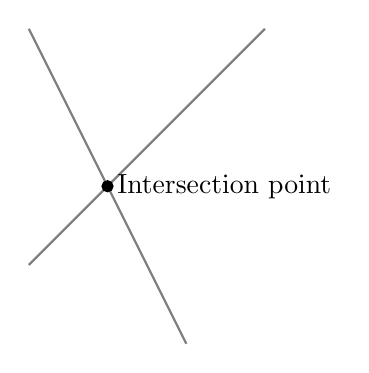
\begin{tikzpicture}
   \draw[gray, thick] (-1,2) -- (1,-2);
   \draw[gray, thick] (-1,-1) -- (2,2);
   \filldraw[black] (0,0) circle (2pt) node[anchor=west] {Intersection point};
  \end{tikzpicture}
  \begin{tikzpicture}
    \draw (-2,0) -- (2,0);
    \filldraw [gray] (0,0) circle (2pt);
    \draw (-2,-2) .. controls (0,0) .. (2,-2);
    \draw (-2,2) .. controls (-1,0) and (1,0) .. (2,2);
  \end{tikzpicture}
  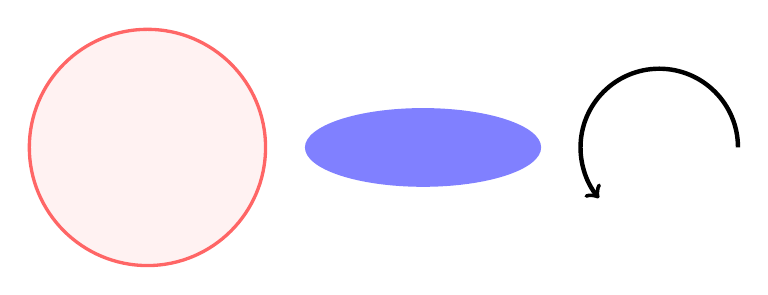
\begin{tikzpicture}
    \filldraw[color=red!60, fill=red!5, very thick](-1,0) circle (1.5);
    \fill[blue!50] (2.5,0) ellipse (1.5 and 0.5);
    \draw[ultra thick, ->] (6.5,0) arc (0:220:1);
  \end{tikzpicture}
\end{tcblisting}

\begin{tcblisting}{title=画图}
  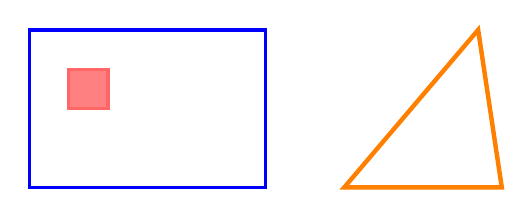
\begin{tikzpicture}
    \filldraw[color=red!60, fill=red!50, very thick](1,1) rectangle (0.5,1.5);
    \draw[blue, very thick] (0,0)rectangle (3,2);
    \draw[orange, ultra thick] (4,0) -- (6,0) -- (5.7,2) -- cycle;
  \end{tikzpicture}
\end{tcblisting}

%% 关联图
\tikz[remember picture] \node[fill=green!30] (n3) {$\sum_{n=1}^{\infty}\frac{1}{n^2}=\frac{\pi^2}{6}$};

\tikz[remember picture]
\node[
	color=red!20,
%	circle,
	draw,
%	label=angle:text,
	fill=red,
	] (nodename) {
	contents
};

%
here is some text\quad\qquad\tikz[remember picture]
\node[
	color=yellow!10,
	%	circle,
	draw,
	%	label=angle:text,
	fill=blue!20,
] (n1) {
	$\sum_{n=1}^{\infty}$
};

\tikz[remember picture]
\draw[overlay,->,very thick,red,opacity=.5]
(nodename) to[bend left] (n1);

here is a circle I will type more words: \tikz[remember picture] \node[fill=red!50] (n1) {$f(x)=\sin x$};

here is a node: \tikz[remember picture] \node[fill=blue!50] (n2) {$f(x)=\sin x$};

\begin{tikzpicture}[remember picture,overlay]
	\draw[->,very thick] (n1) -- (n2);
\end{tikzpicture}

\begin{tikzpicture}[remember picture]
	\node (c) [fill=yellow!20] {Big circle};
	
	\draw[overlay,->,very thick,red,opacity=.5]
	(c) to[bend right] (n1) (n1) -| (n2) (n3) to[bend left] (n1);
\end{tikzpicture}

\begin{tcblisting}{title=270226}
  \definecolor{myred}{RGB}{183,18,52}
  \definecolor{myyellow}{RGB}{254,213,1}
  \definecolor{myblue}{RGB}{0,80,198}
  \definecolor{mygreen}{RGB}{0,155,72}
  \begin{tikzpicture}[
    line join=round,
    y={(-0.86cm,0.36cm)},x={(1cm,0.36cm)}, z={(0cm,1cm)},
    arr/.style={-latex,ultra thick,line cap=round,shorten <= 1.5pt}
  ]
  \def\Side{2}
  \coordinate (A1) at (0,0,0);
  \coordinate (A2) at (0,\Side,0);
  \coordinate (A3) at (\Side,\Side,0);
  \coordinate (A4) at (\Side,0,0);
  \coordinate (B1) at (0,0,\Side);
  \coordinate (B2) at (0,\Side,\Side);
  \coordinate (B3) at (\Side,\Side,\Side);
  \coordinate (B4) at (\Side,0,\Side);

  \fill[myyellow] (A2) -- (A3) -- (B3) -- (B2) -- cycle;
  \fill[mygreen]  (A2) -- (A3) -- (A4) -- (A1) -- cycle;
  \fill[myred](A3) -- (B3) -- (B4) -- (A4) -- cycle;
  \fill[myblue]   (A1) -- (A2) -- (B2) -- (B1) -- cycle;

  \draw (A2) -- (A1) -- (A4);
  \draw (B2) -- (B1) -- (B4) -- (B3) -- cycle;
  \draw (A1) -- (B1);
  \draw (A2) -- (B2);
  \draw (A4) -- (B4);

  \draw[thin] (A3) -- (B3);
  \draw[thin] (A3) -- (A4);

  \path[arr] 
    (A1) edge (A2)
    (B2) edge (A2)
    (B1) edge (B2)
    (B1) edge (A1)
    (B4) edge (A4)
    (B3) edge (A3)
    (B4) edge (B3)
    (A4) edge (A3);

  \node[below] at (A1) {$A$};
  \node[below] at (A2) {$B$};
  \node[below] at (A3) {$C$};
  \node[below] at (A4) {$D$};
  \node[above] at (B1) {$E$};
  \node[above] at (B2) {$F$};
  \node[above] at (B3) {$G$};
  \node[above] at (B4) {$H$};
  \end{tikzpicture}
\end{tcblisting}

\begin{tcblisting}{title=根据三点画弧}
  \begin{tikzpicture}
    \tkzDefPoint(1,2){A}
    \tkzDefPoint(3,4){B}
    \tkzDefPoint(2,4){C}
    \tkzCircumCenter(A,B,C)\tkzGetPoint{O}
    \tkzDrawArc(O,C)(A)
  \end{tikzpicture}
\end{tcblisting}


\begin{tcblisting}{title=字体}
  $\mathscr{ABCDEFGHIJKLMNOPQRSTUVWXYZ}$\\
  $\mathbb{ABCDEFGHIJKLMNOPQRSTUVWXYZ}$\\
  $\mathcal{ABCDEFGHIJKLMNOPQRSTUVWXYZ}$\\
  $\mathfrak{ABCDEFGHIJKLMNOPQRSTUVWXYZ}$
\end{tcblisting}

\section{pstricks}
{\black this is black.}
{\darkgray this is darkgray.}
{\gray this is gray.}
{\lightgray this is lightgray.}
{\white this is white.}

{\red this is red.}
{\green this is green.}
{\blue this is blue.}
{\cyan this is cyan.}
{\magenta this is magenta.}
{\yellow this is yellow.}

%{\psset{linecolor=green,linestyle=dotted}\psline(8,7)}

%\begin{tcblisting}
%	
%\end{tcblisting}

\section{asymptote}

\begin{tcblisting}{title=Asymptote}
	\begin{asy}
		include graph;
		size(1inch);
		filldraw(circle((0,0),1),yellow,black);
		fill(circle((-.3,.4),.1),black);
		fill(circle((.3,.4),.1),black);
		draw(arc((0,0),.5,-140,-40));
	\end{asy}
\end{tcblisting}

\begin{tcblisting}{title=Transform}
	\begin{center}
		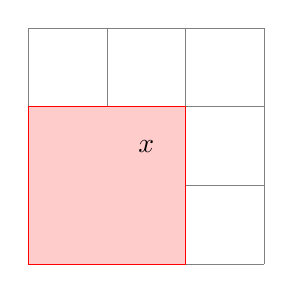
\begin{tikzpicture}[remember picture]
			\draw[help lines] (0,0) grid (3,3);
			\draw[red,fill=red!20] (0,0)--(2,0)--(2,2)--(0,2)--(0,0); 
			\node (n3) at (1.5,1.5) {$x$};
		\end{tikzpicture}
		\hspace{3mm}
		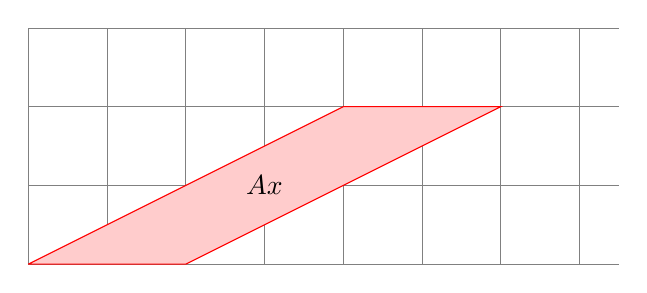
\begin{tikzpicture}[remember picture]
			\draw[help lines] (0,0) grid (7.5,3);
			\draw[red,fill=red!20] (0,0)--(2,0)--(6,2)--(4,2)--(0,0); 
			\node (n2) at (3,1) {$Ax$};
		\end{tikzpicture}
		\begin{tikzpicture}[remember picture,overlay]
			\draw[overlay,->,very thick] (n3) to[bend left] (n2);
		\end{tikzpicture}
	\end{center}
\end{tcblisting}

\newpage


% \chapter{math.stackexchange.com}
%%%%%%%%%%%%%%%%%%%%%%%%%%%%%%%%%%%%%%%%%%%%%%%
%%%%%%%%%%%%%%%%%%%%%%%%%%%%%%%%%%%%%%%%%%%%%%%
\bqq[breakable]{1. What Does it Really Mean to Have Different Kinds of Infinities?}{1}
What Does it Really Mean to Have Different Kinds of Infinities?

Can someone explain to me how there can be different kinds of infinities?

I was reading \href{http://en.wikipedia.org/wiki/The_Man_Who_Loved_Only_Numbers}{The man who loved only numbers}
by \href{http://en.wikipedia.org/wiki/Paul_Hoffman_(science_writer)}{Paul Hoffman}
and came across the concept of countable and uncountable infinities,
but they're only words to me.

Any help would be appreciated. 
\bs
Suppose no one ever taught you the names for ordinary numbers. Then
suppose that you and I agreed that we would trade one bushel of corn
for each of my sheep. But there's a problem, we don't know how to
count the bushels or the sheep! So what do we do?

We form a  bijection between the two
sets. That's just fancy language for saying you pair things up by
putting one bushel next to each of the sheep. When we're done we swap.
We've just proved that the number of sheep is the same as the number
of bushels without actually counting.

We can try doing the same thing with infinite sets. So suppose you
have the set of positive integers and I have the set of rational numbers
and you want to trade me one positive integer for each of my rationals.
Can you do so in a way that gets all of my rational numbers?

Perhaps surprisingly the answer is yes! You make the rational numbers
into a big square grid with the numerator and denominators as the
two coordinates. Then you start placing your  bushels
along diagonals of increasing size, \href{http://en.wikipedia.org/wiki/File:Pairing_natural.svg}{see wikipedia}.

This says that the rational numbers are  countable
that is you can find a clever way to count them off in the above fashion.

The remarkable fact is that for the real numbers there's no way at
all to count them off in this way. No matter how clever you are you
won't be able to scam me out of all of my real numbers by placing
a natural number next to each of them. The proof of that is Cantor's
clever \href{http://en.wikipedia.org/wiki/Cantor's_diagonal_argument}{diagonal argument}.
\bm
Fantastic answer! -- Allain Lalonde

I like this so far, but maybe add a bit on uncountable to distinguish
the difference. -- BBischof

That's a really good answer, thanks :D -- fbstj

Why can't lecturers at Uni explain things in this way? -- Sachin
Kainth

In the case of positives and rationals how you match them? How diagonals
become  bushels . Can u explain more on
that figure -- user5507

+1 for  fancy language -- Tyler Langan

Wow, great way to explain it. -- Abhimanyu Pallavi Sudhir

One bushel of corn for each sheep is a little too generous for me.
:P -- BlackAdder

OMG I love the bushels and the sheep. Very great way to explain it.
-- Brian Cheung

I assume with  positive numbers you mean
 positive integers . Because, after all,
$\pi$ is a positive number as well. -- celtschk
\em
\es
\bs
\textbf{How there can be different kinds of infinities?}

This is very simple to see. This is because of:

Claim: A given set $X$ and its power set $P(X)$ can never be in
bijection. 

Proof: By contradiction. Let $f$ be any function from $X$ to $P(X)$.
It suffices to prove $f$ cannot be surjective. That means that some
member of $P(X)$ i.e., some subset of $S$, is not in the image of
$f$. Consider the set:

$T=\{ x\in X: x\not\in f(x) \}.$

For every $x$ in $X$ , either $x$ is in $T$ or not. If $x$ is
in $T$, then by definition of $T$, $x$ is not in $f(x)$, so $T$
is not equal to $f(x)$. On the other hand, if $s$ is not in $T$,
then by definition of $T$, $x$ is in $f(x)$, so again $T$ is not
equal to $f(x)$. Q.E.D.

Thus take any infinite set you like. Then take its power set, its
power set, and so on. You get an infinite sequence of sets of increasing
cardinality(Here I am skipping a little; but a use of the Schroeder-Bernstein
theorem will fix things).

\href{http://en.wikipedia.org/wiki/Hilbert\%27s_paradox_of_the_Grand_Hotel}{Hilbert's Hotel}
is a classic demonstration.
\es
\bs
\href{http://en.wikipedia.org/wiki/Hilbert\%27s_paradox_of_the_Grand_Hotel}{Hilbert's Hotel} is a classic demonstration.
\bm
A really good book on the subject was written by David Wallace Foster, 
\href{http://www.amazon.co.uk/Everything-More-Compact-History-Infinity/dp/0753818825/ref=ntt_at_ep_dpt_10}{Everything and More: A Compact History of Infinity} – FordBuchanan

David Foster Wallace. (RIP :-( ) – Jason S
\em
\es
\bs
A \textbf{countably infinite} set is a set for which you can list
the elements $a_1,a_2,a_3,...$

For example, the set of all integers is countably infinite since I
can list its elements as follows: 

$0,1,-1,2,-2,3,-3,...$ 

So is the set of rational numbers, but this is more difficult to see.
Let's start with the positive rationals. Can you see the pattern in
this listing?

$\frac{1}{1},\frac{1}{2},\frac{2}{1},\frac{1}{3},\frac{2}{2},\frac{3}{1},\frac{1}{4},\frac{2}{3},\frac{3}{2},\frac{4}{1},\frac{1}{5},\frac{2}{4},...$

(Hint: Add the numerator and denominator to see a different pattern.) 

This listing has lots of repeats, e.g. $\frac{1}{1}, \frac{2}{2}$
and $\frac{1}{2}, \frac{2}{4}$. That's ok since I can condense the
listing by skipping over any repeats.

$\frac{1}{1},\frac{1}{2},\frac{2}{1},\frac{1}{3},\frac{3}{1},\frac{1}{4},\frac{2}{3},\frac{3}{2},\frac{4}{1},\frac{1}{5},...$

Let's write $q_n$ for the $n$-th element of this list. Then $0,q_1,-q_1,q_2,-q_2,q_3,-q_3,...$
is a listing of all rational numbers.

A \textbf{countable set} is a set which is either finite or countably
infinite; an \textbf{uncountable set} is a set which is not countable.

Thus, an uncountable set is an infinite set which has no listing of
all of its elements (as in the definition of countably infinite set).

An example of an uncountable set is the set of all real numbers. To
see this, you can use the \textbf{diagonal method}. Ask another question
to see how this works...
\es
\eqq

% \chapter{语录}
\begin{verbatim}
在我年轻的时候, 我听从建议去读庞加莱, 希尔伯特, 克莱因以及胡尔维茨等的著作,
并从中获益. 而我自己对布拉须凯, 嘉当和霍普夫的著作更为熟悉, 其实这也是中国
的传统: 在中国我们被教导要读孔夫子, 韩愈的散文以及杜甫的诗歌, 我真诚地希望
这套全集不要成为书架上的摆设, 而是在年轻数学家的手里被翻烂掉.
\end{verbatim}

% verbatim
\begin{verbatim}
有人主张依靠直观去进行数学教学, 我却认为再没有比这种数学教学方法更为荒谬和
更为有害的了, 每一个数学教师都应当不遗余力地教会学生去思考而不依赖于直观感觉.
--柯勒里吉
\end{verbatim}

% verbatim
\begin{verbatim}
数学不是规律的发现者, 因为它不是归纳. 数学也不是理论的缔造者, 因为他不是假说.
但数学却是规律和理论的裁判和主宰者. 因为规律和假说都要向数学表明自己的主张,
然后等待数学的裁判. 如果没有数学上的认可, 则规律不能起作用, 理论也不能解释.
--Peirce, Benjamin
\end{verbatim}



\newpage

\end{CJK}
\end{document}
